% !TeX program = xelatex
% !TeX TXS-program:compile = txs:///xelatex/[--shell-escape]
%%%%%%%%%%%%%%%%%%%%%%%%%%%%%%%%%%%%%%%%%%%%%%%%%%%%%%%%%%%%%%%%%%%%%%%%
% Plantilla TFG/TFM
% Escuela Politécnica Superior de la Universidad de Alicante
% Realizado por: Jose Manuel Requena Plens
% Contacto: info@jmrplens.com / Telegram:@jmrplens
%%%%%%%%%%%%%%%%%%%%%%%%%%%%%%%%%%%%%%%%%%%%%%%%%%%%%%%%%%%%%%%%%%%%%%%%

% Elige si deseas optimizar la ejecución del proyecto almacenando las figuras generadas con TikZ y PGF en una carpeta (archivos/figuras-procesadas).
% 1 - Si, 2 - No
\def\OptimizaTikZ{1}

% Archivo .TEX que incluye todas las configuraciones del documento y los paquetes. Añade todo aquello que necesites utilizar en el documento en este archivo.
% En él se encuentra la configuración de los márgenes, establecidos según las directrices de estilo de la EPS.
%%%%%%%%%%%%%%%%%%%%%%%%%%%%%%%%%%%%%%%%%%%%%%%%%%%%%%%%%%%%%%%%%%%%%%%%
% Plantilla TFG/TFM
% Escuela Politécnica Superior de la Universidad de Alicante
% Realizado por: Jose Manuel Requena Plens
% Contacto: info@jmrplens.com / Telegram:@jmrplens
%%%%%%%%%%%%%%%%%%%%%%%%%%%%%%%%%%%%%%%%%%%%%%%%%%%%%%%%%%%%%%%%%%%%%%%%

%%%%%%%%%%%%%%%%%%%%%%%%
% FORMATO DEL DOCUMENTO
%%%%%%%%%%%%%%%%%%%%%%%%
% scrbook es la clase de documento
% Si se desea que no haya página en blanco entre capítulos añadir "openany" en los parámetros de la clase. Sino siempre los capítulos empezarán en página impar.
\documentclass[a4paper,11pt,titlepage]{scrbook}
\KOMAoption{toc}{bib,chapterentryfill} % Opciones del índice
\usepackage{scrhack} % Previene algunos errores
% Paquete de formato para scrbook. Con marcas, linea-separador superior e inferior
\usepackage[automark,headsepline,footsepline]{scrlayer-scrpage}
\clearpairofpagestyles		% Borra los estilos por defecto
%%
% Formato y contenido de la información de cabecera y pie de página
%%
% Información de capítulo en cabecera e interno
\ihead{{\color{gray30}\scshape\small\headmark}}	
% Número de página en cabecera y externo
\ohead{\normalfont\pagemark} 
% Número de página en pie de página y externo. Sólo en páginas sin cabecera
\ofoot[\normalfont\pagemark]{}
%% 		
% Edición del contenido de las distintas partes de la cabecera
%%
\renewcommand{\chaptermark}[1]{\markboth{#1}{}} % Capítulo (Solo texto)
\renewcommand{\sectionmark}[1]{\markright{\thesection. #1}} % Sección (Número y texto)
\setkomafont{pagenumber}{} % Número de página (Sin nada añadido)

% Añade al índice y numera hasta la profundidad 4.
% 1:section,2:subsection,3:subsubsection,4:paragraph
\setcounter{tocdepth}{4}
\setcounter{secnumdepth}{4}
% Muestra una regla para comprobar el formato de las páginas
%\usepackage[type=upperleft,showframe,marklength=8mm]{fgruler}
% MÁRGENES DE LAS PÁGINAS
\usepackage[
  inner	=	3.0cm, % Margen interior
  outer	=	2.5cm, % Margen exterior
  top	=	2.5cm, % Margen superior
  bottom=	2.5cm, % Margen inferior
  includeheadfoot, % Incluye cabecera y pie de página en los márgenes
]{geometry}
% Valor de interlineado
\renewcommand{\baselinestretch}{1.0} % 1 línea de interlineado
% Para poder generar páginas horizontales
\usepackage{lscape}
% Ancho de la zona para comentarios en el margen. (modificado para todonotes)
\setlength{\marginparwidth}{1.9cm}

%%%%%%%%%%%%%%%%%%%%%%%%
% BIBLIOGRAFÍA
%%%%%%%%%%%%%%%%%%%%%%%%
\usepackage{apacite} % NORMA APA
\usepackage{natbib}
\usepackage{breakcites}

%%%%%%%%%%%%%%%%%%%%%%%%
% DOCUMENTO EN ESPAÑOL
%%%%%%%%%%%%%%%%%%%%%%%%
\usepackage[base]{babel}
\usepackage{polyglossia}
\setdefaultlanguage{spanish}

\addto\captionsspanish{%
	\renewcommand{\listtablename}{Índice de tablas} 
	\renewcommand{\tablename}{Tabla}
	\renewcommand{\lstlistingname}{Código}
	\renewcommand{\lstlistlistingname}{Índice de \lstlistingname s}
	\renewcommand{\glossaryname}{Glosario}
	\renewcommand{\acronymname}{Acrónimos}
	\renewcommand{\bibname}{Bibliografía}%
}

%%%%%%%%%%%%%%%%%%%%%%%% 
% COLORES
%%%%%%%%%%%%%%%%%%%%%%%% 
% Biblioteca de colores
\usepackage{color}
\usepackage[dvipsnames]{xcolor}
% Otros colores definidos por el usuario
\definecolor{gray97}{gray}{.97}
\definecolor{gray75}{gray}{.75}
\definecolor{gray45}{gray}{.45}
\definecolor{gray30}{gray}{.30}
\definecolor{negro}{RGB}{0,0,0}
\definecolor{blanco}{RGB}{255,255,255}
\definecolor{dkgreen}{rgb}{0,.6,0}
\definecolor{dkblue}{rgb}{0,0,.6}
\definecolor{dkyellow}{cmyk}{0,0,.8,.3}
\definecolor{gray}{rgb}{0.5,0.5,0.5}
\definecolor{mauve}{rgb}{0.58,0,0.82}
\definecolor{deepblue}{rgb}{0,0,0.5}
\definecolor{deepred}{rgb}{0.6,0,0}
\definecolor{deepgreen}{rgb}{0,0.5,0}
\definecolor{MyDarkGreen}{rgb}{0.0,0.4,0.0}
\definecolor{bluekeywords}{rgb}{0.13,0.13,1}
\definecolor{greencomments}{rgb}{0,0.5,0}
\definecolor{redstrings}{rgb}{0.9,0,0}

%%%%%%%%%%%%%%%%%%%%%%%%
% TABLAS
%%%%%%%%%%%%%%%%%%%%%%%%
% Paquetes para tablas
\usepackage{longtable,booktabs,array,multirow,multicol,tabularx,ragged2e,array}
% Nuevos tipos de columna para tabla, se pueden utilizar como por ejemplo C{3cm} en la definición de columnas de la función tabular
\newcolumntype{L}[1]{>{\raggedright\let\newline\\\arraybackslash\hspace{0pt}}m{#1}}
\newcolumntype{C}[1]{>{\centering\let\newline\\\arraybackslash\hspace{0pt}}m{#1}}
\newcolumntype{R}[1]{>{\raggedleft\let\newline\\\arraybackslash\hspace{0pt}}m{#1}}

%%%%%%%%%%%%%%%%%%%%%%%% 
% GRAFICAS y DIAGRAMAS 
%%%%%%%%%%%%%%%%%%%%%%%% 
% Paquete para todo tipo de gráficas, diagramas, modificación de imágenes, etc
\usepackage{tikz,tikzpagenodes}
\usetikzlibrary{tikzmark,calc,shapes.geometric,arrows,backgrounds,shadings,shapes.arrows,shapes.symbols,shadows,positioning,fit,automata,patterns,intersections}
\usepackage{pgfplots}
\pgfplotsset{colormap/jet}
\pgfplotsset{compat=newest} % Compatibilidad
\usepgfplotslibrary{patchplots,groupplots,fillbetween,polar}
\usepackage{pgfplotstable}
% Guardar las figuras realizadas con Tikz y Pgf en una carpeta externa
% para agilizar el procesado y tenerlas para utilizarlas en otros
% documentos
\if\OptimizaTikZ 1
\usepgfplotslibrary{external}
\tikzexternalize[prefix=archivos/figuras-procesadas/] % Ruta
\tikzset{%
    external/system call ={xelatex -enable-write18 -halt-on-error -interaction=batchmode -jobname "\image" "\texsource"},
}
\fi

% Estilos para elementos graficos
% Cajas y cajas de texto
\tikzstyle{Caja1} = [green,very thick,rounded corners,fill=white, fill opacity=0.5]
\tikzstyle{Texto1} = [fill=white,thick,shape=circle,draw=black,inner sep=2pt,font=\sffamily,text=black]
\tikzstyle{Texto2} = [fill=white,thick,shape=rectangle,draw=black,inner sep=2pt,font=\sffamily,text=black]
\tikzstyle{Texto3} = [fill=white,thick,shape=circle,draw=black,inner sep=2pt,font=\sffamily,text=black]
% Cuadros de diagrama
\tikzstyle{rectvioleta} = [rectangle, rounded corners, text centered, draw=black, fill=blue!10]
\tikzstyle{rectnaranja} = [rectangle, minimum width=2cm, minimum height=1cm, text centered, draw=black, fill=orange!10]
\tikzstyle{romborosa} = [diamond, aspect=3, minimum width=3cm, minimum height=1cm, text centered, draw=black, fill=red!10]
\tikzstyle{rectverde} = [rectangle, minimum width=2cm, minimum height=1cm, text centered, draw=black, fill=green!10]
\tikzstyle{rectamarillo} = [rectangle, rounded corners, minimum width=2cm, minimum height=1cm, text centered, draw=black, fill=yellow!10]
% Flechas
\tikzstyle{arrow} = [thick,->,>=stealth]

%%%%%%%%%%%%%%%%%%%%%%%% 
% FIGURAS, TABLAS, ETC 
%%%%%%%%%%%%%%%%%%%%%%%% 
\usepackage{subcaption} % Para poder realizar subfiguras
\usepackage{caption} % Para aumentar las opciones de diseño
% Nombres de figuras, tablas, etc, en negrita la numeración, todo con letra small
\captionsetup{labelfont={bf,small},textfont=small}
% Paquete para modificar los espacios arriba y abajo de una figura o tabla
\usepackage{setspace}
% Define el espacio tanto arriba como abajo de las figuras, tablas
\setlength{\intextsep}{5mm}
% Para ajustar tamaños de texto de toda una tabla o grafica
% Uso: {\scalefont{0.8} \begin{...} \end{...} }
\usepackage{scalefnt}
% Redefine las tablas y figuras para eliminar el '.' entre la numeración y el texto
\renewcommand*{\figureformat}{\figurename~\thefigure}
\renewcommand*{\tableformat}{\tablename~\thetable}

%%%%%%%%%%%%%%%%%%%%%%%% 
% TEXTO
%%%%%%%%%%%%%%%%%%%%%%%%
% Paquete para poder modificar las fuente de texto
\usepackage{xltxtra}
% Cualquier tamaño de texto. Uso: {\fontsize{100pt}{120pt}\selectfont tutexto}
\usepackage{anyfontsize}
% Para modificar parametros del texto.
\usepackage{setspace}
% Paquete para posicionar bloques de texto
\usepackage{textpos}
% Paquete para realizar cajas de texto. 
% Uso: \begin{mdframed}[linecolor=red!100!black] tutexto \end{mdframed}
\usepackage{framed,mdframed}
% Para subrayar. Uso: \hlc[tucolor]{tutexto}
\newcommand{\hlc}[2][yellow]{ {\sethlcolor{#1} \hl{#2}} }

%%%%%%%%%%%%%%%%%%%%%%%% 
% OTROS
%%%%%%%%%%%%%%%%%%%%%%%%
% Para hacer una pagina horizontal. Uso: \begin{landscape} xxxx \end{lanscape}
\usepackage{lscape} 
% Para incluir paginas PDF. Uso:
% \includepdf[pages={1}]{tuarchivo.pdf}
\usepackage{pdfpages}
% Para introducir url's con formato. Uso: \url{http://www.google.es}
\usepackage{url}
% Amplia muchas funciones graficas de latex
\usepackage{graphicx}
% Paquete que añade el hipervinculo en referencias dentro del documento, indice, etc
% Se define sin bordes alrededor. Uso: \ref{tulabel}
\usepackage[pdfborder={000}]{hyperref}
\usepackage{float}
\usepackage{placeins}
\usepackage{afterpage}
\usepackage{verbatim}
% Paquete para condicionales avanzados
\usepackage{xstring,xifthen}
% Paquete para realizar calculos en el código
\usepackage{calc}
% Para rotar tablas o figuras o su contenido
\usepackage{rotating} 
% Para incluir comentarios en el texto. El parámetro 'disable' oculta todas las notas.
% USO: \todo{tutexto}
\usepackage[textsize=tiny,spanish,shadow,textwidth=2cm]{todonotes}
%\reversemarginpar % Descomentar si se quiere todos los comentarios en el mismo lado
% Desactiva la exportación de los ToDo y Missingfigures como figuras
\if\OptimizaTikZ 1
\makeatletter
\renewcommand{\todo}[2][]{\tikzexternaldisable\@todo[#1]{#2}\tikzexternalenable}
\makeatother
\usepackage{letltxmacro}
\LetLtxMacro{\oldmissingfigure}{\missingfigure}
\makeatletter
\renewcommand{\missingfigure}[2][]{\tikzexternaldisable\oldmissingfigure[{#1}]{#2}\tikzexternalenable}
\makeatother
\fi

%%%%%%%%%%%%%%%%%%%%%%%% 
% GLOSARIOS
%%%%%%%%%%%%%%%%%%%%%%%%
\usepackage[acronym,nonumberlist,toc]{glossaries}
\usepackage{glossary-superragged}
\newglossarystyle{modsuper}{%
  \setglossarystyle{super}%
  \renewcommand{\glsgroupskip}{}
}
\renewcommand{\glsnamefont}[1]{\textbf{#1}}


%%%%%%%%%%%%%%%%%%%%%%%% 
% COMANDOS AÑADIDOS
%%%%%%%%%%%%%%%%%%%%%%%%
% Para mostrar la fecha actual (mes año) con \Hoy
\newcommand{\MES}{%
  \ifcase\month% 0
    \or Enero% 1
    \or Febrero% 2
    \or Marzo% 3
    \or Abril% 4
    \or Mayo% 5
    \or Junio% 6
    \or Julio% 7
    \or Agosto% 8
    \or Septiembre% 9
    \or Octubre% 10
    \or Noviembre% 11
    \or Diciembre% 12
  \fi}
\newcommand{\ANYO}{\number\year}
\newcommand{\Hoy}{\MES\ \ANYO}

%%%%%%%%%%%%%%%%%%%%%%%% 
% MATEMÁTICAS
%%%%%%%%%%%%%%%%%%%%%%%%
\usepackage{mathtools,amsthm,amsfonts,amssymb,bm,mathrsfs,nicefrac,upgreek,bigints} 
% Comando para añadir información de variables a las ecuaciones
% Uso: \begin{condiciones}[donde:] ....... \end{condiciones}
\newenvironment{condiciones}[1][2]
  {%
   #1\tabularx{\textwidth-\widthof{#1}}[t]{
     >{$}l<{$} @{}>{${}}c<{{}$}@{} >{\raggedright\arraybackslash}X
   }%
  }
  {\endtabularx\\[\belowdisplayskip]}

%%%%%
% PARÁMETROS DE FORMATO DE CODIGOS
%%%%%
% Puedes editar los formatos para ajustarlos a tu gusto
%%%%%%%%%%%%%%%%%%%%%%%%%%%%%%%%%%%%%%%%%%%%%%%%%%%%%%%%%%%%%%%%%%%%%%%%
% Plantilla TFG/TFM
% Escuela Politécnica Superior de la Universidad de Alicante
% Realizado por: Jose Manuel Requena Plens
% Contacto: info@jmrplens.com / Telegram:@jmrplens
%%%%%%%%%%%%%%%%%%%%%%%%%%%%%%%%%%%%%%%%%%%%%%%%%%%%%%%%%%%%%%%%%%%%%%%%


%%%%%%%%%%%%%%%%%%%%%%%% 
% CÓDIGO. CONFIGURACIÓN. En el siguiente bloque están los estilos.
%%%%%%%%%%%%%%%%%%%%%%%%
% Paquete para mostrar código de matlab. En caja y lineas numeradas
\usepackage[framed,numbered]{matlab-prettifier}
% Paquete mostrar código de programación de distintos lenguajes
\usepackage{listings}
\lstset{ inputencoding=utf8,
extendedchars=true,
frame=single, % Caja donde se ubica el código
backgroundcolor=\color{gray97}, % Color del fondo de la caja
rulesepcolor=\color{black},
boxpos=c,
abovecaptionskip=-4pt,
aboveskip=12pt,
belowskip=0pt,
lineskip=0pt,
framerule=0pt,
framextopmargin=4pt,
framexbottommargin=4pt,
framexleftmargin=11pt,
framexrightmargin=0pt,
linewidth=\linewidth,
xleftmargin=\parindent,
framesep=0pt,
rulesep=.4pt,
stringstyle=\ttfamily,
showstringspaces = false,
showspaces = false,
showtabs = false,
columns=fullflexible,
basicstyle=\small\ttfamily,
commentstyle=\color{gray45},
keywordstyle=\bfseries,
tabsize=4,
numbers=left,
numbersep=1pt,
numberstyle=\tiny\ttfamily\color{gray75},
numberfirstline = false,
breaklines=true,
postbreak=\mbox{\textcolor{red}{$\hookrightarrow$}\space}, % Flecha al saltar de linea
prebreak=\mbox{\textcolor{red}{$\hookleftarrow$}\space}, % Flecha al saltar de linea
literate=
  {á}{{\'a}}1 {é}{{\'e}}1 {í}{{\'i}}1 {ó}{{\'o}}1 {ú}{{\'u}}1
  {Á}{{\'A}}1 {É}{{\'E}}1 {Í}{{\'I}}1 {Ó}{{\'O}}1 {Ú}{{\'U}}1
  {à}{{\`a}}1 {è}{{\`e}}1 {ì}{{\`i}}1 {ò}{{\`o}}1 {ù}{{\`u}}1
  {À}{{\`A}}1 {È}{{\'E}}1 {Ì}{{\`I}}1 {Ò}{{\`O}}1 {Ù}{{\`U}}1
  {ä}{{\"a}}1 {ë}{{\"e}}1 {ï}{{\"i}}1 {ö}{{\"o}}1 {ü}{{\"u}}1
  {Ä}{{\"A}}1 {Ë}{{\"E}}1 {Ï}{{\"I}}1 {Ö}{{\"O}}1 {Ü}{{\"U}}1
  {â}{{\^a}}1 {ê}{{\^e}}1 {î}{{\^i}}1 {ô}{{\^o}}1 {û}{{\^u}}1
  {Â}{{\^A}}1 {Ê}{{\^E}}1 {Î}{{\^I}}1 {Ô}{{\^O}}1 {Û}{{\^U}}1
  {œ}{{\oe}}1 {Œ}{{\OE}}1 {æ}{{\ae}}1 {Æ}{{\AE}}1 {ß}{{\ss}}1
  {ű}{{\H{u}}}1 {Ű}{{\H{U}}}1 {ő}{{\H{o}}}1 {Ő}{{\H{O}}}1
  {ç}{{\c c}}1 {Ç}{{\c C}}1 {ø}{{\o}}1 {å}{{\r a}}1 {Å}{{\r A}}1
  {€}{{\euro}}1 {£}{{\pounds}}1 {«}{{\guillemotleft}}1
  {»}{{\guillemotright}}1 {ñ}{{\~n}}1 {Ñ}{{\~N}}1 {¿}{{?`}}1,
  }

% Intenta no dividir los códigos en diferentes paginas si es posible
\lstnewenvironment{listing}[1][]
   {\lstset{#1}\pagebreak[0]}{\pagebreak[0]}

% Formato de títulos de los códigos
\DeclareCaptionFont{white}{\color{white}}
\DeclareCaptionFormat{listing}{\colorbox{gray}{\parbox{\textwidth - 2\fboxsep}{#1#2#3}}}
\captionsetup[lstlisting]{format=listing,labelfont=white,textfont=white,font= scriptsize}


%%%%%%%%%%%%%%%%%%%%%%%% 
% CÓDIGO. ESTILOS. Ajústalos a tu gusto
%%%%%%%%%%%%%%%%%%%%%%%%
\lstdefinestyle{Consola}
	{
	basicstyle=\scriptsize\bf\ttfamily,
	}
   
\lstdefinestyle{C}
	{
	basicstyle=\scriptsize,
	language=C,
	}
\lstdefinestyle{C-color}
	{
  	breaklines=true,
  	language=C,
  	basicstyle=\scriptsize,
  	keywordstyle=\bfseries\color{green!40!black},
  	commentstyle=\itshape\color{purple!40!black},
  	identifierstyle=\color{blue},
  	stringstyle=\color{orange},
    }
\lstdefinestyle{CSharp}
	{
	basicstyle=\scriptsize
	language=[Sharp]C,
	escapeinside={(*@}{@*)},
	keywordstyle=\bfseries,
	}
\lstdefinestyle{CSharp-color}
	{
	basicstyle=\scriptsize
	language=[Sharp]C,
	escapeinside={(*@}{@*)},
	commentstyle=\color{greencomments},
	keywordstyle=\color{bluekeywords}\bfseries,
	stringstyle=\color{redstrings},
	}
\lstdefinestyle{C++}
	{
	basicstyle=\scriptsize,
	language=C++,
 	}
 	
\lstdefinestyle{C++-color}
	{
  	breaklines=true,
  	language=C++,
  	basicstyle=\scriptsize,
  	keywordstyle=\bfseries\color{green!40!black},
  	commentstyle=\itshape\color{purple!40!black},
  	identifierstyle=\color{blue},
  	stringstyle=\color{orange},
    }
    
\lstdefinestyle{PHP}
	{
	basicstyle=\scriptsize,
	language=PHP,
	}
	
\lstdefinestyle{PHP-color}
	{
	basicstyle=\scriptsize,
	language=PHP,
	keywordstyle    = \color{dkblue},
  	stringstyle     = \color{red},
  	identifierstyle = \color{dkgreen},
  	commentstyle    = \color{gray},
  	emph            =[1]{php},
  	emphstyle       =[1]\color{black},
  	emph            =[2]{if,and,or,else},
  	emphstyle       =[2]\color{dkyellow}
  }
  
\lstdefinestyle{Matlab}
	{
	basicstyle=\scriptsize,
	language=Matlab,
	numberstyle=\tiny\ttfamily\color{gray75},
	}
	
\lstdefinestyle{Matlab-color}
	{
	style = Matlab-editor,
	basicstyle=\scriptsize,
	numberstyle=\tiny\ttfamily\color{gray75},
	}
	
\lstdefinestyle{Latex}
	{
	language=[LaTeX]{Tex},
    basicstyle=\scriptsize,
    literate={\$}{{{\bfseries\$}}}1,
    alsoletter={\\,*,\&},
    emph =[1]{\\begin,\\end,\\caption,\\label,\\centering,\\FloatBarrier,
              \\lstinputlisting,\\scalefont,\\addplot,\\input,
              \\legend,\\item,\\subitem,\\includegraphics,\\textwidth,
              \\section,\\subsection,\\subsubsection,\\paragraph,
              \\cite,\\citet,\\citep,\\gls,\\bibliographystyle,\\url,
              \\citet*,\\citep*,\\todo,\\missingfigure,\\footnote},
  	emphstyle =[1]\bfseries,
  	emph = [2]{equation,subequations,eqnarray,figure,subfigure,
  			   condiciones,flalign,tikzpicture,axis,lstlisting,
  			   itemize,description
  			   },
  	emphstyle =[2]\bfseries,
    numbers=none,
	}
	
\lstdefinestyle{Latex-color}
	{
	language=[LaTeX]{Tex},
    basicstyle=\scriptsize,
    commentstyle=\color{dkgreen},
    identifierstyle=\color{black},
    literate={\$}{{{\bfseries\color{Dandelion}\$}}}1, % Colorea el simbolo dollar
    alsoletter={\\,*,\&},
    emph =[1]{\\begin,\\end,\\caption,\\label,\\centering,\\FloatBarrier,
              \\lstinputlisting,\\scalefont,\\addplot,\\input,
              \\legend,\\item,\\subitem,\\includegraphics,\\textwidth,
              \\section,\\subsection,\\subsubsection,\\paragraph,
              \\cite,\\citet,\\citep,\\gls,\\bibliographystyle,\\url,
              \\citet*,\\citep*,\\todo,\\missingfigure,\\footnote},
  	emphstyle =[1]\bfseries\color{RoyalBlue},
  	emph = [2]{equation,subequations,eqnarray,figure,subfigure,
  			   condiciones,flalign,tikzpicture,axis,lstlisting,
  			   itemize,description
  			   },
  	emphstyle =[2]\bfseries,
    numbers=none,
	}
\lstdefinestyle{Java}
{
	basicstyle=\scriptsize,
	language=Java,
}

\lstdefinestyle{Java-color}
{
	basicstyle=\scriptsize,
	language=Java,
  	keywordstyle=\color{blue},
  	commentstyle=\color{dkgreen},
  	stringstyle=\color{mauve},
}
\lstdefinestyle{Python}
{
	language=Python,
	basicstyle=\scriptsize,
	otherkeywords={self},  
	keywordstyle=\bfseries,     
	emphstyle=\bfseries,    
	emph={MyClass,__init__},         
}

\lstdefinestyle{Python-color}
{
	language=Python,
	basicstyle=\scriptsize,
	otherkeywords={self},          
	keywordstyle=\bfseries\color{deepblue},
	emph={MyClass,__init__},         
	emphstyle=\bfseries\color{deepred},    
	stringstyle=\color{deepgreen},
}
\lstdefinestyle{R}
{
	language=R,                     
  	basicstyle=\scriptsize,
  	keywordstyle=\bfseries, 
}
\lstdefinestyle{R-color}
{
	language=R,                     
  	basicstyle=\scriptsize,
  	keywordstyle=\bfseries\color{RoyalBlue}, 
  	commentstyle=\color{YellowGreen},
  	stringstyle=\color{ForestGreen}  
}


%%%%%
% DEFINICION DE CONCEPTOS
%%%%
% Uso ejemplo: \begin{ejemplo} tucontenido \end{ejemplo} 
\newtheorem{teorema}{Teorema}[chapter]
\newtheorem{ejemplo}{Ejemplo}[chapter]
\newtheorem{definicion}{Definición}[chapter]



%%%%%%%%%%%%%%%%%%%%%%%%%%%%%%%%%%%%%%%%%%%%%%%%%%%%%%%%%%%%%%%%%%%%%%
% INFORMACIÓN DEL TFG
% Comentar lo que NO se desee añadir y sustituir con la información correcta.
%%%%%%%%%%%%%%%%%%%%%%%%%%%%%%%%%%%%%%%%%%%%%%%%%%%%%%%%%%%%%%%%%%%%%%
% Título y subtítulo
\newcommand{\titulo}{Demo técnica para PC}
\newcommand{\subtitulo}{La demoscene}
% Datos del autor
\newcommand{\miNombre}{Luis González Aracil}
\newcommand{\miEmail}{lga42@alu.ua.es}
% Datos del tutor/es
\newcommand{\miTutor}{Francisco José Gallego Durán}
\newcommand{\departamentoTutor}{Ciencia de la Computación e Inteligencia Artificial}
% Datos de la facultada y universidad
\newcommand{\miFacultad}{Escuela Politécnica Superior}
\newcommand{\miFacultadCorto}{EPS UA}
\newcommand{\miUniversidad}{\protect{Universidad de Alicante}}
\newcommand{\miUbicacion}{Alicante}

%%%%%%%%%%%%%%%%%%%%%%%%%%%%%%%%%%%%%%%%%%%%%%%%%%%%%%%%%%%%%%%%%%%%%%
% INDICA TU TITULACIÓN
% ID	GRADO -------------------------------------------------
% 1		Ingeniería en Imagen y Sonido en Telecomunicación
% 2		Ingeniería Civil
% 3		Ingeniería Química
% 4		Ingeniería Informática
% 5		Ingeniería Multimedia
% 6		Arquitectura Técnica
% 7		Arquitectura
% 8		Robótica
% %		%%%%%%%%%%%%
% ID	MÁSTER ------------------------------------------------
% A		Telecomunicación
% B		Caminos, Canales y Puertos
% C		Gestión en la Edificación
% D		Desarrollo Web
% E		Materiales, Agua, Terreno
% F		Informática
% G 	Automática y Robótica
% H		Prevención de riesgos laborales
% I		Gestión Sostenible Agua
% J		Desarrollo Aplicaciones Móviles
% K		Ingeniería Química
%%%%%%%%%%%%%%%%%%%%%%%%%%%%%%%%%%%%%%%%%%%%%%%%%%%%%%%%%%%%%%%%%%%%%%%%%
%!!!!!!!!!!!!!!!!!!!!!!!!!!!!!!!!!!!!!!!!!!!!!!!!!!!!!!!!!!!!!!!!!!!!!%%%
																		%
\def\IDtitulo{5} % INTRODUCE LA ID DE TU TITULACIÓN						%
																		%
%!!!!!!!!!!!!!!!!!!!!!!!!!!!!!!!!!!!!!!!!!!!!!!!!!!!!!!!!!!!!!!!!!!!!!%%%
%%%%%%%%%%%%%%%%%%%%%%%%%%%%%%%%%%%%%%%%%%%%%%%%%%%%%%%%%%%%%%%%%%%%%%%%%

% Configuración automática según el identificador elegido
%%%%%%%%%%%%%%%%%%%%%%%%%%%%%%%%%%%%%%%%%%%%%%%%%%%%%%%%%%%%%%%%%%%%%%%%
% Plantilla TFG/TFM
% Escuela Politécnica Superior de la Universidad de Alicante
% Realizado por: Jose Manuel Requena Plens
% Contacto: info@jmrplens.com / Telegram:@jmrplens
%%%%%%%%%%%%%%%%%%%%%%%%%%%%%%%%%%%%%%%%%%%%%%%%%%%%%%%%%%%%%%%%%%%%%%%%

%%%%%%%%%%%%%%%%%%%%%%%% 
% COLORES DE GRADOS.
% Si el color de la titulación ha cambiado, modifícalo en las lineas siguientes.
%%%%%%%%%%%%%%%%%%%%%%%%
% Grados
\definecolor{teleco}{RGB}{32,2,116}			% Teleco
\definecolor{civil}{RGB}{201,56,140}			% Civil
\definecolor{quimica}{RGB}{41,199,255}		% Química
\definecolor{informatica}{RGB}{0,128,255}	% Informatica
\definecolor{multimedia}{RGB}{239,206,53}	% Multimedia
\definecolor{arquitecnica}{RGB}{0,179,148}	% Arquitectura técnica
\definecolor{arquitectura}{RGB}{181,0,0}		% Arquitectura
\definecolor{robotica}{RGB}{0,128,255}		% Robótica
% Másteres
\definecolor{masterteleco}{RGB}{32,2,116}	% Teleco
\definecolor{caminos}{RGB}{201,56,140}		% Caminos, Canales y Puertos
\definecolor{gestedif}{RGB}{50,120,50}		% Gestión Edificación
\definecolor{desweb}{RGB}{250,43,22}			% Desarrollo Web
\definecolor{mataguaterre}{RGB}{210,250,50}	% Materiales, Agua, Terreno
\definecolor{masterinfor}{RGB}{0,128,255}	% Informática
\definecolor{autorobo}{RGB}{83,145,201}		% Automática y Robótica
\definecolor{prevencion}{RGB}{0,100,0}		% Prevención Riesgos
\definecolor{gestionagua}{RGB}{7,138,197}	% Gestión Agua
\definecolor{moviles}{RGB}{121,11,21}		% Aplicaciones Móviles
\definecolor{masterquimica}{RGB}{41,199,255}	% Aplicaciones Móviles

% Logotipos comunes de todas las titulaciones
\newcommand{\logoFacultad}{include/logos-universidad/LogoEPSNegro}
\newcommand{\logoUniversidad}{include/logos-universidad/LogoUANegro}
\newcommand{\logoUniversidadPortada}{include/logos-universidad/LogoUABlanco}

% Colores generales
\definecolor{negro}{RGB}{0,0,0}
\definecolor{blanco}{RGB}{255,255,255}
%%%%%%%%%%%%%%%%%%%%%%%% 
% CONDICIONALES. SEGUN LA ID ELEGIDA EN EL .TEX PRINCIPAL
% Según el ID seleccionado en TFG_EPS_UA.tex se configurará el nombre de la titulación, logotipos y color.
% Si tu titulación no esta correctamente definida cambia las imágenes que se definen para tu titulación en las lineas de abajo
% Si deseas añadir mas titulaciones ve al final de este archivo
%%%%%%%%%%%%%%%%%%%%%%%%
% Grados
	\if\IDtitulo 1 % Teleco
		% Logos
		\newcommand{\logoFacultadPortada}{include/logos-universidad/LogoEPSBlanco}
		\newcommand{\logoGradoPortada}{include/logos-titulaciones/LogoTelecoBlanco}
		\newcommand{\logoGrado}{include/logos-titulaciones/LogoTelecoNegro}
		% Texto
		\newcommand{\miGrado}{Grado en Ingeniería en Sonido e Imagen en Telecomunicación}
		\newcommand{\tipotrabajo}{Trabajo Fin de Grado}
		% Color
		\newcommand{\colorgrado}{teleco}
		\newcommand{\colortexto}{blanco}
	\else \if\IDtitulo 2 % Civil
		\newcommand{\logoFacultadPortada}{include/logos-universidad/LogoEPSBlanco}
		\newcommand{\logoGradoPortada}{include/logos-titulaciones/LogoCivilBlanco}
		\newcommand{\logoGrado}{include/logos-titulaciones/LogoCivilNegro}
		% Texto
		\newcommand{\miGrado}{Grado en Ingeniería Civil}
		\newcommand{\tipotrabajo}{Trabajo Fin de Grado}
		% Color
		\newcommand{\colorgrado}{civil}
		\newcommand{\colortexto}{blanco}
	\else \if\IDtitulo 3 % Quimica
		% Logos
		\newcommand{\logoFacultadPortada}{include/logos-universidad/LogoEPSNegro}
		\newcommand{\logoGradoPortada}{include/logos-titulaciones/LogoQuimicaNegro}
		\newcommand{\logoGrado}{include/logos-titulaciones/LogoQuimicaNegro}
		% Texto
		\newcommand{\miGrado}{Grado en Ingeniería Química}
		\newcommand{\tipotrabajo}{Trabajo Fin de Grado}
		% Color
		\newcommand{\colorgrado}{quimica}
		\newcommand{\colortexto}{negro}
	\else \if\IDtitulo 4 % Informatica
		% Logos
		\newcommand{\logoFacultadPortada}{include/logos-universidad/LogoEPSBlanco}
		\newcommand{\logoGradoPortada}{include/logos-titulaciones/LogoInformaticaBlanco}
		\newcommand{\logoGrado}{include/logos-titulaciones/LogoInformaticaNegro}
		% Texto
		\newcommand{\miGrado}{Grado en Ingeniería Informática}
		\newcommand{\tipotrabajo}{Trabajo Fin de Grado}
		% Color
		\newcommand{\colorgrado}{informatica}
		\newcommand{\colortexto}{blanco}
	\else \if\IDtitulo 5 % Multimedia
		% Logos
		\newcommand{\logoFacultadPortada}{include/logos-universidad/LogoEPSNegro}
		\newcommand{\logoGradoPortada}{include/logos-titulaciones/LogoMultimediaNegro}
		\newcommand{\logoGrado}{include/logos-titulaciones/LogoMultimediaNegro}
		% Texto
		\newcommand{\miGrado}{Grado en Ingeniería Multimedia}
		\newcommand{\tipotrabajo}{Trabajo Fin de Grado}
		% Color
		\newcommand{\colorgrado}{multimedia}
		\newcommand{\colortexto}{negro}
	\else \if\IDtitulo 6 % Arquitectura Tecnica
		% Logos
		\newcommand{\logoFacultadPortada}{include/logos-universidad/LogoEPSBlanco}
		\newcommand{\logoGradoPortada}{include/logos-titulaciones/LogoArqTecnicaBlanco}
		\newcommand{\logoGrado}{include/logos-titulaciones/LogoArqTecnicaNegro}
		% Texto
		\newcommand{\miGrado}{Grado en Arquitectura Técnica}
		\newcommand{\tipotrabajo}{Trabajo Fin de Grado}
		% Color
		\newcommand{\colorgrado}{arquitecnica}
		\newcommand{\colortexto}{blanco}
	\else \if\IDtitulo 7 % Arquitectura
		% Logos
		\newcommand{\logoFacultadPortada}{include/logos-universidad/LogoEPSBlanco}
		\newcommand{\logoGradoPortada}{include/logos-titulaciones/LogoArquitecturaBlanco}
		\newcommand{\logoGrado}{include/logos-titulaciones/LogoArquitecturaNegro}
		% Texto
		\newcommand{\miGrado}{Grado en Arquitectura}
		\newcommand{\tipotrabajo}{Trabajo Fin de Grado}
		% Color
		\newcommand{\colorgrado}{arquitectura}
		\newcommand{\colortexto}{blanco}
	\else \if\IDtitulo 8 % Robotica
		% Logos
		\newcommand{\logoFacultadPortada}{include/logos-universidad/LogoEPSBlanco}
		\newcommand{\logoGradoPortada}{include/logos-titulaciones/LogoInformaticaBlanco}
		\newcommand{\logoGrado}{include/logos-titulaciones/LogoInformaticaNegro}
		% Texto
		\newcommand{\miGrado}{Grado en Ingeniería Robótica}
		\newcommand{\tipotrabajo}{Trabajo Fin de Grado}
		% Color
		\newcommand{\colorgrado}{robotica}
		\newcommand{\colortexto}{blanco}
% Másteres
	\else \if\IDtitulo A % Teleco
		% Logos
		\newcommand{\logoFacultadPortada}{include/logos-universidad/LogoEPSBlanco}
		\newcommand{\logoGradoPortada}{include/logos-titulaciones/LogoTelecoBlanco}
		\newcommand{\logoGrado}{include/logos-titulaciones/LogoTelecoNegro}
		% Texto
		\newcommand{\miGrado}{Máster Universitario en Ingeniería en Telecomunicación}
		\newcommand{\tipotrabajo}{Trabajo Fin de Máster}
		% Color
		\newcommand{\colorgrado}{masterteleco}
		\newcommand{\colortexto}{blanco}
	\else \if\IDtitulo B % Caminos, Canales y puertos
		% Logos
		\newcommand{\logoFacultadPortada}{include/logos-universidad/LogoEPSBlanco}
		\newcommand{\logoGradoPortada}{include/logos-titulaciones/LogoCivilBlanco}
		\newcommand{\logoGrado}{include/logos-titulaciones/LogoCivilNegro}
		% Texto
		\newcommand{\miGrado}{Máster Universitario en Ingeniería de Caminos, Canales y Puertos}
		\newcommand{\tipotrabajo}{Trabajo Fin de Máster}
		% Color
		\newcommand{\colorgrado}{caminos}
		\newcommand{\colortexto}{blanco}
	\else \if\IDtitulo C % Gestión Edificación
		% Logos
		\newcommand{\logoFacultadPortada}{include/logos-universidad/LogoEPSBlanco}
		\newcommand{\logoGradoPortada}{include/logos-titulaciones/LogoMasterEdificacionBlanco}
		\newcommand{\logoGrado}{include/logos-titulaciones/LogoMasterEdificacionNegro}
		\newcommand{\tipotrabajo}{Trabajo Fin de Máster}
		% Texto
		\newcommand{\miGrado}{Máster Universitario en Gestión de la Edificación}
		% Color
		\newcommand{\colorgrado}{gestedif}
		\newcommand{\colortexto}{blanco}
	\else \if\IDtitulo D % Desarrollo web
		% Logos
		\newcommand{\logoFacultadPortada}{include/logos-universidad/LogoEPSBlanco}
		\newcommand{\logoGradoPortada}{include/logos-titulaciones/LogoMasterDesarrolloBlanco}
		\newcommand{\logoGrado}{include/logos-titulaciones/LogoMasterDesarrolloNegro}
		% Texto
		\newcommand{\miGrado}{Máster Universitario en Desarrollo de Aplicaciones y Servicios Web}
		\newcommand{\tipotrabajo}{Trabajo Fin de Máster}
		% Color
		\newcommand{\colorgrado}{desweb}
		\newcommand{\colortexto}{blanco}
	\else \if\IDtitulo E % Materiales, Agua, Terreno
		% Logos
		\newcommand{\logoFacultadPortada}{include/logos-universidad/LogoEPSNegro}
		\newcommand{\logoGradoPortada}{include/logos-titulaciones/LogoMasterMaterialesNegro}
		\newcommand{\logoGrado}{include/logos-titulaciones/LogoMasterMaterialesNegro}
		% Texto
		\newcommand{\miGrado}{Máster Universitario en Ingeniería de los Materiales, del Agua y del Terreno}
		\newcommand{\tipotrabajo}{Trabajo Fin de Máster}
		% Color
		\newcommand{\colorgrado}{mataguaterre}
		\newcommand{\colortexto}{negro}
	\else \if\IDtitulo F % Informatica
		% Logos
		\newcommand{\logoFacultadPortada}{include/logos-universidad/LogoEPSBlanco}
		\newcommand{\logoGradoPortada}{include/logos-titulaciones/LogoInformaticaBlanco}
		\newcommand{\logoGrado}{include/logos-titulaciones/LogoInformaticaNegro}
		% Texto
		\newcommand{\miGrado}{Máster Universitario en Ingeniería Informática}
		\newcommand{\tipotrabajo}{Trabajo Fin de Máster}
		% Color
		\newcommand{\colorgrado}{masterinfor}
		\newcommand{\colortexto}{blanco}
	\else \if\IDtitulo G % Automática y Robótica
		% Logos
		\newcommand{\logoFacultadPortada}{include/logos-universidad/LogoEPSBlanco}
		\newcommand{\logoGradoPortada}{include/logos-titulaciones/LogoMasterRoboticaBlanco}
		\newcommand{\logoGrado}{include/logos-titulaciones/LogoMasterRoboticaNegro}
		% Texto
		\newcommand{\miGrado}{Máster Universitario en Automática y Robótica}
		\newcommand{\tipotrabajo}{Trabajo Fin de Máster}
		% Color
		\newcommand{\colorgrado}{autorobo}
		\newcommand{\colortexto}{blanco}
	\else \if\IDtitulo H % Prevención de riesgos laborales
		% Logos
		\newcommand{\logoFacultadPortada}{include/logos-universidad/LogoEPSBlanco}
		\newcommand{\logoGradoPortada}{include/logos-titulaciones/LogoMasterPrevencionBlanco}
		\newcommand{\logoGrado}{include/logos-titulaciones/LogoMasterPrevencionNegro}
		% Texto
		\newcommand{\miGrado}{Máster Universitario en Prevención de Riesgos Laborales}
		\newcommand{\tipotrabajo}{Trabajo Fin de Máster}
		% Color
		\newcommand{\colorgrado}{prevencion}
		\newcommand{\colortexto}{blanco}
	\else \if\IDtitulo I % Gestion Agua
		% Logos
		\newcommand{\logoFacultadPortada}{include/logos-universidad/LogoEPSNegro}
		\newcommand{\logoGradoPortada}{include/logos-titulaciones/LogoMasterAguaNegro}
		\newcommand{\logoGrado}{include/logos-titulaciones/LogoMasterAguaNegro}
		% Texto
		\newcommand{\miGrado}{Máster Universitario en Gestión Sostenible y Tecnologías del Agua}
		\newcommand{\tipotrabajo}{Trabajo Fin de Máster}
		% Color
		\newcommand{\colorgrado}{gestionagua}
		\newcommand{\colortexto}{negro}
	\else \if\IDtitulo J % Aplicaciones Móviles
		% Logos
		\newcommand{\logoFacultadPortada}{include/logos-universidad/LogoEPSBlanco}
		\newcommand{\logoGradoPortada}{include/logos-titulaciones/LogoMasterMovilesBlanco}
		\newcommand{\logoGrado}{include/logos-titulaciones/LogoMasterMovilesNegro}
		% Texto
		\newcommand{\miGrado}{Máster Universitario en Desarrollo de Software para Dispositivos Móviles}
		\newcommand{\tipotrabajo}{Trabajo Fin de Máster}
		% Color
		\newcommand{\colorgrado}{moviles}
		\newcommand{\colortexto}{blanco}
	\else \if\IDtitulo K % Quimica
		% Logos
		\newcommand{\logoFacultadPortada}{include/logos-universidad/LogoEPSNegro}
		\newcommand{\logoGradoPortada}{include/logos-titulaciones/LogoQuimicaNegro}
		\newcommand{\logoGrado}{include/logos-titulaciones/LogoQuimicaNegro}
		% Texto
		\newcommand{\miGrado}{Máster Universitario en Ingeniería Química}
		\newcommand{\tipotrabajo}{Trabajo Fin de Máster}
		% Color
		\newcommand{\colorgrado}{masterquimica}
		\newcommand{\colortexto}{negro}


	\fi \fi \fi \fi \fi \fi \fi \fi \fi \fi \fi \fi \fi \fi \fi \fi \fi \fi \fi
	
%%%%%%%%%%%%%%%%%%%%%%%%%%%%%%%%%%%%%%%%%%%%%%%%%%%%%%%%%%%%%%%%%%%%%%%%	
% ¿COMO AÑADIR MÁS TITULACIONES?
% Para añadir más titulaciones, se debe continuar el el formato de ID -> Titulacion.
% Justo encima de la linea donde hay muchos '\fi' se debe escribir el condicional y el contenido de este tal que:
%
%	\else \if\IDtitulo X % Titulacion con ID=X		
% 		% Logos
%		\newcommand{\logoFacultadPortada}{include/logos-universidad/LogoEPSBlanco}
%		\newcommand{\logoGradoPortada}{include/logos-titulaciones/logotitulacion}
%		\newcommand{\logoGrado}{include/logos-titulaciones/logotitulacion}
%		% Texto
%		\newcommand{\miGrado}{Grado en XXXXXXXX}
%		\newcommand{\tipotrabajo}{Trabajo Fin de XXXX}
%		% Color
%		\newcommand{\colorgrado}{XXXX}
%		\newcommand{\colortexto}{XXX}
%	
% Por último añadir a la linea que tiene muchos '\fi', otro '\fi'. Listo, ya podrás usar la nueva ID con la configuración añadida.
%%%%%%%%%%%%%%%%%%%%%%%%%%%%%%%%%%%%%%%%%%%%%%%%%%%%%%%%%%%%%%%%%%%%%%%%	




 

% Información añadida a las propiedades del archivo PDF.
\hypersetup{
pdfauthor = {\miNombre~(\miEmail)},
pdftitle = {\titulo},
}

%%
% Archivo de acrónimos
%%
\makeglossaries % Genera la base de datos de acrónimos
%%%%%%%%%%%%%%%%%%%%%%%%%%%%%%%%%%%%%%%%%%%%%%%%%%%%%%%%%%%%%%%%%%%%%%%%
% Plantilla TFG/TFM
% Escuela Politécnica Superior de la Universidad de Alicante
% Realizado por: Jose Manuel Requena Plens
% Contacto: info@jmrplens.com / Telegram:@jmrplens
%%%%%%%%%%%%%%%%%%%%%%%%%%%%%%%%%%%%%%%%%%%%%%%%%%%%%%%%%%%%%%%%%%%%%%%%

% Lista de acrónimos (se ordenan por orden alfabético automáticamente)

% La forma de definir un acrónimo es la siguiente:
% \newacronyn{id}{siglas}{descripción}
% Donde:
% 	'id' es como vas a llamarlo desde el documento.
%	'siglas' son las siglas del acrónimo.
%	'descripción' es el texto que representan las siglas.
%
% Para usarlo en el documento tienes 4 formas:
% \gls{id} - Añade el acrónimo en su forma larga y con las siglas si es la primera vez que se utiliza, el resto de veces solo añade las siglas. (No utilices este en títulos de capítulos o secciones).
% \glsentryshort{id} - Añade solo las siglas de la id
% \glsentrylong{id} - Añade solo la descripción de la id
% \glsentryfull{id} - Añade tanto  la descripción como las siglas

\newacronym{ieee}{IEEE}{Institute of Electrical and Electronics Engineers}
\newacronym{tfg}{TFG}{Trabajo Final de Grado}
\newacronym{tfm}{TFM}{Trabajo Final de Máster}
\newacronym{apa}{APA}{American Psychological Association}
\newacronym{asa}{ASA}{Acoustical Society of America}
\newacronym{adaa}{ADAA}{Asociación de Acústicos Argentinos}
\newacronym{aes}{AES}{Audio Engineering Society}
\newacronym{aas}{AAS}{Australian Acoustical Society}
\newacronym{csic}{CSIC}{Consejo Superior de Investigaciones Científicas}
\newacronym{eaa}{EAA}{European Acoustics Association}
\newacronym{ioa}{IOA}{Institute Of Acoustics}
\newacronym{ica}{ICA}{International Congress on Acoustics}
\newacronym{iiav}{IIAV}{International Institute of Acoustics and Vibration}
\newacronym{ince}{I-INCE}{International Institute of Noise Control Engineering}
\newacronym{isva}{ISVA}{International Seminar on Virtual Acoustics}
\newacronym{isra}{ISRA}{International Symposium on Room Acoustics}
\newacronym{sea}{SEA}{Sociedad Española de Acústica}
 % Archivo que contiene los acrónimos

%%%%%%%%%%%%%%%%%%%%%%%% 
% INICIO DEL DOCUMENTO
% A partir de aquí debes empezar a realizar tu TFG/TFM
%%%%%%%%%%%%%%%%%%%%%%%%
\begin{document}

% Números romanos hasta el mainmatter.
\frontmatter

% PORTADA
%%%%%%%%%%%%%%%%%%%%%%%%%%%%%%%%%%%%%%%%%%%%%%%%%%%%%%%%%%%%%%%%%%%%%%%%
% Plantilla TFG/TFM
% Escuela Politécnica Superior de la Universidad de Alicante
% Realizado por: Jose Manuel Requena Plens
% Contacto: info@jmrplens.com / Telegram:@jmrplens
%%%%%%%%%%%%%%%%%%%%%%%%%%%%%%%%%%%%%%%%%%%%%%%%%%%%%%%%%%%%%%%%%%%%%%%%

%%%%%%%%%%%%%%%%%%%%%%%%
% PORTADA - no modificar
%%%%%%%%%%%%%%%%%%%%%%%%
% Establece las fuentes de texto de la portada
% Helvetica LS Std Cond. Uso: {\FuenteTitulo tutexto}
\newfontfamily\FuenteTitulo{HelveticaLTStd-Cond}[Path=./include/fuentes/]  
% Helvetica. Uso: {\FuentePortada tutexto}
\newfontfamily\FuentePortada{Helvetica}[Path=./include/fuentes/]  

% Ignora los márgenes establecidos para el documento. Después de la portada en blanco y negro (portada_bn.tex) devuelve los márgenes establecidos en configuracioninicial.tex
\newgeometry{ignoreall,top=2cm,outer=2cm,inner=2cm}

% Tamaño por defecto de la fuente de texto para:
\def\FuenteTamano{55pt}	% Tamaño para el título del trabajo
\def\interlinportada{5.0} % Interlineado por defecto para el título
\def\TamTrabajo{20pt} 	% Tamaño para el tipo de trabajo (grado o máster)
\def\TamTrabajoIn{20pt} 	% Tamaño para el salto de línea después de tipo de trabajo
\def\TamOtros{12pt} 	% Tamaño para datos personales y fecha
\def\TamOtrosIn{1pt} 	% Tamaño para los saltos de línea en la info personal

% Según la longitud del título se determina un tamaño e interlineado para él
\StrLen{\titulo}[\longitudtitulo] % Cuenta los caracteres título
% Comprueba la longitud del título y según sea este determina unos valores nuevos
\ifthenelse{\longitudtitulo > 180}{
\def\FuenteTamano{35pt}		% Si es mayor a 180 caracteres tamaño de fuente 35pt
\def\interlinportada{3.5}} 	% Establece nuevo interlineado
{\ifthenelse{\longitudtitulo > 140}{
\def\FuenteTamano{40pt}		% Si es mayor a 140 caracteres tamaño de fuente 40pt
\def\interlinportada{4.0}} 	% Establece nuevo interlineado
{\ifthenelse{\longitudtitulo > 120}{
\def\FuenteTamano{50pt}		% Si es mayor a 120 caracteres tamaño de fuente 50pt
\def\interlinportada{4.5}} 	% Establece nuevo interlineado
{} % Si no, no modifica el tamaño
} }

\if\OptimizaTikZ 1
\tikzexternaldisable % Desactiva la exportación com figura
\fi 

% Inicio de portada
\begin{titlepage}
% Offset horizontal para toda la portada
\newlength{\centeroffset}
\setlength{\centeroffset}{-0.5\oddsidemargin}
\addtolength{\centeroffset}{0.5\evensidemargin}
\thispagestyle{empty}

% Fondo del color del grado
\pagecolor{\colorgrado}
% Logo de la facultad en la esquina superior derecha
\begin{tikzpicture}[remember picture,overlay]
   \node[anchor=north west,inner sep=0pt] at ($(current page.north west)+(13.65cm,-1.4cm)$)
              {\includegraphics[width=5.3cm]{\logoFacultadPortada}};
\end{tikzpicture}

% Titulo y subtitulo
\hspace{0pt}
\vfill
\hspace{-0.8cm}\begin{tabular}{L{18cm}}
\begin{spacing}{\interlinportada}
{\raggedleft{\FuenteTitulo\fontsize{\FuenteTamano}{110pt}\selectfont\color{\colortexto}\titulo}}
\vspace{-7em}
\end{spacing}
\end{tabular}
\hfill\linebreak\\
\begin{tabular}{lL{12cm}}
\raisebox{-.35\height}{\includegraphics[width=2cm]{\logoGradoPortada}} & \begin{spacing}{1.5}{\raggedleft{\FuentePortada\fontsize{20pt}{40pt}\selectfont\color{\colortexto}\miGrado}} \end{spacing}\\
\end{tabular}
\vspace{2cm}
\vfill
\hspace{0pt}
% Franja negra con logotipo 
\begin{tikzpicture}[overlay, remember picture, inner sep=0pt, outer sep=0pt]
  \fill [black] (current page.south west) rectangle (\paperwidth,\paperheight-26.4cm);
\node[anchor=south west,inner sep=0pt] at ($(current page.south west)+(13.2cm,1.6cm)$)
              {\includegraphics[width=6.2cm]{\logoUniversidadPortada}};
\end{tikzpicture}

% Información personal y fecha
\begin{textblock*}{\textwidth}(0.3cm,-2.35cm)% Ancho - Pos X,PosY
\noindent {\FuentePortada \fontsize{\TamTrabajo}{45pt}\selectfont\color{white}\tipotrabajo}
\\[\TamTrabajoIn] 
{\FuentePortada \fontsize{\TamOtros}{30pt}\selectfont\color{white} Autor:}
\\[\TamOtrosIn]
{\FuentePortada \fontsize{\TamOtros}{50pt}\selectfont\color{white}\miNombre}
\\[\TamOtrosIn]
{\FuentePortada \fontsize{\TamOtros}{30pt}\selectfont\color{white} Tutor/es:}
\\[\TamOtrosIn]
{\FuentePortada \fontsize{\TamOtros}{30pt}\selectfont\color{white}\miTutor}
\\[\TamOtrosIn]
\ifx\miTutorB\undefined \else {\FuentePortada \fontsize{\TamOtros}{30pt}\selectfont\color{white}\miTutorB} \fi
\\[\TamOtrosIn]\\[\TamOtrosIn]		
{\FuentePortada \fontsize{\TamOtros}{30pt}\selectfont\color{white}\Hoy}
\end{textblock*}


\end{titlepage}

\if\OptimizaTikZ 1
\tikzexternalenable % Reactiva la exportación como figura
\fi

\pagecolor{white}






 % Portada Color
%%%%%%%%%%%%%%%%%%%%%%%%%%%%%%%%%%%%%%%%%%%%%%%%%%%%%%%%%%%%%%%%%%%%%%%%
% Plantilla TFG/TFM
% Escuela Politécnica Superior de la Universidad de Alicante
% Realizado por: Jose Manuel Requena Plens
% Contacto: info@jmrplens.com / Telegram:@jmrplens
%%%%%%%%%%%%%%%%%%%%%%%%%%%%%%%%%%%%%%%%%%%%%%%%%%%%%%%%%%%%%%%%%%%%%%%%

\begin{titlepage}

% Márgenes de esta pagina modificados
\newgeometry{ignoreall,top=2cm,bottom=2cm}

% Offset horizontal para toda la portada
\setlength{\centeroffset}{-0.5\oddsidemargin}
\addtolength{\centeroffset}{0.5\evensidemargin}
\thispagestyle{empty}

% Titulo y subtitulo
\noindent\hspace*{\centeroffset}\begin{minipage}{\textwidth}
\centering
\begin{spacing}{1.5}{\huge\bfseries \titulo}\end{spacing}
\noindent\rule[-1ex]{\textwidth}{3pt}\\[3.5ex] % Linea
{\large\bfseries \subtitulo\\[4cm]}
\end{minipage}

% Relleno hasta la zona central
\vspace{2.5cm}

% Zona central. Autor y Tutores
\noindent\hspace*{\centeroffset}
\begin{minipage}{\textwidth}
\centering

\textbf{Autor}\\ {\miNombre}\\[2.5ex]
\textbf{Tutor/es}\\
{\normalsize \miTutor\\
\ifx\departamentoTutor\undefined \else \small\textit \departamentoTutor\\ \fi
\ifx\miTutorB\undefined \else \normalsize \miTutorB\\ \fi
\ifx\departamentoTutorB\undefined \else\small\textit \departamentoTutorB\\[2cm] \fi
}
\end{minipage}

% Relleno hasta la zona de abajo
\vspace*{\fill}

% Zona de abajo
\noindent\hspace*{\centeroffset}
\begin{minipage}{\textwidth}
\centering
\noindent\hspace*{\centeroffset}
\begin{center}
{\includegraphics[width=3cm]{\logoGrado}}\\
{\raggedleft\miGrado}
\end{center}
\vspace*{2em}
\centering
\noindent\hspace*{\centeroffset}
\begin{minipage}[l]{6cm}
\includegraphics[width=5cm]{\logoFacultad}
\end{minipage}
\begin{minipage}[r]{6cm}
\includegraphics[width=5cm]{\logoUniversidad}
\end{minipage}
\\[1cm]
ALICANTE, \Hoy
\end{minipage}


\end{titlepage}

% A partir de aquí aplica los márgenes establecidos en configuracioninicial.tex
\restoregeometry


 % Portada B/N

%%%%% PREAMBULO
% Incluye el .tex que contiene el preámbulo, agradecimientos y dedicatorias.
%%%%%%%%%%%%%%%%%%%%%%%%%%%%%%%%%%%%%%%%%%%%%%%%%%%%%%%%%%%%%%%%%%%%%%%%
% Plantilla TFG/TFM
% Escuela Politécnica Superior de la Universidad de Alicante
% Realizado por: Jose Manuel Requena Plens
% Contacto: info@jmrplens.com / Telegram:@jmrplens
%%%%%%%%%%%%%%%%%%%%%%%%%%%%%%%%%%%%%%%%%%%%%%%%%%%%%%%%%%%%%%%%%%%%%%%%

\chapter*{Resumen}

Para poder usar una herramienta en toda su capacidad y funcionalidad, es necesario conocerla a fondo. Con la complejidad creciente de los ordenadores, está apareciendo una tendencia por despreocuparse de los detalles del bajo nivel, considerando que los detalles de implementación no son o deberían ser parte del problema.\\

Este trabajo es, en primer lugar, una reivindicación de la importancia del bajo nivel. A lo largo del mismo, se tratará la subcultura informática de la \emph{demoscene}.\\

El \emph{demoscening} se originó a primeros de los años 80, con el auge de los primeros ordenadores personales, y su principal objetivo era el de crear demostraciones técnicas de gráficos y sonido por computador en tiempo real, buscando siempre resultados sorprendentes que consiguieran sobrepasar las limitaciones técnicas de las máquinas de la época. Eran por tanto demostraciones artísticas de ingenio y de conocimiento del bajo nivel.\\

A lo largo de este trabajo se explorarán algunas de las técnicas gráficas más comúnmente usadas en el mundo de la \emph{demoscene}, revisadas desde la actualidad. Se hará un análisis previo de cada una de estas técnicas, para a continuación proceder a su implementación y posterior optimización.
Además, para concluir, se hará una propuesta de una demo aplicando todos los conocimientos explorados previamente.

\chapter*{Abstract}
In order to be able to use a tool at its maximum capability and functionality, it's important to have an in-depth knowledge of it. Given the always increasing complexity of computers, there's a trend in software development to look away from low level implementation details, considering that these details should not be part of the problem's solution.\\

This essay pretends to emphasise the importance of the low level. Throughout this document, I will be writing about a computer's subculture called \emph{demoscene}.\\

The \emph{demoscene} originated back in the 80's, when personal computers' popularity was in a crest. \emph{Demosceners}' main goal was to create technical graphical demos in real time. These demos always tried to show off the abilities of the programmers, who tried to overcome the technical limitations of the machines at the time, with surprising results.\\

This document will explore and revise some of the graphical techniques that were commonly used by \emph{demosceners}. Before the implementation of every technique, an in-depth analysis will take place. After it, the result will be revised and optimized if possible. Furthermore, there will be a last proposal consisting on a final demo gathering all the knowledge previously exposed.

\chapter*{Motivación y objetivo general}

\thispagestyle{empty}
\vspace{1cm}

Hablando con un compañero del trabajo sobre el lenguaje ensamblador,
yo estaba intentando argumentarle su utilidad, a lo que él me contestó 
\emph{"Hoy en día, saber ensamblador es como saber latín"}.
Su afirmación zanjó el tema, pues a partir de ese momento no tuve ganas de
seguir discutiendo, pero me hizo reflexionar. ¿Es inútil el ensamblador?
¿Sirve para algo el bajo nivel?\\

Para mí, la pregunta \emph{"¿Para qué sirve saber ensamblador?"} es perfectamente equiparable a la pregunta "\emph{¿Para qué le sirve a un arquitecto conocer las herramientas y materiales con los que va a construir una casa?"}.\\

Si una edificación cayera por una mala elección del material de los cimientos por parte del arquitecto, no habría duda en a quién culpar. Nadie abogaría que la culpa no es del arquitecto porque no es su responsabilidad conocer las bases.
Sin embargo, hoy en día hay una enorme tendencia en el mundo del desarrollo software por menospreciar o infravalorar los cimientos de la programación, considerándolo algo arcaico y de carácter puramente didáctico, pero no
práctico.\\ 

Yo me opongo radicalmente a esta visión, no sólo porque estoy convencido de la importancia de conocer el bajo nivel, si no que también encuentro cierta belleza en él. Cómo instrucciones en apariencia tan simples pueden construir sistemas tan complejos. A ello, se suma una gran curiosidad por saber cómo las cosas están hechas, desde el principio.\\

Una de las cosas que encuentro más apasionantes de la computación es la capacidad de los ordenadores, máquinas inertes y carentes de inteligencia real -por el momento- para reproducir nuestra realidad a partir de modelos matemáticos.\\

Los gráficos por computador son, por lo general, complejos. Sin embargo, hoy en día es posible crear con un ordenador imágenes que parecen fotografías y son capaces de engañar al ojo humano.\\

El objetivo principal de este trabajo es ir a las raíces, y revisar algunas de las técnicas que se usaban en los orígenes de los gráficos por computador para, a partir de operaciones con bajo coste computacional, generar escenas complejas.

\cleardoublepage %salta a nueva página impar
%% Aquí va la dedicatoria si la hubiese. Si no, comentar la(s) linea(s) siguientes
%\chapter*{Agradecimientos\footnote{Por si alguien tiene curiosidad, este ``simpático'' agradecimiento está tomado de la ``Tesis de Lydia Chalmers'' basada en el universo del programa de televisión Buffy, la Cazadora de Vampiros.http://www.buffy-cazavampiros.com/Spiketesis/tesis.inicio.htm}
%}
%
%\thispagestyle{empty}
%\vspace{1cm}
%
%Este trabajo no habría sido posible sin el apoyo y el estímulo de mi colega y amigo, Doctor Rudolf Fliesning,  bajo cuya supervisión escogí este tema y comencé la tesis. Sr. Quentin Travers, mi consejero en las etapas finales del trabajo, también ha sido generosamente servicial, y me ha ayudado de numerosos modos, incluyendo el resumen del contenido de los documentos que no estaban disponibles para mi examen, y en particular por permitirme leer, en cuanto estuvieron  disponibles, las copias de los  recientes extractos de los diarios de campaña del Vigilante Rupert Giles y la actual Cazadora la señorita Buffy Summers, que se encontraron con William the Bloody en 1998, y por facilitarme el pleno acceso  a los diarios de anteriores Vigilantes relevantes a la carrera de William the Bloody.
%
%También me gustaría agradecerle al Consejo la concesión de Wyndham-Pryce como Compañero, el cual me ha apoyado durante mis dos años de investigación, y la concesión de dos subvenciones de viajes, una para estudiar documentos en los Archivos de Vigilantes sellados en Munich, y otra para la investigación en campaña en Praga. Me gustaría agradecer a Sr. Travers, otra vez, por facilitarme  la acreditación  de seguridad para el trabajo en los Archivos de Munich, y al Doctor Fliesning por su apoyo colegial y ayuda en ambos viajes de investigación.
%
%No puedo terminar sin agradecer a mi familia, en cuyo estímulo constante y amor he confiado a lo largo de mis años en la Academia. Estoy agradecida también a los ejemplos de mis  difuntos hermano, Desmond Chalmers, Vigilante en Entrenamiento, y padre, Albert Chalmers, Vigilante. Su coraje resuelto y convicción siempre me inspirarán, y espero seguir, a mi propio y pequeño modo, la noble misión por la que dieron sus vidas. 
%
%Es a ellos a quien dedico este trabajo.
%
%\cleardoublepage %salta a nueva página impar
%% Aquí va la dedicatoria si la hubiese. Si no, comentar la(s) linea(s) siguientes


\chapter*{}
\setlength{\leftmargin}{0.5\textwidth}
\setlength{\parsep}{0cm}
\addtolength{\topsep}{0.5cm}
\begin{flushright}
\small\em{
A mis padres, por estar ahí, siempre.\\
A mi hermana, por ser mi incordio y mi alegría.\\
A mi familia y amigos, por apoyarme y alegrarme los días.\\
\bigskip
A mi tutor,\\
por la visión que me ha dado sobre el mundo de la programación\\
y que tan valiosa es.\\
\bigskip
A Lola, por haber marcado la dirección cuando estábamos perdidos
}
\end{flushright}


\cleardoublepage %salta a nueva página impar
% Aquí va la cita célebre si la hubiese. Si no, comentar la(s) linea(s) siguientes
\chapter*{}
\setlength{\leftmargin}{0.5\textwidth}
\setlength{\parsep}{0cm}
\addtolength{\topsep}{0.5cm}
\begin{flushright}
\small\em{
If you give people\\
the choice of writing\\
good code or fast code,\\
there's something wrong.\\
Good code should be fast\\
}
\end{flushright}
\begin{flushright}
\small{
Bjarne Stroustrup
}
\end{flushright}
\setlength{\leftmargin}{0.5\textwidth}
\setlength{\parsep}{0cm}
\addtolength{\topsep}{0.5cm}
\begin{flushright}
\small\em{
When the whole world is silent,\\
even one voice becomes powerful.
}
\end{flushright}
\begin{flushright}
\small{
Malala Yousafzai
}
\end{flushright}
\cleardoublepage %salta a nueva página impar
 

% Incluye después del archivo anterior el indice y lista de figuras, tablas y códigos.
\tableofcontents	% Índice
\listoffigures		% Índice de figuras
\listoftables		% Índice de tablas
\lstlistoflistings	% Índice de códigos

% Inicia la numeración habitual.
\mainmatter

%%%%
% CONTENIDO. CAPÍTULOS DEL TRABAJO - Añade o elimina según tus necesidades
%%%%
%%%%%%%%%%%%%%%%%%%%%%%%%%%%%%%%%%%%%%%%%%%%%%%%%%%%%%%%%%%%%%%%%%%%%%%%
% Plantilla TFG/TFM
% Escuela Politécnica Superior de la Universidad de Alicante
% Realizado por: Jose Manuel Requena Plens
% Contacto: info@jmrplens.com / Telegram:@jmrplens
%%%%%%%%%%%%%%%%%%%%%%%%%%%%%%%%%%%%%%%%%%%%%%%%%%%%%%%%%%%%%%%%%%%%%%%%

\chapter{Introducción}

Sin saber muy bien cómo, hemos llegado a un punto en el que conocer las bases del funcionamiento de un computador nos parece algo obsoleto, e incluso arcaico. Tecnologías con 20 años de antigüedad se tachan de reliquias en un mundo que aún no cuenta un siglo de antigüedad.\\

El irrefrenable avance de la tecnología y se rapidez de evolución es innegable, pero a menudo, cuando se avanza muy rápido, también se pierde muy rápido.\\

La abstracción en el mundo de la computación ha sido un factor clave, de hecho es el factor que ha permitido que un set reducido de instrucciones como el que tienen los ordenadores sea capaz de realizar cálculos de los que un humano jamás podría. Abstraer el software y llevarlo hacia modelos más cercanos al ser humano ha permitido pensar más en términos de nuestra realidad y menos en términos de mover memoria y realizar sumas y restas. Y esto es bueno, si para realizar cualquier mínima tarea tuviéramos que preocuparnos de hasta el más mínimo detalle de implementación, la curva de aprendizaje sería demasiado inclinada, y la eficiencia de la producción del software caería en picado.\\

Sin embargo, a más nos alejamos del hardware y más capas de abstracción añadimos, las instrucciones que escribimos se alejan más y más del reducido set de instrucciones que nuestro ordenador puede ejecutar. Como dijo una vez David J. Wheeler, \emph{"Todo problema en computación puede resolverse con otra capa de indirección, excepto el problema de tener demasiada indirección"}\footnote{\url{http://www.stroustrup.com/bs_faq.html}}. 

\section{La demoscene}

Void


\chapter{Introducción (Con ejemplos de contenido)}

Antes de comenzar la lectura de este documento debo agradecer el trabajo realizado por Pedro Pernías Peco en su plantilla de ``tfg'' que se puede ver en \url{https://github.com/lcg51/tfg}. Gracias a esa plantilla me he lanzado a crear mi versión. Algunos contenidos aquí mostrados han sido extraídos de la plantilla de Pedro. 
\\
\par Esta plantilla se ha diseñado de 0 y por ello no utiliza la misma estructura que la plantilla de Pedro. Pero la estructura de contenido para un TFG/TFM es la misma y a continuación se muestran las diferentes partes que debe tener un TFG/TFM redactado por Pedro.
\section{¡Importante!, leer primero}

Este texto está escrito pensando en orientar a los alumnos que usarán \LaTeX~para escribir su \gls{tfg} y \gls{tfm}. 
\\
\par Contiene información útil para aquellos que no tengan experiencia previa en \LaTeX~así como algunos datos acerca de cómo escribir mejor su \gls{tfg}.
A continuación, se ofrece una copia de la información que hay en el libro de estilo para la realización de los \gls{tfg} de la EPS de la Universidad de Alicante.

En los capítulos siguientes encontrarás ejemplos de muchas de las cosas que se pueden realizar con \LaTeX. Con un poco de paciencia, estudia cómo se hacen estas cosas y luego aplícalas en tus documentos.


\section{Estructura de un \glsentryshort{tfg}}

En caso de que el \gls{tfg}/\gls{tfm} tenga como finalidad la elaboración de un proyecto o un 
informe científico o técnico, deberá ajustarse a lo dispuesto en las normas UNE 
157001:2002 y UNE 50135:1996 respectivamente.

Si el \gls{tfg}/\gls{tfm} tiene por finalidad la elaboración de un trabajo monográfico, el 
documento presentado deberá constar de las siguientes partes, teniendo como base la 
norma UNE 50136:1997.

\begin{description}
\item[Preámbulo:] se describirán brevemente la motivación que ha originado la realización del \gls{tfg}/\gls{tfm}, así como una breve descripción de los objetivos generales que se quieren alcanzar con el trabajo presentado.
\item[Agradecimientos:] se podrán añadir las hojas necesarias para realizar los agradecimientos, a veces obligatorios, a las entidades y organismos colaboradores.
\item[Dedicatoria:] se podrá añadir una única hoja con dedicatorias, su alineación será derecha.
\item[Citas:] (frases célebres) se podrá añadir una única hoja con citas, su alineación será derecha.
\item[Índices:] cada índice debe comenzar en una nueva página, se incluirán los índices que se estimen necesarios (conforme UNE 50111:1989), en este orden:
\begin{description}
\item[Índice de contenidos:] (obligatorio siempre) se incluirá un índice de las secciones de las que se componga el documento, la numeración de las 
divisiones y subdivisiones utilizarán cifras arábigas (según UNE 50132:1994) y harán mención a la página del documento donde se ubiquen.
\item[Índice de figuras:] si el documento incluye figuras se podrá incluir también un índice con su relación, indicando la página donde se ubiquen.
\item[Índice de tablas:] en caso de existir en el texto, ídem que el anterior.
\item[Índice de abreviaturas, siglas, símbolos, etc.:] en caso de ser necesarios se podrán incluir cada uno de ellos.
\end{description}
\item[Cuerpo del documento:] en el contenido del documento se da flexibilidad para su organización y se puede estructurar en las secciones que se considere. En todo caso obligatoriamente se deberá, al menos, incluir los siguientes contenidos:
\begin{description}
\item[Introducción:] donde se hará énfasis a la importancia de la temática, su vigencia y actualidad; se planteará el problema a investigar, así como el propósito o finalidad de la investigación.
\item[Marco teórico o Estado del arte:] se hará mención a los elementos conceptuales que sirven de base para la investigación, estudios previos relacionados con el problema planteado, etc.
\item[Objetivos:] se establecerán el objetivo general y los específicos.
\item[Metodología:] se indicarán el tipo o tipos de investigación, las técnicas y los procedimientos que serán utilizados para llevarla a cabo; se identificarán la población y el tamaño de la muestra así como las técnicas e instrumentos de recolección de datos.
\item[Resultados:] incluirá los resultados de la investigación o trabajo, así como el análisis y la discusión de los mismos.
\end{description}
\item[Conclusiones:] obligatoriamente se incluirá una sección de conclusiones donde se realizará un resumen de los objetivos conseguidos así como de los resultados obtenidos si proceden.
\item[Bibliografía y referencias:] se incluirá también la relación de obras y materiales consultados y empleados en la elaboración de la memoria del \gls{tfg}/\gls{tfm}. La bibliografía y las referencias serán indexadas en orden alfabético (sistema nombre y fecha) o se numerará correlativamente según aparezca (sistema numérico). Se empleará la familia 1 como tipo de letra. Podrá utilizarse cualquier sistema bibliográfico normalizado predominante en la rama de conocimiento, estableciéndose como prioritarios el sistema ISO 690, sistema \gls{apa}  o Harvard (no necesariamente en ese orden de preferencia). En esta plantilla Latex se propone usar el estilo \gls{apa} indicándolo en la línea correspondiente como 
\begin{verbatim}
\bibliographystyle{apacite}
\end{verbatim}


\item[Anexos:] se podrán incluir los anexos que se consideren oportunos.

\end{description}

\section{Apartados dentro de los capítulos}
En \LaTeX~existen diferentes niveles de títulos para realizar secciones, subsecciones, etc. En esta web puedes ver más información al respecto \url{https://en.wikibooks.org/wiki/LaTeX/Document_Structure}

Para ello se utilizan los siguientes comandos;

\begin{lstlisting}[style=Latex-color]
	\section{Esto es una sección}
	Y este el contenido de la sección.
	\subsection{Esto es una subsección}
	Y este el contenido de la subsección.
	\subsubsection{Esto es una subsubsección}
	Y este el contenido de la subsubsección.
	\paragraph{Esto es un paragraph}
 	Y este el contenido del paragraph. Que siempre se inicia en la misma línea que el título del mismo.
\end{lstlisting}
 Y se genera lo siguiente:
 \section{Esto es una sección}
	Y este el contenido de la sección.
	\subsection{Esto es una subsección}
	Y este el contenido de la subsección.
	\subsubsection{Esto es una subsubsección}
	Y este el contenido de la subsubsección.
	\paragraph{Esto es un paragraph}
 	Y este el contenido del paragraph. Que siempre se inicia en la misma línea que el título del mismo.

\section{Citar bibliografía}
Para citar la bibliografía tal como se define en el sistema APA (en esta web se indica como debe aparecer en el texto la cita: \url{http://guides.libraries.psu.edu/apaquickguide/intext}) se debe realizar con alguno de los comandos mostrados a continuación:

\begin{lstlisting}[style=Latex-color]
Esto es una cita estándar: \citet{Shaw1996}, que también puedes mostrar con paréntesis así: \citep{Shaw1996}. También se puede realizar una cita indicando a qué parte te refieres \citep[ver][Cap. 2]{Shaw1996} o \citep[Cap. 2]{Shaw1996} o \citep[ver][]{Shaw1996}. 

También puedes mostrar todos los autores cuando hay más de 2 autores añadiendo un asterisco después del comando como: \citet*{Akyildiz2005}, sin el asterisco quedaría así: \citet{Akyildiz2005}.

O puedes citar dos o más fuentes al mismo tiempo: \citep{Barkan1995,Leighton2012}

\end{lstlisting}
Y \LaTeX~genera lo siguiente:
\\
\par Esto es una cita estándar: \citet{Shaw1996}, que también puedes mostrar con paréntesis así: \citep{Shaw1996}. También se puede realizar una cita indicando a qué parte te refieres \citep[ver][Cap. 2]{Shaw1996} o \citep[Cap. 2]{Shaw1996} o \citep[ver][]{Shaw1996}. 
\\
\par También puedes mostrar todos los autores cuando hay más de 2 autores añadiendo un asterisco después del comando como: \citet*{Akyildiz2005}, sin el asterisco quedaría así: \citet{Akyildiz2005}.
\\
\par O puedes citar dos o más fuentes al mismo tiempo: \citep{Barkan1995,Leighton2012}


\section{Notas a pie de página}

Para introducir notas a pie de página se debe escribir lo siguiente:

\begin{lstlisting}[style=Latex-color]
	La plantilla necesita el motor XeLaTeX \footnote{Para más información sobre XeLaTeX visita \url{https://es.sharelatex.com/learn/XeLaTeX}} (el más recomendable actualmente), por lo que si el programa que utilizas compila la plantilla con el motor pdfLaTeX \footnote{También puedes buscar más información en internet} (el más habitual pero menos potente) debes cambiarlo por XeLaTeX en las opciones del programa. Si no sabes como hacerlo busca en el manual del programa o en google.
\end{lstlisting}

\LaTeX~genera lo siguiente (observa las notas a pie de página):
\\
\par La plantilla necesita el motor XeLaTeX\footnote{Para más información sobre XeLaTeX visita \url{https://es.sharelatex.com/learn/XeLaTeX}} (el más recomendable actualmente), por lo que si el programa que utilizas compila la plantilla con el motor pdfLaTeX\footnote{También puedes buscar más información en internet} (el más habitual pero menos potente) debes cambiarlo por XeLaTeX en las opciones del programa. Si no sabes como hacerlo busca en el manual del programa o en google.
\section{Estilos de texto}

A continuación se muestran ejemplos de distintos estilos de texto:

\begin{itemize}
	\item \textbackslash textit\{Cursiva\} $\rightarrow$ \textit{Cursiva}
	\item \textbackslash emph\{Cursiva 2\} $\rightarrow$ \emph{Cursiva 2}
	\item \textbackslash textbf\{Negrita\} $\rightarrow$ \textbf{Negrita}
	\item \textbackslash texttt\{Monoespacio\} $\rightarrow$ \texttt{Monoespacio}
	\item \textbackslash textsc\{Mayúsculas capitales\} $\rightarrow$ \textsc{Mayúsculas capitales}
	\item \textbackslash uppercase\{Todo mayúsculas\} $\rightarrow$ \uppercase{Todo mayúsculas} 
\end{itemize}

 \section{Acrónimos}
 Ahora vamos a ver cómo se ponen los acrónimos.
 
 La norma dice que la primera vez que aparece un acrónimo debe ponerse su fórmula completa, es decir lo que significa, al lado del acrónimo. Después de ello, podemos usar sólo el acrónimo salvo cuando consideremos que debemos volver a usar la fórmula completa por alguna razón de legibilidad.
 
 ¿Cómo llevar la cuenta de cuándo es la primera vez que ponemos el acrónimo? si hacemos cambios en el doc es fácil que perdamos esa información así que lo mejor es que sea el propio \LaTeX~el que lleve esa cuenta. Para ello tenemos que hacer dos cosas:
 \begin{description}
 \item[Primero:] creamos la entrada del acrónimo en el fichero acronimos.tex. Revisa los comentarios de su cabecera para saber cómo crear esa entrada. Básicamente lo que hacemos allí es poner la ``fórmula corta'' y la ``fórmula larga'' del acrónimo es decir, el propio acrónimo y su significado
 \item[Segundo:] escribimos en el texto el acrónimo SIEMPRE diciendo que es un acrónimo y el tipo de fórmula que queremos usar. Por ejemplo, si siempre que queremos hacer referencia al IEEE escribimos \begin{lstlisting}[style=Latex-color]
 \gls{ieee}
 \end{lstlisting}  se consigue que la primera vez que aparezca el acrónimo ponga las fórmulas larga y corta y en las siguientes ocasiones sólo aparecerá la corta.
 \end{description}
 
 Aquí va un ejemplo:
 
 Si escribimos:
 
\begin{lstlisting}[style=Latex-color]
 El \gls{ieee} es una institución muy importante en el mundo de la
 ingeniería.  El \gls{ieee} lleva marcando normas y protocolos desde
 hace mucho tiempo.  Pero el \gls{ieee} no está solo en esta tarea. 
 Además del \gls{ieee} hay muchas otras instituciones para ello.  \end{lstlisting}
 
 Obtendremos: 
 
El \gls{ieee} es una institución muy importante en el mundo de la
 ingeniería.  El \gls{ieee} lleva marcando normas y protocolos desde
 hace mucho tiempo.  Pero el \gls{ieee} no está solo en esta tarea. 
 Además del \gls{ieee} hay muchas otras instituciones para ello.
 
 \section{Tareas por hacer}
 
 En esta plantilla se ha incluido un paquete para incluir notas/comentarios en el texto para recordar partes que hay que revisar o terminar de desarrollar. El uso es sencillo, el manual para conocer todos los comandos se encuentra en \url{http://osl.ugr.es/CTAN/macros/latex/contrib/todonotes/todonotes.pdf}, a continuación se muestran algunos ejemplos:
 \\
\par Para incluir un comentario sobre el texto:

\begin{lstlisting}[style=Latex-color]
	Recomiendo utilizar programas LaTeX que permitan trabajar con sistema de archivos para poder editar el conjunto de capítulos en la misma ventana. Este tipo de función lo tienen programas como TexStudio, es multiplataforma. \todo{Incluir más ejemplos de programas}
\end{lstlisting}

\LaTeX~genera lo siguiente:
\\
\par Recomiendo utilizar programas LaTeX que permitan trabajar con sistema de archivos para poder editar el conjunto de capítulos en la misma ventana. Este tipo de función lo tienen programas como TexStudio, es multiplataforma. \todo{Incluir más ejemplos de programas}
\vspace{1em}
\noindent\hrule
\vspace{1em}
\par Para incluir un comentario sobre el texto pero dentro del texto:

\begin{lstlisting}[style=Latex-color]
	Recomiendo utilizar programas LaTeX que permitan trabajar con sistema de archivos para poder editar el conjunto de capítulos en la misma ventana. Este tipo de función lo tienen programas como TexStudio, es multiplataforma. \todo[inline]{Incluir más ejemplos de programas}
\end{lstlisting}

\LaTeX~genera lo siguiente:
\\
\par Recomiendo utilizar programas LaTeX que permitan trabajar con sistema de archivos para poder editar el conjunto de capítulos en la misma ventana. Este tipo de función lo tienen programas como TexStudio, es multiplataforma. \todo[inline]{Incluir más ejemplos de programas}
\vspace{1em}
\noindent\hrule
\vspace{1em}
\par También se puede dejar indicado donde falta una imagen o figura, para incluirla más adelante del siguiente modo:

\begin{lstlisting}[style=Latex-color]
\missingfigure{Añadir gráfica de rendimiento}	
\end{lstlisting}

\LaTeX~genera lo siguiente:
\\
\missingfigure{Añadir gráfica de rendimiento}	



	% Plantilla: Se muestran contenidos
%%%%%%%%%%%%%%%%%%%%%%%%%%%%%%%%%%%%%%%%%%%%%%%%%%%%%%%%%%%%%%%%%%%%%%%%
% Plantilla TFG/TFM
% Escuela Politécnica Superior de la Universidad de Alicante
% Realizado por: Jose Manuel Requena Plens
% Contacto: info@jmrplens.com / Telegram:@jmrplens
%%%%%%%%%%%%%%%%%%%%%%%%%%%%%%%%%%%%%%%%%%%%%%%%%%%%%%%%%%%%%%%%%%%%%%%%

\chapter{Estado del arte}

\section{La demoscene}

\subsection{Qué es la demoscene}

La \emph{demoscene} es una subcultura informática cuyo principal objetivo es la creación de demostraciones técnicas llamadas \emph{demoscenes}. Una \emph{demoscene} es un programa autocontenido y por norma general de peso ligero que intenta explotar al máximo el \emph{software} y el \emph{hardware} de la máquina que la ejecuta, con el fin de generar efectos visuales y sonoros. El objetivo de una \emph{demoscene} suele consistir en mostrar el ingenio y las habilidades del programador, así como tratar de impresionar al público.\\

Además, aunque el \emph{demoscening} en sí mismo no se puede considerar una forma de arte, sí que es cierto que muchas demos poseen un cierto componente artístico.\\ 

Se distinguen principalmente dos tipos de demo\footnote{\url{http://www.oldskool.org/demos/explained/demo_reference.html}}:

\begin{itemize}
  \item \textbf{Demo}: programa que genera gráficos y sonido en tiempo real. Suele tener una extensión superior a 5 minutos y normalmente no tienen límite de tamaño. Una demo suele ser creada por un grupo de personas que incluye al menos un programador, un diseñador gráfico y un músico. Las demos actuales suelen estar realizadas en 3D y cuentan con aceleración gráfica por hardware. Las demos más antiguas o realizadas para plataformas más antiguas (conocidas como "demos \emph{oldskool}") son procesadas de forma íntegra por la CPU (pues las plataformas para las que se desarrollan no poseen GPU) y suelen combinar ilusiones 3D con efectos gráficos en 2D.
  \item \textbf{Intro}: una demo de corta duración. Una intro suele ser temática (mientras que una demo suele compilar distintas escenas/temáticas). Además, las intros no suelen superar los 5 minutos de duración y su tamaño tiende a estar restringido. Las principales categorías de intros son 64K (65536 bytes), 4K (4096 bytes) y 1K (1024 bytes).
\end{itemize}

Existen otras categorías de demo, aunque son mucho menos comunes, como las \textbf{mega demos} (demos de gran duración/extensión, compuestas por múltiples partes) o las \textbf{dentros} (intros cuyo propósito es ofrecer un avance de una demo por llegar, todavía en desarrollo).\\

Además, existen muchas otras categorías derivadas o relacionadas con la \emph{demoscene}, como la creación de gráficos procedimentales. Una de las subcategorías más populares dentro de esta son las \textbf{4K images}, imágenes complejas y de alta resolución generadas procedimentalmente por programas de 4096 bytes. También es posible encontrar categorías similares relacionadas con la generación procedimental de archivos de música o vídeo. Las mayores diferencias entre estas producciones y las demos son su tiempo de ejecución (no se ejecutan en tiempo real) y las técnicas que usan (al no ser el tiempo una limitación, pueden usar algoritmos computacionalmente más costosos, pero que generan resultados más complejos).

\subsection{Orígenes de la demoscene}

A principios de los años 80, con la popularización de los primeros ordenadores personales, la computación dejó de ser algo que sucedía en universidades para pasar a abrirse al gran mercado. Con ello, llegó también la distribución del software, aunque en aquella época no se producía por internet, si no tan sólo por medios físicos, como los disquetes. Estos programas venían con protecciones de copia por parte de los desarrolladores para evitar su distribución ilegal. Poco tardaron, no obstante, en aparecer los primeros \emph{crackers}, personas que se dedicaban a eliminar las protecciones de copia del software para su distribución gratuita. Esto llevó a la creación de una subcultura informática basada en el \emph{cracking} de videojuegos y otros tipos de software, al margen de la legalidad. Esto se hacía no solo con la intención de poder ditribuir el software de forma gratuita, si no que también suponía una fuente de diversión y competición para los \emph{crackers}\footnote{\url{https://web.archive.org/web/20170726063815/http://tomaes.32x.de/text/faq.php\#2.3}}.\\

Es por ello que los denominados \emph{crackers} empezaron a "firmar" el software que \emph{crackeaban} con seudónimos que aparecían en los menús o en las intros de los juegos. Con el tiempo, la competición y la ambición de los \emph{crackers} fue aumentando, y llegó un punto en el que no solo se limitaban a quitar las protecciones de copia del software, si no que también creaban sus propias intros para los programas.\\

Es en este punto cuando la \emph{demoscene} empieza a tomar forma, cuando una parte de los \emph{crackers} deciden retornar a la legalidad pero sin dejar atrás la competición y la diversión. De este modo, este nuevo sector se empieza a dedicar a la creación de intros y demos cuyo objetivo es mostrar sus habilidades al resto de \emph{demosceners}\footnote{\url{http://widerscreen.fi/assets/reunanen-wider-1-2-2014.pdf}}.

\subsection{Composición y cultura de la demoscene}

La \emph{demoscene} es una subcultura informática muy centrada en el trabajo en equipo y en compartir. Con el desarrollo y popularización de la \emph{demoscene}, a partir de principios de los 90 se popularizó y se estandarizó, con la creación de eventos y competiciones.\\

Heredado de las \emph{copyparties}, eventos en los que \emph{crackers} y \emph{demosceners} se juntaban para conocerse y compartir software, al margen de la legalidad, nuevos eventos empezaron a crearse a principios de los noventa. Estos eventos sí eran legales y se centraban únicamente en el aspecto de las demos. Pasan a ser eventos sociales en los que los \emph{demosceners} se conocen, comparten y compiten.\\

Estos eventos, conocidos como \emph{demoparties}, pasan entonces a ser concursos y tener distintas categorías y premios. Para concursar, normalmente los competidores se juntaban en grupos, usualmente compuestos por al menos un programador, un diseñador gráfico y un músico. Estos grupos tenían su propio nombre e identidad. A su vez, cada uno de los componentes del grupo también solía usar un seudónimo. El uso de un seudónimo es una herencia de los orígenes de la \emph{demoscene} en el \emph{cracking}, aunque el propósito de usar un alias cambia. Mientras que los \emph{crackers} usaban un nombre falso para ocultar su identidad, pues realizaban actividades ilegales, los \emph{demosceners} usan este alias como una forma de expresión.

\subsection{La demoscene en la actualidad}

Si bien la \emph{demoscene} siempre se ha mantenido como una subcultura y nunca ha llegado a tener una popularidad masiva, su auge se dio en los años noventa.  En la actualidad, muchos de los eventos de \emph{demoscening} que se crearon en los 90 han desaparecido, y otros tantos han derivado en eventos dedicados a los ordenadores de forma mucho más genérica, derivando en eventos de software o en \emph{LAN-parties}.\\

Del mismo modo que muchas ferias y eventos han desaparecido, muchos otros también se han ido creando. No obstante, parece que hay una tendencia general hacia el olvido.\\

Las \emph{demoparties} en la actualidad suelen ser eventos locales, normalmente humildes, donde participan apasionados y nostálgicos.\\

Es difícil atribuir las causas de la lenta caída en popularidad de la \emph{demoscene}, aunque hay varios factores que pueden contribuir a ello, del mismo modo que hay una serie de factores que evitan que se pierda.\\

Por un lado, la \emph{demoscene} es cada vez más pequeña debido a:

\begin{itemize}
  \item Siempre ha sido una subcultura, y nunca ha destacado especialmente por encima de otras subculturas informáticas.
  \item Para poder participar en la \emph{demoscene} hace falta una gran cantidad de conocimiento matemático y de programación de bajo nivel, cualidades que no abundan.
  \item Con el auge de los ordenadores, otro tipo de espacios más accesibles al público como las ferias tecnológicas, las ferias de videojuegos o las ferias de programación han eclipsado parcialmente a la \emph{demoscene}.
  \item Una parte de los \emph{demosceners} eran reacios a la incorporación de gente nueva e inexperta a la \emph{demoscene}, pues si bien aportaban sangre nueva, sus metas y conocimiento se alejaban de los originales de la escena.
\end{itemize}

Todos estos factores han contribuido a colocar la \emph{demoscene} como una práctica de nicho. Quizá una crítica válida sería que no ha sabido adaptarse de forma conveniente a los nuevos tiempos. El mundo de la \emph{demoscene} no ha sabido publicitarse o venderse suficientemente bien como para llegar a ser conocido por un público mayor. Sin embargo, la \emph{demoscene} sigue viva, y estos son algunos de los factores que contribuyen a ello:

\begin{itemize}
	\item El auge de lo \emph{retro}. En esta última década ha empezado a masivizarse un cierto reconocimiento y nostalgia hacia los orígenes de la computación y del videojuego. La popularización de los juegos \emph{indie}, técnicas como el \emph{pixel art} y tributos a videojuegos antiguos han llevado a destapar obras olvidadas y a suscitar un nuevo interés por todo lo \emph{retro}.
	\item La pasión y dedicación de los \emph{demosceners}, que siguen produciendo y compartiendo su obra, extendiendo así su pasión y abriéndola al público general.
	\item La masivización de la informática. Hoy en día hay muchísimos más informáticos que en los años 80 y 90. Si bien es cierto que hay una tendencia de abandono hacia el bajo nivel, también hay mucha más gente que se hace preguntas, investiga y se interesa por el mismo.
\end{itemize}

Como reflexión final me gustaría añadir que creo que es posible mantener el panorama de la \emph{demoscene} vivo, pero pienso que esto va a ser muy complicado si no se intenta abrir al público, cosa que algunas \emph{demoparties} ya están haciendo. Está claro que al abrir la \emph{demoscene} al público general se pierden cosas por el camino, y se gana gente que tiene un interés mucho más casual y mucho menos pasional. Creo que en el panorama actual esa gente es necesaria. No todo el mundo tiene el tiempo o la capacidad como para meterse de lleno en la \emph{demoscene}, pero hay muchas personas que sí pueden tener curiosidad por ella de una forma mucho más básica, y esta gente también cuenta. Cada vez es más común encontrar en ferias de videojuegos puestos \emph{retro}, y hay incluso museos del videojuego. La nostalgia y la veneración por los orígenes se abre paso, y pienso que es en este lugar donde la \emph{demoscene} puede buscar su camino.

\section{Eventos de demoscening}

A continuación se listan y describen brevemente algunas \emph{demosparties} que aún se celebran en la actualidad, en el año 2019.

\begin{itemize}
	\item \textbf{Revision}: tiene lugar en durante Pascua, en Alemania. Es la sucesora de la \emph{demoparty} Breakpoint\footnote{\url{http://breakpoint.untergrund.net}}. El evento se estableció en 2011, tras el fin de Breakpoint, y mantiene a muchos de los organizadores. El evento congrega a más de 800 personas de todo el mundo cada año, y es el mayor evento dedicado exclusivamente a la \emph{demoscene} en el mundo \footnote{\url{https://2019.revision-party.net}}.
	\item \textbf{Assembly} [\ref{fig:assembly}]: tiene lugar en verano en Finlandia, y es el mayor evento de \emph{demoscening} en el país. Además, es uno de las \emph{demoparties} más antiguas que siguen en activo, cumpliendo 25 años el pasado 2017. Sin embargo, el evento no está dedicado exclusivamente a la \emph{demoscene}, si no que es también un evento de videojuegos y \emph{esports}. No obstante, la \emph{demoscene} sigue siendo importante en él, y se celebran anualmente concursos en 5 categorías distintas (Demo, Oldskool demo, 64K intro, 4K intro y 1K intro)\footnote{\url{https://www.assembly.org/summer19/demoscene}}.
	\item \textbf{VIP (Very Important Party)}: es la \emph{demoparty} más longeva de Francia, cumpliendo este año su 20 aniversario. Congrega a personas de todas partes de Europa, aunque es una \emph{demoparty} principlamente francesa\footnote{\url{https://en.wikipedia.org/wiki/Very_Important_Party}}. Fue fundada por el grupo de \emph{demosceners} \emph{PoPsY TeAm}\footnote{\url{http://www.popsyteam.org}}.
	\item \textbf{Nova}: esta \emph{demoparty} fue creada en 2017, por lo que este año se celebra su tercera edición. Es la mayor \emph{demoparty} en Reino Unido, con una salón principial con capacidad para hasta cien \emph{demosceners}\footnote{\url{http://www.novaparty.org}}.
	\item  \textbf{Alternative Party}: es uno de los eventos de \emph{demoscening} más grandes de Finlandia. Es un festival bastante peculiar, (o alternativo, como su nombre indica) y su objetivo es motivar a los programadores y artistas a explorar su creatividad y nuevos puntos de vista. Suele mezclar ordenadores de distintas épocas y capacidades. Aunque mantiene una categoría constante a la mejor demo, el resto de categorías y premios cambian cada año, suponiendo así un reto aún mayor para los programadores. Ha tenido distintos invitados célebres dentro del mundo de la informática, como Al Lowe, creador del juego \emph{Leisure Suit Larry}. Además, la primera noche del evento incluye un concierto de música en el que participan artistas del mundo de la \emph{demoscene}. Este año se celebra su 20 aniversario\footnote{\url{http://www.altparty.org}}. 
	\item \textbf{Chaos Constructions}: es el festival de \emph{demoscenes} más longevo y popular que se celebra en Rusia. Tiene lugar en verano y se creó en 1995, aunque en aquel momento se llamada \emph{Enlight}. La celebración de esta \emph{demoparty} en el año 1997 congregó a más de 1200 personas. En la actualidad, su temática se ha ampliado, incluyendo nuevas areas como exposiciones y charlas empresariales. En 2018, el festival tuvo lugar durante dos días sin interrupción, contó con participantes internacionales y se emitió de forma íntegra por \emph{Twicht}\footnote{\url{https://chaosconstructions.ru/en/}}
\end{itemize}

\begin{figure}[h]
	\centering
	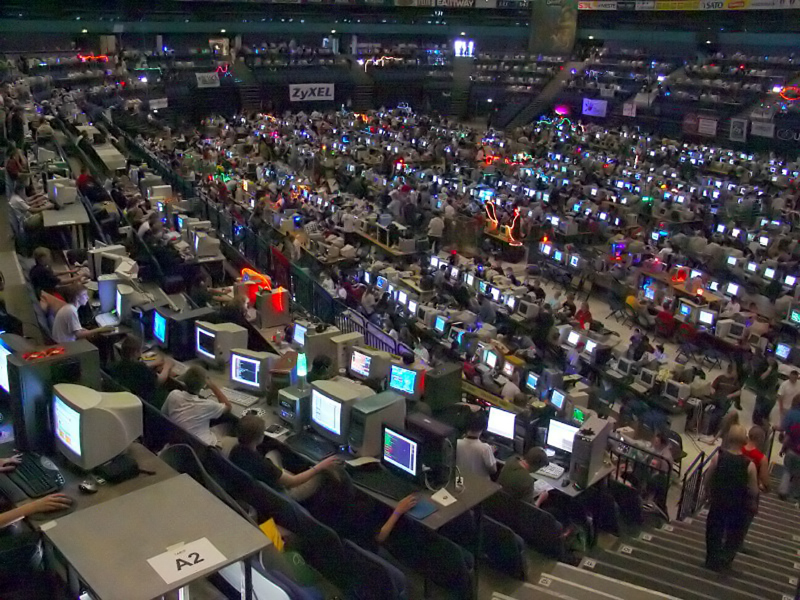
\includegraphics[width=10cm]{archivos/Assembly2004}
	\caption{Assembly 2004 - Fuente: \href{https://en.wikipedia.org/wiki/Demoscene\#/media/File:Assembly2004-areena01.jpg}{Wikipedia}}
	\label{fig:assembly}
\end{figure}

\section{Grupos de demoscening}

A continuación se listan y describen brevemente algunos de los grupos de \emph{demosceners} más populares.

\subsection{Farbrausch}

Farbraush es un grupo de \emph{demosceners} de origen alemán que empezó a ser notado a partir de diciembre del 2000, con su octava producción, llamada \emph{fr-08: .the .product}\footnote{\url{http://www.farbrausch.de/prod&which=17.py}}.\\

El nombre del grupo se puede traducir como "éxtasis de color". Todos sus proyectos empiezan por "fr-número\_del\_proyecto", donde el número del proyecto se decide en el momento de empezar a trabajar en el mismo, independientemente de cuándo se produzca su lanzamiento.\\

Farbraush tiene un gran cantidad de demos notorias, como Debris [\ref{fig:debris}], que está considerada en el popular portal \emph{demoscener} \url{http://www.pouet.net} como la mejor demo de todos los tiempos.

\begin{figure}[h]
	\centering
	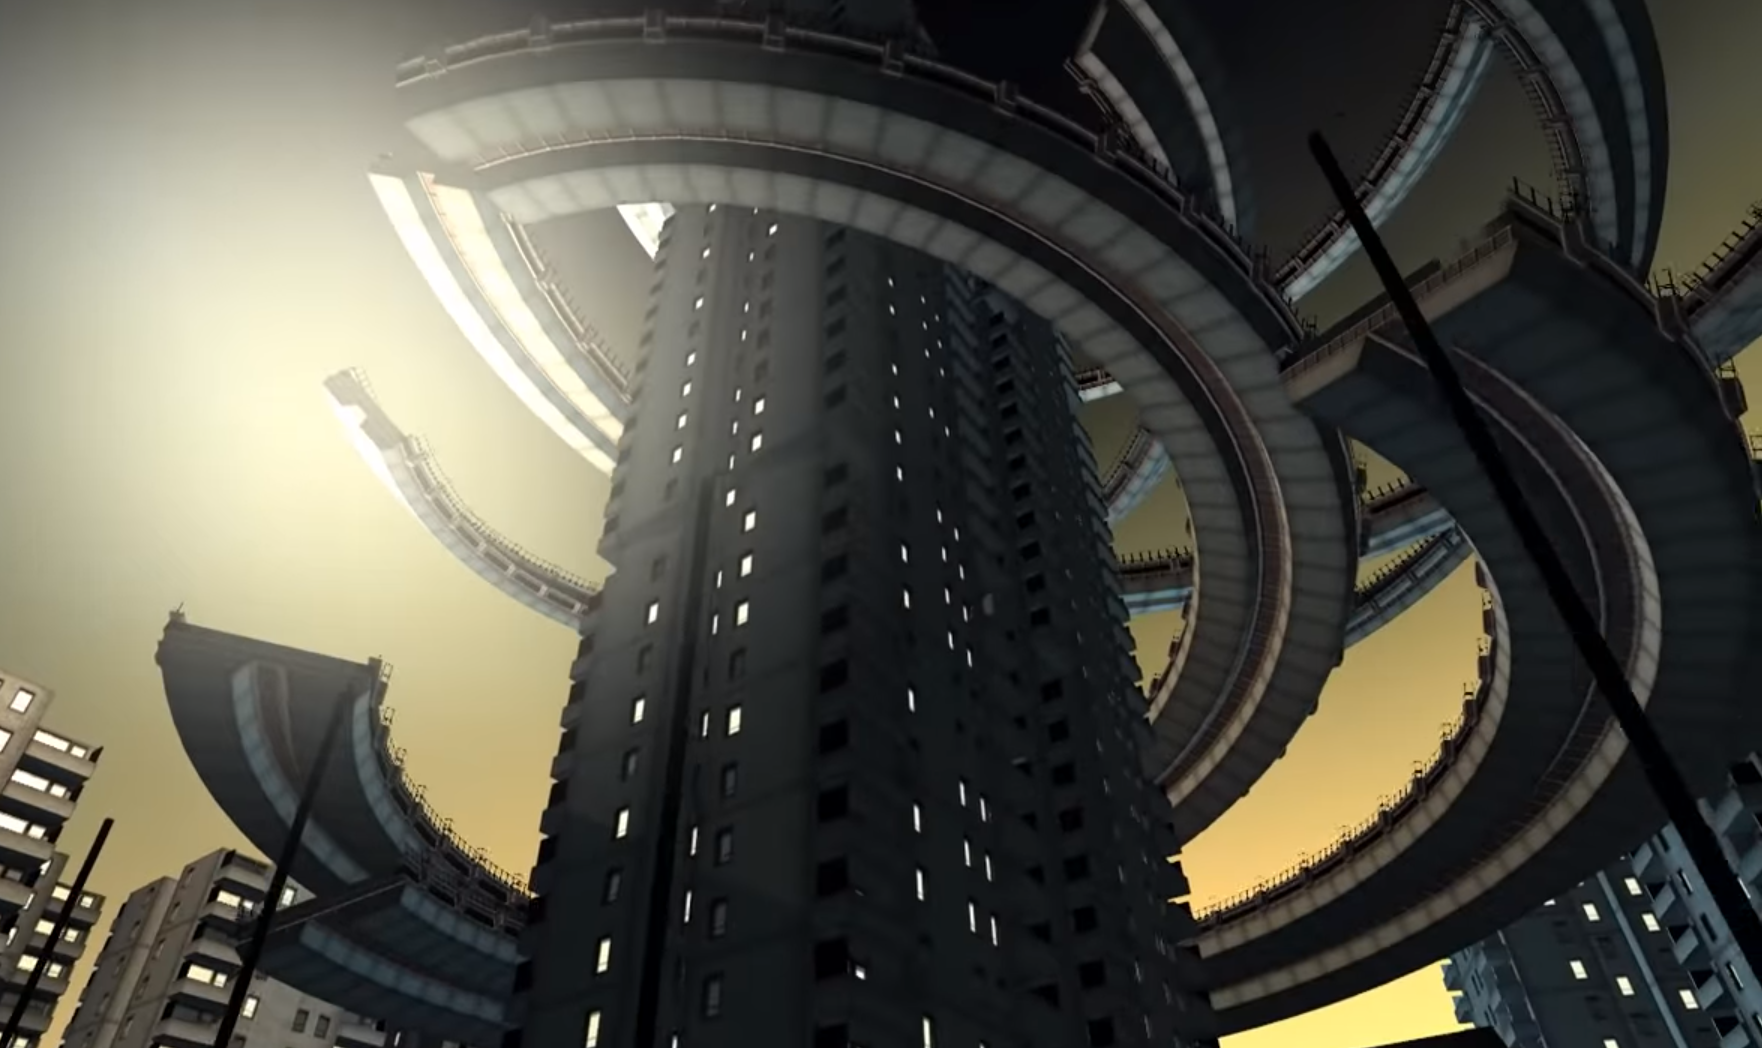
\includegraphics[width=10cm]{archivos/fr-041-debris}
	\caption{Farbrausch 41: Debris - Fuente: \href{https://www.youtube.com/watch?v=jY5Vrc5G0lk}{YouTube}}
	\label{fig:debris}
\end{figure}

Además, en el año 2004 un subgrupo dentro de Farbrausch, denominado \emph{.theprodukkt}, lanzó \emph{.kkrieger}, un juego de disparos en primera persona que ocupaba tan sólo 96kB. Este pequeño tamaño se consiguió mediante el uso de generación procedimental para las texturas y el uso de formas básicas (cubos, esferas...) combinados y deformados para los modelos. El juego [\ref{fig:kkrieger}] recibió distintos premios y fue alabado por la comunidad.\\

\begin{figure}[h]
	\centering
	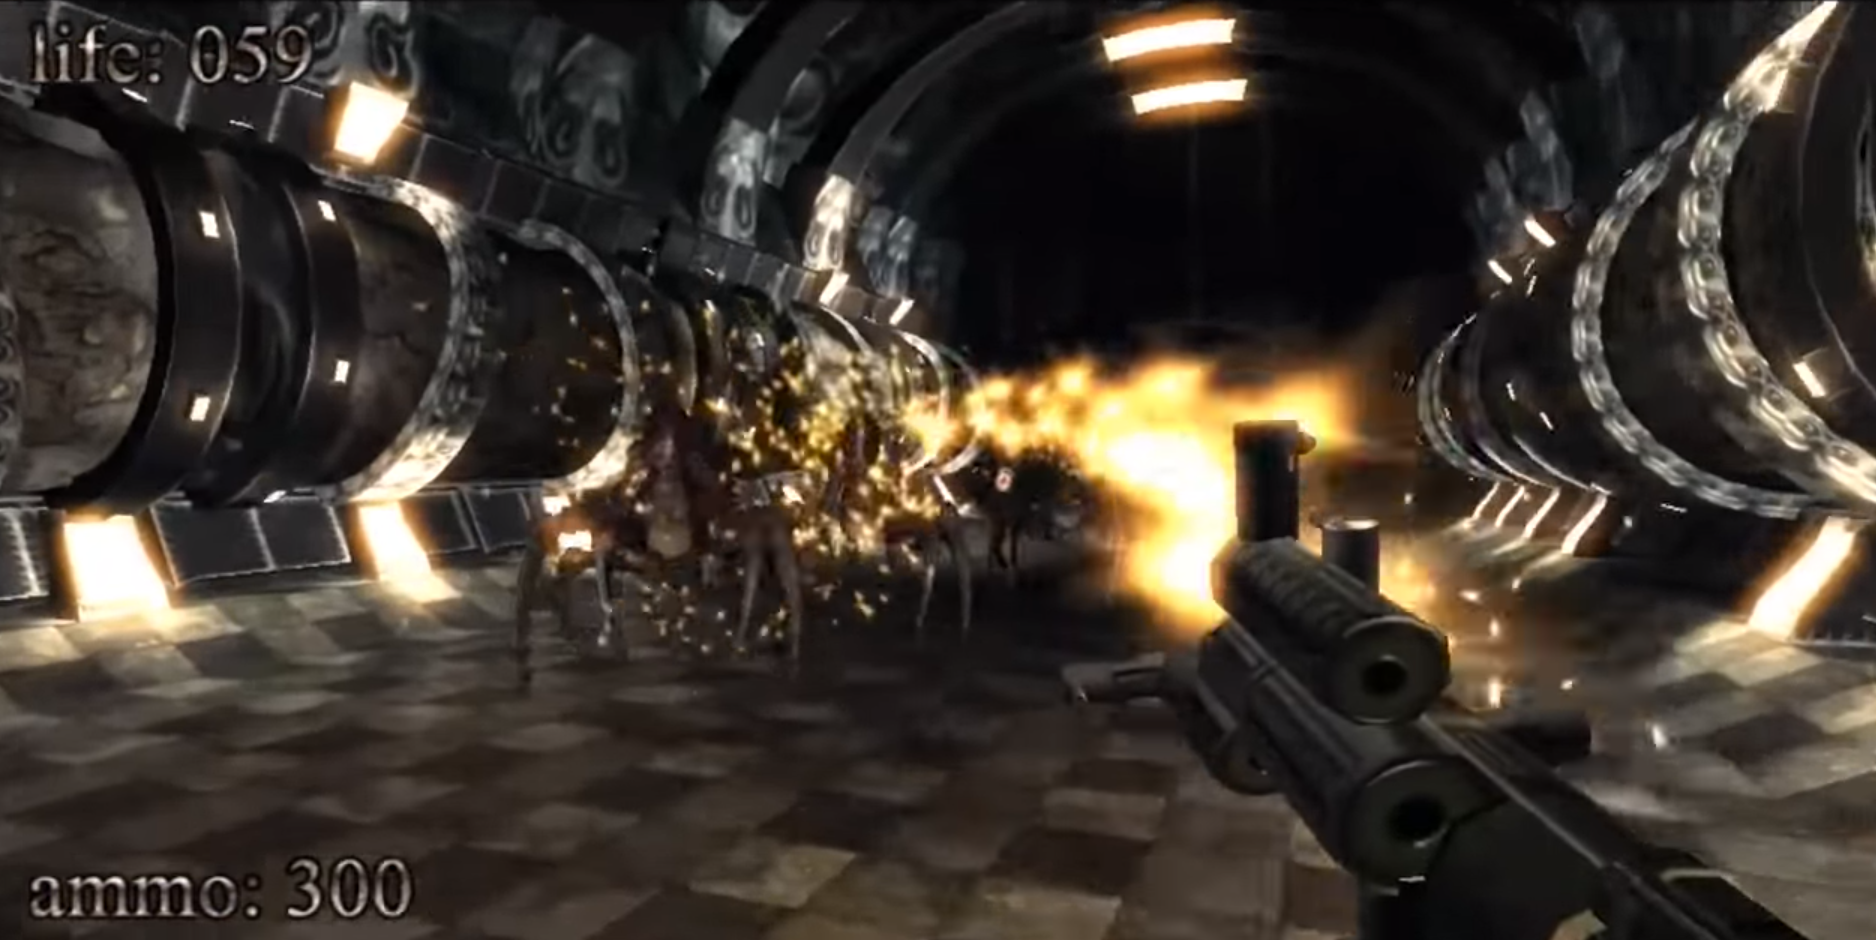
\includegraphics[width=10cm]{archivos/kkrieger}
	\caption{Videojuego de 96kB: .kkrieger - Fuente: \href{https://www.youtube.com/watch?v=2NBG-sKFaB0}{YouTube}}
	\label{fig:kkrieger}
\end{figure}

El grupo sigue en activo y siguen produciendo obras de gran calidad, contando con más de diez productos que han recibido primeros premios en distintas competiciones. En general, sus demos tienden a proseer una temática bastante urbana o robótica, con un cierto aire post-apocalíptico.
Sin embargo, su capacidad, imaginación y variedad de contenido [\ref{fig:magellan}] nunca deja de sorprender.

\begin{figure}[h]
	\centering
	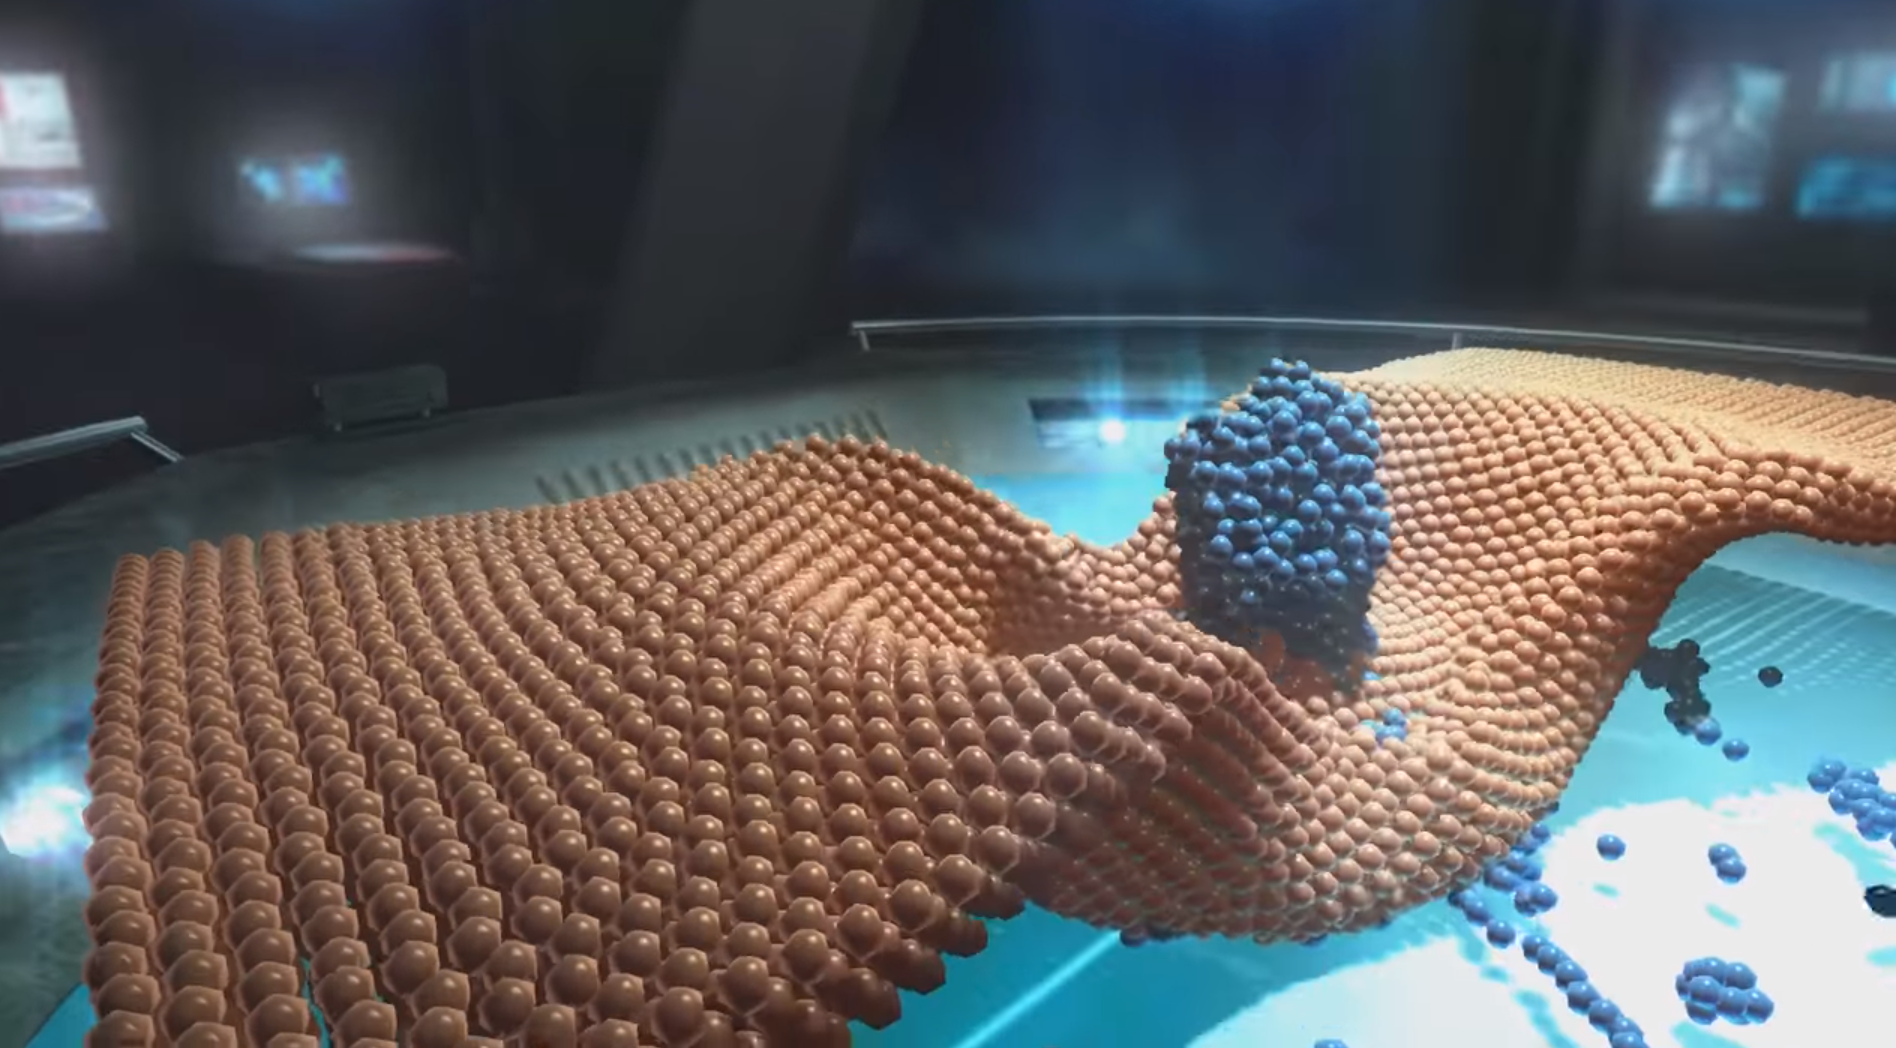
\includegraphics[width=10cm]{archivos/fr-063-magellan}
	\caption{Farbrausch 63: Magellan - Fuente: \href{https://www.youtube.com/watch?v=2Vguvli1Y0k}{YouTube}}
	\label{fig:magellan}
\end{figure}

\subsection{Future Crew}

Future Crew\footnote{\url{https://en.wikipedia.org/wiki/Future_Crew}} fue un grupo de \emph{demosceners} finés, activo principalmente entre 1987 y 1994. Su obra y legado son ampliamente conocidos en el mundo de la \emph{demoscene}. El grupo empezó creando demos para Commodore 64, aunque no tardó en pasar a PC.\\

Su trabajo es especialmente conocido no sólo por su calidad, si no también porque consiguieron resultados que en aquella época parecían imposibles. Su demo, Second Reality [\ref{fig:secondreality}], publicada en julio de 1993, se considera una de las demos más influyentes en la historia de la \emph{demoscene}. Además, el grupo fue coorganizador de la primera edición de la \emph{demoparty} Assembly.\\

\begin{figure}[h]
	\centering
	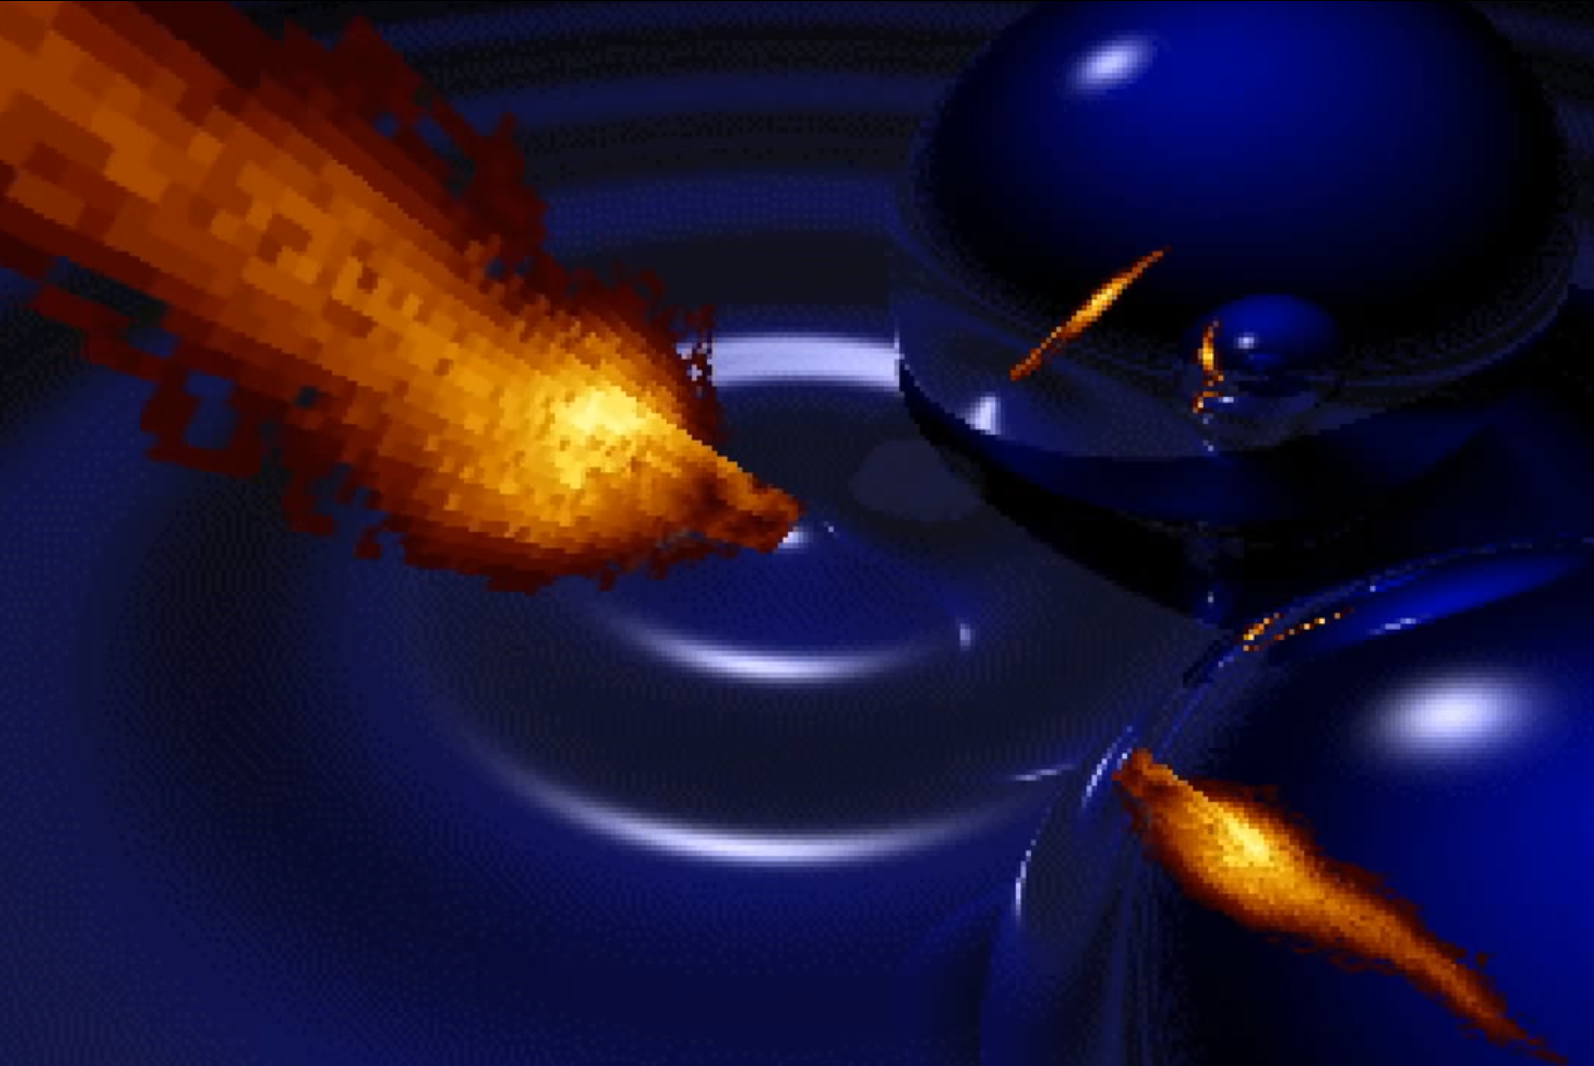
\includegraphics[width=10cm]{archivos/second-reality}
	\caption{Second Reality - Fuente: \href{https://www.youtube.com/watch?v=XezcZVu66QI}{YouTube} - En esta captura se puede ver un efecto de reflexión en dos esferas en tiempo real, mediante \emph{raytracing}}
	\label{fig:secondreality}
\end{figure}

Si bien no se produjo una disolución oficial, el grupo se fue deshaciendo paulatinamente hacia la segunda parte de los 90. La mayoría de sus miembros pasaron a la industria del videojuego o de los gráficos por computador, muchos de ellos fundando sus propios estudios, con resultados exitosos.

\subsection{PoPsY TeAm}

PoPsY TeAm\footnote{\url{http://www.popsyteam.org}} es un grupo de \emph{demosceners} franceses fundado en Lyon, en julio de 1996. Empezaron produciendo demos para Atari y posteriormente para PC.\\

Son los creadores y promotores de VIP (Very Important Party), la \emph{demoparty} más relevante de Francia. Además, PoPsY TeAm se estableció en 2001 como una asociación legalmente registrada en Francia.\\

Su demo más conocida es VIP2 [\ref{fig:vip2}], una demo que presentaron en la \emph{demoparty} holandesa TakeOver en el 2000, resultando ganadora. El objetivo de esta demo era también el de promover su propia \emph{demoparty}, VIP. Esta demo, además, fue la primera de PoPsY TeAm en usar aceleración gráfica por hardware.\\

\begin{figure}[h]
	\centering
	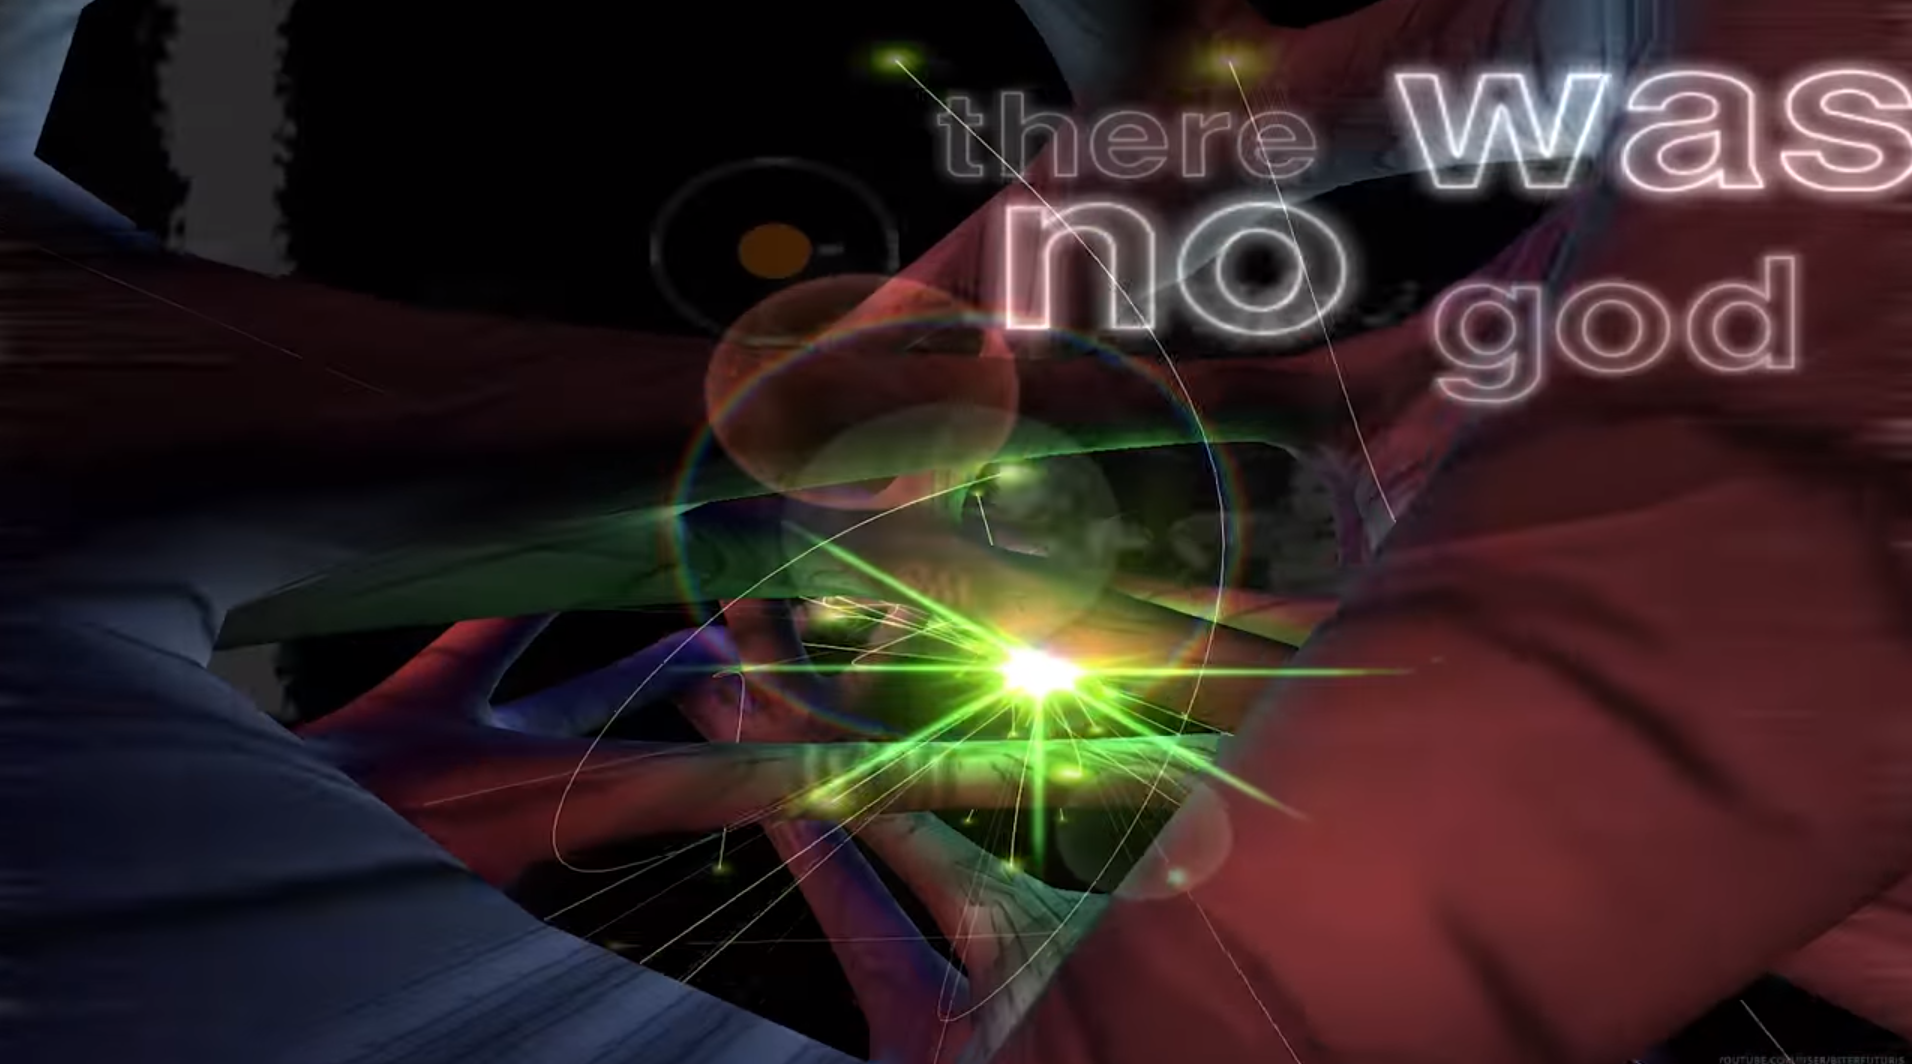
\includegraphics[width=10cm]{archivos/vip2}
	\caption{VIP2 - Fuente: \href{https://www.youtube.com/watch?v=ObtPizPFMbo}{YouTube}}
	\label{fig:vip2}
\end{figure}

El grupo siempre ha intentado promover la \emph{demoscene} y entre otras cosas, han llegado a organizar viajes en bus a diversas partes de Europa para hacer posible al resto de \emph{demosceners} de la región de Lyon atender a \emph{demoparties} europeas. Además, diversos miembros del equipo han participado en la industria del videojuego.

\subsection{Equinox}

Equinox\footnote{\url{https://equinox.planet-d.net}} es un grupo de \emph{demosceners} francés que estuvo principalmente activo entre 1988 y 2007, siendo principalmente conocido por sus demos para Atari ST, aunque sus últimas demos, publicadas pasado el cambio de milenio, fueron lanzadas para PC.

\begin{figure}[h]
	\centering
	\begin{subfigure}[b]{0.45\textwidth}
		\centering
		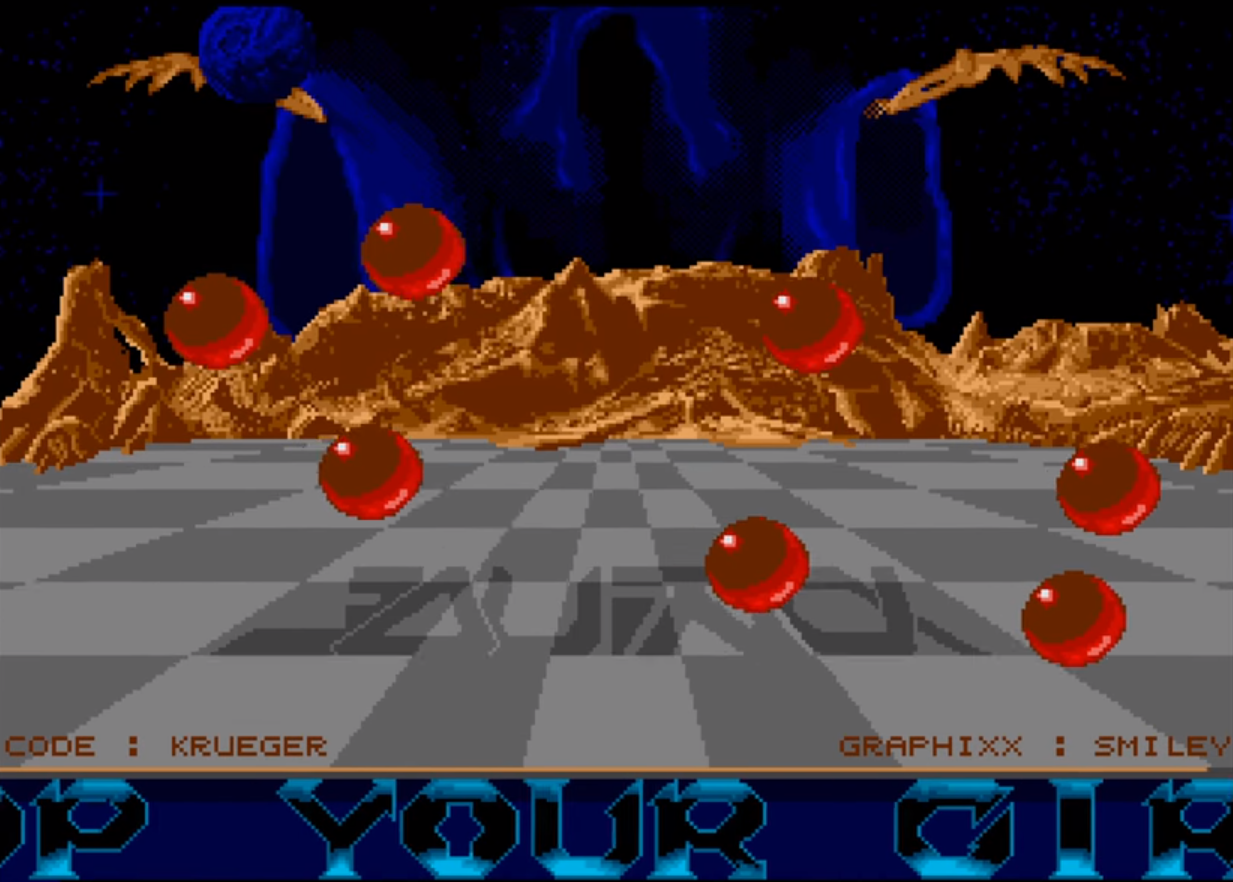
\includegraphics[width=6cm]{archivos/equinox1}
		\caption{Pupul intro (1989) - Fuente : \href{https://www.youtube.com/watch?v=efjEJIj5rhM}{YouTube}}
		\label{fig:equinox1}
	\end{subfigure}
	\begin{subfigure}[b]{0.45\textwidth}
		\centering
		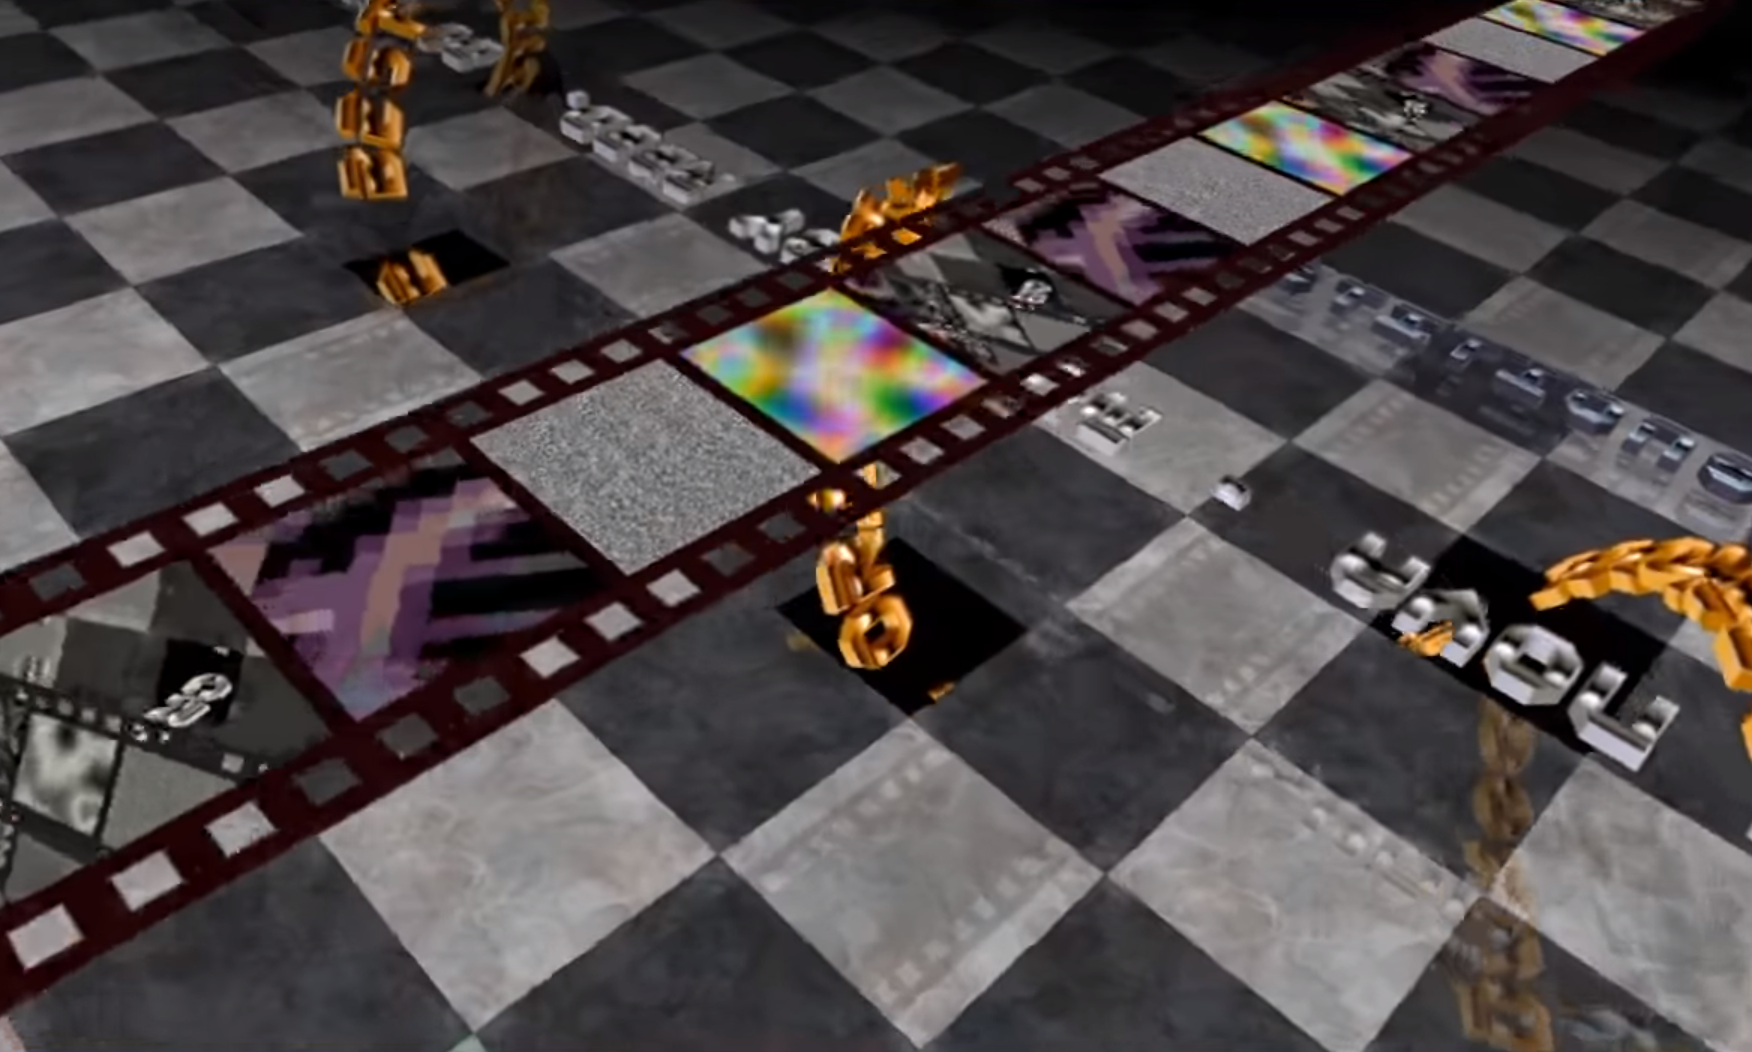
\includegraphics[width=6cm]{archivos/equinox2}
		\caption{Sota 2004 invitation intro (64k intro) - Fuente: \href{https://www.youtube.com/watch?v=cb8i0WYDLxM}{YouTube}}
		\label{fig:equinox2}
	\end{subfigure}
	\label{hace flata}
\end{figure}

\subsection{Fairlight}

FairLight\footnote{\url{http://www.fairlight.to}} es un grupo de \emph{demosceners} de origen sueco, formado en 1987. FairLight empezó creando demos para Commodore, aunque ha creado también demos para Amiga, SNES y posteriormente en PC.\\

FairLight fue fundado en 1987 por dos \emph{crackers} suecos, ex-miembros de un grupo llamado "West Coast Crackers". De hecho, FairLight no solo se dedicaba a la \emph{demoscene}, si no también al mundo del \emph{cracking}, rompiendo juegos para su lanzamiento gratuito de forma ilegal. De hecho, llegaron a hacerse especialmente conocidos por la velocidad a la que eran capaces de lanzar juegos \emph{crackeados}\footnote{\url{https://computersweden.idg.se/2.2683/1.444716/we-might-be-old-but-were-still-the-elite}}. Tal fue su impacto que en Abril de 2004, varios miembros del grupo fueron tomados por el FBI en una operación antipiratería denominada \emph{Operation FastLink}. Más de 120 personas fueron arrestadas en esta operación, en la que se consideraba a los \emph{crackers} como una organización criminal.\\

\begin{figure}[h]
	\centering
	
\includegraphics[width=10cm]{archivos/fairlight}
	\caption{Dead Ringer (por FairLight) - Fuente: \href{https://www.youtube.com/watch?v=Mc_TR4mcJKE}{YouTube} - Demo 64k ganadora de Assembly 2006}
	\label{fig:fairlight}
\end{figure}

Este es, quizás, un grupo en el que se reflejan y mezclan los orígenes de la \emph{demoscene}, provenientes del mundo del \emph{cracking}. A pesar de todo, el grupo volvió a estar en activo a partir de octubre de 2006.

\subsection{RGBA}

RGBA\footnote{\url{http://www.rgba.org}} es un grupo español de \emph{demosceners} que estuvo activo entre 2001 y 2009. Todas sus producciones fueron lanzadas para PC, principalmente en Windows.\\

Son especialmente conocidos por su demo Elevated[\ref{fig:elevated}]. Esta demo, realizada en colaboración con TBC\footnote{\url{https://demozoo.org/groups/641/}}, es especialmente conocida y celebrada por la comunidad \emph{demoscener}, situándose como la segunda más popular en el portal \url{http://www.pouet.net}.\\

Los binarios de todas sus producciones se pueden encontrar en \href{https://github.com/reality3d/rgba-prods}{GitHub}.\\

\begin{figure}[h]
	\centering
	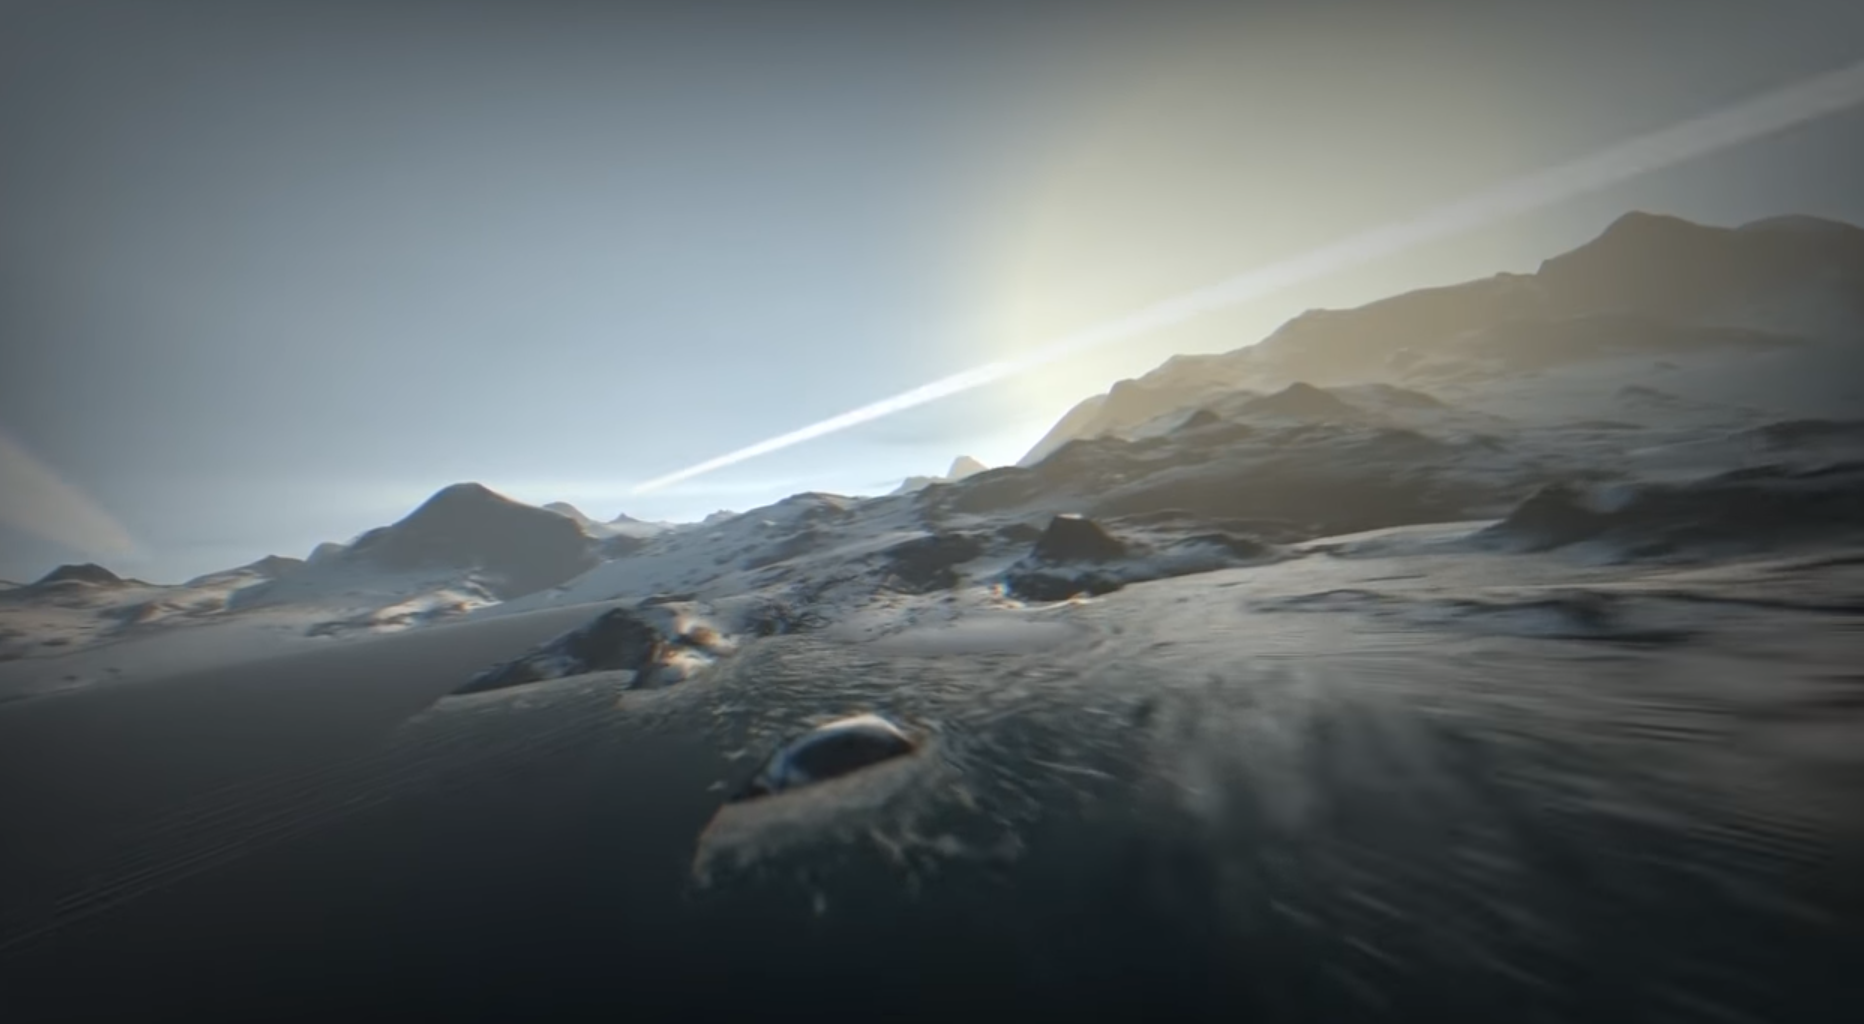
\includegraphics[width=10cm]{archivos/elevated}
	\caption{Elevated - Fuente: \href{https://www.youtube.com/watch?v=jB0vBmiTr6o}{YouTube} - Intro 4K ganadora en Breakpoint 2009}
	\label{fig:elevated}
\end{figure}

\subsection{Batman Group}

Batman Group\footnote{\url{https://demozoo.org/groups/18871/}} es un modesto grupo de \emph{demosceners} de origen español, activo desde 1993. Han producido juegos y demos para Amstrad CPC, ZX Spectrum, Amiga, Android e iOS.\\

Su demo más conocida es Batman Forever[\ref{fig:batmanforever}], para Amstrad CPC, lanzada en 2011 para la \emph{demoparty} eslovaca Forever, quedando en primera posición.\\

\begin{figure}[h]
	\centering
	
\includegraphics[width=10cm]{archivos/batmanforever}
	\caption{Batman Forever - Fuente: \href{https://www.youtube.com/watch?v=dqjZNnjNu3Y}{YouTube}}
	\label{fig:batmanforever}
\end{figure}

El grupo se vio envuelto en una polémica a finales de 2018, debido a que el grupo de desarrolladores retro \emph{4MHz} había usado para sus producciones código cedido por Batman Group sin su correcta atribución. La polémica se resolvió con la disolución de todo tipo de relación entre Batman Group y 4MHz\footnote{\url{http://www.amstrad.es/forum/viewtopic.php?t=5247}}.

\section{Portales de demoscening}
Hablar de pouet especificamente y luego del alguna más

\section{Demos destacables}
juntar y hablar de las principales demos en la demoscene, hacer referencia al top de pouet, incluir elevated y otras mas e intentar explicarlas

\section{Efectos gráficos más comunes}
comentar algunos de los efectos de la demoscene más comunes y cómo se conseguían (comentar cómo se conseguían sólo por encima)

%http://www.farbrausch.de/index.py https://en.wikipedia.org/wiki/Farbrausch
%https://en.wikipedia.org/wiki/Future_Crew https://demozoo.org/groups/357/
%http://www.popsyteam.org https://en.wikipedia.org/wiki/Very_Important_Party
%https://en.wikipedia.org/wiki/Equinox_(Atari_demogroup) https://equinox.planet-d.net/atari.html
%https://demozoo.org/groups/18871/
%https://en.wikipedia.org/wiki/Fairlight_(group)

\section{Influencia de la demoscene en la industria}

La \emph{demoscene} siempre se ha mantenido de forma discreta. Algunas de las razones de que esto sea así se han listado anteriormente, como el hecho de que hace una gran cantidad de conocimiento y pasión para poder participar de forma activa en ella. Sin embargo, esto no ha impedido dejar su huella en la industria informática, especialmente en la del videojuego.\\

La lista de personalidades que vienen del mundo de la \emph{demoscene} o se han visto influidos por ella es extensa\footnote{\url{https://chipflip.wordpress.com/2015/06/12/famous-people-who-came-from-the-demoscene/}}. A continuación se listan algunas de las más destacables:

\begin{itemize}
	\item \textbf{DICE}\footnote{\url{http://www.dice.se}}: La compañía \emph{Digital Illusions}, conocida por juegos como varios de los títulos de la saga \emph{Battefield} o \emph{Mirror's Edge Catalyst}, cuenta con una gran plantilla proveniente de la \emph{demoscene}, entre los que podemos contar miembros de FairLight.
	\item \textbf{Remedy}\footnote{\url{https://www.remedygames.com/}}: Esta compañía es especialmente conocida por la saga Max Payne. Fue cofundada por dos miembros de Future Crew. Además, esta compañía mantenía una estrecha relación con Futuremark, creadores de 3DMark, un software de pruebas de rendimiento (\emph{benchmarks}). Esta última compañía también poseía una gran cantidad de miembros provenientes de la \emph{demoscene}, contando con varios de Future Crew.
	\item \textbf{Starbreeze, Ascaron, 49Games, Techland, Lionhead Studios, Guerrilla Games}: Todas estas compañías también cuentan o han contado con miembros de la \emph{demoscene}.
	\item Will Wright, creador del vieojuego Spore, afirma que la \emph{demoscene} fue una gran influencia para al juego, debido a que este está fundamentalmente basado en la generación procedimental de contenido\footnote{\url{http://www.gamespy.com/articles/595/595975p1.html}}.
	\item John Carmack, \emph{lead programmer} de videojuegos como Wolfestein 3D, Doom y Quake, afirmó en la QuakeCon de 2011 que tiene en alta consideración a aquellos programadores que desarrollan demos de 64K, pues tienen que hacer frente a grandes limitaciones y se obtiene mucho conocimiento en el proceso\footnote{\url{https://www.youtube.com/watch?v=4zgYG-_ha28\#t=4827s}}.
	\item Jaakko Iisalo, principal diseñador de Angry Birds, fue un \emph{demoscener} activo y reconocido durante los 90.
\end{itemize}

Además, hay algunas otras subculturas informáticas que están estrechamente relacionadas con la \emph{demoscene} o derivan de la misma, como por ejemplo la música por \emph{tracker} (hay toda una comunidad de músicos que crean producciones a través del uso de \emph{trackers}, software para la producción de música).

%Importantes para la historia:
%http://widerscreen.fi/assets/reunanen-wider-1-2-2014.pdf
%http://www.oldskool.org/demos/explained/demo_history.html
%https://web.archive.org/web/20170726063815/http://tomaes.32x.de/text/faq.php#2.3.

%Elevated y otras demos por el estilo

%https://web.archive.org/web/20170726063815/http://tomaes.32x.de/text/faq.php
%http://www.oldskool.org/demos/explained/demo_history.html

%http://www.oldskool.org/demos/explained/demo_reference.html

%http://www.demoscene.info
%http://www.pouet.net/index.php
%https://en.wikipedia.org/wiki/Assembly_(demoparty)
%https://en.wikipedia.org/wiki/Demoscene

%http://widerscreen.fi/numerot/2014-1-2/crackers-became-us-demosceners/
%http://www.oldskool.org/demos/explained/demo_pages.html
%ftp://ftp.hornet.org/pub/demos/info/demonews/1998/demonews.150

%http://www.farbrausch.de/index.py 
%https://en.wikipedia.org/wiki/Farbrausch
%https://en.wikipedia.org/wiki/Future_Crew 
%https://demozoo.org/groups/357/
%http://www.popsyteam.org 
%https://en.wikipedia.org/wiki/Very_Important_Party
%https://en.wikipedia.org/wiki/Equinox_(Atari_demogroup) 
%https://equinox.planet-d.net/atari.html
%https://demozoo.org/groups/18871/	% Plantilla: Se muestran listas
%%%%%%%%%%%%%%%%%%%%%%%%%%%%%%%%%%%%%%%%%%%%%%%%%%%%%%%%%%%%%%%%%%%%%%%%
% Plantilla TFG/TFM
% Escuela Politécnica Superior de la Universidad de Alicante
% Realizado por: Jose Manuel Requena Plens
% Contacto: info@jmrplens.com / Telegram:@jmrplens
%%%%%%%%%%%%%%%%%%%%%%%%%%%%%%%%%%%%%%%%%%%%%%%%%%%%%%%%%%%%%%%%%%%%%%%%

\chapter{Objetivos}

Aprender el bajo nivel y rendimiento, crear varios efectos básicos, crear un efecto más complejo		% Plantilla: Se muestran tablas
%%%%%%%%%%%%%%%%%%%%%%%%%%%%%%%%%%%%%%%%%%%%%%%%%%%%%%%%%%%%%%%%%%%%%%%%
% Plantilla TFG/TFM
% Escuela Politécnica Superior de la Universidad de Alicante
% Realizado por: Jose Manuel Requena Plens
% Contacto: info@jmrplens.com / Telegram:@jmrplens
%%%%%%%%%%%%%%%%%%%%%%%%%%%%%%%%%%%%%%%%%%%%%%%%%%%%%%%%%%%%%%%%%%%%%%%%

\chapter{Metodología}

\section{Software}

\begin{itemize}
	\item \textbf{Toggle}\footnote{\url{https://toggl.com/}}: Se utilizará la herramienta online Toggl para contabilizar el tiempo dedicado a cada parte del proyecto. Esto permitirá poder analizar qué partes del trabajo han requerido más dedicación y por qué, ayudando a completar el estudio.
	\item \textbf{Git}\footnote{\url{https://git-scm.com}}: Se utilizará Git para el control de versiones. El uso de Git nos permitirá, además, tener un registro detallado de la evolución del código. El código para este proyecto se aloja en GitHub\footnote{\url{https://github.com/donluispanis/TFG}}.
	\item \textbf{Make}\footnote{\url{https://www.gnu.org/software/make/}}: El código de este proyecto será compilable tanto en las plataformas Windows como Linux. Para ello, el uso de la herramienta Make facilitará la compilación de los proyectos así como su portabilidad.
	\item \textbf{MinGW}\footnote{\url{http://www.mingw.org}}: MinGW es un entorno de desarrollo para Windows que ofrece un entorno similar al de GNU. Se usará para compilar tanto el código como las librerías en Windows, haciendo la portabilidad más consistente y sencilla.
	\item \textbf{GCC}\footnote{\url{https://gcc.gnu.org}}: GCC es una colección de compiladores con soporte para C++. Se usará para compilar el código de este proyecto, tanto en Windows (a través de MinGW) como en Linux (de forma nativa).
	\item \textbf{GLFW}\footnote{\url{https://www.glfw.org}}: GLFW es una librería multiplataforma para OpenGL que facilita los procesos de creación de ventana, generación de contexto y manejo de input. 
	\item \textbf{OpenGL}\footnote{\url{https://www.opengl.org}}: OpenGL es una extendida librería para la creación y manipulación de gráficos bidimensionales y tridimensionales. En este proyecto, sin embargo, su uso será mínimo y restringido. Se utilizará tan solo para dibujar una textura en nuestra ventana. Será mediante la manipulación de esta textura que generaremos gráficos. OpenGL, por tanto, será un mero mediador, redibujando constantemente la misma textura en pantalla.
	\item \textbf{Valgrind}\footnote{\url{http://valgrind.org}}: Valgrind es una herramienta de depuración y perfilado. Se utilizará para realizar pruebas de rendimiento y para comprobar el correcto funcionamiento del programa. 
	\item \textbf{Compiler Explorer}\footnote{\url{https://godbolt.org}}: Compiler Explorer es una herramienta online que permite ver la salida en ensamblador del código escrito de forma instantánea. Resultará muy útil para analizar y entender mejor el código que se ejecuta.
\end{itemize}

\section{Tests de rendimiento}

Se pretende recopilar una serie de resultados cuantificables que muestren el coste de distintos tipos de operaciones computacionales, tanto a nivel de coste temporal como espacial (y cantidad de instrucciones).\\

Se realizará un análisis exhaustivo de los resultados obtenidos, exponiéndolos y razonando acerca de los mismos.\\

Para realizar estas pruebas, se procederá a la ejecución de pequeños programas que contengan pruebas concretas. Las pruebas que se propone realizar son: operaciones matemáticas con números enteros, operaciones matemáticas con números en coma flotante, coste de la reserva y liberación de memoria, coste del acceso a memoria y coste de los bucles y las operaciones condicionales.\\

Tras analizar los resultados, se elaborarán una serie de directrices para escribir código que sea generalmente más rápido y/o más fácilmente optimizable por el compilador. Para poder analizar correctamente los resultados obtenidos, se tendrá en cuenta el código ensamblador generado por el compilador.\\

\section{Entorno: motor gráfico}

El objetivo final de este proyecto es recopilar e implementar una serie de efectos gráficos. Sin embargo, para poder realizar esta tarea, es necesario disponer de un entorno que nos permita realizar labores básicas, como gestión de la ventana o de input.\\

Mediante la creación de un entorno se asegura un flujo de trabajo consistente entre todas las demos, así como la reutilización de código. Será necesaria, por tanto, la creación de un motor gráfico. Este motor deberá de ser lo más sencillo posible, pues debe limitarse a facilitar tareas básicas, pero no debe ofrecer soluciones a problemas complejos o específicos a una demo. Este motor debe ser conciso y ligero, pues debe influir lo mínimo posible en el rendimiento de la demo.\\

Este motor debe darnos soporte para: manejo de la ventana, acceso a un espacio de memoria donde sea posible manipular gráficos, manejo de entradas de teclado, dibujado básico en ventana (puntos, líneas, areas rectangulares y texto)

\section{Las demos}

Para afrontar cada una de las demos, se seguirá un procedimiento común que se expone a continuación.

\subsection{Búsqueda de información}

En una primera fase, se procederá a la búsqueda de documentación e información sobre la demo. Esto incluye tanto vídeos como imágenes, además de tutoriales o explicaciones teóricas. En esta fase, se plantea recopilar tanta información acerca de la demo como sea posible, y lograr un modelo teórico básico acerca de cómo debería funcionar.

\subsection{Planteamiento formal}

Una vez se ha recopilado información sobre la demo a estudio y se posee un conocimiento suficiente sobre la misma, se procede a un planteamiento formal, previo a su implementación. Este planteamiento incluye entender en profundidad la base matemática de la demo, si la hay. Se debe realizar un análisis y explorar distintos puntos de vista desde los que se podría implementar la demo.

\subsection{Implementación}

Analizada la demo, y se habiendo razonado sobre el mejor modo de desarrollarla, se procede a la fase de implementación en código de la demo. Esta es una fase experimental y que permite flexibilidad. Es posible que sea necesario probar distintos acercamientos, buscando el que más se adecúe al resultado que se busca y que ha sido definido en el planteamiento formal de la demo.

\subsection{Refinamiento}

Cuando la demo ya está completada a nivel de funcionalidad, se procede a su refinamiento y refactorización. En esta fase se busca hacer el código más legible (nombres de variables y funciones explícitos, correcta documentación del código...) así como hacer el código más eficiente (identificar los factores críticos del programa y buscar e implementar soluciones más eficientes).	% Plantilla: Se muestran figuras
\chapter{Tests de rendimiento}

\section{Planteamiento inicial}

Siguiendo el carácter definido previamente, el objetivo de este trabajo es poder hacerlo todo desde cero, en la medida de lo que resulta posible o razonable.\\

Es por ello, que siguiendo este mismo espíritu busqué crear mi propio marco de trabajo para ejecutar pequeños tests de rendimiento. Esto es todo lo que debería ser capaz de hacer mi herramienta:

\begin{itemize}
	\item Ser capaz de ejecutar un test provisto de forma externa
	\item Ejecutar cada test múltiples veces, para poder obtener un abanico de tiempos de ejecución
	\item Extraer una media de los resultados obtenidos en la medición
	\item Mostrar los resultados obtenidos por terminal, así como almacenarlos en un fichero de texto
\end{itemize}

Al ser pocos los requerimientos de mi herramienta, el desarrollo de la misma debería ser breve y sencillo.\\

Además, llegó también el momento de plantear el carácter los tests a realizar:

\begin{itemize}
	\item Medir el coste de la suma, resta, multiplicación, división y módulo para enteros de 32 bits
	\item Medir el coste de la suma, resta, multiplicación, división y módulo para enteros de 64 bits
	\item Medir el coste de la suma, resta, multiplicación y división para números en coma flotante de 32 bits
	\item Medir el coste de la suma, resta, multiplicación y división para números en coma flotante de 64 bits
	\item Medir el coste de llamar a una función generadora de números aleatorios, llamar una función de coseno, de arco coseno, de raíz cuadrada y de raíz cúbica en comparación al coste de llamar a una función vacía
	\item Medir el coste de acceso aleatorio a memoria
	\item Medir el coste de acceso directo o indirecto a memoria
\end{itemize}

\section{Implementación}

Para inicializar la clase que manejará nuestros tests, debemos crearla pasándole por parámetro una cadena de caracteres que represente la ruta del fichero donde queremos que se guarde el resultado de nuestros tests. Tras mostrar por terminal un código de "bienvenida", abrimos el fichero con la ruta especificada y, a continuación, inicializamos dos \emph{buffers}. Será redirigiendo la salida de \lstinline{std::cout} a cada uno de estos \emph{buffers} como conseguiremos escribir tanto en terminal como en fichero.

\begin{lstlisting}[style=C-color, caption={Constructor de nuestra clase para manejar tests}, label=cod:testtemplate, escapechar=|]
TestTemplate::TestTemplate(const char *logPath)
{
    std::cout << std::endl;
    std::cout << "Running tests... this may take a while" << std::endl;
    std::cout << "Output will be stored in " << logPath << std::endl;
    std::cout << std::endl;

    file = std::ofstream(logPath);
    writeToScreen = std::cout.rdbuf();
    writeToFile = file.rdbuf();
}
\end{lstlisting}

A continuación, llega el momento de crear un método que nos permita ejecutar nuestros tests, como podemos ver en el código [\ref{cod:executetest}]. Este método recibe una función por parámetro, que ejecutará internamente 100 veces el test pasado,  y almacenará el tiempo de cada ejecución en un vector.

\begin{lstlisting}[style=C-color, caption={Método para ejecutar un test}, label=cod:executetest, escapechar=|]
void TestTemplate::ExecuteTest(std::function<void(void)> test)
{
    timeCounts.clear();
    std::chrono::duration<double> elapsedSeconds;

    for (int i = 0; i < 100; i++)
    {
        time_point = std::chrono::system_clock::now();

        test();

        elapsedSeconds = std::chrono::system_clock::now() - time_point;
        timeCounts.push_back(elapsedSeconds.count());
    }
}
\end{lstlisting}

Será entonces, tras haber ejecutado nuestro test, que podremos obtener el tiempo medio de ejecución con el siguiente código:

\begin{lstlisting}[style=C-color, caption={Método para calcular la media del tiempo transcurrido}, label=cod:calculatetime, escapechar=|]
double TestTemplate::CalculateAverageTime()
{
    double time = std::accumulate(timeCounts.begin(), timeCounts.end(), 0.0) / (double)timeCounts.size();
    return time;
}
\end{lstlisting}

Proveeremos además con un método [\ref{cod:writeresults}] que dado el nombre del test, una descripción del mismo y el tiempo que ha tardado en ejecutarse, escribe de forma fácilmente legible para el ojo humano los resultados de la ejecución. El resultado se escribe tanto en fichero como por terminal, redirigiendo la salida de texto.

\begin{lstlisting}[style=C-color, caption={Método para calcular la media del tiempo transcurrido}, label=cod:writeresults]
void TestTemplate::WriteTestResultsIntoScreenAndFile(const char *testName, const char *testDescription, double testTime)
{
    auto output = [](const char *testName, const char *testDescription, double testTime) {
        std::cout << "| Test " << testName << ": " << testDescription << std::endl;
        std::cout << "|          Time spent: " << testTime << " seconds" << std::endl;
        std::cout << "|" << std::endl;
    };

    std::cout.rdbuf(writeToFile);
    output(testName, testDescription, testTime);

    std::cout.rdbuf(writeToScreen);
    output(testName, testDescription, testTime);
}
\end{lstlisting}

Tal vez lo mostrado hasta ahora pueda parecer un poco confuso, pero es al combinar todo este código para ejecutar un test cuando se ve la potencia de la clase que hemos creado, que nos permite manejar tests con facilidad, de forma legible y sencilla:

\begin{lstlisting}[style=C-color, caption={Ejemplo de uso de test template}, label=cod:example]
TestTemplate T("PerformanceResults.txt");

T.ExecuteTest([]() {for (int j = 0; j < 10000000; j++); });
T.WriteTestResultsIntoScreenAndFile("Loops", "Void For Loop executed 10000000 times", T.CalculateAverageTime());
\end{lstlisting}

\begin{lstlisting}[caption={Resultado del test}, label=cod:exampleresult]
| Test Loops: Void For Loop executed 10000000 times
| Time spent: 0.0168712 seconds
|
\end{lstlisting}

El test de ejemplo mostrado en el código [\ref{cod:example}] es bastante trivial, pues es un código que se limita a ejecutar un bucle. No obstante, se ejemplifica lo sencillo y limpio que se vuelve escribir un test, con un resultado también fácil de leer e interpretar [\ref{cod:exampleresult}].

\section{Resultados}

El resultado de cada test que se muestra a continuación ha sido hallado a partir de la media de 5 ejecuciones individuales de cada conjunto de tests para cada plataforma. A su vez, cada conjunto de tests ha sido ejecutado internamente un total de 100 veces, como podemos ver en [\ref{cod:executetest}], habiéndose hallado la media de tiempo de estas ejecuciones.\\

Los resultados que se muestran en la columna izquierda vienen dados en segundos, siendo el tiempo de ejecución medio del test. Los resultados que se muestran a la derecha son el resultado ponderado con respecto a un resultado base (por ejemplo, cúantas veces es más costosa una división que una suma).\\

Cada conjunto de tests ha sido compilado a su vez con tres objetivos distintos, siendo estos:

\begin{itemize}
	\item Ejecutable de \textbf{Windows x86} compilado con \textbf{g++ 7.4.0} para \textbf{MinGW32}
	\item Ejecutable de \textbf{Windows x64} compilado con \textbf{g++ 8.2.1} para \textbf{MinGW64}
	\item Ejecutable de \textbf{Linux x64} compilado con \textbf{g++ 8.2.1}
\end{itemize}

Los tests han sido ejecutados en los siguientes sistemas operativos:

\begin{itemize}
	\item \textbf{Windows 10 Home x64} (versión 1803)
	\item \textbf{Manjaro Linux x6}4 (versión 18.0.4)
\end{itemize}

Los tests han sido ejecutados bajo el siguiente hardware:

\begin{itemize}
	\item CPU: \textbf{Intel Core i7-6700HQ} 2.60GHz, x64 processor
	\item RAM: \textbf{16 GB DDR4-2133}
\end{itemize}

Cada operación matemática que se muestra a continuación se ha realizado dentro de un bucle que se ejecuta 10000000 millones de veces, por lo que el resultado que vemos no se debe usar tanto de forma cuantitativa como para establece comparaciones o relaciones.\\

En la tabla [\ref{tab:int32}] se muestran los resultados de realizar operaciones matemáticas con números enteros de 32 bits. En la columna de resultados relativos, se compara el coste de las operaciones con respecto al coste de la suma de enteros de 32 bits.\\

\begin{table}[h]
\centering
\begin{tabular}{@{}l|rrr|rrr|@{}}
\cmidrule(l){2-7}
                                     & \multicolumn{3}{c|}{Results (s)}                                                               & \multicolumn{3}{c|}{Relative results}                                                      \\ \cmidrule(l){2-7} 
                                     & \multicolumn{1}{c|}{Win x86} & \multicolumn{1}{c|}{Win x64} & \multicolumn{1}{c|}{Lin x64} & \multicolumn{1}{c|}{Win x86} & \multicolumn{1}{c|}{Win x64} & \multicolumn{1}{c|}{Lin x64} \\ \midrule
\multicolumn{1}{|l|}{Sum}            & 0,0232331                    & 0,0286147                    & 0,0284548                    & 0,0                          & 0,0                          & 0,0                          \\ \cmidrule(r){1-1}
\multicolumn{1}{|l|}{Subtraction}    & 0,0232895                    & 0,0268971                    & 0,0278414                    & 0,0                          & -0,2                         & -0,1                         \\ \cmidrule(r){1-1}
\multicolumn{1}{|l|}{Multiplication} & 0,0236683                    & 0,0272116                    & 0,0274386                    & 0,1                          & -0,1                         & -0,1                         \\ \cmidrule(r){1-1}
\multicolumn{1}{|l|}{Division}       & 0,0353099                    & 0,0400042                    & 0,0391396                    & 2,7                          & 1,1                          & 1,0                          \\ \cmidrule(r){1-1}
\multicolumn{1}{|l|}{Modulo}         & 0,0361311                    & 0,0392958                    & 0,0451121                    & 2,9                          & 1,0                          & 1,6                          \\ \bottomrule
\end{tabular}
\caption{Operaciones con enteros de 32 bits}
\label{tab:int32}
\end{table}

En la tabla [\ref{tab:int64}] se muestran los resultados de realizar operaciones matemáticas con números enteros de 64 bits. En la columna de resultados relativos, se compara el coste de las operaciones respecto al coste de la suma de enteros de 32 bits.\\

\begin{table}[h]
\centering
\begin{tabular}{@{}l|rrr|rrr|@{}}
\cmidrule(l){2-7}
                                     & \multicolumn{3}{c|}{Results (s)}                                                               & \multicolumn{3}{c|}{Relative results}                                                      \\ \cmidrule(l){2-7} 
                                     & \multicolumn{1}{c|}{Win x86} & \multicolumn{1}{c|}{Win x64} & \multicolumn{1}{c|}{Lin x64} & \multicolumn{1}{c|}{Win x86} & \multicolumn{1}{c|}{Win x64} & \multicolumn{1}{c|}{Lin x64} \\ \midrule
\multicolumn{1}{|l|}{Sum}            & 0,0233056                    & 0,0234745                    & 0,0241097                    & 0,0                          & -0,5                         & -0,4                         \\ \cmidrule(r){1-1}
\multicolumn{1}{|l|}{Subtraction}    & 0,0234734                    & 0,0238337                    & 0,0256926                    & 0,1                          & -0,4                         & -0,3                         \\ \cmidrule(r){1-1}
\multicolumn{1}{|l|}{Multiplication} & 0,0240932                    & 0,0245130                    & 0,0265930                    & 0,2                          & -0,4                         & -0,2                         \\ \cmidrule(r){1-1}
\multicolumn{1}{|l|}{Division}       & 0,0457833                    & 0,0462163                    & 0,1060608                    & 5,1                          & 1,6                          & 7,6                          \\ \cmidrule(r){1-1}
\multicolumn{1}{|l|}{Modulo}         & 0,0392737                    & 0,0393487                    & 0,1016039                    & 3,6                          & 1,0                          & 7,2                          \\ \bottomrule
\end{tabular}
\caption{Operaciones con enteros de 64 bits}
\label{tab:int64}
\end{table}

En la tabla [\ref{tab:float32}] se muestran los resultados de realizar operaciones matemáticas con números en coma flotante de 32 bits. En la columna de resultados relativos, se compara el coste de las operaciones respecto al coste de la suma de enteros de 32 bits.\\

\begin{table}[h]
\centering
\begin{tabular}{@{}l|rrr|rrr|@{}}
\cmidrule(l){2-7}
                                     & \multicolumn{3}{c|}{Results (s)}                                                               & \multicolumn{3}{c|}{Relative results}                                                      \\ \cmidrule(l){2-7} 
                                     & \multicolumn{1}{c|}{Win x86} & \multicolumn{1}{c|}{Win x64} & \multicolumn{1}{c|}{Lin x64} & \multicolumn{1}{c|}{Win x86} & \multicolumn{1}{c|}{Win x64} & \multicolumn{1}{c|}{Lin x64} \\ \midrule
\multicolumn{1}{|l|}{Sum}            & 0,0235983                    & 0,0247058                    & 0,0243978                    & 0,1                          & -0,4                         & -0,4                         \\ \cmidrule(r){1-1}
\multicolumn{1}{|l|}{Subtraction}    & 0,0236995                    & 0,0245818                    & 0,0247821                    & 0,1                          & -0,4                         & -0,4                         \\ \cmidrule(r){1-1}
\multicolumn{1}{|l|}{Multiplication} & 1,0653020                    & 0,0246152                    & 0,0242643                    & 233,6                        & -0,4                         & -0,4                         \\ \cmidrule(r){1-1}
\multicolumn{1}{|l|}{Division}       & 1,2454660                    & 0,0248546                    & 0,0251386                    & 273,9                        & -0,3                         & -0,3                         \\ \bottomrule
\end{tabular}
\caption{Operaciones en coma flotante con 32 bits}
\label{tab:float32}
\end{table}

En la tabla [\ref{tab:float64}] se muestran los resultados de realizar operaciones matemáticas con números en coma flotante de 64 bits. En la columna de resultados relativos, se compara el coste de las operaciones respecto al coste de la suma de enteros de 32 bits.\\

\begin{table}[h]
\centering
\begin{tabular}{@{}l|rrr|rrr|@{}}
\cmidrule(l){2-7}
                                     & \multicolumn{3}{c|}{Results (s)}                                                               & \multicolumn{3}{c|}{Relative results}                                                      \\ \cmidrule(l){2-7} 
                                     & \multicolumn{1}{c|}{Win x86} & \multicolumn{1}{c|}{Win x64} & \multicolumn{1}{c|}{Lin x64} & \multicolumn{1}{c|}{Win x86} & \multicolumn{1}{c|}{Win x64} & \multicolumn{1}{c|}{Lin x64} \\ \midrule
\multicolumn{1}{|l|}{Sum}            & 0,0240914                    & 0,0250733                    & 0,0253800                    & 0,2                          & -0,3                         & -0,3                         \\ \cmidrule(r){1-1}
\multicolumn{1}{|l|}{Subtraction}    & 0,0239746                    & 0,0246671                    & 0,0253605                    & 0,2                          & -0,4                         & -0,3                         \\ \cmidrule(r){1-1}
\multicolumn{1}{|l|}{Multiplication} & 0,2191568                    & 0,0249607                    & 0,0251803                    & 43,9                         & -0,3                         & -0,3                         \\ \cmidrule(r){1-1}
\multicolumn{1}{|l|}{Division}       & 1,2480080                    & 0,0256489                    & 0,0261598                    & 274,5                        & -0,3                         & -0,2                         \\ \bottomrule
\end{tabular}
\caption{Operaciones en coma flotante con 64 bits}
\label{tab:float64}
\end{table}

En la tabla [\ref{tab:functions}] se muestran los resultados de llamar a una función vacía, una función de generación de números aleatorios, una función de coseno, una función de arco coseno, una función de raíz cuadrada y una función de raíz cúbica. En la columna de resultados relativos, se compara el coste de las funciones respecto al coste de la suma de enteros de 32 bits.\\

\begin{table}[h]
\centering
\begin{tabular}{@{}l|rrr|rrr|@{}}
\cmidrule(l){2-7}
                             & \multicolumn{3}{c|}{Results (s)}                                                               & \multicolumn{3}{c|}{Relative results}                                                      \\ \cmidrule(l){2-7} 
                             & \multicolumn{1}{c|}{Win x86} & \multicolumn{1}{c|}{Win x64} & \multicolumn{1}{c|}{Lin x64} & \multicolumn{1}{c|}{Win x86} & \multicolumn{1}{c|}{Win x64} & \multicolumn{1}{c|}{Lin x64} \\ \midrule
\multicolumn{1}{|l|}{empty}  & 0,0244699                    & 0,0249656                    & 0,0242798                    & 0,3                          & -0,3                         & -0,4                         \\ \cmidrule(r){1-1}
\multicolumn{1}{|l|}{rand()} & 0,1180654                    & 0,1169742                    & 0,0821240                    & 21,3                         & 8,2                          & 5,3                          \\ \cmidrule(r){1-1}
\multicolumn{1}{|l|}{cos()}  & 0,6730564                    & 0,4900506                    & 0,2550030                    & 145,6                        & 42,7                         & 22,2                         \\ \cmidrule(r){1-1}
\multicolumn{1}{|l|}{acos()} & 2,7986080                    & 0,3835644                    & 0,0584450                    & 622,0                        & 32,8                         & 2,9                          \\ \cmidrule(r){1-1}
\multicolumn{1}{|l|}{sqrt()} & 0,3691394                    & 0,1106834                    & 0,0743690                    & 77,5                         & 7,6                          & 4,5                          \\ \cmidrule(r){1-1}
\multicolumn{1}{|l|}{cbrt()} & 0,8855260                    & 0,5628924                    & 0,3532132                    & 193,3                        & 49,4                         & 31,8                         \\ \bottomrule
\end{tabular}
\caption{Llamadas a funciones matemáticas}
\label{tab:functions}
\end{table}

En la tabla [\ref{tab:memory}] se muestran los resultados de realizar un millón de accesos a memoria, en el primer lado siendo memoria contigua y en los siguientes casos accediendo a memoria aumentando la distancia entre accesos en potencias de 10. En la columna de resultados relativos, se compara el coste de los accesos con el coste de acceder a memoria contigua.\\

\begin{table}[h]
\centering
\begin{tabular}{@{}l|rrr|rrr|@{}}
\cmidrule(l){2-7}
                                    & \multicolumn{3}{c|}{Results (s)}                                                               & \multicolumn{3}{c|}{Relative results}                                                      \\ \cmidrule(l){2-7} 
                                    & \multicolumn{1}{c|}{Win x86} & \multicolumn{1}{c|}{Win x64} & \multicolumn{1}{c|}{Lin x64} & \multicolumn{1}{c|}{Win x86} & \multicolumn{1}{c|}{Win x64} & \multicolumn{1}{c|}{Lin x64} \\ \midrule
\multicolumn{1}{|l|}{Lineal access} & 0,0025534                    & 0,0024107                    & 0,0023643                    & 0,0                          & 0,0                          & 0,0                          \\ \cmidrule(r){1-1}
\multicolumn{1}{|l|}{Jumps 10}      & 0,0039727                    & 0,0039288                    & 0,0038412                    & 0,6                          & 0,6                          & 0,6                          \\ \cmidrule(r){1-1}
\multicolumn{1}{|l|}{Jumps 100}     & 0,0060442                    & 0,0061442                    & 0,0059900                    & 1,4                          & 1,5                          & 1,5                          \\ \cmidrule(r){1-1}
\multicolumn{1}{|l|}{Jumps 1000}    & 0,0063647                    & 0,0064300                    & 0,0058503                    & 1,5                          & 1,7                          & 1,5                          \\ \cmidrule(r){1-1}
\multicolumn{1}{|l|}{Jumps 10000}   & 0,0095576                    & 0,0096220                    & 0,0056557                    & 2,7                          & 3,0                          & 1,4                          \\ \bottomrule
\end{tabular}
\caption{Accesos a memoria}
\label{tab:memory}
\end{table}

En la tabla [\ref{tab:alignment}] se muestran los resultados de acceder 10000000 a un elemento de una variable, siendo el primer acceso directo y el segundo indirecto (a través de un puntero). En la columna de resultados relativos, se compara el coste del acceso directo con el acceso indirecto.\\

\begin{table}[h]
\centering
\begin{tabular}{@{}l|crr|crr|@{}}
\cmidrule(l){2-7}
                                      & \multicolumn{3}{c|}{Results (s)}                                                                & \multicolumn{3}{c|}{Relative results}                                                      \\ \cmidrule(l){2-7} 
                                      & \multicolumn{1}{c|}{Win x86}  & \multicolumn{1}{c|}{Win x64} & \multicolumn{1}{c|}{Lin x64} & \multicolumn{1}{c|}{Win x86} & \multicolumn{1}{c|}{Win x64} & \multicolumn{1}{c|}{Lin x64} \\ \midrule
\multicolumn{1}{|l|}{Direct access}   & \multicolumn{1}{r}{0,0166824} & 0,0169107                    & 0,0156102                    & \multicolumn{1}{r}{0,0}      & 0,0                          & 0,0                          \\ \cmidrule(r){1-1}
\multicolumn{1}{|l|}{Indirect access} & \multicolumn{1}{r}{0,0220008} & 0,0223851                    & 0,0208514                    & \multicolumn{1}{r}{0,3}      & 0,3                          & 0,3                          \\ \bottomrule
\end{tabular}
\caption{Acceso a memoria directo e indirecto}
\label{tab:alignment}
\end{table}

\section{Análisis de los resultados}

A partir de los resultados obtenidos, se pueden extraer las siguientes conclusiones:

\begin{itemize}
	\item \textbf{Ejecutar código compilado para una máquina de 32 bits bajo una arquitectura de 64 bits puede tener penalizaciones severas}: como podemos ver, la mayoría de las operaciones corren más lento para el código compilado en 32 bits, siendo especialmente notorio en multiplicaciones y divisiones en coma flotante, así como en todas las operaciones matemáticas. Estas diferencias se deben principalmente al código ensamblador que se genera. Por ejemplo, para realizar una multiplicación en coma flotante para un ejecutable x32, se usa la instrucción \lstinline{fmuls}, mientras que para realizar una multiplicación para un ejecutable x64, se utiliza la instrucción \lstinline{mulss}. Cada una de estas instrucciones viene de un set de instrucciones y de una unidad distinta en la CPU, viniendo la primera de la unidad de coma flotante (FPU) mientras que la segunda viene del conjunto de instrucciones de extensión de SIMD (SSE). Las instrucciones SIMD (\emph{Single Instruction, Multiple Data}) son instrucciones que, como su nombre indica, se pueden ejecutar sobre múltiples datos de forma paralela, de modo que son mucho más rápidas que las que se ejecutan en la FPU. No obstante, las instrucciones SSE tienen precisión fija, mientras que las instrucciones para la FPU son más flexibles al poder tener precisión variable.
	\item \textbf{El sistema operativo es un factor determinante}: si comparamos los resultados entre las ejecuciones de los tests en x64, veremos que en general los resultados entre Linux y Windows son consistentes (como cabría esperar). No obstante, podemos ver algunas diferencias significativas, por ejemplo, en la tabla [\ref{tab:int64}], la división de enteros de 64 bits toma mucho más tiempo en Linux que en Windows. Se da el caso contrario en la tabla [\ref{tab:functions}], dónde todas las funciones resultan significativamente más rápidas en Linux. Ambos tests han sido ejecutados bajo la misma versión del compilador, aunque compilando en distintos sistemas operativos. Como podemos ver, los detalles de implementación son muy relevantes, así como la interacción con el sistema operativo.
	\item \textbf{La suma, multiplicación y división de enteros tiene un coste similar, la división y el módulo son al menos el doble de costosas}: como podemos ver en las tablas [\ref{tab:int32}] y [\ref{tab:int64}], no existe gran diferencia a nivel de coste entre realizar sumas, restas o multiplicaciones, mientras que la división y el módulo siempre tienen una penalización notoria, por lo que debe tenerse en cuenta.
	\item \textbf{Las operaciones en coma flotante tienen un coste pequeño}: un mito muy extendido es que las operaciones en coma flotante son muy costosas. Como podemos ver en las tablas [\ref{tab:float32}] y [\ref{tab:float64}], este no tiene por qué ser el caso, ya que todas las operaciones en coma flotante para sistemas de 64 bits resultan entre un 20\% y 40\% más rápidas que la suma de dos enteros. Este no es un mito sin fundamento, no obstante, ya que si observamos el coste de estas operaciones para sistemas de 32 bits, es muy distinto. Por tanto, nuevamente, la respuesta está condicionada por los detalles de implementación y el set de instrucciones utilizado. Si nuestra máquina no es capaz de ejecutar instrucciones SIMD, entonces es probable que las operaciones en coma flotante tengan un coste elevado.
	\item \textbf{Toda llamada a una función matemática tiene un coste elevado}: nuevamente, el coste de ejecución depende de muchas variables, principalmente de los detalles de implementación, pero como podemos ver en la tabla [\ref{tab:functions}], mientras que el coste de llamar a una función vacía es equiparable al coste de realizar una suma, algunas funciones pueden llegar a tener un coste más de 50 veces superior. Esto es un claro indicador para nuestro sistema de que realizar operaciones matemáticas complejas tiene un alto coste, y por tanto, hay también espacio para optimización, sustituyendo las funciones matemáticas dadas por otras propias, sacrificando así precisión por velocidad.
	\item \textbf{La memoria debe ser accedida de la forma más lineal posible}: acceder a memoria no es gratis. Cuando la CPU accede a memoria, carga en una caché una porción de memoria, de forma que pueda acceder a la misma de forma rápida y (casi) directa. Cuando solicitamos un recurso de memoria a la CPU, si accedemos de forma lineal, iremos accediendo continuamente a la caché de la CPU, y será en el momento en el que hayamos recorrido toda la caché cuando se producirá un fallo de caché y entonces la CPU solicitará una nueva porción de memoria, que guardará en su caché. Cuando se produce un fallo de caché, la CPU tiene que cargar nuevos datos en la caché antes de poder acceder a ellos, y este proceso lleva tiempo. Si accedemos a la memoria de forma lineal, minimizamos los fallos de caché, pues sólo se producirá uno cuando hayamos operado sobre toda la memoria que hay en caché. Sin embargo, si accedemos a memoria de forma totalmente aleatoria o inconexa, se producirá un fallo de caché por acceso a memoria, lo que ocasionará tener que cargar cada vez un bloque de memoria completo para realizar una operación únicamente sobre unos pocos bytes de la caché. Tener en cuenta por tanto, que el acceso sea lo más lineal posible, es muy importante, como podemos ver en la tabla [\ref{tab:alignment}], donde podemos ver como los accesos a memoria saltando de 100 en 100 elementos son un 150\% más lentos que accediendo a esos mismos elementos de forma lineal.
	\item \textbf{El uso de punteros no es gratuito, la indirección tiene coste}: en la tabla [\ref{tab:alignment}] podemos ver, de forma bastante consistente en apariencia, como el acceso indirecto a memoria es un 30\% más lento. En otras palabras, el uso de variables mediante punteros es un 30\% más lento que el uso de variables mediante valor. Esto tiene sentido, pues al acceder mediante un puntero se ejecuta una instrucción extra, una dereferencia. En otras palabras, mientras que para acceder a una variable de forma normal tan sólo tenemos que obtener el valor que se encuentra en la dirección de memoria de la variable, para acceder a un valor a través de un puntero debemos acceder a una variable que contiene el valor de la dirección de memoria a la que debemos acceder para obtener el valor que queremos. Es por tanto una doble referencia, por tanto una instrucción extra y por tanto, un coste añadido.
\end{itemize}

\section{Conclusiones}

¿Significa por tanto que no debemos usar punteros porque son un 30\% más lentos? ¿Que si nuestro programa accede constantemente a direcciones de memoria situadas en distintos puntos de la memoria interna, nuestro programa va a ser el doble de lento? ¿Que usar cosenos va a realentizar más de 50 veces la velocidad de nuestros programas?\\

Sí. Y no.\\

Por supuesto, el uso de punteros, el acceso no lineal a memoria o el uso de funciones matemáticas va a ralentizar nuestros programas, y no hay nada que se pueda hacer para evitarlo. La cuestión no es saber si deben utilizarse ciertas cosas, la cuestión es \textbf{cuándo}.\\

Si tenemos un programa en un sistema embebido de potencia humilde, probablemente el uso excesivo de operaciones en coma flotante podrá ser motivo suficiente como para ralentizarlo. Sin embargo, en nuestro sistema, donde disponemos de SSE, resultan hasta más rápidas que una suma normal y corriente.\\

Y por supuesto, el uso de punteros es extremadamente útil y necesario, no se trata de evitar un puntero a toda costa por ese 30\% de ganancia en rendimiento. Se trata de ser consciente que no se debe usar un puntero por usarlo, pues un uso sin causa justificada sólo implica que el código sea más lento.\\

Este set de conclusiones que se ha obtenido a partir de los tests es, como ya se ha dicho anteriormente, dependiente del sistema bajo el que se han ejecutado los mismos, y no deberían extrapolarse de forma universal bajo ninguna circunstancia.\\

Lo importante, pues, es poder identificar qué métodos o prácticas conllevan un coste considerable en nuestro sistema y cuáles no, y ser capaces de discernir con criterio cuándo conviene utilizar cada herramienta.

\section{Posibles mejoras}

Como se ha comentado previamente, haber creado nuestro propio entorno para ejecutar tests de rendimiento presenta tanto ventajas como desventajas. Es por ello que los tests desarrollados tienen validez en el entorno de desarrollo enmarcado, pero tienen una serie de limitaciones:

\begin{itemize}
	\item \textbf{Los tests han sido ejecutados bajo un solo hardware}: esto implica que los resultados obtenidos no pueden aplicarse de forma universal, si no tan solo para el hardware (y software) bajo el que han sido ejecutados. Los tests de rendimiento no eran el foco principal de este proyecto, y haber invertido tiempo en contrastar resultados en otras máquinas hubiera requerido una inversión demasiado grande. Su objetivo principal, que era otorgar una mayor comprensión de cómo funciona la maquina bajo la que se ejecutan, no obstante, han sido cumplidos con creces.
	\item \textbf{Los tests han sido ejecutados solo bajo dos sistemas operativos distintos}: de forma paralela a lo explicado para el hardware, se aplica también al software, de forma que estos resultados no se pueden tomar como universales.
	\item \textbf{Los tests son dependientes del sistema operativo}: el resultado de tiempo obtenido de los tests está condicionado por el sistema operativo, y cómo el mismo ha distribuido los recursos y los tiempos para la ejecución del programa. En otras palabras, los tests son \emph{subjetivos} al sistema operativo, pues dependen de los tiempos del sistema.
	\item \textbf{Los tests son dependientes del compilador}: los tests son dependientes del compilador utilizado y las opciones de optimización especificadas. En nuestro caso, todos los tests han sido ejecutados sin optimización alguna, por lo que los resultados pueden variar al compilar con otras opciones o compiladores.
\end{itemize}

¿Hace todo lo listado anteriormente inválidos los tests realizados?\\

En absoluto. Pero hace los resultados subjetivos. En otras palabras, los resultados obtenidos en esta máquina no deberían ser extrapolados de forma directa a cualquier otra (aunque puedan coincidir en muchos casos, no deben ser asumibles a cualquier sistema). Para tener unos tests más objetivos se podrían seguir varias estrategias:

\begin{itemize}
	\item \textbf{Distintos compiladores}: ejecutar un mismo set de tests en distintos compiladores y bajo distintas opciones de optimización (en modo depuración, sin optimizaciones y con un nivel de optimización, como mínimo).
	\item \textbf{Distintos sistemas operativos}: ejecutar un mismo set de tests bajo los principales sistemas operativos y en diversas versiones o distribuciones de los mismos.
	\item \textbf{Distintas arquitecturas}: ejecutar los tests bajo distintas arquitecturas de procesador (x86, x64). Actualmente los tests se han compilado para dos arquitecturas distintas en Windows, pero ejecutado bajo la misma.
	\item \textbf{Usar parámetros de medición cuantificables, independientes del sistema operativo}: el tiempo de ejecución, como ya hemos visto, depende en gran medida del sistema operativo y de su sistema de tareas. Basarse en otras medidas cuantificables y que sean independientes del sistema, como por ejemplo cantidad de instrucciones, pueden ayudar a obtener resultados más fácilmente cuantificables o extrapolables.
\end{itemize} 

Con todo lo dicho, llevar a cabo todas estas mediciones en si mismas puede conformar un estudio completo, ya no hablemos de la complejidad de crear un sistema capaz de llevar a cabo todas estas mediciones.\\

Es por ello que se ha mantenido un ámbito más reducido y humilde para los resultados que se presentan en este trabajo, pues si bien estos resultados nos servirán de gran ayuda en el desempeño de las demos y optimizaciones para las mismas, un análisis de los tests en mayor detalle o profundidad está fuera del ámbito de este estudio.
%%%%%%%%%%%%%%%%%%%%%%%%%%%%%%%%%%%%%%%%%%%%%%%%%%%%%%%%%%%%%%%%%%%%%%%%
% Plantilla TFG/TFM
% Escuela Politécnica Superior de la Universidad de Alicante
% Realizado por: Jose Manuel Requena Plens
% Contacto: info@jmrplens.com / Telegram:@jmrplens
%%%%%%%%%%%%%%%%%%%%%%%%%%%%%%%%%%%%%%%%%%%%%%%%%%%%%%%%%%%%%%%%%%%%%%%%

\chapter{El motor gráfico}

Antes siquiera de poder empezar a desarrollar la primera demo, es necesario crear un entorno que sea capaz de automatizar las tareas más básicas que no son competencia directa de la demo, como por ejemplo gestión de la ventana y de las entradas de teclado. Este código será común y necesario a todas las demos, pues independientemente de sus características concretas, todas ellas necesitarán una ventana y un espacio en el que poder volcar datos.\\

Es por ello que antes de empezar con la primera demo, se hizo necesario el desarrollo de un pequeño \emph{framework} que permitiese gestionar de la forma más rápida y sencilla posible aquellas tareas que no debían ser responsabilidad directa de la demo. 

\section{Investigación inicial}

Una de las principales influencias en el desarrollo de la versión inicial del motor gráfico fue OneLoneCoder\footnote{\url{https://www.youtube.com/channel/UC-yuWVUplUJZvieEligKBkA}}. Este programador británico tiene una colección de tutoriales con alto valor educativo y en muchos de ellos explica incluso técnicas de programación de la vieja escuela. Fue a raíz de visualizar estos vídeos donde vi expuestos muchos de los problemas a los que me tendría que enfrentar en el futuro.\\

El ejemplo más claro: en sus primeros vídeos, este programador siempre repite el mismo código para poner en marcha una consola usable, hasta que decide crear un modelo básico que le permita reutilizar este código.\\

Este canal ha tenido un gran valor formativo para mí, ya que me permitió identificar una serie de problemas que de otro modo sólo hubieran aparecido en un momento más avanzado del desarrollo, y que sin embargo, hubieran resultado costosos de solventar.\\

Inicialmente, estos fueron los objetivos que pretendía cubrir el motor gráfico:
\begin{itemize}
	\item \textbf{Reutilización de código}: tareas como abrir y cerrar la ventana o gestionar el dibujado son necesarias en absolutamente todas las demos, por lo que todo código relacionado con la ventana y/o el dibujado debería poder ser reutilizado sin tener que duplicarse.
	\item \textbf{Encapsulación de toda lógica no relacionada con la demo}: uno de los principales objetivos que se persiguen con la creación de un motor gráfico es la claridad. La implementación de una demo \textbf{sólo debe contener lógica que está directamente relacionada con sus detalles de implementación}, es decir, con los algoritmos o técnicas de los que la demo hace uso. De este modo, el código de una demo sólo refleja la lógica de la misma, sin exponer la lógica necesaria para la de gestión de ventana, que no es responsabilidad de la misma. Esto permite un código más claro y conciso, más fácil de implementar, usar, refinar y entender.
		\begin{itemize}
			\item \textbf{Encapsulación de la ventana}: una demo no debe ser consciente de qué es necesario para crear o borrar una ventana, todo lo que debe hacer es ser poder decir "quiero crear una ventana" o "quiero cerrar la ventana" pero no debe ocuparse de los detalles de implementación.
			\item \textbf{Encapsulación del dibujado}: una demo no debe tener responsabilidad de gestionar el dibujado en ventana. Todo lo que una demo necesita saber es en qué lugar de memoria debe escribir para que esos datos sean dibujados en pantalla, pero no debe encargarse de la gestión del dibujado.
		\end{itemize}
	\item \textbf{Abstracción de la plataforma}: el código de una demo no debe contener detalles de implementación relativos a la plataforma en que se ejecuta. Desde el punto de vista de la demo, todo lo que importa es el algoritmo, y este debe ser el mismo independientemente del sistema operativo y del \emph{hardware} sobre el que se ejecuta.
\end{itemize}

Durante el desarrollo, no obstante, nuevas necesidades se irían añadiendo, ya fuera por nuevas decisiones de diseño, refinamiento de código o por nuevas necesidades de las demos:
\begin{itemize}
	\item \textbf{Abstracción de las librerías y tecnologías utilizadas}: tras varias iteraciones sobre el desarrollo inicial, fue necesario un refinamiento. El motor gráfico contenía demasiada lógica, y era lógica acoplada a la gestión de la ventana o del dibujado. Esto levantó una pregunta: ¿y si en algún momento necesito cambiar las librerías que utilizo o incluso prescindir de las mismas? Esta era una posibilidad bastante probable, dado que a lo largo del desarrollo de un proyecto y conforme surgen nuevas necesidades, puede que las tecnologías elegidas inicialmente no satisfagan las condiciones actuales. Por tanto, el motor gráfico no debía estar acoplado a las tecnologías que usaba, si no que debía mediar con ellas mediante el uso de interfaces.
	\item \textbf{Abstracción de los eventos de teclado}: conforme el desarrollo avanzó, se hizo aparente que en muchas ocasiones era útil permitir al usuario modificar parámetros de la demo en tiempo real, en cierto modo permitir "jugar" con la demo. Era necesario por tanto permitir el manejo de eventos de teclado, aunque su uso debía estar abstraído de su implementación, de forma que desde el punto de vista de la demo, todo lo que se pudiera hacer es "quiero saber el estado de esta tecla".
	\item \textbf{Abstracción del dibujado de texto en pantalla}: una vez más, al continuar con el desarrollo, se hizo aparente la necesidad de poder dibujar texto en pantalla. El motor gráfico debía ser por tanto capaz de abstraer o enmascarar las rutinas de dibujado del texto, de modo que desde la perspectiva de la demo todo lo que importase fuera dibujar un texto con un color, posición y tamaño determinados, independientemente de la implementación.
	\item \textbf{Uso de mecanismos de dibujado seguros para formas básicas}: aunque inicialmente parecía que cualquier tipo de dibujado debía ser responsabilidad de la demo, pronto se hizo aparente que ciertas rutinas se repetían de forma constante. Además, mientras que en un inicio el dibujado de un punto o una línea era responsabilidad de la demo, pronto se vio que desde el punto de vista de la demo, estas responsabilidades no tienen interés, ya que la capacidad de poder dibujar una línea es importante, pero no cómo se dibuja. 
		\begin{itemize}
			\item \textbf{Dibujado de puntos}: desde la perspectiva de una demo, tan sólo importan la posición, color y tamaño de un punto que se quiera dibujar en pantalla. La gestión de si ese punto está dentro o fuera de los límites de pantalla o la gestión del tamaño del punto no debería ser competencia de la demo, si no del motor.
			\item \textbf{Dibujado de líneas}: una demo debe ser capaz de solicitar el dibujado de una línea dados dos puntos, un color y un tamaño, pero no debe responsabilizarse de la gestión de los límites en pantalla ni del algoritmo de dibujado para una línea.
			\item \textbf{Dibujado de rectángulos}: una demo debe ser capaz de dibujar rectángulos en pantalla, especialmente útiles para el borrado de la pantalla o de regiones de la misma, pero no debe conocer sus detalles de implementación.
		\end{itemize}
\end{itemize}

Con todos estos puntos en mente, y de forma progresiva, se fue desarrollando, revisando y refinando la creación de un motor gráfico que sirviera como marco de trabajo efectivo para el desarrollo de una demo.

\section{Características}

%@startuml
%
%abstract ClassicDemoTemplate {
%  .. Public methods ..
%  +Construct(name, width, height, fullscreen)
%  +Run()
%  +Close()
%  .. Methods usable by children ..
%  #GetWindowManager()
%  #RenderDot(position, colour, size)
%  #RenderLine(position, colour, size)
%  #ClearScreen(square, colour)
%  #IsPixelOutOfBounds(position)
%  .. Pure virtual methods overriden by children ..
%  -Init()
%  -Update(deltaTime)
%  -Destroy()
%}
%
%interface IWindowManager {
%  +CreateWindow(name, width, height, fullscreen)
%  +UpdateWindow()
%  +DestroyWindow()
%}
%
%interface IRenderManager {
%  +InitialiseRender(width, height)
%  +DrawToScreen()
%  +DisposeRender()
%}
%
%class OpenGLRenderManager {
%}
%
%class GLFWWindowManager {
%}
%
%OpenGLRenderManager -|> IRenderManager
%GLFWWindowManager --|> IWindowManager
%
%IRenderManager -* GLFWWindowManager
%ClassicDemoTemplate *- IWindowManager
%
%hide empty members
%
%@enduml

\begin{figure}[h]
	\centering
	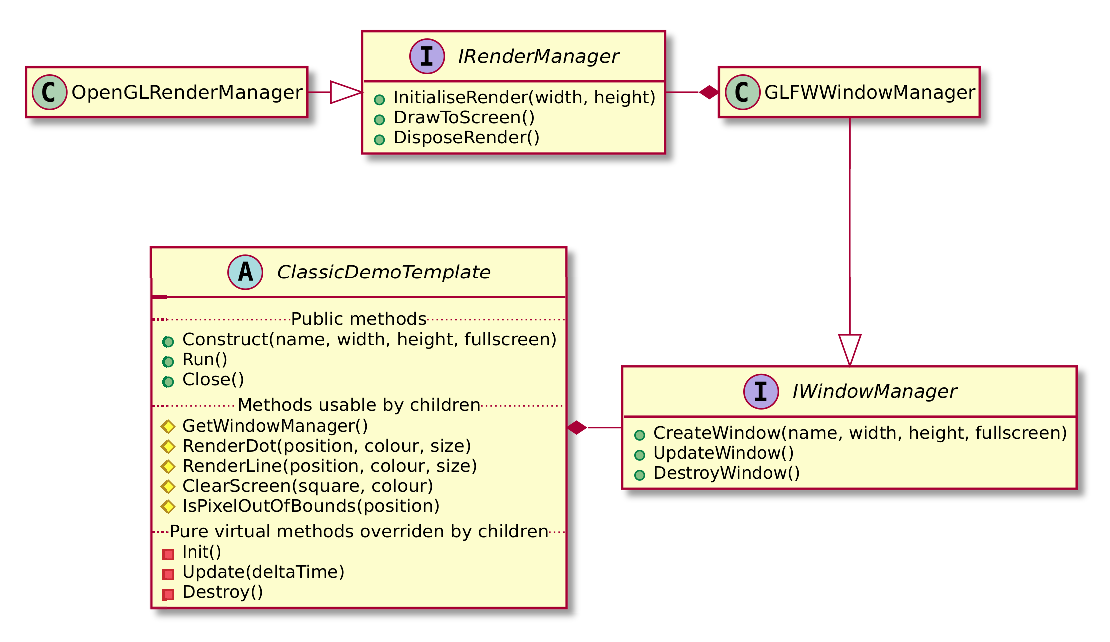
\includegraphics[width=15cm]{archivos/classicdemotemplateuml}
	\caption{Diagrama simplificado de la estructura del motor gráfico}
	\label{fig:classicdemotemplateuml}
\end{figure}

La figura [\ref{fig:classicdemotemplateuml}] presenta la estructura simplificada del motor gráfico.\\

Como se puede observar, el motor (\emph{ClassicDemoTemplate)} delega las tareas de gestión de la ventana en una interfaz cuyos métodos más relevantes permiten crear, actualizar y destruir la ventana. De este modo, el motor gráfico está completamente desacoplado de las tareas concretas de gestión de la ventana.\\

La implementación concreta de la interfaz (\emph{GLFWWindowManager}) utiliza, como su nombre indica, la librería GLFW para gestionar la ventana. Esta es una librería de código abierto y multiplataforma que hace más sencilla la gestión. No obstante, la implementación concreta está completamente desacoplada del sistema, por lo que si fuera necesario migrar a una tecnología distinta (como SDL, SFML o accediendo directamente a la API gráfica de Windows (WinAPI) o Linux (X11)), se podría hacer siempre y cuando esta nueva clase implementase la interfaz definida.\\

A su vez, \emph{GLFWWindowManager} hace uso de la interfaz \emph{IRenderManager}, que implementa \emph{OpenGLRenderManager}. Esto permite, una vez más, cambiar la tecnología de dibujado sin tener que cambiar necesariamente el sistema de ventanas. De este modo también se separa de forma efectiva todo el código relativo a la gestión de la ventana con respecto al código relativo al dibujado, lo que facilita la claridad y mantenimiento del código.\\

En nuestro caso, el dibujado se hace mediante OpenGL, una especificación para gráficos 3D multiplataforma. No obstante, OpenGL es utilizado como un mero mediador, cuyo único uso es el dibujado de una textura en pantalla. Es esta textura que se \emph{renderiza} de forma cíclica a la que el usuario tiene acceso y puede modificar, dibujando así en pantalla.\\

De este modo, la clase principal de nuestro motor \emph{(ClassicDemoTemplate)} no tiene responsabilidad directa sobre la gestión de la ventana y el dibujado, de modo que aunque las librerías o tecnologías utilizadas cambiasen, toda la lógica contenida en el motor seguiría siendo usable.\\

Como se puede observar en el diagrama, esta clase principal es una clase abstracta, lo que implica que debe ser implementada por una clase concreta para poder instanciarse. Toda demo que use este motor gráfico debe heredar de \emph{ClassicDemoTemplate}. Esto permite definir una estructura que todas nuestras demos deberán satisfacer para hacer un uso efectivo de nuestro motor.\\

En primer lugar, se exponen únicamente tres métodos, \emph{Construct}, \emph{Run} y \emph{Close}. Esto implica que cualquier demo ha de ser completamente usable mediante estos tres métodos.\\

A continuación, \emph{ClassicDemoTemplate} expone una serie de métodos que pueden ser utilizados únicamente por las demos, que heredan de esta clase. Estos métodos aportan funcionalidad común que resultan útiles en la mayor parte de las demos, como dibujar puntos y líneas o comprobar si un píxel determinado está dentro de los límites de la ventana.\\

Por último, hay tres métodos virtuales y privados que toda demo debe implementar: \emph{Init}, \emph{Update} y \emph{Destroy}. La llamada a estos método es gestionada por \emph{ClassicDemoTemplate}, por lo que el usuario tan sólo debe preocuparse de implementarlos. Los métodos \emph{Init} y \emph{Destroy} permiten inicializar y destruir las variables los datos propios de la demo. El método \emph{Update} es llamado en el bucle de ejecución del programa y recibe el tiempo sucedido desde el último fotograma. Este método contendrá toda la lógica necesaria para actualizar los datos que maneja nuestro programa a lo largo del tiempo. 

\subsection{La textura de dibujado y el píxel}

Para dibujar en pantalla en este proyecto, lo único que nos interesa es tener una zona de memoria en la que sepamos que podemos volcar datos. Es decir, no se usarán librerías externas para manipular los gráficos que se muestran en pantalla, si no que todas las transformaciones y el pintado en pantalla corre a nuestra cuenta.\\

Para ello, no obstante, el motor debe tener la capacidad de proveernos con un espacio de memoria en el que podamos pintar. Esto es responsabilidad de la implementación del \emph{IRenderManager.}\\

En nuestro caso, la clase \emph{OpenGLRenderManager} crea una textura basada en la altura, anchura y número de canales que queremos usar para la demo.\\

La altura y anchura se define en píxeles, y el número de canales se corresponde con la cantidad de canales de color que queremos. Por ejemplo, si quisiéramos un ventana monocromática, bastaría con definir un solo canal. Para crear una ventana que pueda representar (casi) cualquier color, necesitamos definir tres canales: rojo, verde y azul. Estos son los tres colores primarios de la luz. A través de combinaciones de los mismos podemos crear cualquier color. También podríamos definir incluso cuatro canales, tres para el color y un canal \emph{alfa} para la transparencia. Por defecto, se crea una textura asumiendo tres canales, cada uno de 8 bits, por lo que disponemos de 256 intensidades de color por canal y un total combinado de 16777216 colores posibles. La memoria reservada es pasada cada fotograma a OpenGL, como una textura. Es entonces estas librería la que se encarga de volcar estos datos en pantalla.\\

Sin embargo, desde el punto de vista del usuario, trabajar con la memoria directamente se hace, cuanto menos, incómodo. Para poder modificar cualquier píxel en pantalla es necesario tener en cuenta el número de canales, la posición y orden de cada color para un píxel determinado... y de pronto operar con píxeles, que debería ser algo sencillo, se convierte en una tarea compleja. Para poder sumar dos píxeles de pronto hay que sumar manualmente cada canal por separado, ¿pero qué pasa si la suma de dos canales supera el valor máximo que puede tener un color por canal, 255? La suma binaria de 128 más 128 resultaría en 0, con lo que si intentamos sumar dos rojos de intensidad media, obtendríamos como resultado el color negro (0), en lugar de un rojo intenso (255). Manejar esta textura se convierte de pronto en una tarea poco intuitiva, que nos llevará a cometer errores con mayor facilidad. Es por ello que se introduce el concepto del píxel a nivel del código.\\

%@startuml
%
%class Pixel
%{
%  + R
%  + G
%  + B
%  +Pixel()
%  +Pixel(value)
%  +Pixel(r, g, b)
%  +Pixel operator+(Pixel)
%  +Pixel operator-(Pixel)
%  +Pixel operator*(float)
%}
%
%hide empty members
%
%@enduml

\begin{figure}[h]
	\centering
	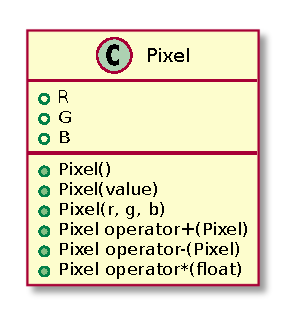
\includegraphics[width=6cm]{archivos/pixeluml}
	\caption{Estructura de un píxel en el motor gráfico}
	\label{fig:pixeluml}
\end{figure}

Un píxel [\ref{fig:pixeluml}] es una clase que contiene únicamente tres variables cuyo acceso es público. Estas variables son R(ed), G(reen) y B(lue), haciendo referencia al nombre del color (en inglés) asociado a cada canal. De este modo, la representación de un píxel coindide en memoria con la textura que hemos definido. De este modo, si bien a OpenGL le pasamos un conjunto de bytes, desde nuestro sistema los podemos organizar en píxeles.\\

Se proveen tres posibles constructores para un píxel. El constructor por defecto inicializa todos los valores a 0 (es equivalente a crear un píxel negro). También podemos proveer un solo valor al constructor, en cuyo caso se asignará este valor a cada canal (resultando en un color gris de mayor o menor intensidad) y por último podemos inicializar un píxel proveyendo un valor específico a cada canal. Es importante notar que por razones de eficiencia y simplicidad, no se hace ningún tipo de comprobación en la construcción, por lo que el intento de asignación de cualquier valor fuera de rango será equivalente al módulo de 256 de dicho valor. Por ejemplo, si intentamos asignar el valor 512 a un canal, será equivalente a asignarle un valor de 0.\\

Tras los tres métodos de construcción, se proveen tres operaciones matemáticas que se pueden realizar con píxeles, suma y resta de píxeles y multiplicación de un píxel por un escalar. La división de un píxel por un escalar no se provee ya que no resulta necesaria, en caso de que se quiera dividir el valor de un píxel, se multiplica por el inverso, consiguiendo el mismo resultado.\\

Por razones de consistencia, la suma y resta de píxeles tienen comprobaciones para evitar el desbordamiento. No sería deseable en nuestro sistema que la suma de dos píxeles cualesquiera, por ejemplo (128, 129, 130) y (200, 201, 202), resultara en un color oscuro. La suma de estos dos píxeles resultaría en (255, 255, 255), es decir, en blanco. Del mismo modo, la resta de dos pixeles siempre debería producir un color más oscuro, pero nunca más claro, por lo que cualquier resta de píxeles que pudiera producir desbordamiento (123 - 124 = -1, que equivale a 255, siendo este valor máxima intensidad) se resuelve en 0 (mínima intensidad o negro).\\

La multiplicación de un píxel por un escalar no se comprueba, ya que dado su uso en el sistema, no resulta práctico. El usuario ha de ser consciente, sin embargo, que sólo las operaciones en que el valor del escalar está entre 0 y 1 son seguras, ya que la multiplicación de un píxel por cualquier valor inferior a 0 o superior a 1 puede producir, potencialmente, desbordamiento (64 * 2 = 128, no desborda, comportamiento esperado; 128 * 2 = 256, resulta en 0, comportamiento inesperado).\\

El motivo por el que la suma y la resta son operaciones comprobadas mientras que la construcción y la multiplicación no lo son está justificado. Los valores de construcción y multiplicación en nuestro sistema están siempre controlados, y en la mayor parte de los casos predefinidos, por lo que se asegura de antemano que no se va a producir un desbordamiento, y por tanto poner comprobaciones para estas operaciones tan sólo supondría en la pérdida de eficiencia (ahora bien, es necesario hacer un uso consciente de las mismas). La suma y la resta necesitan comprobaciones ya que la mayor parte de sumas y restas que se producen son sobre valores generados dinámicamente, sobre los que no tenemos control directo, por lo que no podemos asegurar que no se va a producir desbordamiento, y debemos, por tanto, prevenirlo.\\

Del mismo modo, se provee acceso directo al valor de cada píxel, no solo para su lectura, si no también para su escritura. Esto se hace por conveniencia, pues en ocasiones puede que solo queramos modificar un canal concreto. Debe tenerse en cuenta, no obstante, que estas operaciones pueden provocar desbordamiento. La razón de esta decisión es nuevamente el hecho de que cuando se accede de forma directa al valor de un canal, se hace de forma controlada, por lo que se programa en torno a la posibilidad de desbordamiento.\\

Este sistema busca ser eficiente, por lo que sólo se realizan comprobaciones cuando se consideran estrictamente necesarias. Esto fuerza, no obstante, a hacer un uso consciente del sistema.

\subsection{Detectar input}

Por básica que pueda parecer la detección de entradas de teclado, esta característica no fue implementada hasta un estado relativamente avanzado del desarrollo del proyecto. Aunque esto pueda resultar difícil de entender desde el punto de vista del usuario, desde el punto de vista del desarrollador, las entradas de teclado sirven principalmente para "jugar" con la demo y para ajustar valores, es decir, que resultan útiles en el proceso de refinamiento de la demo, pero son irrelevantes en el proceso de creación de la misma. Es por ello que disponer de \emph{input} para las demos no es algo que se priorizara, ya que estaba mucho más interesado en el desarrollo de los algoritmos y métodos necesarios para cada demo que no en poder "jugar" con los resultados.\\

No obstante, llegó un punto en el desarrollo en el que las demos, además de ser funcionales, debían ser manipulables, modificables de forma dinámica, y fue en este momento cuándo se planteó la pregunta de cómo gestionar las entradas de teclado.\\

Las entradas de teclado se gestionan desde la ventana, por lo que tenía claro que su gestión debería ser parte de la responsabilidad de \emph{GLFWWindowManager}. Era importante, sin embargo, saber en qué eventos de teclado estaba interesado.\\

Estos eran los eventos que me interesaban: saber el momento en que la tecla se pulsa por primera vez, saber el momento en el que la tecla se suelta y saber si la tecla se está manteniendo pulsada o no. Sin embargo, GLFW sólo daba acceso directo a saber si la tecla estaba pulsada o no, por lo que la lógica para el resto de eventos debía ser implementada por mi parte.\\

GLFW permitía otra opción, además, en lugar de preguntar por el estado de una tecla concreta, es posible pasarle un método delegado que sea llamado cada vez que se produce un evento, de forma que este método sobre el que nosotros tenemos control pueda gestionar los eventos en los que estamos interesados. Por razones de simplicidad y mantenibilidad, decidí optar sin embargo por la opción de preguntar por el estado de las teclas.\\

Esta opción sin embargo planteaba un problema de eficiencia: la única forma de saber si una tecla cualquiera está pulsada o no es almacenando y actualizando el estado de todas las teclas. Esto implicaría tener que estar actualizando el estado de más de 100 teclas cuando tan sólo tenemos interés en unas pocas. Y precisamente lo que decidí fue añadir un método que permitiera registrar interés en una tecla. Esto hace que la gestión de \emph{input} en una demo sea ligeramente más compleja (para poder preguntar por el estado de una tecla, esta debe haberse registrado previamente). Sin embargo, a cambio de esta ligera complejidad añadida, hay una gran ganancia en rendimiento, ya que en lugar de actualizar el estado de \emph{todas} las teclas del teclado por fotograma, sólo actualizaremos el estado de aquellas que nos interesan, y en caso de no tener interés en ninguna, simplemente no se tendrán en cuenta las entradas de teclado, no impactando en ningún modo al rendimiento del programa.\\

%@startuml
%
%interface IWindowManager {
%  +RegisterKeyInput(key)
%  +IsKeyPressed(key)
%  +IsKeyHeld(key)
%  +IsKeyReleased(key)
%  +IsKeyUp(key)
%}
%
%class KeyState << (S,#FF7700) Struct >>
%{
%  +IsPressed
%  +IsHeld
%  +IsReleased
%  +IsUp
%}
%
%hide empty members
%
%@enduml

\begin{figure}[h]
	\centering
	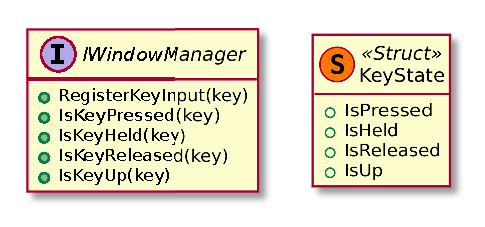
\includegraphics[width=10cm]{archivos/inputuml}
	\caption{Funciones y estructuras del sistema de input}
	\label{fig:input}
\end{figure}

\subsection{Dibujar texto}

Al igual que con el input, la necesidad de dibujar texto no se hizo aparente hasta un estado más avanzado de desarrollo del proyecto. Una vez en la tesitura en la que poder dibujar texto en pantalla era necesario, fue necesario dedicar un tiempo de análisis.\\

Inicialmente pensé en usar una librería y estuve investigando cuál podía satisfacer mejor mis objetivos. glfreetype\footnote{\url{https://github.com/benhj/glfreetype}} parecía bastante adecuada, tratándose de una librería pequeña, concisa y aparentemente sencilla de utilizar.\\

A mitad camino del proceso de integración de esta librería, no obstante, me empecé a plantear hasta qué punto tenía sentido utilizar una librería externa para el dibujado de texto en pantalla. Al fin y al cabo, uno de mis objetivos con este trabajo era que todo aquello que estuviera dibujado en pantalla hubiera sido desarrollado de forma exclusiva por mi, sin usar librerías externas. Las únicas librerías que usa este trabajo (GLFW y OpenGL) son utilizadas con el único objetivo de facilitar la implementación y no salirse del ámbito de este estudio. No obstante, este no parecía ser el caso para el dibujado de texto en pantalla.\\

No obstante, implementar un sistema de dibujado de texto parecía complejo, \emph{a priori}. Es por ello que me plantée, ¿cuál es la forma más sencilla y rápida en la que podría dibujar texto en pantalla?

Tras un tiempo de análisis, llegué a la conclusión de que implementar un sistema de dibujado de texto era una tarea sencilla y que se podía considerar dentro del ámbito de este proyecto. Por tanto, no sería necesario usar librerías externas. Este sistema de texto debería ser lo más sencillo posible, no obstante, y tendría ciertas limitaciones.\\

La mayoría de librerías de texto son capaces de leer formatos de fuente como TrueType o OpenType, además, para cada letra dibujan un \emph{quad} mediante OpenGL al que aplican una textura con transparencia representando la letra. Este proceso es más complejo de lo asumible para este proyecto, pero por suerte, no era necesario seguirlo.\\

Mi sistema estaría basado en las siguientes ideas: 
\begin{itemize}
	\item Es necesario un método para dibujar caracteres individuales
	\item Es necesario un método para dibujar cadenas de caracteres
	\item Todo lo que necesita un carácter para ser dibujado es posición, color y tamaño.
	\item La forma más sencilla de usar una fuente es crear nuestra propia fuente, que vaya embebida en el código
	\item Cualquier carácter puede ser definido dentro de una cuadrícula de 5x5 unidades como en [\ref{cod:fontA}]
	\item No es necesario diferenciar entre mayúscula y minúscula (tener doble representación para las letras supone una pérdida de espacio y tiempo)
\end{itemize}

\begin{lstlisting}[style=C-color, caption={Método que renderiza un sólo caracter},label=cod:fontA]
const char *Characters::A{
    "_###_"
    "#___#"
    "#####"
    "#___#"
    "#___#"
};
\end{lstlisting}

Así pues, la tareas que realmente más tiempo llevan en un sistema como el definido es crear todos los caracteres que se necesitan, que en mi caso son todas las letras del alfabeto inglés, los números y algunos caracteres especiales. Una vez hecho esto, se inserta todos estos caracteres dentro de un mapa estático cuya clave sea un caracter y el valor sea la cuadrícula 5x5 que lo representa.\\

\begin{lstlisting}[style=C-color, caption={Método que renderiza un sólo caracter},label=cod:rendercharacter]
void ClassicDemoTemplate::RenderCharacter(char character, int x, int y, int scale, const Pixel &colour)
{
    if (character < 0 || character == ' ')
    {
        return;
    }

    const char *c = Characters::GetCharactersMap()[character];

    for (int i = x; i < x + 5 * scale; i++)
    {
        for (int j = y; j < y + 5 * scale; j++)
        {
            int offsetX = (i - x) / scale;
            int offsetY = (j - y) / scale;

            if (c[offsetY * 5 + offsetX] != ' ')
            {
                screen[j * width + i] = colour;
            }
        }
    }
}
\end{lstlisting}

Una vez tenemos el mapa de caracteres, dibujar un caracter en pantalla es de lo más sencillo [\ref{cod:rendercharacter}]. Tras una comprobación inicial para saber si el carácter no es válido o es un espacio (que obviamente no se dibuja), lo primero que hacemos es obtener la cuadrícula 5x5 que se asocia con el caracter a dibujar.\\

Una vez hecho esto, recorremos la cuadrícula en vertical y horizontal. La cantidad de píxeles que recorremos en cada dirección es equivalente al tamaño de la cuadrícula (5) multiplicado por la escala del caracter. Así pues, un carácter con escala 1 tendrá un grosor de línea de un píxel y ocupara un espacio de 5x5 píxeles mientras que un caracter con escala 2 tendrá 2 píxeles de grosor de línea y ocupará un espacio de 10x10 píxeles.\\

Tras esto hacemos una conversión sencilla para hallar, dadas unas coordenadas cualesquiera dentro del bucle, las coordenadas de la cuadrícula que le corresponden. Una vez halladas, se comprueba la posición de la cuadrícula. Si es un espacio en blanco (en el ejemplo [\ref{cod:fontA}] se sustituyen los espacios por barras bajas por cuestión de claridad visual) no se rellena, mientras que si esa posición de la cuadrícula no es un espacio, se pinta el píxel con el color correspondiente.\\

\begin{lstlisting}[style=C-color, caption={Método que renderiza una cadena de caracteres},label=cod:rendertext]
void ClassicDemoTemplate::RenderText(const char *text, int posX, int posY, int scale, const Pixel &colour)
{
    std::string txt(text);
    for (auto &c : txt)
    {
        c = toupper(c);
    }

    for (auto c : txt)
    {
        RenderCharacter(c, posX, posY, scale, colour);
        posX += 6 * scale;
    }
}
\end{lstlisting}

El método para dibujar texto es también muy sencillo, como se puede ver en el ejemplo [\ref{cod:rendertext}]. Lo primero que hacemos es poner todos los caracteres en mayúscula, pues como ya habíamos decidido antes, es más práctico tener un único conjunto de letras. A continuación, por cada caracter que forma el texto invocamos a la función de dibujado de caracter [\ref{cod:rendercharacter}]. Por cada dibujado, aumentamos la posición horizontal, de modo que el próximo caracter se dibuje a 6 unidades de distancia del inicio del caracter anterior (es decir, se deja una unidad de 1 espacio entre uno y otro carácter, ya que un caracter ocupa 5 unidades).

\subsection{Dibujar puntos}

La necesidad de dibujar puntos en el motor gráfico no llegó hasta un punto algo más avanzado del desarrollo. Al fin y al cabo, dibujar un punto de una unidad de tamaño en pantalla equivale a dibujar un píxel, y para dibujar un píxel, basta con acceder a nuestra textura y modificar los valores deseados.\\

Argumentablemente se podría decir que mediante un control en el dibujado de puntos podemos asegurar que nuestro programa nunca pinte fuera de pantalla, pudiendo provocar errores, pero nuevamente, si podemos asegurar un entorno controlado en el que sabemos que ningún píxel estará fuera de pantalla, hacer esta comprobación es redundante, una pérdida de rendimiento para nada.\\

Sin embargo, todo esto cambia cuando consideramos que un punto no es necesariamente un píxel. Un punto de dos unidades ocupará 2x2=4 píxeles, y un punto de tres unidades ocupará 3x3=9 píxeles, si bien a nivel conceptual sigue siendo un punto. Y en este momento se presenta otra pregunta, ¿qué pasa si un punto de por ejemplo 4 unidades tiene solo medio "cuerpo" en pantalla? Lo lógico sería que se viera la parte del mismo que está en pantalla. Sin embargo, si no controlamos los límites de dibujado, esto puede llevar a comportamientos inesperados (al intentar volcar datos fuera de la memoria de la textura, pudiendo reescribir datos cualesquiera).\\

\begin{lstlisting}[style=C-color, caption={Método para dibujar puntos},label=cod:renderdot,escapechar=|]
void ClassicDemoTemplate::RenderDot(int x, int y, const Pixel &colour, int dotSize)
{
    for (int i = 0; i < dotSize; i++)
    {
        for (int j = 0; j < dotSize; j++)
        {
            int offsetX = x + i;
            int offsetY = y + j;

            if (IsPixelOutOfBounds(offsetX, offsetY))
            {
                continue;
            }

            screen[offsetY * width + offsetX] = colour;|\label{line:directpaint}|
        }
    }
}
\end{lstlisting}

Es en este momento cuando se crea un método que permita el dibujado de puntos en pantalla [\ref{cod:renderdot}] de forma controlada y segura. Este método permite dibujar puntos de cualquier tamaño con la garantía de que sólo se accederá a memoria dentro de pantalla.\\

Pero el uso de este método es nuevamente un compromiso. A cambio de tener la posibilidad de tener puntos con escala y que no se dibujan fuera de pantalla, se compromete la eficiencia, pues una operación de una sola línea [\ref{line:directpaint}] pasa a convertirse en un método de complejidad cuadrática y con comprobaciones que interrumpen un flujo de ejecución lineal. Es por ello que esta funcionalidad sólo debe usarse cuando tenga sentido, es útil si queremos pintar unos pocos puntos de tamaño variable o que pueden estar dentro o fuera de la pantalla, pero no tendría sentido utilizar este método si se requiere repintar toda la pantalla píxel a píxel.

\subsection{Dibujar rectángulos}

El dibujado de rectángulos en pantalla es una funcionalidad especialmente útil para el borrado de pantalla o de ciertas áreas de la misma.\\

\begin{lstlisting}[style=C-color, caption={Métodos de repintado en pantalla},label=cod:clearscreen]
void ClearScreen(const Pixel &colour);

void ClearScreen(int x1, int y1, int x2, int y2, const Pixel &colour);
\end{lstlisting}

\emph{ClassicDemoTemplate} provee dos funciones de dibujado diferentes [\ref{cod:clearscreen}], rellenar toda la pantalla dado un color o rellenado de una subsección de la pantalla.\\

Para rellenar una subsección de la pantalla, es necesario aportar, además de un color, las coordenadas de dos puntos que representen la esquina superior izquierda del rectángulo y la esquina inferior derecha. Este método comprueba la validez de la coordenadas pasadas y si alguna de las coordenadas está fuera de pantalla, pinta la sección correspondiente, pero sin sobrepasar los límites. El uso de esta segunda función se recomienda siempre que se pueda frente al redibujado completo de toda la pantalla, pues si bien recorrer todos los píxeles en pantalla es una operación sencilla, es costosa a nivel temporal.

\subsection{Dibujar líneas}

El dibujado de líneas no fue necesario hasta un estado avanzado del desarrollo, cuando para poder representar modelos geométricos era como mínimo necesario poder dibujar sus aristas mediante líneas.\\

El código para dibujar líneas lo reutilicé de un proyecto anterior que yo mismo había desarrollado\footnote{\url{https://github.com/donluispanis/PaintLike}}. Este código, a su vez, estaba inspirado en el algoritmo de pintado de líneas de Bresenham\footnote{\url{https://en.wikipedia.org/wiki/Bresenham\%27s_line_algorithm}}, si bien era ligeramente distinto en su implementación. 

\begin{figure}[h]
	\centering
	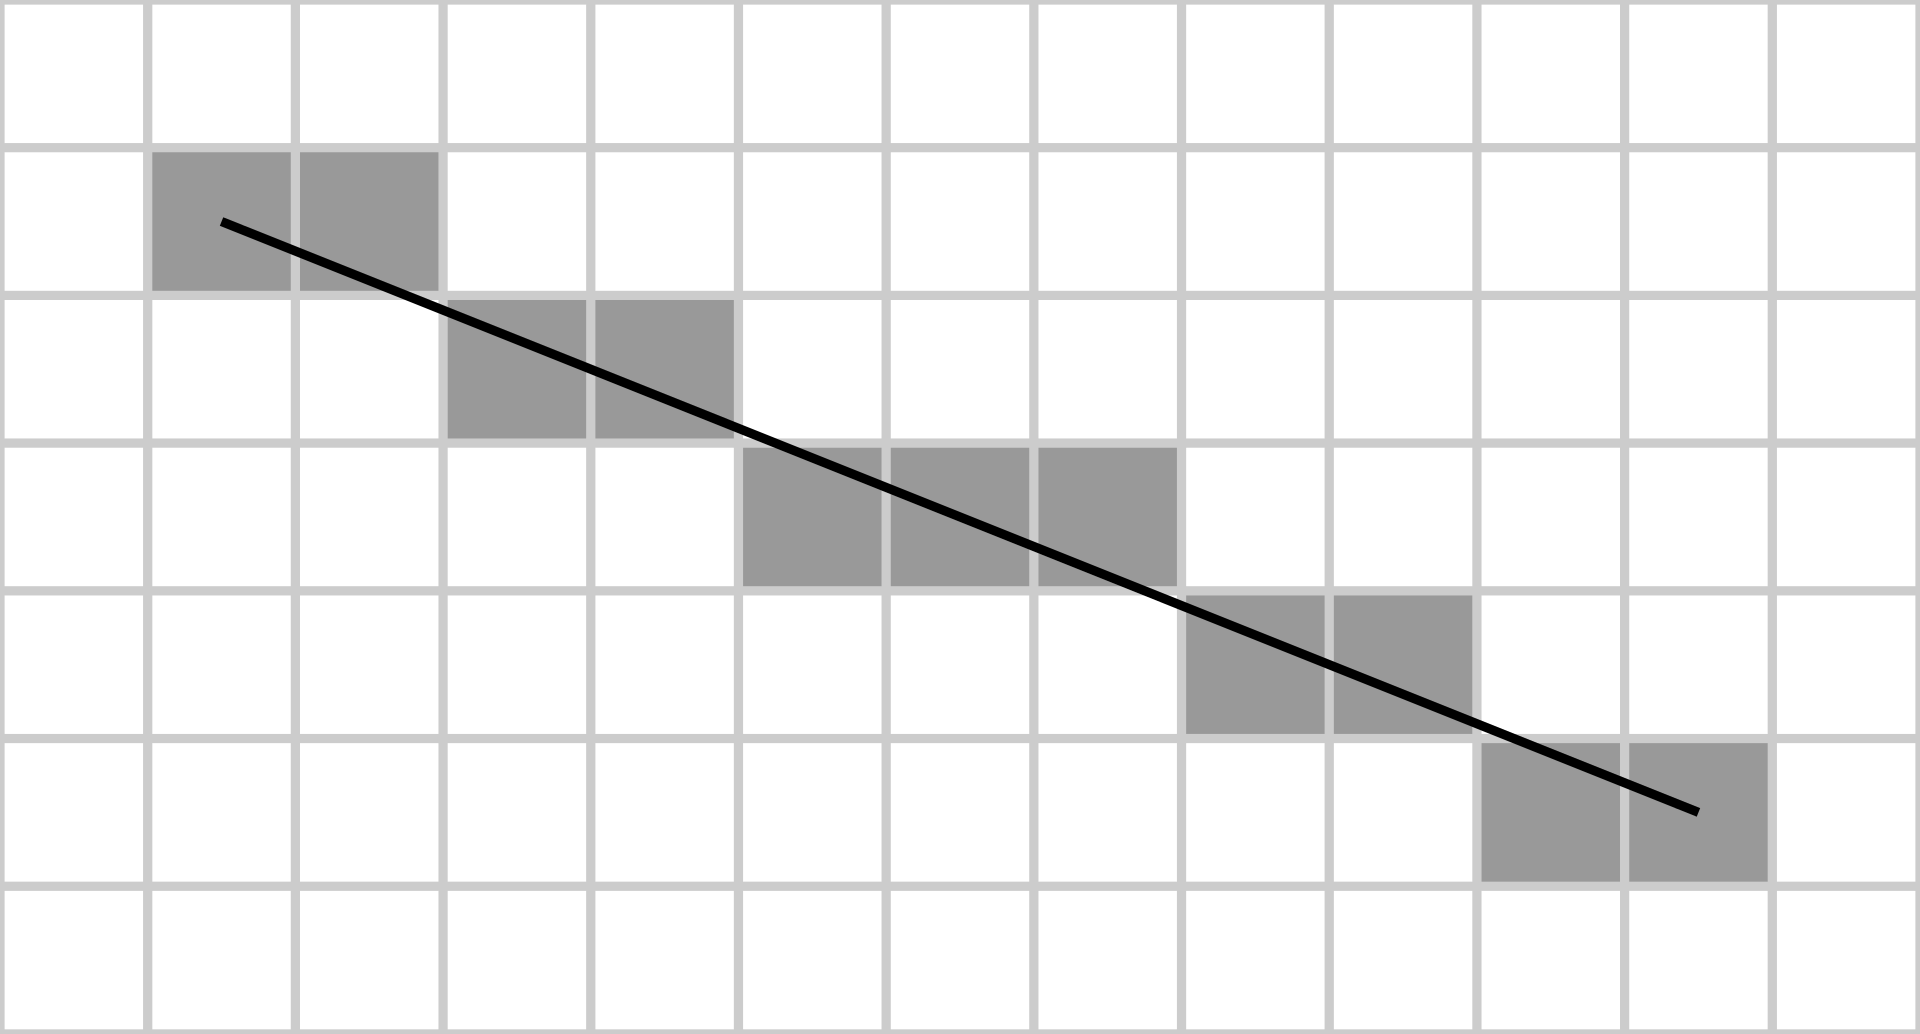
\includegraphics[width=8cm]{archivos/bresenham}
	\caption{Pintado de líneas en pantalla (adaptación de una línea a una cuadrícula) - Fuente: \href{https://en.wikipedia.org/wiki/Bresenham\%27s_line_algorithm\#/media/File:Bresenham.svg}{Wikipedia}}
	\label{fig:bresenham}
\end{figure}

En esencia, esta es la lógica que sigue el código de pintado:

\begin{itemize}
	\item Dados el punto de inicio y el punto de fin de la recta, calcular la pendiente de la recta a partir de los mismos.
	\item Si la pendiente es inferior a 45º, iterar desde el punto de inicio de la recta hasta el punto final, incrementando siempre la posición horizontal e incrementando sólo la posición vertical cuando el error acumulado es mayor que uno.
	\item Si la pendiente es superior a 45º, iterar desde el punto de inicio de la recta hasta el punto final, incrementando siempre la posición vertical e incrementando sólo la posición horizontal cuando el error acumulado es mayor que uno.
\end{itemize}

\begin{lstlisting}[style=C-color, caption={Versión simplificada y reducida del código para dibujar líneas en pantalla},label=cod:drawline]
void RenderLine(int x1, int y1, int x2, int y2, const Pixel &colour)
{
    float slope = GetSlope(x1, y1, x2, y2);

    //Slope < 45º
    if (slope <= 1.f)
    {
        DrawLineWithSmallSlope(x1, y1, x2, y2, colour, slope);
    }
    //Slope > 45º
    else
    {
        DrawLineWithBigSlope(x1, y1, x2, y2, colour, slope);
    }
}

void DrawLineWithSmallSlope(int x1, int y1, int x2, int y2, const Pixel &colour, float slope)
{
    float acummulatedError = 0.f;  
    int auxX = x1, auxY = y1; //auxiliar point that we will increment from the old point to the new one

    int signX, signY;
    GetSigns(x1, y1, x2, y2, signX, signY);

    //While we don't reach the desired pixel position
    while (auxX != x2 || auxY != y2)
    {

        RenderDot(auxX, auxY, colour);
        
        auxX += signX; //Increment X until it reaches the target

        acummulatedError += Fast::Abs(slope); //When this reaches 1, we increment Y

        if (acummulatedError >= 1.f)
        {
            auxY += signY;
            acummulatedError -= 1.f;
        }
    }
}
\end{lstlisting}

El código que se muestra en [\ref{cod:drawline}] es tan solo una versión simplificada, reducida y no funcional de la implementación en código del algoritmo para el dibujado de rectas en pantalla, pero que pretende ser suficiente para ejemplificar cómo se traduce la lógica anteriormente descrita al código.\\

Como se ha comentado previamente, este código se inspira en el algoritmo de Bresenham, pero no lo sigue. Una de las mayores diferencias es que el algoritmo de Bresenham sólo utilizaba números enteros, pues cuando fue desarrollado, las operaciones con números en coma flotante eran lentas y se realizaban por \emph{software}. Hoy en día, no obstante, se realizan por \emph{hardware}, y no suponen en muchos casos un coste significativo con respecto a las operaciones con enteros.\\

Además, según las necesidades han ido variando, se ha ido añadiendo funcionalidad adicional al pintado de líneas:

\begin{itemize}
	\item Posibilidad de definir un grosor de línea
	\item Posibilidad de definir un color de inicio y de final, sobre los que se interpola (dando una sensación de degradado)
\end{itemize}
\chapter{Demos clásicas}

\section{Fuego}

\subsection{Investigación inicial}

Una demo que simule un efecto de fuego se podría considerar algo así como el "hola mundo" de la demoscene. Es un ejercicio sencillo con un resultado final bastante espectacular.\\

Tras una búsqueda de información inicial, pude encontrar también dos sitios diferentes en los que se explicaba cómo crear un efecto de fuego.\\ 

En el canal de YouTube de Creature Mann\footnote{\url{https://www.youtube.com/user/kjlg74/featured}} se explica la base teórica para crear un efecto de fuego sencillo\footnote{\url{https://www.youtube.com/watch?v=_SzpMBOp1mE}}. A este vídeo le siguen un par de vídeos de este mismo creador\footnote{\url{https://www.youtube.com/watch?v=iezD8B1ym3w}}\footnote{\url{https://www.youtube.com/watch?v=206TEPBOnLc}} en los que itera sobre el efecto anteriormente creado, añadiendo complejidad (como la posibilidad de controlar la dirección del fuego o trazar un camino que se prende fuego). Por desgracia, los enlaces provistos al código que estos vídeos muestran están caídos, por lo que el código no es accesible. No obstante, la parte argumentablemente más importante, la explicación teórica del efecto, se hace en el primer vídeo.\\

Otra página que ofrece una descripción muy buena del efecto es Lode's Computer Graphics Tutorial\footnote{\url{https://lodev.org/cgtutor/fire.html}}. Esta página sí que aporta código, aunque decidí ignorar la implementación (para evitar que condicionara mi propio desarrollo) y centrarme únicamente en la explicación teórica que se ofrecía, muy similar a la del vídeo anterior aunque más técnica.\\

\subsection{Planteamiento formal}

El fuego es un efecto muy sencillo tanto a nivel teórico como de implementación. Consiste en la convolución de una matriz como la de la figura [\ref{fig:firematrix}] a lo largo de una matriz que tan sólo contiene valores en su fila inferior. Al aplicar esta operación de abajo a arriba, se obtiene un conjunto de valores [\ref{fig:fire_whitegrid}] que al ser asociados a un set concreto de colores [\ref{fig:fire_colouredgrid}], dan una sensación similar al fuego.\\

\begin{figure}
	\begin{equation}
		\begin{bmatrix}
			0 & 0 & 0 \\
			0 & 0 & 0 \\
			\frac{1}{3} & \frac{1}{3} & \frac{1}{3}
		\end{bmatrix}
	\end{equation}
	\caption{Matriz de convolución para generar efecto de fuego}
	\label{fig:firematrix}
\end{figure}

Otra forma de entender esta operación es la siguiente: el valor de cada píxel se deduce de la media del valor de los tres píxeles adyacentes por debajo de él. Para que este efecto se produzca de forma efectiva, la fila inferior de píxeles se suele rellenar con valores aleatorios. De esta forma, la tendencia natural de este modelo es la de disiparse.\\

El único caso en el que no se produciría disipación sería en el que todos los valores de la fila inferior se inicializaran al máximo (en cuyo caso todos los píxeles acabarían con el mismo valor). Para cualquier otra situación, se produce una atenuación progresiva de los valores. 

\begin{figure}[h]
	\centering
	\begin{subfigure}[b]{0.45\textwidth}
		\centering
		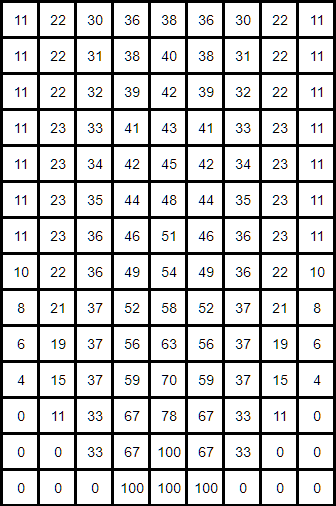
\includegraphics[width=5.09cm]{archivos/fire_whitegrid}
		\caption{Valores resultantes tras convolucionar iterativamente la matriz [\ref{fig:firematrix}] por una matriz de ceros, con valores solo en la fila inferior}
		\label{fig:fire_whitegrid}
	\end{subfigure}
	\begin{subfigure}[b]{0.45\textwidth}
		\centering
		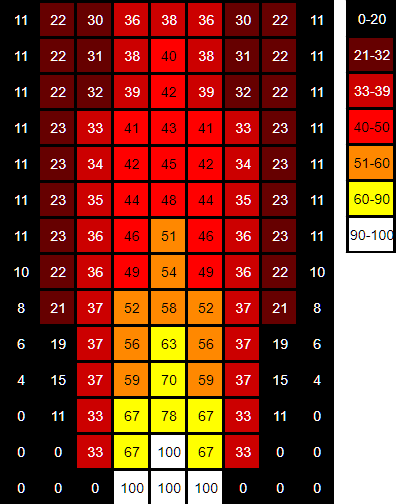
\includegraphics[width=6cm]{archivos/fire_colouredgrid}
		\caption{Efecto resultante de asociar determinados rangos de valores a un set de colores preestablecido}
		\label{fig:fire_colouredgrid}
	\end{subfigure}
\end{figure}

Dado el comportamiento descrito, será necesario realizar los siguientes pasos:
\begin{itemize}
	\item Implementar una forma de realizar degradados (o mapas de color)
	\item Reservar e inicializar una matriz a cero, con valores aleatorios en su fila inferior
	\item Implementar el comportamiento de convolución de la matriz [\ref{fig:firematrix}]
\end{itemize}

\subsection{Implementación}

Para poder crear degradados, se crea la función \emph{GenerateGradient} que dado un conjunto de \emph{ColourStamp} y un tamaño, interpola los valores de colores pasados para generar un degradado continuo en \emph{colourMap}.\\

\begin{lstlisting}[style=C-color, caption={Método para crear gradientes de color},label=cod:generateGradient]
static void GenerateGradient(std::vector<ColourStamp> colours, Pixel* colourMap, int colourMapSize);
\end{lstlisting}

\emph{ColourStamp} (marca de color) es una estructura formada por dos variables: un color y un número decimal (que puede oscilar entre 0 y 1). Este número señala la posición de este color en el gradiente o mapa de color, siendo 0 el inicio y 1 el final. 

\begin{figure}[h]
	\centering
	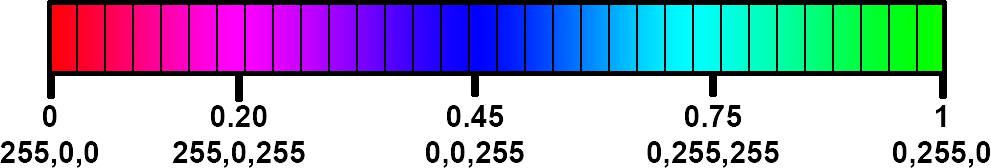
\includegraphics[width=12cm]{archivos/colourGradient}
	\caption{Degradado en 32 celdas dadas 5 marcas de color}
	\label{fig:colourGradient}
\end{figure}

De este modo, si llamamos a la función \emph{GenerateGradient} con los valores para las marcas de color representados en la figura [\ref{fig:colourGradient}] y pasamos un \emph{array} con capacidad para 32 valores, este método producirá un set de colores similar al ilustrado. Esto se hace mediante una interpolación lineal entre los valores que se pasan, creando un degradado de forma progresiva.\\

Una vez tenemos implementado este método, ya podemos crear un degradado de colores de forma sencilla y cómoda, automatizando el proceso de crear un mapa de color para el fuego.\\

Para nuestra implementación, en lugar de asignar a un rango de valores un color específico, asignaremos un color por valor entero. Esto permitirá un resultado más realista, al disponer de una mayor cantidad de colores. Cada celda de nuestra matriz de valores estará formada por un byte. Esto implica que cada celda podrá tener 256 valores distintos, y que por tanto necesitaremos generar un degradado que nos devuelva 256 colores.\\

Creamos un mapa de valores de un byte de tamaño, lo inicializamos a 0 e inicializamos aleatoriamente algunas de las celdas de la fila inferior a su valor máximo (255).\\

\begin{lstlisting}[style=C-color, caption={Creación e incialización del mapa de valores},label=cod:screenMapping,escapechar=|]
screenMapping = new unsigned char[width * height];

for (int i = width * (height - 1), n = width * height; i < n; i++)
{
    if (Fast::Rand() % 10 == 0)|\label{line:fastRand}|
    {
        screenMapping[i] = 255;
    }
}
\end{lstlisting}

Como podemos ver en la línea [\ref{line:fastRand}], hacemos uso de una función propia para la generación de números aleatorios. Esta función está basada en el algoritmo \emph{Xorshift}\footnote{\url{https://en.wikipedia.org/wiki/Xorshift}} de George Marsaglia. La apromaximación usada está basada en una respuesta de \emph{StackOverflow}\footnote{\url{https://stackoverflow.com/questions/1640258/need-a-fast-random-generator-for-c}}.\\

La decisión de usar nuestro propio generador de números aleatorios se debe a que el usualmente provisto por la STL \footnote{\url{https://en.wikipedia.org/wiki/Standard_Template_Library}} es innecesariamente lento y complejo para nuestras necesidades. Para nuestro caso, no necesitamos un algoritmo que pase todos los tests de aleatoriedad\footnote{\url{https://es.wikipedia.org/wiki/Pruebas_de_aleatoriedad}}, con tal de que sea suficientemente "aleatorio al ojo" y sea rápido, nos basta.\\

Una vez hecho esto, tan sólo queda implementar el algoritmo principal, que cree el efecto de fuego sobre el mapa de valores previamente creado, de acorde a la operación descrita en la figura [\ref{fig:firematrix}] y asocie dichos valores con un color generado por la función \emph{GenerateGradient} [\ref{cod:generateGradient}].\\

\begin{lstlisting}[style=C-color, caption={Algoritmo básico de efecto de fuego},label=cod:simpleFire,escapechar=|]
for (int i = width * (height - 1); i >= 0; i--)
{
    int lowerCell = width + i;|\label{line:simpleFire1}|
    int newCellValue = screenMapping[i] = (screenMapping[lowerCell + 1] + screenMapping[lowerCell] + screenMapping[lowerCell - 1]) / 3.0;|\label{line:simpleFire2}|
    pixels[i] = colourMap[newCellValue];|\label{line:simpleFire3}|
}
\end{lstlisting}

En el código [\ref{cod:simpleFire}] podemos  ver el algoritmo de generación de fuego en su forma más simple. Recorremos la pantalla de abajo a arriba y operamos por cada píxel. En la línea [\ref{line:simpleFire1}] obtenemos, para una posición dada en el mapa de valores, la posición del valor inmediatamente por debajo del mismo. Una vez obtenida esta posición, operamos haciendo la media usando su valor y los adyacentes. Guardamos el resultado como nuevo valor y usamos a la vez este nuevo valor para asociar un nuevo color al píxel en pantalla (línea [\ref{line:simpleFire3}]). Los valores más altos (255) representan tonos blancos y/o amarillentos, mientras que los valores intermedios representarán valores rojizos y los valores más bajos tendrán asociados colores más oscuros.\\

El resultado de aplicar este algoritmo resulta en una imagen estática y de aspecto poco realista [\ref{fig:fire_simple}], pero que ya se empieza a parecer al efecto que buscamos.\\

\begin{figure}[h]
	\centering
	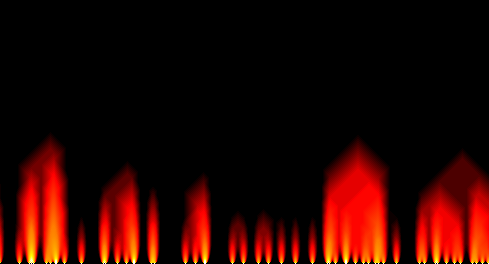
\includegraphics[width=8cm]{archivos/fire_simple}
	\caption{Fuego estático, usando el algoritmo en [\ref{cod:simpleFire}]}
	\label{fig:fire_simple}
\end{figure}

\subsection{Refinamiento}

Una vez tenemos el efecto de fuego a nivel básico, es el momento de iterar sobre la idea y ver cómo mejorarla. A continuación se listan y explican las medidas tomadas, mostradas en el orden en que se aplicaron:

\begin{itemize}
	\item \textbf{Hacer fuego dinámico}: una vez obtenido un fuego estático, era el momento de darle movimiento, y que tuviera un efecto realista. Inicialmente probé con una técnica que se sugería en algunos de los tutoriales que había seguido: en lugar de dibujar el fuego de abajo a arriba, dibujarlo de arriba a abajo y aleatorizar la base, de forma que las variaciones en el fuego derivaran a partir de las variaciones en la base.
	
	El resultado no me dejó convencido. Cuando uno observa un fuego o una llama, la parte más cambiante del fuego no es la base, la base es siempre estable y es la parte superior la que más titila / oscila. Por tanto no tenía para mí sentido generar dinamismo aleatorizando la base.
	
	Una llama se caracteriza a menudo por tener una intensidad variante, y fue esto lo que me decidí por implementar: la base permanecería estable, la llama tendría un factor de aleatoriedad.
	
	Tras un ensayo de prueba y error ajustando valores, y teniendo que retocar la posición y tono de los colores en el gradiente, se llegó al siguiente código \lstinline{(Fast::Rand() % 4 == 0 ? 2 : 0)} que se puede ver aplicado en [\ref{cod:finalFire}]. Básicamente este código altera levemente el valor de intensidad del píxel de forma aleatoria, con un 25\% de posibilidades de que el valor del píxel se vea incrementado. 
	
	El resultado puede verse en [\ref{fig:fire_final}]. La base sobre la que se aplica es la misma que en la figura [\ref{fig:fire_simple}], sin embargo, el resultado resulta más convincente / natural gracias a que se introduce una pequeña aleatoriedad en la intensidad del píxel, introduciendo cierta dispersión.
	
	\item \textbf{Más colores}: una vez tenía el fuego básico creado llegó el momento de ponerse creativo y añadir más degradados, que pudieran ser aplicados para crear fuegos de distintos colores. Al degradado de fuego básico (blanco - amarillo - rojo - negro) se le añadieron dos nuevos degradados, un fuego estilo neón (rosa - verde - azul - negro) y un degradado en blanco y negro (blanco - gris - negro).
	
	Además, el código para generar degradados, que inicialmente estaba en el mismo archivo que el fuego, se separó a su propio archivo y clase. Por último, y en vistas de que el código para crear un degradado ocupaba mucho espacio (debido a la necesidad de definir las marcas de color) y que potencialmente sería reutilizado por otros efectos que usasen degradados, el código se movió a una clase común con inicialización estática. De este modo, desde el inicio de la ejecución están disponibles los vectores de marcas de color necesarios para generar distintos patrones (fuego, neón, blanco y negro, arcoiris...) mediante la función \emph{GenerateGradient}.
	
	\item \textbf{Manipulación del fuego}: una vez teníamos distintos colores, era necesario poder cambiar entre ellos. Fue en este momento cuando se incorporó al motor la capacidad de gestionar entradas de teclado.
	
	Una implementada esta funcionalidad, lo que se hizo fue, al inicio de la ejecución del programa, crear un vector conteniendo patrones de degradado. Luego, al pulsarse una tecla determinada, se actualiza el patrón de degradado en uso al siguiente en el vector.
	
	También se añadió la posibilidad de cambiar levemente la intensidad del fuego, añadiendo la variable \emph{fireIntensity}, cuya aplicación se puede ver en [\ref{fig:fire_final}].
\end{itemize}

\begin{lstlisting}[style=C-color, caption={Algoritmo final de efecto de fuego},label=cod:finalFire]
for (int i = width * (height - 1); i >= 0; i--)
{
    int sum = width + i;
    sum = screenMapping[i] = (screenMapping[sum + 1] + screenMapping[sum] + screenMapping[sum - 1]) / (3.03 + fireIntensity) + (Fast::Rand() % 4 == 0 ? 2 : 0);
    pixels[i] = colourMap[sum];
}
\end{lstlisting}

\begin{figure}[h]
	\centering
	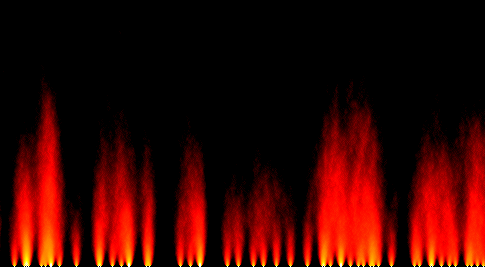
\includegraphics[width=8cm]{archivos/fire_final}
	\caption{Fuego dinámico, con intensidad por píxel aleatorizada}
	\label{fig:fire_final}
\end{figure}

\subsection{Resultado}

A continuación se presenta el resultado final del efecto de fuego: un fuego dinámico, de corte y comportamiento realista, con la posibilidad de cambiar su color y su intensidad.

\begin{figure}[h]
	\centering
	\begin{subfigure}[b]{0.3\textwidth}
		\centering
		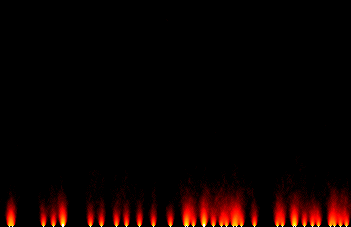
\includegraphics[width=4.5cm]{archivos/fire_final1}
		\caption{Fuego rojo con intensidad mínima}
		\label{fig:fire_final1}
	\end{subfigure}
	\begin{subfigure}[b]{0.3\textwidth}
		\centering
		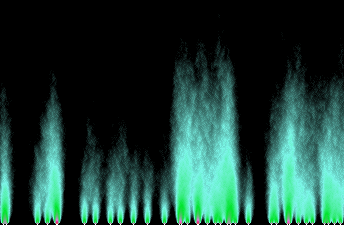
\includegraphics[width=4.5cm]{archivos/fire_final2}
		\caption{Fuego neón con intensidad media}
		\label{fig:fire_final2}
	\end{subfigure}
	\begin{subfigure}[b]{0.3\textwidth}
		\centering
		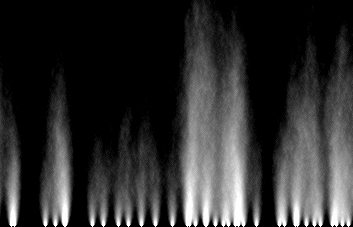
\includegraphics[width=4.5cm]{archivos/fire_final3}
		\caption{Fuego en blanco y negro con intensidad máxima}
		\label{fig:fire_final3}
	\end{subfigure}
\end{figure}

\section{Túnel de puntos}

\subsection{Investigación inicial}

Un efecto también muy común en el mundo de la \emph{demoscene} es el efecto de túnel o vórtice, entre otras causas por su relativa sencillez sumada a su espectacularidad (por la sensación de profundidad y de dinamismo, evocando a escenas futuristas o situadas en el espacio).\\

Es por ello que el efecto de túnel parecía un candidato perfecto para ser la segunda demo a implementar; más complejo que el efecto de fuego pero aún así sencillo, y con un resultado visual más complejo.\\

Una vez decidido, llegó el momento de recabar información acerca de este efecto y cómo implementarlo. Mi idea inicial era generar un túnel de puntos como el de la figura [\ref{fig:cyberdance}], sin embargo, conforme fui ahondando en mi búsqueda, descubrí que también era un efecto bastante común generar túneles como el que se muestra en la figura [\ref{fig:dane_kefrens}].\\ 

\begin{figure}[h]
	\centering
	\begin{subfigure}[b]{0.45\textwidth}
		\centering
		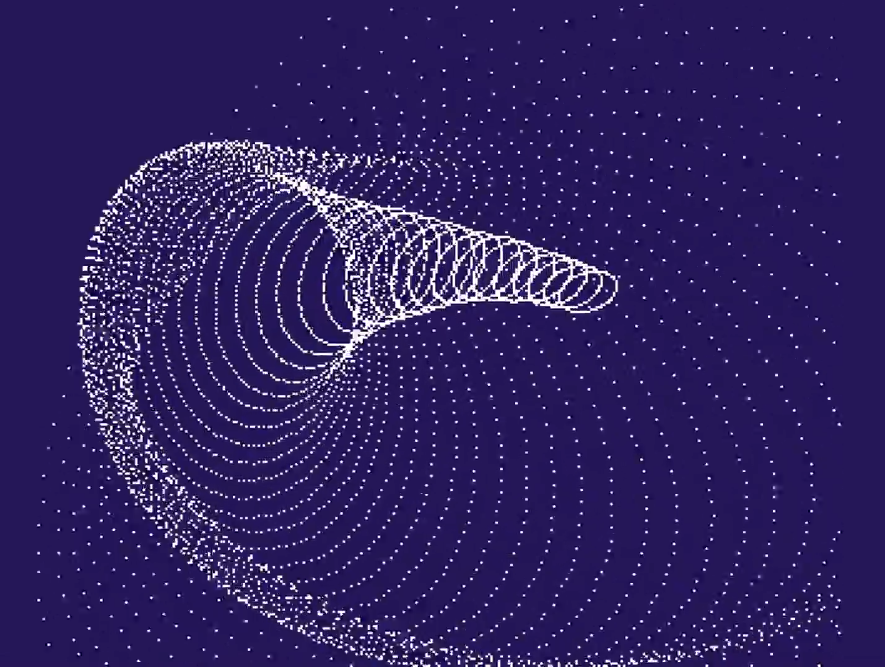
\includegraphics[width=6cm]{archivos/cyberdance}
		\caption{Túnel de puntos - Cyberdance (por Virtual Dreams y Fairlight, 1993) - Fuente: \href{https://www.youtube.com/watch?v=X7sHODKip_c}{YouTube}}
		\label{fig:cyberdance}
	\end{subfigure}
	\begin{subfigure}[b]{0.45\textwidth}
		\centering
		
\includegraphics[width=6cm]{archivos/dane_kefrens}
		\caption{Túnel mediante deformación de textura - D.A.N.E (por Kefrens, 1993) - Fuente: \href{https://www.youtube.com/watch?v=ZbPGU5p7O4Y}{YouTube}}
		\label{fig:dane_kefrens}
	\end{subfigure}
\end{figure}

De hecho, de cara a la búsqueda de explicaciones teóricas y detalles de implementación, fue más fácil encontrar información acerca del efecto mostrado en [\ref{fig:dane_kefrens}] que del túnel de puntos. Páginas como \emph{\href{http://benryves.com/tutorials/tunnel}{benryves.com}} o \emph{\href{https://lodev.org/cgtutor/tunnel.html}{lodev.org}} ofrecían tutoriales detallados, en los que se explica paso a paso la base matemática del efecto así como su implementación en código.\\

En resumen, el efecto que se muestra en la figura [\ref{fig:dane_kefrens}] es el resultado de deformar una imagen o una textura de forma que toda la textura tienda hacia un punto central, de modo que se produce una textura circular a partir de un patrón plano. Se deforma la imagen aplicando algo de trigonometría básica. Además, como en el ejemplo de \emph{\href{https://lodev.org/cgtutor/tunnel.html}{lodev.org}}, se pueden usar tablas precalculadas para así evitar tener que realizar operaciones trigonométicas complejas y/o lentas de forma repetida.\\

No fui, sin embargo, capaz de encontrar tutoriales o detalles de implementación para lograr el efecto de la figura [\ref{fig:cyberdance}]. Tras una búsqueda a conciencia con resultado infructuoso, me decidí por implementar este efecto. Mi objetivo con este trabajo no es el de seguir tutoriales ya existentes, si no el de crear efectos visuales partiendo de cero, y guiado por la intuición y la razón. No tiene sentido alguno que trate de implementar un efecto de túnel basado en una textura cuando ya hay tutoriales que desgranan (con detalle y acierto) cómo hacerlo, tanto a nivel matemático como de código.\\

Por tanto, resolví por implementar el efecto de túnel de puntos.

\subsection{Planteamiento formal}

¿Cómo se consigue el efecto de generar un túnel de puntos en movimiento?\\

La respuesta en realidad es bastante sencilla si observamos con atención cualquier demo que implemente este efecto: consiste en la superposición de circunferencias de distintos tamaños y en distintas posiciones. \\

El dibujado de estas circunferencias (o elipses en el caso de la figura [\ref{fig:cyberdance}]) se simplifica a dibujar solo varios puntos pertenecientes a la circunferencia, en lugar de dibujar todo el perímetro. De este modo se consigue un tiempo de dibujado controlable y constante (si decidimos que una circunferencia será representada mediante 16 puntos, se usarán 16 puntos ya sea el radio de la circunferencia 50, 100 o 200 píxeles, de modo que aunque el perímetro aumente, la esfera es representada con una cantidad de puntos constante -eso sí, cada vez más separados entre sí-).\\

Por tanto, será necesario implementar las siguientes funcionalidades:
\begin{itemize}
	\item Capacidad para dibujar un círculo dadas una posición, un radio y por cuantos puntos debe estar formado.
	\item Capacidad para mantener un conjunto de circunferencias simultáneamente
	\item Capacidad para gestionar el ciclo de vida de una circunferencia
	\item Implementar un mecanismo mediante el que el túnel siga una ruta de apariencia natural y fluida
\end{itemize}

\subsection{Implementación}

Empezando por el principio, era necesario poder dibujar circunferencias en pantalla. Estos círculos, además, debían poder variar su posición y tamaño a lo largo del tiempo, por lo que tenía sentido crear una estructura que los representara [\ref{fig:circleuml}].\\

%@startuml
%
%class Circle << (S,#FF7700) Struct >>
%{
%  +float x, y
%  +float radius
%}
%
%hide empty members
%
%@enduml

\begin{figure}[h]
	\centering
	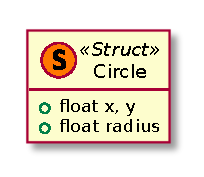
\includegraphics[width=6cm]{archivos/circleuml}
	\caption{Estructura básica de un círculo}
	\label{fig:circleuml}
\end{figure}

Como podemos ver en el código [\ref{cod:drawcircle}], para dibujar una circunferencia, lo que hacemos es ir de \(0\) a \(2 * \pi\). Esto es trazar una circunferencia completa en radianes. Definimos, no obstante, un incremento variable, que depende de la cantidad de puntos que queremos dibujar. De este modo, si queremos dibujar una circunferencia de 4 puntos, este incremento será \((2 \times \pi) \div 4 = \frac{\pi}{2}\), o lo que es lo mismo, dibujaremos de cuarto en cuarto de circunferencia, dibujando así 4 puntos para completar una circunferencia completa.\\

La operación para determinar la posición del punto es muy básica, e implica simplemente un poco de trigonometría. La posición de cada punto de la circunferencia viene determinada por el ángulo (por el coseno del mismo para la coordenada horizontal y por el seno para la coordenada vertical) multiplicado por el radio y sumada la posición del centro de la circunferencia.\\

Una vez obtenida la posición para un punto de la circunferencia, lo dibujamos usando nuestra función del motor para dibujar puntos, que se encarga además de comprobar que el punto esté dentro de los límites de pantalla, y nos permite además pasarle parámetros para el color y el tamaño del punto (blanco y de un píxel para el ejemplo).\\

\begin{lstlisting}[style=C-color, caption={Algoritmo básico de dibujado de circunferencias},label=cod:drawcircle]
void DotTunnelDemo::DrawCircle(const Circle &c)
{
    const float increment = (2 * Fast::PI) / float(pointsPerCircle);
    int x, y;

    for (float angle = 0, n = 2 * Fast::PI; angle < n; angle += increment)
    {
        x = cos(angle) * c.radius + c.x;
        y = sin(angle) * c.radius + c.y;
        
        RenderDot(x, y, Pixel(255), 1);
    }
}
\end{lstlisting}

Una vez podemos dibujar círculos, llega el momento de poder gestionar una serie de círculos y su ciclo de vida (creación, actualizaciones periódicas con radio creciente y destrucción alcanzado un cierto tamaño).\\

Para ello primero debemos preguntarnos, ¿cómo se comporta nuestro túnel? La respuesta es que para la estructura del túnel, lo que queremos es ir añadiendo nuevos círculos al principio del túnel y vamos eliminando los círculos que están al final del túnel cuando alcanzan cierto tamaño. Así pues, esta es una estructura FIFO (\emph{first-in, first-out}) o el primer elemento en crearse es el primer elemento en borrarse. Podríamos pensar que con usar una estructura de cola (\lstinline{std::queue}\footnote{\url{https://en.cppreference.com/w/cpp/container/queue}}) nos bastaría, sin embargo, una cola sólo permite crear un nuevo elemento al final de la estructura y borrarlo al principio, y además no permite el acceso a los elementos intermedios (que nosotros necesitamos para poder actualizarlos).\\

Por suerte, no obstante, hay una estructura similar que cumple todos los requisitos que necesitamos: \lstinline{std::deque}\footnote{\url{https://en.cppreference.com/w/cpp/container/deque}} (\emph{double-ended queue}). Aunque el nombre puede resultar algo extraño (cola con doble final), ¡esta estructura satisface coste constante para todas las operaciones que necesitamos! El coste de la inserción y borrado de elementos son constantes al principio y al final de la cola, y además el acceso aleatorio (acceso a un elemento cualquiera de la cola) es también constante. Por tanto, usaremos esta estructura para contener los círculos que formarán nuestro túnel.\\

\begin{lstlisting}[style=C-color, caption={Inserción y eliminación de círculos},label=cod:populatecirclequeue]
void DotTunnelDemo::PopulateCircleQueue()
{
    if (circles.front().radius > minCircleRadius)
    {
        circles.push_front(defaultCircle);
    }
    if (circles.back().radius > maxCircleRadius)
    {
        circles.pop_back();
    }
}
\end{lstlisting}

Como podemos ver en el código [\ref{cod:populatecirclequeue}], usando esta estructura es muy sencillo añadir y eliminar elementos de nuestro túnel. La lógica que seguimos es: si el último círculo que ha sido añadido alcanza cierto tamaño, entonces añadimos un nuevo círculo al túnel. Del mismo modo, cuando el círculo que más tiempo lleva en la cola alcanza cierto tamaño, es eliminado. Cabe notar que para añadir nuevas circunferencias a la cola, se hace una copia de una instancia que creamos en la inicialización del programa, y que contiene los valores de creación de un círculo por defecto. Además, para que este código funcione correctamente, debe haber al menos un elemento previamente insertado en la cola, es decir, no puede estar vacía. Es por eso que durante la inicialización de la demo también se añade un círculo a la cola, copiado de la instancia por defecto.\\

\begin{lstlisting}[style=C-color, caption={Actualización del túnel},label=cod:updatecirclequeue,escapechar=|]
void DotTunnelDemo::UpdateCircleQueue(float deltaTime)
{
    for (auto c : circles)
    {
        EraseCircle(c);|\label{line:erasecircle}|
    }

    PopulateCircleQueue();

    for (auto &c : circles)
    {
        UpdateCircle(c, deltaTime);|\label{line:updatecircle}|
        DrawCircle(c);
    }
}
\end{lstlisting}

Una vez que podemos dibujar círculos [\ref{cod:drawcircle}] y tenemos una estructura que representa nuestro túnel sobre la que podemos insertar y eliminar elementos [\ref{cod:populatecirclequeue}], llega el momento de dibujar nuestro túnel en pantalla, el proceso es bastante sencillo [\ref{cod:updatecirclequeue}].\\

Lo primero que hacemos es recorrer todos los círculos que conforman el túnel y borrarlos en pantalla, en la línea [\ref{line:erasecircle}]. Es importante notar que esta función no está eliminando los círculos de la cola, si no que simplemente \emph{borra en pantalla}. Internamente esta función llama a la función de dibujado [\ref{cod:drawcircle}] pero con una copia del círculo en color negro. Así, lo que hacemos al inicio de cada actualización es borrar los círculos \emph{que se dibujaron en el fotograma anterior}, previo a la actualización de los valores de los círculos. De este modo, en lugar de tener que poner a negro todos píxeles de la pantalla (que en alta definición son más de un millón), ponemos a negro sólo aquellos píxeles que fueron modificados en el fotograma anterior (que son cientos de píxeles, pero no miles o millones). Al borrar de este modo, se produce una gran optimización.\\

Tras haber borrado la pantalla, llamamos a la función [\ref{cod:populatecirclequeue}], que puede añadir o eliminar círculos del túnel si se cumplen las condiciones necesarias.\\

A continuación, actualizamos (línea [\ref{line:updatecircle}]) y redibujamos todos los círculos en pantalla. Actualmente, la actualización de un píxel es un proceso muy sencillo que consiste simplemente en ir aumentando el radio de cada círculo a lo largo del tiempo, en función de su radio anterior y una velocidad ajustable por el usuario (\lstinline{c.radius += c.radius * deltaTime * radiusVelocity;}).\{\\

El resultado de todo lo aplicado hasta ahora se puede ver en la figura [\ref{fig:basicdottunnel}].\\

\begin{figure}[h]
	\centering
	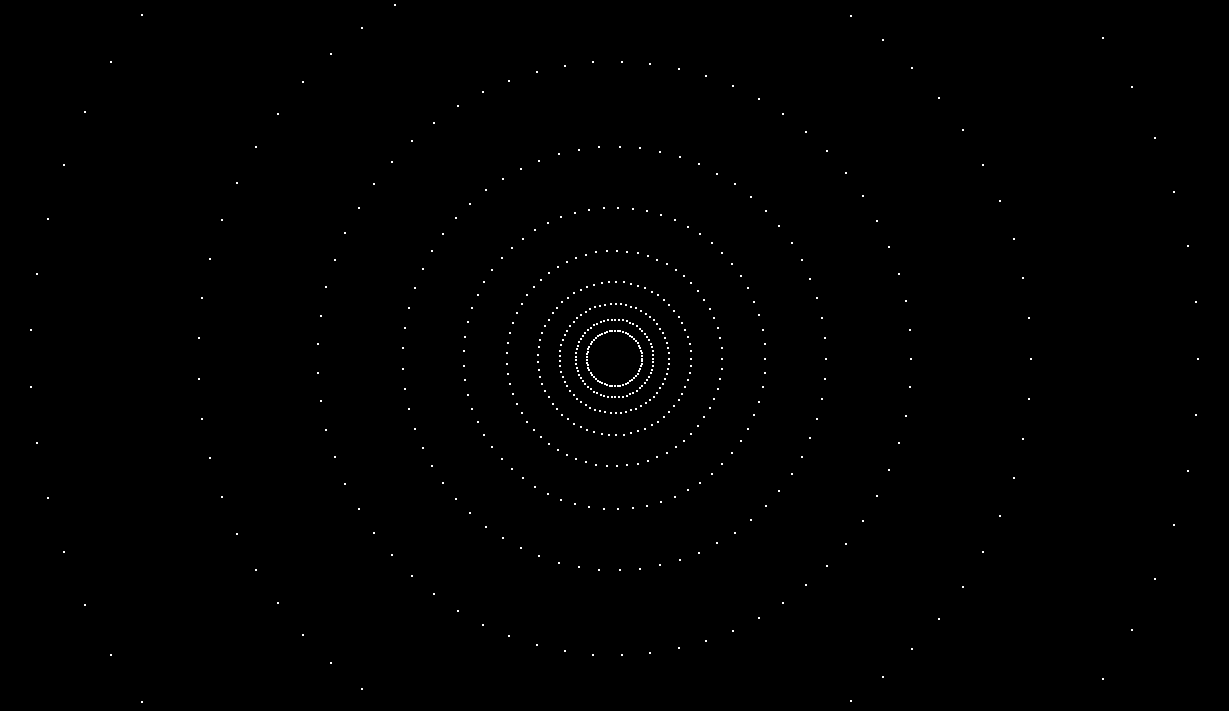
\includegraphics[width=10cm]{archivos/basicdottunnel}
	\caption{Túnel de puntos básico}
	\label{fig:basicdottunnel}
\end{figure}

Ahora todo lo que nos queda por hacer es dotar de movimiento al túnel, es decir, que no sólo los círculos aumenten de radio, si no que su posición también varíe. No obstante, no es necesario modificar la posición de los círculos una vez han sido creados, basta con que el centro de cada círculo esté desplazado en cuanto a posición con respecto al círculo anterior en su momento de creación. En otras palabras, cada círculo se crea en una posición distinta con respecto al punto de creación del círculo anterior, pero el centro del círculo no se modifica posterior a su creación. Aunque pueda resultar curioso, no es necesario mover el centro del círculo una vez creado, basta con ir haciendo el radio progresivamente más grande para crear una sensación de movimiento convincente.\\

Así pues, tan solo necesitamos crear cada círculo con una posición distinta pero coherente con respecto a la anterior, para dar sensación de continuidad. ¿Cómo podemos hacer esto?\\

No podemos decidir las direcciones de forma aleatoria, pues de este modo el movimiento no parecerá coherente. Cabe la posibilidad, no obstante, de seguir direcciones que se deciden aleatoriamente cada cierto tiempo, pero que se mantienen fijas durante un intervalo. Si hacemos esto el movimiento tendría coherencia pero aún así parecería poco natural cada vez que cambiáramos de dirección, pudiéndose producir cambios de dirección bruscos. Una posibilidad ante esto es interpolar la dirección actual con la dirección futura, de modo que los cambios de dirección queden suavizados. Pero aun así surge un problema más, no podemos controlar si el túnel se sale de los límites de la pantalla. Podríamos hacer entonces que si el túnel está cerca del límite de la pantalla, la nueva dirección elegida fuera hacia el centro de la pantalla. Aunque esto podría causar sensación de que cuando el túnel se acerca al límite de la pantalla rebota... Podríamos seguir con este modelo, a partir de direcciones o movimientos aleatorios, pues es factible, pero el código y la cantidad de situaciones con las que hay que lidiar para que el resultado parezca natural aumenta en  complejidad por momentos.\\

Fue por ello que cuando estaba pensando en cómo implementar este efecto, descarté esta opción. Pensando en otras opciones se me ocurrió la que sería la definitiva, construir un camino a partir de un punto que gira en torno a una "órbita" virtual que a su vez "orbita" en torno a otros puntos. Un poco de forma parecida a como orbitan los planetas, que si bien lo hacen bajo rutas perfectamente definidas, las combinaciones de órbitas a distintas velocidades dan resultado a trayectorias coherentes pero difíciles de predecir desde el punto de vista terráqueo [\ref{fig:cassini}].\\

\begin{figure}[h]
	\centering
	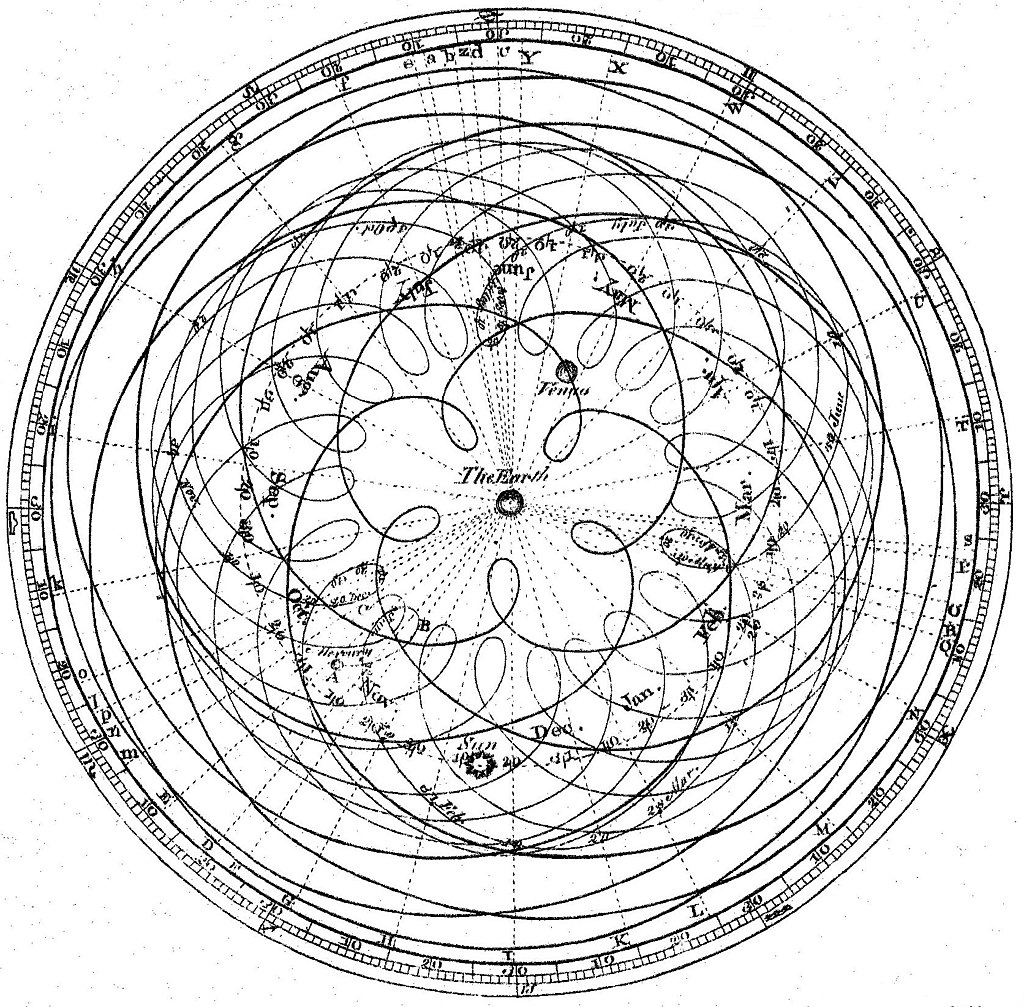
\includegraphics[width=8cm]{archivos/cassini}
	\caption{Órbitas de los planetas vistas desde la Tierra (por Giovanni Cassini) - Fuente: \href{https://es.wikipedia.org/wiki/Teoría_heliocéntrica\#/media/File:Cassini_apparent.jpg}{Wikipedia}}
	\label{fig:cassini}
\end{figure}

Así, con el modelo geocéntrico en mente, me dispuse a crear una clase que fuera capaz de emular este tipo de movimiento: controlado pero difícil de predecir.\\

Todo lo que necesitaba era un algoritmo que me devolviera un valor numérico entre -1 y 1 (al tener un rango controlado el túnel no podría salirse de pantalla) y se calculara como el resultado de la suma de distintos puntos rotando (o como la suma de ondas con distintas frecuencias, según el punto de vista). El resultado fue un algoritmo sencillo pero satisfactorio.\\

\begin{figure}[h]
	\centering
	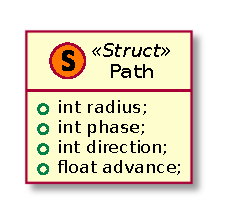
\includegraphics[width=6cm]{archivos/pathuml}
	\caption{Estructura de cada órbita que determina el camino}
	\label{fig:pathuml}
\end{figure}

Como podemos ver en la figura [\ref{fig:pathuml}], creamos una estructura sencilla que nos permite representar un punto orbitando. Un punto orbitando se ve definido por su radio de órbita, su fase (punto inicial en el que comienza a orbitar, la dirección en la que orbita -sentido horario o antihorario- y el avance o camino actual que el punto en órbita ha recorrido. Otras características como la velocidad de órbita se definen de forma global, y no por órbita, para nuestro ejemplo, aunque la velocidad de órbita viene condicionada por el radio de órbita.\\

\begin{lstlisting}[style=C-color, caption={Creación de un camino de turbulencia},label=cod:createturbulencepath,escapechar=|]
void TurbulencePath::CreateTurbulencePath(float pathVelocity, int pathRadius, int pathComplexity)
{
    this->pathVelocity = pathVelocity;
    this->pathRadius = pathRadius;
    this->pathComplexity = pathComplexity;

    for(int i = 0; i < pathComplexity; i++)
    {
        paths.push_back(Path{ |\label{line:createpath}|
                (pathRadius * 2) / (i + 2),
                Fast::Rand() * 2 * Fast::PI,
                i % 2 == 0 ? 1 : -1,
                0});
    }
}
\end{lstlisting}

En el código [\ref{cod:createturbulencepath}] podemos ver cómo podemos inicializar lo que definí como "camino de turbulencia". Para crear un "camino de turbulencia" necesitamos especificar la velocidad global que tendrá el camino, el mayor radio posible que el camino pueda generar, en píxeles, y la complejidad del camino, que es equivalente a la cantidad de órbitas (o ondas) superpuestas que formarán nuestro camino. En la línea [\ref{line:createpath}] podemos ver cómo añadimos caminos, la cantidad que añadimos dependiendo de la complejidad del mismo. Además, el radio de cada órbita depende de su orden (órbita 0 tendrá radio 1 (\(\frac{2}{2}\)), órbita 1 tendrá \(\frac{2}{3}\) del radio, órbita 2 tendrá \(\frac{1}{2}\) (\(\frac{2}{4}\)) del radio...). A continuación definimos la fase de forma aleatoria, la dirección (positiva para órbitas de orden par, negativas para impares) y el avance inicial, que es obviamente 0.\\

\begin{lstlisting}[style=C-color, caption={Actualización de un camino de turbulencia},label=cod:updateturbulencepath,escapechar=|]
void TurbulencePath::UpdateTurbulencePath(float deltaTime, float &pathX, float &pathY)
{
    pathX = 0.f;
    pathY = 0.f;

    for (auto& path : paths)
    {
        path.advance += deltaTime * 0.1;
        float waveFrequence = path.radius * pathVelocity;
        pathX += cos(waveFrequence * path.advance + path.phase);
        pathY += sin(waveFrequence * path.advance + path.phase);
    }

    pathX /= (float)pathComplexity; |\label{line:dividepath}|
    pathY /= (float)pathComplexity;

    pathX *= pathRadius; |\label{line:multiplypath}|
    pathY *= pathRadius;
}
\end{lstlisting}

Ahora llega el momento de ser capaces de actualizar nuestra estructura, como muestra el código [\ref{cod:updateturbulencepath}]. A esta función le pasamos el tiempo transcurrido desde el último fotograma y nos devuelve el punto actual en el que el camino se encuentra. Para ello, por cada camino, actualizamos el avance en función del tiempo y calculamos la frecuencia en función del radio y la velocidad del camino. Una vez hemos sumado todos los caminos, dividimos entre la complejidad (línea [\ref{line:dividepath}]) para normalizar el resultado (de este modo aseguramos que oscila entre -1 y 1). Tras ello, tan solo nos queda multiplicar el resultado normalizado por el radio del camino para obtener el punto en el que nos hallamos actualmente (línea [\ref{line:multiplypath}]).\\

Una vez tenemos nuestro "camino de turbulencia" creado, tan solo tenemos que incorporarlo en nuestro código del túnel e ir actualizándolo periódicamente. Para ello, modificamos la función \lstinline{PopulateCircleQueue()} [\ref{cod:populatecirclequeue}] para que cada vez que añadamos un círculo, desplacemos su centro por la posición actual del "camino de turbulencia".\\

Podemos ver el resultado en la figura [\ref{fig:tunnelwithturbulence}].

\begin{figure}[h]
	\centering
	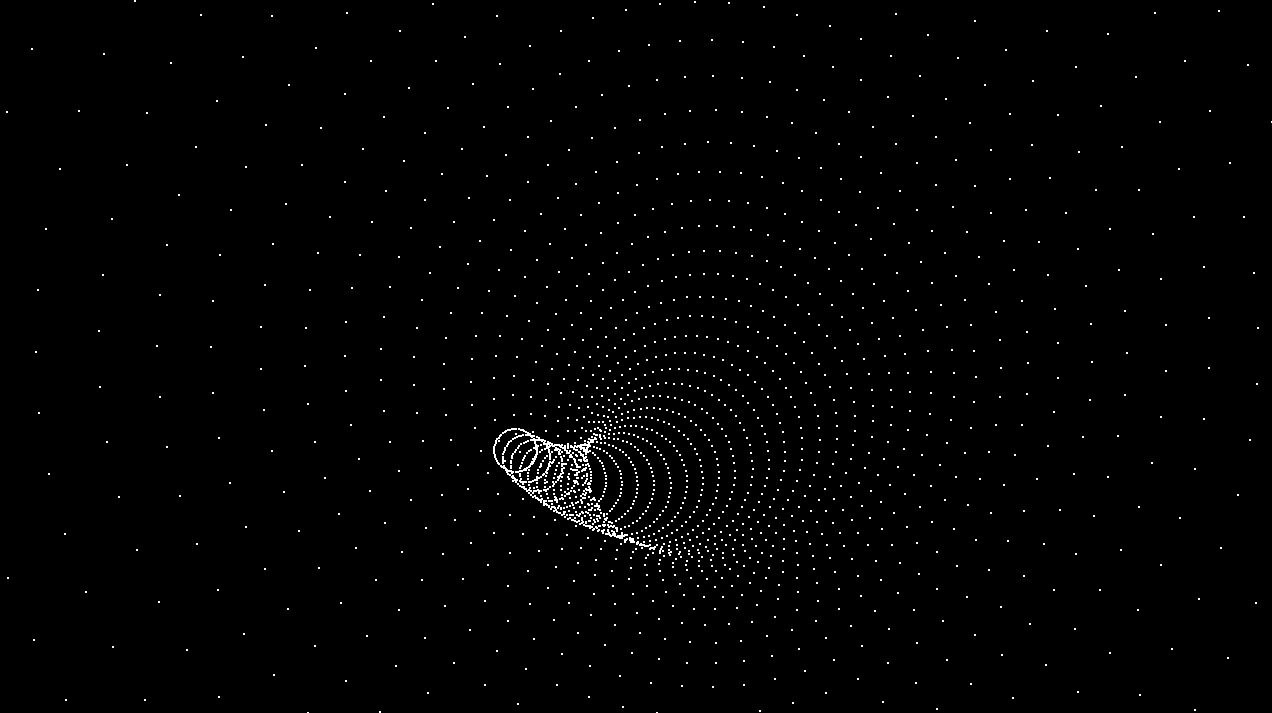
\includegraphics[width=10cm]{archivos/tunnelwithturbulence}
	\caption{Tunel básico siguiendo un camino}
	\label{fig:tunnelwithturbulence}
\end{figure}

\subsection{Refinamiento}

Una vez tenemos nuestro efecto de túnel acabado, llega el momento de iterar sobre la idea para mejorar el resultado, tanto a nivel visual como de rendimiento. A continuación se exponen las medidas que se tomaron:

\begin{itemize}
	\item \textbf{Sustituir operaciones trigonométricas por tablas precalculadas}: como pudimos comprobar con los tests de rendimiento, las operaciones trigonométricas tienen un coste de computación alto. En esta demo hacemos un uso periódico de operaciones de seno y coseno, para calcular la posición de cada punto del túnel, así como para el camino de turbulencia. Si en lugar de usar funciones trigonométricas de forma directa, usamos tablas precalculadas, el coste de estas operaciones pasará a ser el de un acceso constante. No obstante, como todo, usar tablas precalculadas tiene también su coste. La principal ventaja de usar tablas precalculadas es la eficiencia, no obstante lo hacemos al coste de complejidad espacial (tenemos que guardar cada valor precalculado en memoria, y las tablas pueden llegar a ser bastante grandes), pérdida de precisión (al ser valores precalculados, solo podemos acceder a aquellos que hemos calculado, no siendo posible acceder a valores intermedios) y aumento en la complejidad del código (en lugar de pasar un valor en radianes a una función, debemos calcular a partir de un ángulo el índice de acceso a la tabla para el valor que queremos).
	
	Podría parecer, dadas las desventajas listadas, que no vale la pena esta optimización. Esto es siempre una cuestión de interpretación y de límites, y depende de la situación y del sistema en que nos encontremos. En nuestro caso concreto, la memoria no es un limitante (disponemos de gigabytes de memoria RAM) pero sin embargo la CPU sí lo es (tenemos que operar sobre grandes cantidades de valores en intervalos muy cortos de tiempo -cientos o miles de píxeles por fotograma-). Por tanto, vale la pena aumentar la complejidad del código a cambio de que sea notablemente más eficiente.
	
	Como podemos ver en el código [\ref{cod:generatesinetable}], crear una tabla precalculada es más bien sencillo. En este caso, por simplicidad se ha decidido que las tablas se calculan de forma dinámica al inicio de la ejecución de la aplicación, tomando solo así tiempo de cálculo durante la inicialización. No obstante, hubiera sido posible también implementar este mismo mecanismo mediante el uso de \emph{templates} y \emph{constexpr}\footnote{\url{https://en.cppreference.com/w/cpp/language/constexpr}}. De este modo se podría hacer que las tablas se calculasen en tiempo de compilación, embebiéndose la tabla precalculada en el propio código del programa, no tomando así ningún tiempo de cálculo en ejecución. Se ha decido crear las tablas de forma dinámica, no obstante, por simplicidad de código y reducción de los tiempos de compilación.
	
	Así pues, en el código [\ref{cod:generatesinetable}] vemos como para crear una tabla, tan sólo debemos pasarle un tamaño y nos devolverá una tabla del tamaño dado, conteniendo valores incrementales para el seno en una circunferencia completa (de 0 a \(2 \times \pi\) radianes). Hay que tener en cuenta que la precisión de la tabla es equivalente al tamaño de la misma (a mayor tamaño, mayor precisión, pero también ocupa más espacio en memoria y tarda más en calcularse).
	
	En la línea [\ref{line:drawcircle}] podemos ver el resultado de usar nuestras tablas precalculadas en lugar de operaciones trigonométricas de forma directa, como en [\ref{cod:drawcircle}]. Como podemos ver, la complejidad del código aumenta ligeramente, aunque eso sí, a cambio de poder obtener valores de operaciones complejas en tiempo constante. Para ello, necesitamos calcular un factor (línea [\ref{line:indexFactor}]) que nos permita marcar una correspondencia entre el ángulo que queremos y el índice que corresponde en la tabla. Luego, para acceder al valor del coseno (línea [\ref{line:cosinetable}]), multiplicamos el valor del ángulo que queremos por el factor calculado en la línea [\ref{line:indexFactor}]. Convertimos el resultado de esta operación en un entero (el acceso a memoria debe hacerse mediante un valor entero, pues la memoria es discreta, no se puede acceder a "medio bit"), lo que trunca el resultado y lleva a la consiguiente pérdida de precisión. A continuación hallamos el módulo en función del tamaño de la tabla. De este modo, si nos salimos del rango de la tabla, simplemente volvemos a inicio de la misma, de forma circular, por lo que no es posible de forma efectiva salirse de rango.
	
	De este modo, conseguimos una gran optimización (operaciones trigonométricas con coste constante equivalente a un acceso aleatorio). Esta optimización puede no hacerse tan evidente en tiempo de ejecución en esta demo, donde trabajamos con cientos o miles de píxeles, pero sin llegar al orden del millón, pero será crucial en futuras demos, para conseguir una tasa de actualización de fotogramas estable y fluida.

	\item \textbf{Añadir colores al túnel}: añadir colorido al túnel es muy sencillo, y sin embargo, mejora notablemente el resultado final. Basta con añadir a nuestro modelo de círculo [\ref{fig:circleuml}] un campo para el color, de modo que en lugar de estar predefinido a blanco, el color con el que se dibuja cada círculo dependa del propio círculo. De este modo, podemos crear un degradado de color, como los que ya creamos para el efecto de fuego, y asignar un nuevo color a cada círculo que creamos, basándonos en los valores del degradado. Para esta demo en concreto, hemos decidido crear una gama de colores de efecto \emph{arcoiris}.
	
	\item \textbf{Fundido de entrada y de salida}: en el estado actual de la demo, cuando un círculo se crea aparece de golpe y cuando un círculo se elimina desaparece de golpe. Teniendo en cuenta que actualmente el túnel es fluido tanto a nivel de movimiento (gracias al "camino de turbulencia") como a nivel de color (gracias al uso de un degradado), que los círculos aparezcan y desaparezcan de golpe rompe esta fluidez. Esto es muy sencillo de solucionar, añadiendo un fundido de entrada (opacidad creciente) cuando añadimos un nuevo círculo al túnel y un fundido de salida (opacidad decreciente) cuando estamos cerca de eliminar un círculo. De este modo, basta con crear un método que cumpla la siguiente función:
	
	\begin{itemize}
		\item Cuando un círculo se añade, el valor de la opacidad es 0, y crece gradualmente hasta uno conforme el radio del círculo incrementa
		\item Durante todo el ciclo de vida del círculo la opacidad es 1
		\item Cuando el radio del círculo se acerca al radio máximo (radio que una vez alcanzado, el círculo es eliminado) empezamos a decrementar el valor de la opacidad, de modo que sea 0 cuando el círculo sea eliminado.
	\end{itemize}
	
	De este modo, tan solo tenemos que multiplicar el valor de la opacidad por el color del círculo para conseguir nuestros fundidos de entrada y de salida, suavizando así la creación y eliminación de los círculos.
	
	\item \textbf{Rotación}: actualmente todos los círculos tienen la misma fase inicial (0), de modo que están alineados. Modificando la fase inicial para que se incremente en función del valor del tiempo de vida el círculo, en la función \lstinline{UpdateCircle()}\{, conseguimos que los círculos dejen de estar alineados y tengan una rotación propia, lo que da un cierto efecto de succión o de torbellino al túnel, lo que favorece el resultado visual.
	
	\item \textbf{Control por parte del usuario}: podemos hacer que el túnel sea modificable por el usuario haciendo simplemente que varias variables que ya tenemos se vean alteradas por determinadas entradas de teclado, por ejemplo:
	
	\begin{itemize}
		\item \textbf{Velocidad del túnel}: modificando la variable \emph{radiusVelocity}, que incrementa la velocidad de crecimiento de los círculos
		\item \textbf{Tamaño de los puntos}: nuestra función para dibujar puntos tiene la capacidad para recibir un tamaño, tan solo debemos usar esto en nuestro favor para añadir una variable modificable que contenga el tamaño de los puntos
		\item \textbf{Posición del centro del túnel}: si modificamos el centro del túnel, tenemos la sensación de poder \emph{controlar} el túnel.
	\end{itemize}
	
	De este modo, podemos con modificaciones muy pequeñas hacer que nuestra demo sea ampliamente interactiva. Luego, basta con utilizar la funcionalidad para dibujar texto para comunicar las instrucciones de uso al usuario.
	
\end{itemize}

\begin{lstlisting}[style=C-color, caption={Generación de tablas precalculadas y uso en código}, label=cod:generatesinetable, escapechar=|]
float *Fast::GenerateSineTable(int size)
{
    float *sineTable = new float[size];

    for (int i = 0; i < size; i++)
    {
        float value = (i * 2 * Fast::PI) / size;
        sineTable[i] = sin(value);
    }

    return sineTable;
}

void DotTunnelDemo::DrawCircle(const Circle &c)|\label{line:drawcircle}|
{
    const float increment = (2 * Fast::PI) / float(pointsPerCircle);
    const int indexFactor = mathTableSize / (2 * Fast::PI);|\label{line:indexFactor}|
    int x, y;

    for (float angle = 0, n = 2 * Fast::PI; angle < n; angle += increment)
    {
        x = cosineTable[int(angle * indexFactor) % mathTableSize] * c.radius + c.x; |\label{line:cosinetable}|
        y = sineTable[int(angle * indexFactor) % mathTableSize] * c.radius + c.y;
        
        RenderDot(x, y, Pixel(255), 1);
    }
}
\end{lstlisting}

\subsection{Resultado}

En la figura [\ref{fig:finaltunnel}] podemos ver el resultado final de nuestro túnel. Sigue un camino turbulento, se le aplica un degradado de color, los círculos tienen fundido de entrada y de salida y rotan, creando una sensación de vórtice.\\

Además, el tamaño de los puntos, la posición del centro del túnel y la velocidad del mismo son controlables por el usuario (las instrucciones no se muestran en la figura para no añadir ruido visual al resultado).\\
 
La demo además usa tablas precalculadas para evitar tener que realizar costosas operaciones trigonométricas (la diferencia en el resultado es apenas visible, aunque prestando atención es posible notar irregularidades entre la distancia de algunos puntos -este error se podría mitigar aumentando el tamaño de la tabla, y por tanto su resolución-). 

\begin{figure}[h]
	\centering
	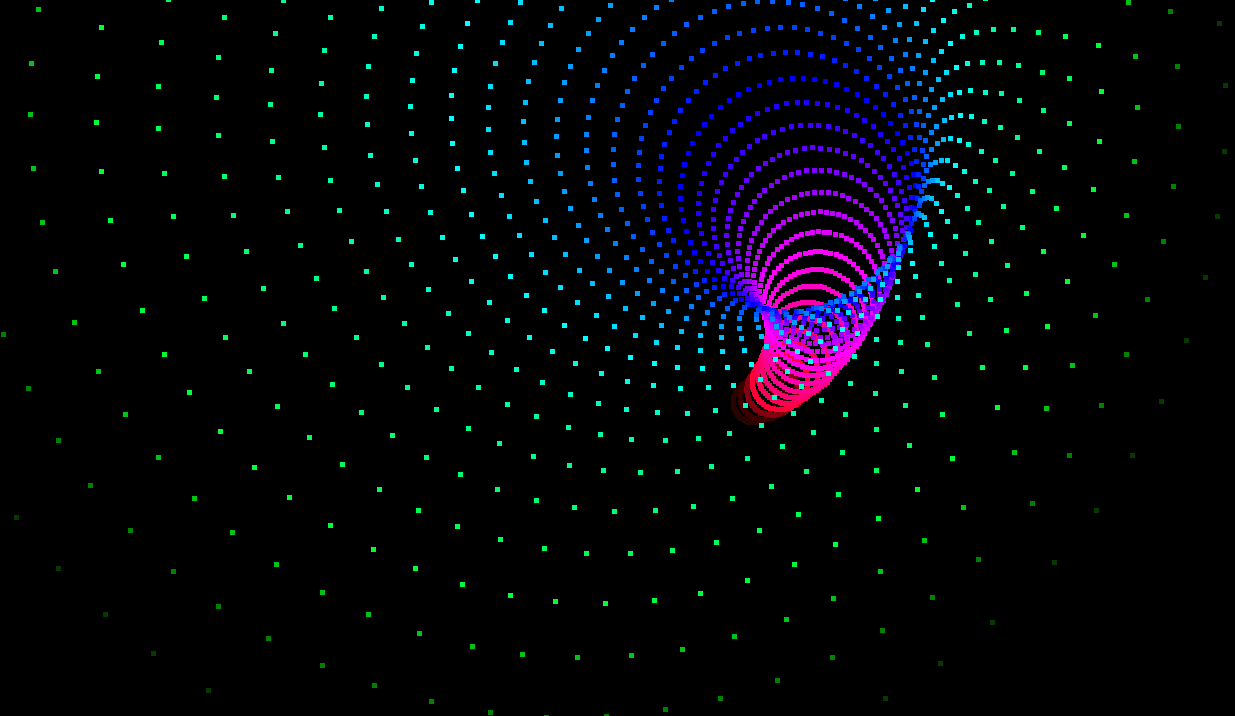
\includegraphics[width=12cm]{archivos/finaltunnel}
	\caption{Túnel final}
	\label{fig:finaltunnel}
\end{figure}

\section{RotoZoom}

\subsection{Investigación inicial}

El efecto de \emph{RotoZoom} es otro de los grandes clásicos de la \emph{demoscene}, y su nombre es bastante autodescriptivo. El efecto de \emph{RotoZoom} consiste en una imagen que se rota y escala en tiempo real. Podemos ver un ejemplo del mismo en la famosa demo \emph{Second Reality} [\ref{fig:second-reality-rotozoom}].\\

Existe amplia documentación para la implementación de este efecto, que además, es muy sencillo, pues se trata simplemente de transformaciones geométricas sencillas en el espacio 2D, dónde el grueso del algoritmo reside en transformar coordenadas en función de una rotación y escala variables.\\

\begin{figure}[h]
	\centering
	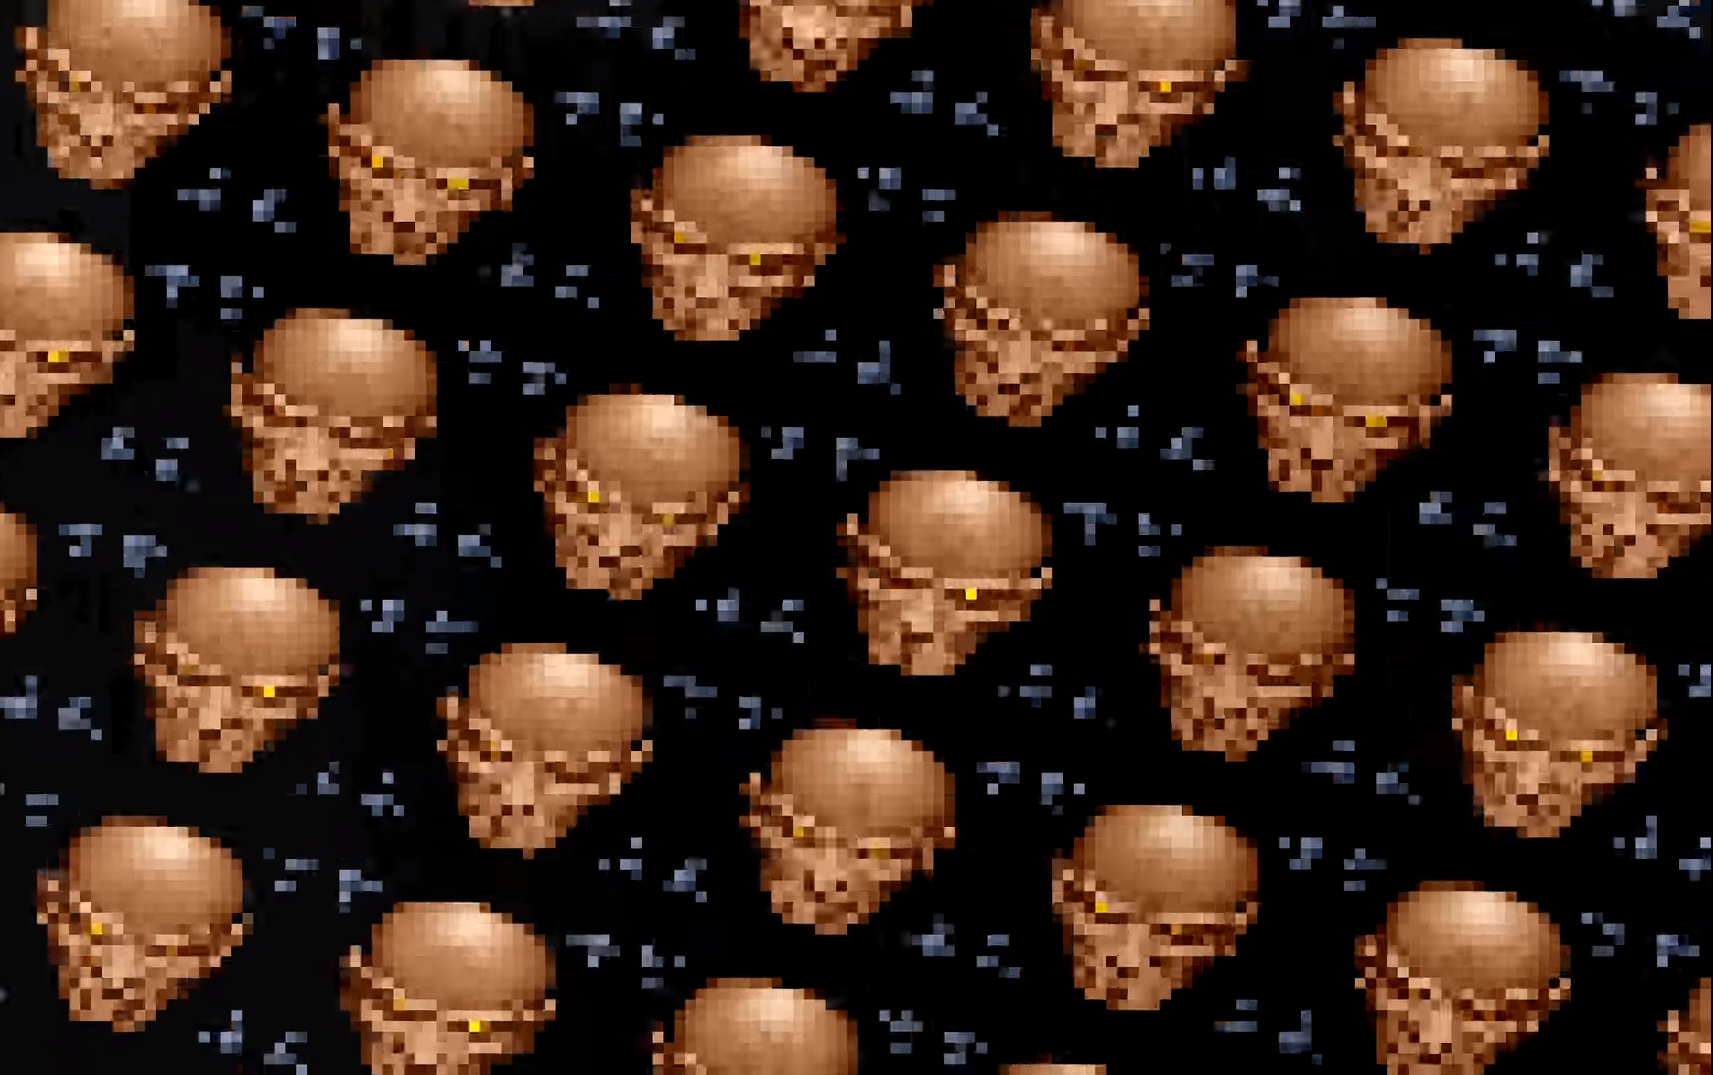
\includegraphics[width=8cm]{archivos/second-reality-rotozoom}
	\caption{Efecto de RotoZoom - Second Reality (by Future Crew) - Fuente: \href{https://www.youtube.com/watch?v=rFv7mHTf0nA&t=5m6s}{YouTube}}
	\label{fig:second-reality-rotozoom}
\end{figure}

\subsection{Planteamiento formal}

En la figura [\ref{fig:transform}] podemos ver las tranformaciones necesarias en el espacio bidimensional para escalar, rotar y trasladar un vector o un punto. Además, se dan también las operaciones matématicas necesarias para hacerlo. Aparece para cada transformación, en rojo el vector inicial y en granate el vector transformado. El orden de las operaciones de escalado y rotación en el ejemplo son intercambiables, es decir, el resultado de la transformación no se verá alterado por qué operación se realice antes. La traslación, no obstante, siempre debe ser la última operación que se realice (ya que el escalado y la rotación son consistentes cuando se realizan en torno al origen, pero no son conmutativas si el centro se ve desplazado).\\

\begin{figure}[h]
	\centering
	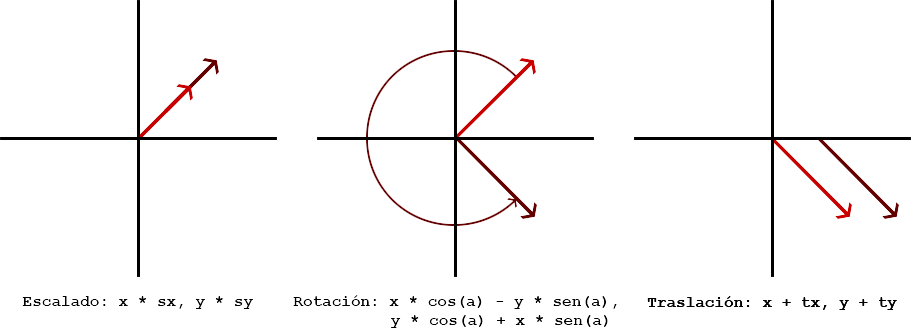
\includegraphics[width=14cm]{archivos/transform}
	\caption{Escalado, rotación y traslación en el espacio 2D}
	\label{fig:transform}
\end{figure}

El algoritmo principal para realizar este efecto será, por tanto, sencillo. No obstante, debemos tener algo en cuenta. Este algoritmo lo aplicaremos sobre una \textbf{imagen} y actualmente, no tenemos modo alguno de cargar imágenes en nuestras demos, por lo que tendremos que añadir esta funcionalidad.\\

Por tanto, deberemos seguir los siguientes pasos:
\begin{itemize}
	\item Implementar un modo de cargar imágenes en nuestra demo
	\item Realizar transformaciones geométricas sencillas para emular el efecto de rotación y escalado
\end{itemize}

\subsection{Implementación}

Lo primero que necesitamos hacer es tener un modo de cargar imágenes en nuestro sistema. Siguiendo con la filosofía de este trabajo, intentamos minimizar el uso de librerías externas al máximo, intentando implementar desde cero todo aquello que esté dentro de un ámbito razonable. La \emph{standard library} de C++ nos ofrece funcionalidades para manejar ficheros binarios, por lo que podremos usarlas para hacer nuestro trabajo más sencillo. No obstante, necesitaremos interpretar el fichero cargado en memoria para que una cadena de bytes en memoria pase a convertirse en una imagen que podemos manipular.\\

Es por ello que lo primero que cabe preguntarse es: ¿qué formato de imagen debemos emplear? Para no salir del ámbito de este trabajo, debemos elegir un formato que sea sencillo de leer y manipular, y este es sin duda, BMP, un formato de imagen sin transparencia ni compresión. En Wikipedia se ofrece una explicación en profundidad del formato BMP \footnote{\url{https://en.wikipedia.org/wiki/BMP_file_format}}, que nos será muy útil para saber cómo interpretarlo.\\

Estas son las consideraciones que tendremos en cuenta para nuestra cargar de imágenes en BMP, a partir de un archivo binario cargado en memoria:

\begin{itemize}
	\item Necesitamos saber la anchura de la imagen, que se puede encontrar en el byte 18 del fichero BMP y ocupa 4 bytes, en \emph{little-endian}
	\item Necesitamos saber la altura de la imagen, que se puede encontrar en el byte 22 del fichero BMP y ocupa 4 bytes, en \emph{little-endian}
	\item Asumimos que la profundidad de color será de 24 bits por píxel (1 byte por color)
	\item Asumimos que no hay ningún tipo de compresión
	\item En el formato BMP cada fila de la imagen está alineada a 32 bits
	\item En el formato BMP, la imagen está guardada de abajo a arriba y de izquierda a derecha (es decir, por filas, empezando en la inferior)
\end{itemize}

%@startuml
%
%class FileLoader
%{
%  +OpenBinaryFile(in path, out file, out size)
%  +CloseBinaryFile(in file)
%}
%
%class BMP
%{
%  +OpenRGBImage(in path, out image, out width, out height)
%  +CloseRGBImage(in image)
%  -CharToInt(in pointerToCharArray)
%}
%
%hide empty members
%
%BMP -> FileLoader : "uses"
%
%@enduml

\begin{figure}[h]
	\centering
	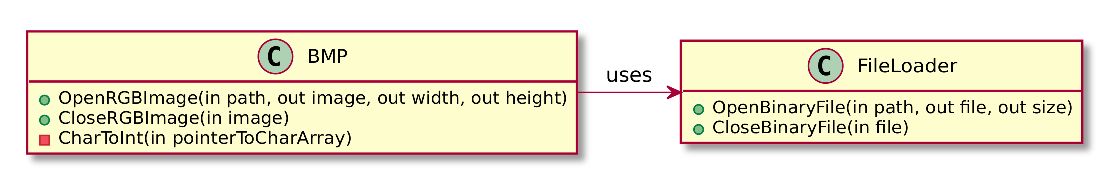
\includegraphics[width=14cm]{archivos/bmpuml}
	\caption{Diagrama del sistema para cargar imágenes}
	\label{fig:bmpuml}
\end{figure}

Como podemos ver en la figura [\ref{fig:bmpuml}], nos ayudaremos de una clase a la que hemos llamado \emph{FileLoader} a la que simplemente pasaremos una cadena de texto con la ubicación de la imagen que queremos abrir y nos devolverá una copia del fichero (como una cadena de bytes \lstinline{unsigned char *}\{) y el tamaño en bytes del mismo. Para realizar estas operaciones, nos ayudamos de la librería \emph{fstream} de la \emph{standard library}.\\

Nuestra clase principal, \emph{BMP} [\ref{fig:bmpuml}], convertirá la cadena de bytes (\lstinline{unsigned char *}\{) que recibe del \emph{FileLoader} en una cadena de píxeles (\lstinline{Pixel *}\{) usable por nuestras demos.\\

\begin{lstlisting}[style=C-color, caption={Código para cargar una imagen BMP en nuestro sistema}, label=cod:openrgbimage, escapechar=|]
void BMP::OpenRGBImage(const char *path, Pixel *&image, int &width, int &height)
{
    unsigned char *imageBinary = nullptr;
    unsigned int imageSize;

    FileLoader::OpenBinaryFile(path, imageBinary, imageSize);

    width = CharToInt(imageBinary + 18);  //Offset where width info is in BMP format
    height = CharToInt(imageBinary + 22); //Offset where height info is in BMP format
    image = new Pixel[width * height]; |\label{line:pixeltexture}|

    for (int j = 0; j < height; j++)
    {
        for (int i = 0; i < width; i++)
        {
            //The first part of the index "(imageSize - (j + 1) * width * 3) + i * 3" 
            //draws the image inverted in the Y axis
            //The second part of the index "- ((width * 3) % 4) * j" 
            //adds the corresponding offset (in the BMP format
            //All rows are 32 bit aligned)
            int index = (imageSize - (j + 1) * width * 3) + i * 3 - ((width * 3) % 4) * j; |\label{line:bmpindex}|
            image[j * width + i] = Pixel(imageBinary[index + 2], imageBinary[index + 1], imageBinary[index]);
        }
    }

    FileLoader::CloseBinaryFile(imageBinary);
}
\end{lstlisting}

Aunque el código [\ref{cod:openrgbimage}] pueda parecer algo complejo, en realidad es bastante sencillo. Una vez tenemos un puntero a nuestro archivo binario, que sabemos que será un fichero BMP, lo primero que hacemos es obtener la altura y anchura de la imagen a leer. Como sabemos la posición en la que se encuentran la anchura y la altura, dado que vienen especificadas por el formato, tan solo tenemos que acceder directamente a la posición donde se encuentran los bytes que nos interesan e interpretarlos. Es por ello que necesitamos una función que sea capaz de, a partir de una dirección de memoria dada, leer 4 bytes que representan un entero de 32 bits en \emph{little-endian}\footnote{\url{https://en.wikipedia.org/wiki/Endianness\#Little-endian}} y devolver como resultado un entero [\ref{cod:chartoint}]. Logramos este resultado mediante el uso de operaciones a nivel de bit, creando una correspondencia byte a byte entre nuestra cadena de bytes y nuestro entero.\\

\begin{lstlisting}[style=C-color, caption={Código para convertir una cadena de 4 bytes en un entero de 32 bits}, label=cod:chartoint]
int BMP::CharToInt(unsigned char *p)
{
    int number = 0;

    number = p[0];
    number = number | p[1] << 8;
    number = number | p[2] << 16;
    number = number | p[3] << 24;

    return number;
}
\end{lstlisting}

Una vez hemos obtenido de las cabeceras de nuestro fichero BMP la anchura y altura de la imagen a procesar, en píxeles, podemos calcular el tamaño de nuestra textura e inicializar una textura formada por nuestros píxeles, como podemos ver en la línea [\ref{line:pixeltexture}]. Ahora, debemos rellenar nuestra recién creada textura de un modo que sea fácilmente manipulable en nuestro sistema. Para ello, tenemos que tener en cuenta que el formato BMP incluye la información fila a fila de abajo arriba, por lo que nosotros tendremos que invertirla, para poder tratar nuestra imagen de forma más cómoda, de arriba abajo. Además, tenemos que tener en cuenta que los píxeles están alineados a 32 bits por cada fila. Como podemos ver en la figura [\ref{fig:pixelalignment}], en una imagen de 5x4 píxeles, el formato BMP incluiría un byte extra por fila, de modo que las filas estén siempre alineadas a 32 bits. En la figura [\ref{fig:pixelalignment}], cada celda representa un byte, cada grupo de color (gris o blanco) representa un píxel (tres bytes) y el color rojo representa los bytes añadidos al final de cada fila para que la memoria esté alineada a 32 bits (4 bytes).\\

\begin{figure}[h]
	\centering
	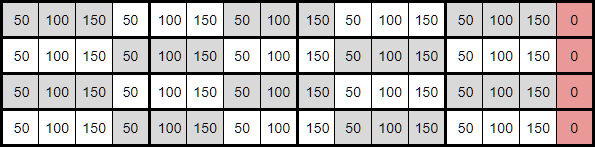
\includegraphics[width=12cm]{archivos/pixelalignment}
	\caption{Representación de los píxeles para una imagen 5x4 en BMP}
	\label{fig:pixelalignment}
\end{figure}

Es por ello que si bien rellenamos nuestra textura de arriba abajo, de izquierda a derecha y de forma lineal, en la línea [\ref{line:bmpindex}] calculamos un índice que accede a nuestro fichero BMP de abajo arriba, de izquierda a derecha y saltando al final de cada  fila (evitando introducir datos basura que se usan para mantener el alineamiento por fila).\\

Tras ello, nos aseguramos de liberar la memoria correspondiente y ¡ya hemos convertido nuestra imagen BMP a un formato manejable en nuestras demos!\\

Ahora tan solo queda implementar el algoritmo de \emph{RotoZoom}, lo cual resulta bastante trivial, como podemos ver en el código [\ref{cod:drawrotozoom}]. Para hallar la posición de la textura que corresponde a nuestro píxel, aplicamos primero una rotación, tras ello un escalado y por último, sumamos un desplazamiento. Cabe denotar que para mantener la coherencia de los resultados, nos quedamos con el valor absoluto de la transformación y le aplicamos el módulo en función del tamaño de la textura, para evitar que nuestro píxel se salga de los límites de la textura.\\

\begin{lstlisting}[style=C-color, caption={Dibujar un píxel cuya textura se desplaza en función de un ángulo, una escala y una traslación}, label=cod:drawrotozoom]
void RotoZoom::DrawPixel(int x, int y, int offsetX, int offsetY, int angle, float scale)
{
    int texX = Fast::Abs(int((x * cos(angle) - y * sin(angle)) * scale + offsetX)) % texWidth;
    int texY = Fast::Abs(int((y * cos(angle) + x * sin(angle)) * scale + offsetY)) % texHeight;

    pixels[y * width + x] = texture[texY * texWidth + texX];
}
\end{lstlisting}

Una vez aplicada esta transformación, ¡nuestro efecto de \emph{RotoZoom} está acabado! Y con una tasa de fotogramas de nada más y nada menos que \textbf{5 fotogramas por segundo}...

\subsection{Refinamiento}

Como vimos en los tests de rendimiento y como hemos mencionado en el análisis de la demo del Túnel de puntos, las operaciones con funciones matemáticas son costosas. \textbf{Muy costosas}. Si operamos tan solo con unos pocos píxeles no hay problema, pero si debemos iterar sobre cada uno de los píxeles en pantalla, que en nuestro caso son más de un millón... resulta inviable.\\

El primer cambio que podemos hacer, si nos fijamos en el código [\ref{cod:drawrotozoom}], es extraer el resultado del seno y el coseno a una variable, ya que se realiza la misma operación dos veces. Únicamente hacer esto ya duplicará la velocidad de fotogramas, a 10 fotogramas por segundo, lo cual sigue siendo inaceptable.\\

Por suerte, y con previsión, ya hemos implementado un método para generar tablas precalculadas [\ref{cod:generatesinetable}]. Si en lugar de usar funciones matemáticas usamos valores precalculados, nuestra tasa de fotogramas aumenta a \textbf{28 por segundo} en modo \emph{debug} y \textbf{40 fotogramas por segundo} en modo \emph{release}, las cuales ya se pueden considerar tasas de fotogramas aceptables, dado que el ojo humano percibe continuidad a partir de algo más de 12 fotogramas por segundo\footnote{\url{https://es.wikipedia.org/wiki/Fotogramas_por_segundo}}.\\

Ahora que tenemos una tasa de fotogramas adecuada y estable, llega el momento de crear una sensación de movimiento que parezca aleatorio pero continuo y fluido... por suerte, este también es un problema que se repite, pues es el mismo problema que teníamos con la ruta que debía seguir el "túnel de puntos". Así que podemos reutilizar la solución, ajustando valores. Así pues, creamos un "camino de turbulencia" que controlará los valores \emph{x} e \emph{y} de nuestra traslación y otro que controlará los valores del ángulo y la escala.\\

De este modo, las transformaciones que aplicamos sobre nuestros píxeles tendrán un efecto continuo y fluido, pero con una ruta impredecible.\\

\subsection{Resultado}

\begin{figure}[h]
	\centering
	\begin{subfigure}[b]{0.48\textwidth}
		\centering
		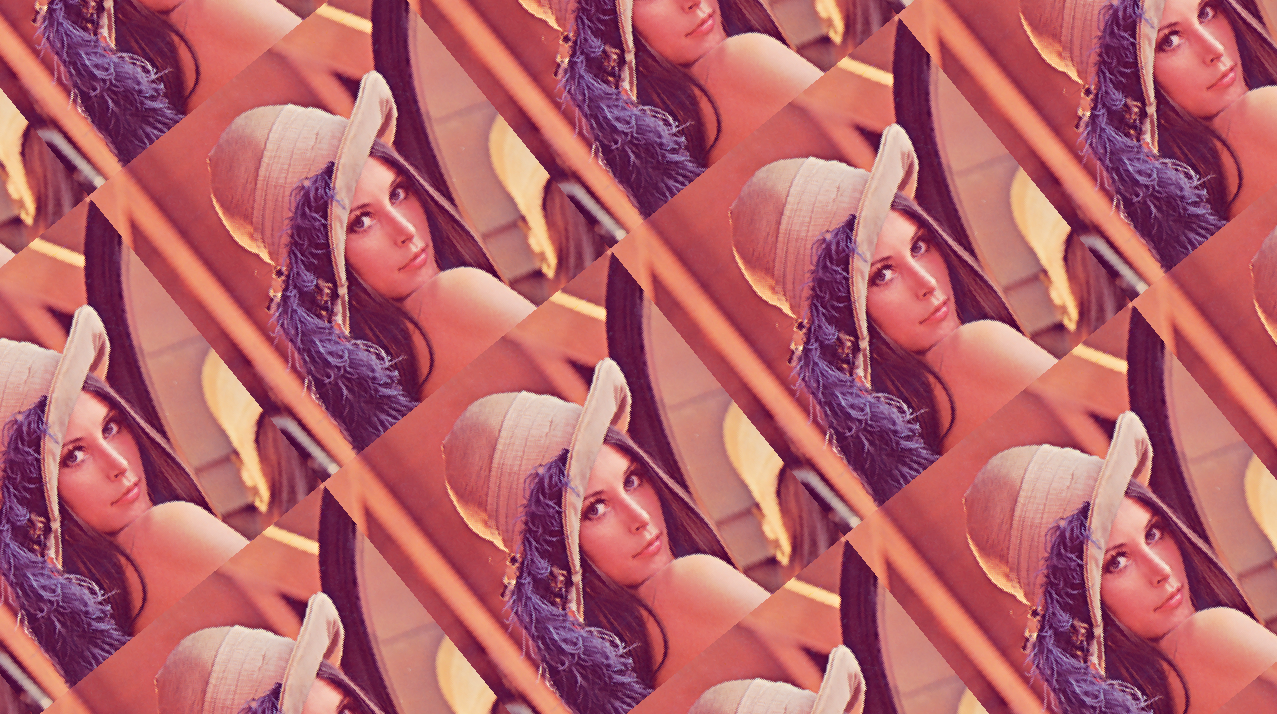
\includegraphics[width=7.5cm]{archivos/rotozoom1}
		\label{fig:rotozoom1}
	\end{subfigure}
	\begin{subfigure}[b]{0.48\textwidth}
		\centering
		
\includegraphics[width=7.5cm]{archivos/rotozoom2}
		\label{fig:rotozoom2}
	\end{subfigure}
	\caption{RotoZoom en distintos estados}
\end{figure}

\section{Deformaciones de imagen}

\subsection{Investigación inicial}

Las deformaciones de imagen son un efecto muy socorrido en el mundo de la \emph{demoscene} y de formas muy distintas. Efectos de lupa y/o deformaciones de lente, estiramientos, efectos de muelle o rebote, torsiones, espirales, en túnel...\\

Sólo implementar todas las diferentes propuestas y efectos de deformaciones de imagen podría llevar su propia investigación y trabajo. No obstante, el denominador común de muchas de estas transformaciones es que usan operaciones trigonométricas, y al final no dejan de ser combinaciones  distintas de senos y cosenos a los que se aplican distintos parámetros.\\

Es por ello que para las deformaciones de imagen, nos centraremos en las deformaciones de onda, pues muchos de los efectos que podemos encontrar en demos parten de estas mismas bases matemáticas.\\

\subsection{Planteamiento formal}

En la figura [\ref{fig:wavefunction}] podemos ver la ecuación de la onda, donde \(A\) es la amplitud de la onda, lo que en nuestra demo se traducirá en la altura máxima y mínima de nuestra onda, en píxeles. \(f\) se corresponde con la frecuencia de la onda (cuántas veces por segundo se completa un ciclo de onda), \(\lambda\) es la longitud de onda (distancia entre dos crestas consecutivas de la onda), \(t\) es el tiempo transcurrido y \(\phi\) es la fase inicial (o desplazamiento inicial con respecto al origen).\\

\begin{figure}[h]
	\centering
	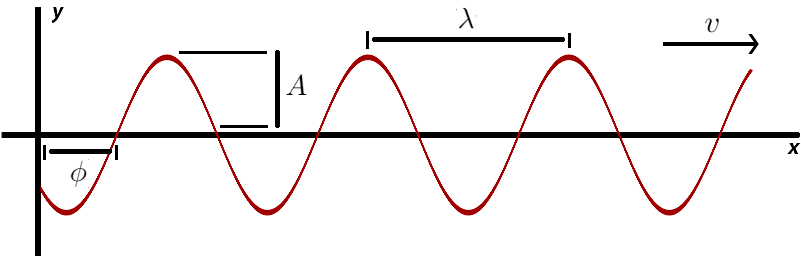
\includegraphics[width=13cm]{archivos/wave}
	\resizebox{6cm}{!}{\(A \sin{(2 \pi v t + \phi)}, v = f \lambda\)}
	\caption{Representación gráfica de la onda y su ecuación}
	\label{fig:wavefunction}
\end{figure}

Además, podemos distinguir dos tipos distintos de onda, dependiendo de su forma de movimiento. Una \textbf{onda transversal} es aquella en la que la dirección de movimiento es perpendicular a la dirección de oscilación\footnote{\url{https://es.wikipedia.org/wiki/Onda_transversal}} mientras que una \textbf{onda longitudinal} es aquella en la que la dirección de movimiento es paralela a la dirección de oscilación\footnote{\url{https://es.wikipedia.org/wiki/Onda_longitudinal}}. Por ejemplo, un muelle es un ejemplo de onda longitudinal, pues oscila (rebota) en la misma dirección en la que se mueve, mientras que las ondas que se producen al lanzar una piedra en el agua son un buen ejemplo de onda transversal (pues mientras que el agua oscila de arriba abajo, la onda avanza en línea recta, perpendicular a su oscilación).\\

En la figura [\ref{fig:transversalwave}] podemos ver la fórmula de la onda transversal. Tiene sentido que el avance de esta onda sea perpendicular a su dirección de oscilación, dado que como se muestra en la figura, el valor de \(y\) depende de \(x\), por lo que el valor en el eje \(y\) depende del valor en el eje perpendicular al mismo. Esto mismo se extrapola a la figura [\ref{fig:longitudinalwave}], dónde el avance de la onda en \(y\) depende de \(y\), por lo que la dirección de propagación coincide con la dirección de oscilación.\\

\begin{figure}[h]
	\centering
	\begin{subfigure}[b]{0.45\textwidth}
		\centering
		\resizebox{4cm}{!}{\(y = A \sin{(2 \pi \frac{x}{\lambda} + \phi)}\)}
		\caption{Onda transversal}
		\label{fig:transversalwave}
	\end{subfigure}
	\begin{subfigure}[b]{0.45\textwidth}
		\centering
		\resizebox{4cm}{!}{\(y = A \sin{(2 \pi \frac{y}{\lambda} + \phi)}\)}
		\caption{Onda longitudinal}
		\label{fig:longitudinalwave}
	\end{subfigure}
\end{figure}

Con todo lo visto, para poder crear nuestra demo de deformaciones de imagen necesitaremos:

\begin{itemize}
	\item Implementar un modo de aplicar deformaciones a nuestra imagen 
	\item Implementar un sistema que permita manejar con facilidad distintas ondas	
	\item Implementar distintos tipos de ondas, con distintos parámetros
\end{itemize}

\subsection{Implementación}

Como podemos ver en el código [\ref{cod:drawdeformation}], empezamos por definir una función delegada que nos devuelva un valor entero en función del valor de entrada, que serán las coordenadas \emph{x} e \emph{y}. De este modo, podemos definir nuestro comportamiento de deformación encapsulado en sus propios métodos, generando un código más fácil de mantener y un programa fácilmente modificable en tiempo de ejecución.\\

\begin{lstlisting}[style=C-color, caption={Dibujado de un pixel aplicando una función que modifica el acceso a textura}, label=cod:drawdeformation]
typedef int (Deformations::*delegate)(int, int);

void Deformations::DrawPixel(int x, int y, float deltaTime, delegate xModifier, delegate yModifier)
{
    int newX = (this->*xModifier)(x, y) % texWidth;
    int newY = (this->*yModifier)(x, y) % texHeight;

    pixels[y * width + x] = texture[newY * texWidth + newX];
}
\end{lstlisting}

Tras ello, definimos diversos métodos que apliquen nuestras funciones de onda, tanto para \emph{x} como para \emph{y}. En el código [\ref{cod:xmodifiers}] podemos ver los modificadores que definimos para \emph{x}. Definimos así un método por defecto que simplemente devuelve la variable sin modificar (por si no queremos aplicar deformación en absoluto o queremos no aplicar transformación en un eje). Tras ello, definimos un método para generar ondas transversales (como podemos ver, la \emph{x} depende de la \emph{y}) y un método para generar ondas longitudinales (donde \emph{x} depende de sí misma). La variable \emph{k} corresponde al número de ondas (\(k = \frac{2 \pi}{\lambda}\)). Además, en nuestro caso sumamos una fase inicial variable, que depende del tiempo (multiplicado por una constante definida por el usuario), de modo que se aplique un desplazamiento incremental a la deformación, generando sensación de movimiento.\\

\begin{lstlisting}[style=C-color, caption={Funciones de deformación en X}, label=cod:xmodifiers]
int Deformations::DefaultXModifier(int x, int y)
{
    return x;
}

int Deformations::TransversalWaveXModifier(int x, int y)
{
    return x + amplitude * sineTable[(y * k + int(accumulatedTime * c)) % mathTableSize];
}

int Deformations::LongitudinalWaveXModifier(int x, int y)
{
    return x + amplitude * sineTable[(x * k + int(accumulatedTime * c)) % mathTableSize];
}

int Deformations::FlagXModifier(int x, int y)
{
    return x + bigAmplitude * sineTable[(y + int(accumulatedTime * c)) % mathTableSize];
}
\end{lstlisting}

Como podemos ver, ahora usamos tablas precalculadas desde el principio, pues ya hemos demostrado en la demo anterior que la única forma de obtener una tasa de fotogramas estable y aceptable es mediante el uso de tablas precalculadas. Calculamos el módulo en función del tamaño de la tabla para asegurarnos de no salirnos de los límites de la misma.\\

Como podemos ver en el código [\ref{cod:xmodifiers}], tenemos un último método al que hemos llamado \emph{FlagModifier}. Esta función ha sido nombrada por el resultado visual que produce, en lugar de haberse elegido su nombre por el tipo de onda que es. Usamos como modificador una onda transversal con una amplitud grande y una longitud de onda también grande (\emph{k} se omite, por lo que \(k = 1\), lo que implica que \(\lambda = 2 \pi\)). Esto produce, al aplicarse sobre la imagen, un efecto similar a una bandera ondeando, de ahí el nombre.\\

Una vez hemos definido nuestras funciones de deformación para \emph{x} e \emph{y}, y habiendo ajustado sus valores, podemos combinarlas y usarlas libremente para crear distintos efectos visuales. Para ello, definimos un vector de pares de modificadores (\lstinline{std::vector<std::pair<delegate, delegate>>}\{. Aunque esta expresión parece algo compleja, es realidad su uso es muy sencillo: al tener un vector de pares de modificadores, podemos añadir fácilmente pares de modificadores y alternarlos. De este modo, podemos aplicar modificadores para \emph{x} e \emph{y} y cambiarlos con facilidad en tiempo de ejecución, aplicando simplemente el siguiente par en el vector.\\

\subsection{Resultado}

Podemos apreciar los resultados de aplicar y combinar las distintas deformaciones en la figura [\ref{fig:alldeformations}].

\begin{figure}
	\centering
	\begin{subfigure}[b]{0.48\textwidth}
		\centering
		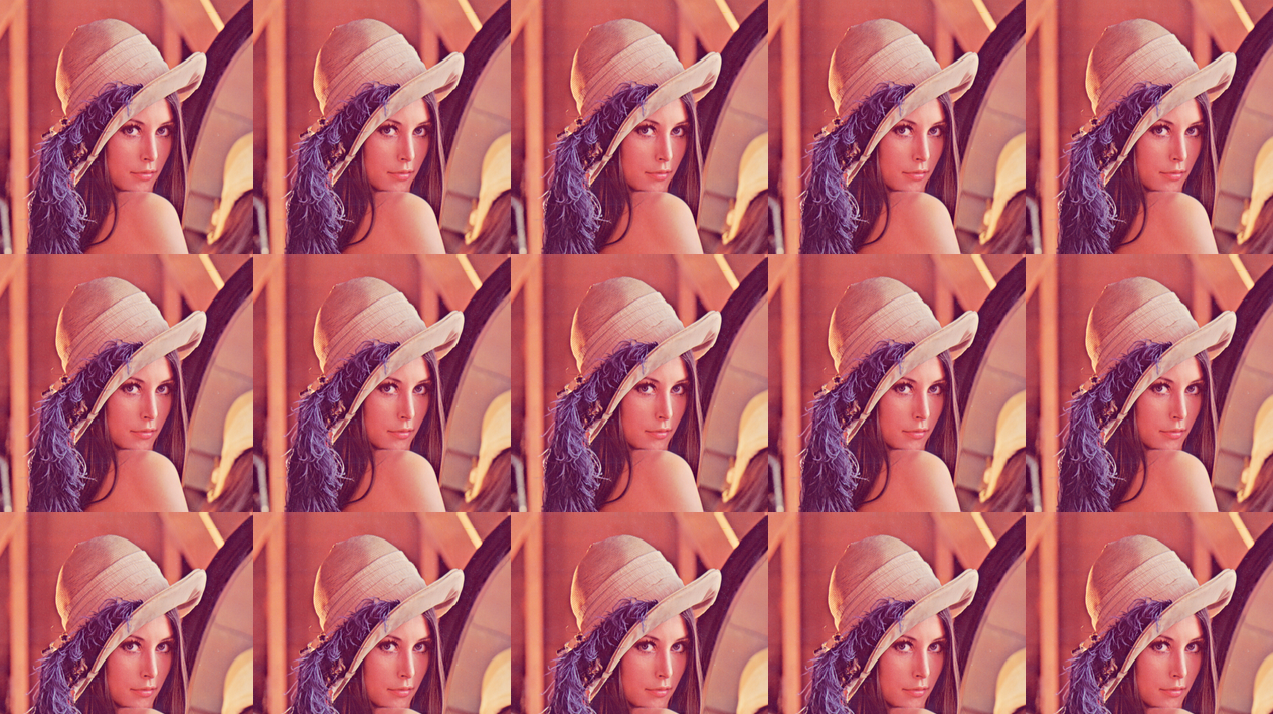
\includegraphics[width=7.5cm]{archivos/deformation1}
		\caption{Sin modificar}
	\end{subfigure}
	\begin{subfigure}[b]{0.48\textwidth}
		\centering
		
\includegraphics[width=7.5cm]{archivos/deformation2}
		\caption{Onda transversal en x}
	\end{subfigure}
\end{figure}
\begin{figure}\ContinuedFloat
	\centering
	\begin{subfigure}[b]{0.48\textwidth}
		\centering
		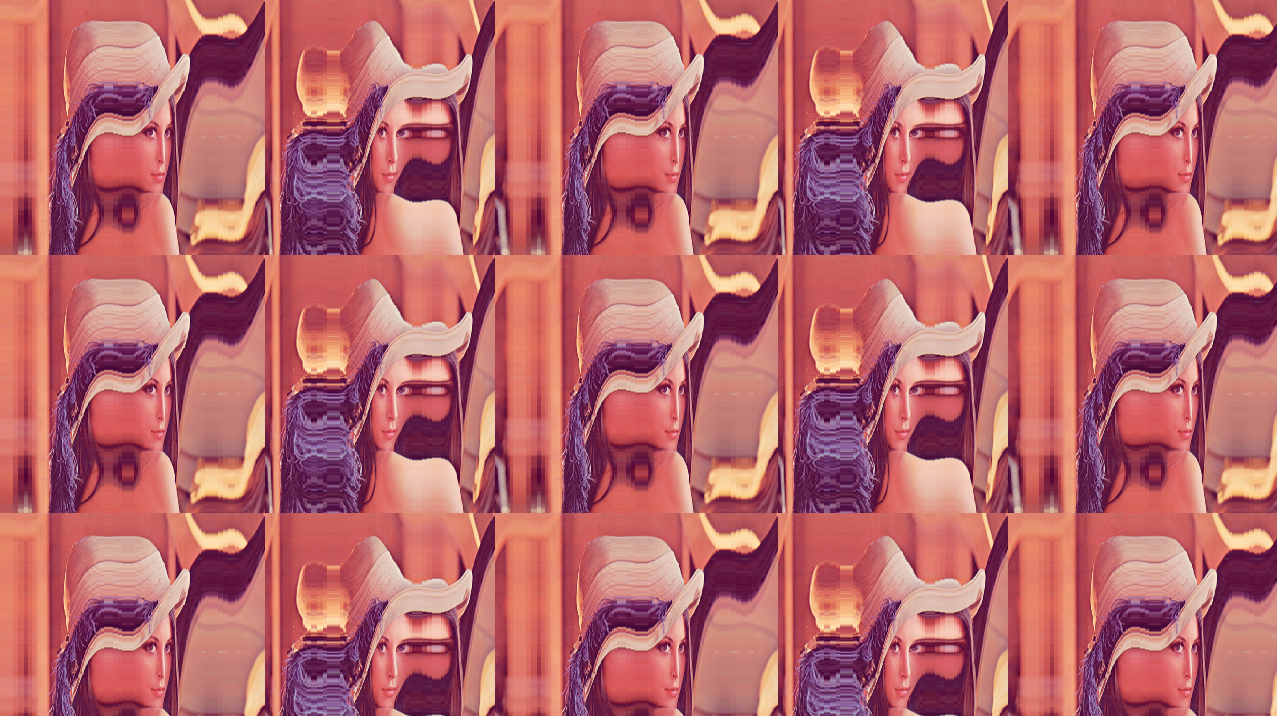
\includegraphics[width=7.5cm]{archivos/deformation3}
		\caption{Onda longitudinal en x}
	\end{subfigure}
	\begin{subfigure}[b]{0.48\textwidth}
		\centering
		
\includegraphics[width=7.5cm]{archivos/deformation4}
		\caption{Transversal en x e y}
	\end{subfigure}
\end{figure}
\begin{figure}\ContinuedFloat
	\centering
	\begin{subfigure}[b]{0.48\textwidth}
		\centering
		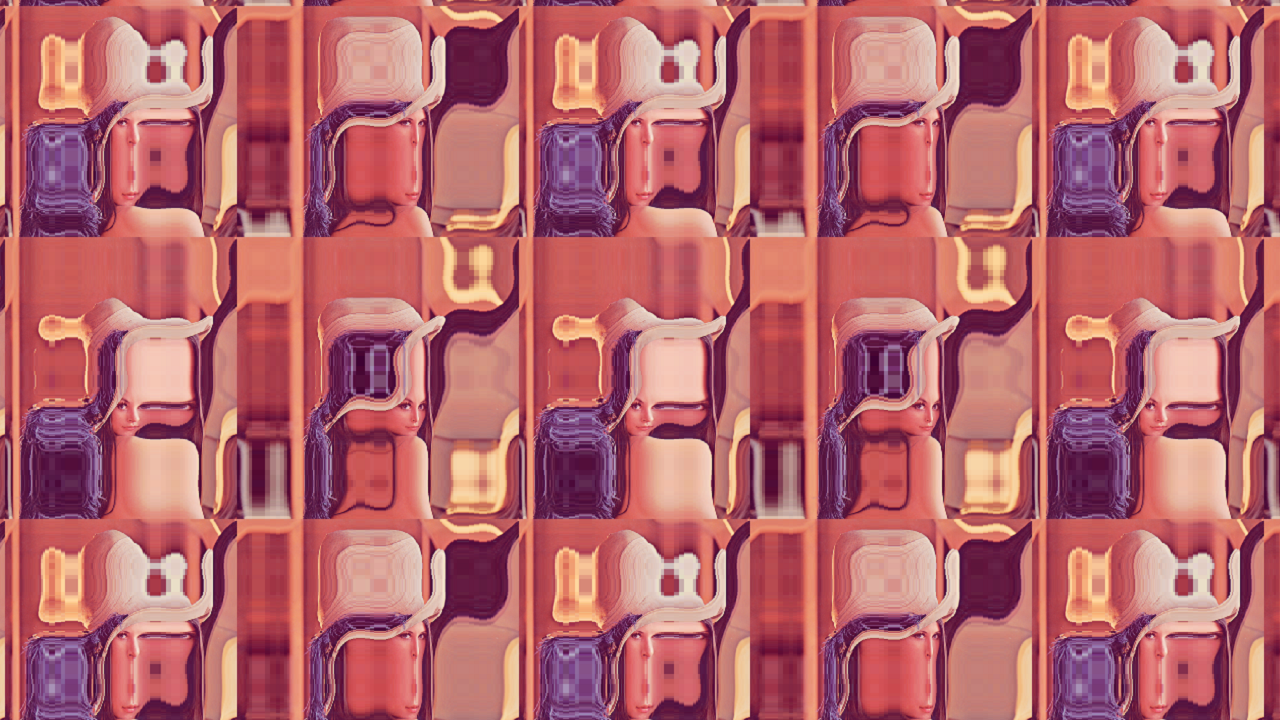
\includegraphics[width=7.5cm]{archivos/deformation5}
		\caption{Mosaico (longitudinal en x e y)}
	\end{subfigure}
	\begin{subfigure}[b]{0.48\textwidth}
		\centering
		\includegraphics[width=7.5cm]{archivos/deformation6}
		\caption{Efecto de bandera}
	\end{subfigure}
	\caption{Distintos efectos de deformación a partir de ondas}
	\label{fig:alldeformations}
\end{figure}

\section{Plasma}

\subsection{Investigación inicial}

El efecto de plasma es otro de los grandes clásicos de la \emph{demoscene}, como el que podemos ver en la figura [\ref{fig:plasma}]. Este efecto existe bien documentado y podemos encontrar múltiples explicaciones y formas de implementarlo.\\

Un tutorial en detalle, muy bien explicado y documentado es el que podemos encontrar en la página de \textbf{Lode's Computer Graphics Tutorial}\footnote{\url{https://lodev.org/cgtutor/plasma.html}}. Este efecto es tan popular que cuenta incluso con su propia página de Wikipedia\footnote{\url{https://en.wikipedia.org/wiki/Plasma_effect}} e incluso en Rosetta Code\footnote{\url{https://rosettacode.org/wiki/Plasma_effect}} podemos encontrar el código para este efecto implementado en más de 20 lenguajes de programación distintos. También podemos encontrar el código para implementar el efecto de Plasma por GPU en Bidouille.org\footnote{\url{https://www.bidouille.org/prog/plasma}}.\\

Como podemos ver, este no es para nada un efecto desconocido o poco documentado, si no que más bien tenemos que, ante tanta información y tantas implementaciones posibles, elegir la que más se adecue al ámbito de este proyecto.

\subsection{Planteamiento formal}

Existen dos principales acercamientos a la implementación del efecto de plasma: combinación de ondas o generación de ruido.\\

Ambos acercamientos son válidos, e incluso se pueden combinar para producir resultados intermedios. El acercamiento por combinación de ondas se basa en la suma o superposición de distintas funciones de onda, con distintas frecuencias, longitudes de onda y amplitudes, asignando color en función del resultado de la combinación. El acercamiento por generación de ruido se basa, por otro lado, en la generación de un ruido que tenga coherencia local, como por ejemplo el ruido Perlin\footnote{\url{https://en.wikipedia.org/wiki/Perlin_noise}}.\\

Los resultados de generación de ruido mediante Perlin u otros algoritmos de generación de ruido (fractal, simplex...), no obstante, suelen dar resultados más similares a nubes o turbulencias que a plasma, y suelen requerir de niveles bajos de detalle (pocas iteraciones, si se trata de un algoritmo iterativo) o de suavizados posteriores (calculando valores medios o con efectos de desenfoque) para ser suficientemente convincentes. Además de esto, a la hora de animarlos, el movimiento no resulta tan natural como en el uso de ondas, dado que aunque el ruido tenga coherencia local, sigue existiendo un factor de aleatoriedad que puede romper la coherencia del movimiento.\\

Es por ello que se opta por implementar un efecto de plasma mediante la combinación de ondas. Estos serán los pasos a seguir:

\begin{itemize}
	\item Hallar una combinación de ondas que produzca el efecto deseado
	\item Aplicar un degradado de color dado el resultado de la combinación
\end{itemize}

\subsection{Implementación}

En el código [\ref{cod:multiwave}] se muestra una versión simplificada del código para generar ondas, de modo que sea más fácil de leer (dado que el código real emplea tablas precalculadas y guarda cada operación que se repite más de una vez en variables temporales).\\

\begin{lstlisting}[style=C-color, caption={Combinación de distintas ondas}, label=cod:multiwave, escapechar=|]
value += sin((j * i) / (j + i + 1) * scale + accumulatedTime * 191);|\label{line:plasma1}|
value += sin(((width - i) * j) / ((width - i) + j + 1)* scale + accumulatedTime * 157);|\label{line:plasma2}|
value += sin((i * (height - j)) / (i + (height - j) + 1) * scale + accumulatedTime * 113);|\label{line:plasma3}|
value += sin(((width - i) * (height - j)) / ((width - i) + (height - j) + 1) * scale + accumulatedTime * 67);|\label{line:plasma4}|
\end{lstlisting}

Podemos comparar este código con el resultado de la figura [\ref{fig:allwaves}], donde se muestra el resultado que genera cada línea de código, la onda en que resulta de forma separada.\\

\begin{figure}[h]
	\centering
	\begin{subfigure}[b]{0.45\textwidth}
		\centering
		\includegraphics[width=6cm]{archivos/plasma1}
		\caption{Línea [\ref{line:plasma1}]}
	\end{subfigure}
	\begin{subfigure}[b]{0.45\textwidth}
		\centering
		\includegraphics[width=6cm]{archivos/plasma2}
		\caption{Línea [\ref{line:plasma2}]}
	\end{subfigure}
	\begin{subfigure}[b]{0.45\textwidth}
		\centering
		\includegraphics[width=6cm]{archivos/plasma4}
		\caption{Línea [\ref{line:plasma3}]}
	\end{subfigure}
	\begin{subfigure}[b]{0.45\textwidth}
		\centering
		\includegraphics[width=6cm]{archivos/plasma3}
		\caption{Línea [\ref{line:plasma4}]}
	\end{subfigure}
	\caption{Cada una de las ondas que son sumadas (con su correspondencia a línea de código)}
	\label{fig:allwaves}
\end{figure}

Si nos fijamos en el código y en las imágenes, podemos ver que todo lo que hacemos es crear cuatro ondas, yendo cada una hacia una de las esquinas de la pantalla y que están desfasadas entre ellas. Los números elegidos para la fase no son aleatorios, pues todos ellos son números primos. Esto es importante, pues si la fase de alguna onda es múltiplo de otra, se pueden producir formas forzadas o bucles que rompan con la sensación de aleatoriedad y continuidad, dado que su desfase es proporcional. Es por ello que el mejor modo de asegurar que no se produzcan estos \emph{acoples} entre las ondas es multiplicando la fase por números primos, de modo que las fases de las ondas no tengan múltiplos comunes y por tanto no puedan acoplarse o dar sensación de periodicidad.\\  

Una vez hemos sumado nuestras ondas, dividimos entre 4 para normalizar el resultado (entre -1 y 1) y a continuación convertimos este intervalo en un valor entero que oscile entre 0 y 255. De este modo obtenemos un índice con el que acceder a un color específico dentro del degradado de colores que hayamos definido previamente.\\

El resultado de esta combinación de ondas resulta en un efecto bastante convincente, como podemos ver en la figura [\ref{fig:whiteplasma}].\\

\begin{figure}[h]
	\centering
	\includegraphics[width=8cm]{archivos/whiteplasma}
	\caption{Efecto de plasma}
	\label{fig:whiteplasma}
\end{figure}

Ahora tan sólo nos queda añadir la capacidad de cambiar de degradado de color, como hemos hecho ya en otras demos, para conseguir así un resultado más convincente o visualmente impactante.

\subsection{Resultado}

\begin{figure}[h]
	\centering
	\begin{subfigure}[b]{0.48\textwidth}
		\centering
		\includegraphics[width=7.5cm]{archivos/redplasma}
		\caption{Efecto lámpara de lava}
	\end{subfigure}
	\begin{subfigure}[b]{0.48\textwidth}
		\centering
		\includegraphics[width=7.5cm]{archivos/greenplasma}
		\caption{Efecto eléctrico}
	\end{subfigure}
\end{figure}

\section{Planos infinitos}

\subsection{Investigación inicial}

El efecto de planos infinitos es muy conocido en la \emph{demoscene}, pero es especialmente popular y conocido en el mundo del videojuego, donde fue popularizado por Nintendo como el famoso Modo 7 \footnote{\url{https://en.wikipedia.org/wiki/Mode_7}} que incluía la SNES. Este era un modo gráfico de esta consola que permitía realizar transformaciones afines, mediante las que se lograba el efecto de planos infinitos.\\

Este efecto básicamente consistía el uso de una textura bidimensional que se transformaba para dar efecto de profundidad o tridimensionalidad, como podemos ver en la figura [\ref{fig:mode7}].\\

\begin{figure}[h]
	\centering
	\includegraphics[width=8cm]{archivos/mode7}
	\caption{Modo 7 (efecto de planos infinitos) en la SNES - Fuente: \href{https://en.wikipedia.org/wiki/Mode_7\#/media/File:Mode_7_Test-0000.png}{Wikipedia (por Anomie)}}
	\label{fig:mode7}
\end{figure}

Gracias a este efecto fueron posibles juegos como el primer \emph{Mario Kart}\footnote{\url{https://en.wikipedia.org/wiki/Super_Mario_Kart}}, donde la pista o el circuito no eran más que una textura 2D de grandes dimensiones transformada, para que pareciera un plano o un circuito 3D.\\

Este efecto está muy bien documentado y se puede encontrar su explicación formal tanto en Wikipedia como numerosos tutoriales que ofrecen distintos acercamientos, como este tutorial de \emph{One Lone Coder}\footnote{\url{https://www.youtube.com/watch?v=ybLZyY655iY&t=646s}} en que ofrece una explicación formal y da su propio planteamiento para implementar este modo o este otro tutorial en Coranac.com\footnote{\url{https://www.coranac.com/tonc/text/mode7.htm}} dónde se nos ofrecen tres implementaciones distintas, con distintos acercamientos, y se hace una reflexión sobre los resultados obtenidos.

\subsection{Planteamiento formal}

El efecto de planos infinitos está muy bien documentado, bajo distintos acercamientos, uno de los cuales es el Modo 7, aunque también existen otras formas de causar un efecto similar.\\

Siguiendo el espíritu de este trabajo, intentaremos implementar el efecto de planos infinitos sin usar código de referencia, simplemente usando el material visual disponible para intentar deducir cómo podríamos implementar este efecto. En la figura [\ref{fig:planes}], de creación propia, vemos un posible acercamiento a este efecto, que es el que seguiremos e intentaremos implementar.\\

\begin{figure}[h]
	\centering
	\includegraphics[width=12cm]{archivos/planes}
	\caption{Nuestro acercamiento a los planos infinitos}
	\label{fig:planes}
\end{figure}

En esta figura [\ref{fig:planes}], el cuadro negro representa la pantalla o la parte visible de la textura, la línea roja representa la línea del horizonte, punto a partir del cual no se muestra nuestra textura en pantalla.\\

Para facilitar la visualización del contenido, la parte de la textura fuera de pantalla se ha oscurecido y la parte de la textura en pantalla pero tras la linea del horizonte se ha aclarado, de modo que la porción visible destaque. Además, se ha rellanado el espacio en de pantalla adyacente a nuestra textura con un verde más oscuro, para completar la imagen y facilitar su visualización.\\

Como vemos, partimos de una textura bidimensional, plana. A continuación, estiramos la textura en su parte baja y la apretamos en la parte alta. Dicho de un mejor modo: hacemos nuestra textura depender de la altura, de modo que a mayor altura, más se estreche y viceversa. Ya solo con esto, nuestra imagen gana sensación de profundidad y tridimensionalidad. Pero además, queremos ser capaces de moverla. Para ello, una vez que nuestra textura ha sido convenientemente deformada, rotamos la imagen usando la fórmula mostrada en la figura [\ref{fig:transform}].\\

Una vez que nuestra textura ha sido deformada y rotada como queremos, podemos desplazarla, de modo que así, es pantalla, dará sensación de movimiento y avance. Realmente, todo lo que hacemos es aplicarle las transformaciones 2D que ya vimos con el RotoZoom pero con un contexto y un fin distintos.

\subsection{Implementación}

\begin{lstlisting}[style=C-color, caption={Código para generar un efecto básico de planos infinitos, con escalado, rotación y translación}, label=cod:infiniteplanes, escapechar=|]
for (int j = 0, nh = height / 2; j < nh; j++)
{
    for (int i = -width / 2, nw = width / 2; i < nw; i++)
    {
        Point2D projectedPoint(i / (float)j, fieldOfView / (float)j);
        projectedPoint *= textureScale;
        
        Point2D rotatedPoint(projectedPoint.X * cosine - projectedPoint.Y * sine,
                                projectedPoint.X * sine + projectedPoint.Y * cosine);
                             
        Pixel colour = texture[Fast::Abs((int(rotatedPoint.Y + cameraPosition.Y) % texHeight) * texWidth +
                                            int(rotatedPoint.X + cameraPosition.X) % texWidth)];
                                         
        pixels[(j + nh) * width + (i + nw)] = colour;|\label{line:planesaccess}|
    }
}
\end{lstlisting}

Como podemos ver en el código, recorremos media pantalla en altura, desde 0 hasta la mitad de la pantalla, y desde \(-x \div 2\) hasta \(+x \div 2\), recorriendo así toda la anchura de la pantalla. Esta decisión no es aleatoria, pues como vemos más adelante, en la línea [\ref{line:planesaccess} sumamos la mitad de la altura y la anchura, desplazando las coordenadas \emph{i} y \emph{j}. Hacemos esto por conveniencia, pues nos facilita los cálculos, ya que para transformar nuestra textura lo hacemos con respecto al origen de la pantalla (el \emph{(0, 0)} equivale a la esquina superior izquierda) y luego desplazamos el resultado obtenido, como podemos ver en la figura [\ref{fig:desplazamiento}. Recordemos que el orden de las transformaciones no es conmutativo, por lo que primero debemos escalar y rotar con respecto al origen, dejando el desplazamiento como el último paso. De lo contrario, obtendríamos resultados incoherentes.\\

\begin{figure}[h]
	\centering
	\includegraphics[width=8cm]{archivos/desplazamiento}
	\caption{Posición relativa de la textura antes y después de ser transformada}
	\label{fig:desplazamiento}
\end{figure}

Con esta forma de recorrer nuestra textura, nos aseguramos de operar con respecto al origen, y trasladamos los resultados obtenidos posteriormente.\\

Dentro del bucle, empezamos por la primera transformación (equivalente a estirar la textura en la parte inferior y estrechar en la superior). Para obtener este efecto, basta con dividir 

\subsection{Refinamiento}

\begin{itemize}
	\item \textbf{Opacidad}
	\item \textbf{Relieve}
\end{itemize}

\subsection{Resultado}

rgerg
sgsdgsfdh

sg

drga

rg

ergregearg

rgerg


\section{Geometría}


\subsection{Investigación inicial}

rgerg
sgsdgsfdh

sg

drga

rg

ergregearg

rgerg

\subsection{Planteamiento formal}

rgerg
sgsdgsfdh

sg

drga

rg

ergregearg

rgerg

\subsection{Implementación}

rgerg
sgsdgsfdh

sg

drga

rg

ergregearg

rgerg

\subsection{Refinamiento}

rgerg
sgsdgsfdh

sg

drga

rg

ergregearg

rgerg

\subsection{Resultado}

rgerg
sgsdgsfdh

sg

drga

rg

ergregearg

rgerg

\chapter{Demo final}

\section{Introducción}

Hasta ahora hemos estado revisando algunos de los efectos gráficos más conocidos y comunes en el mundo de la \emph{demoscene}, analizándolos desde el punto de vista más analítico posible pero también intentando comprender su esencia y trasfondo.\\

Los efectos gráficos son el pilar, la base, que construye el mundo de la \emph{demoscene}, pero un solo efecto no hace una demo, pues una demo consiste en un conjunto de efectos gráficos compilados en un solo ejecutable, normalmente acompañados además de música que se reproduce de forma sincronizada.\\

Tras haber estudiado todos los efectos expuestos anteriormente, llega el momento de utilizar el conocimiento adquirido para intentar generar un obra, una \textbf{demo}, lo más interesante posible. Para ello, será necesario no sólo aplicar lo aprendido, si no también saber hacerlo de una forma que tenga una cierta coherencia en conjunto, de modo que resulte visualmente agradable. No hemos de olvidar que al fin y al cabo la \emph{demoscene} es tanto una práctica de ingeniería como de arte.\\

Si bien en este trabajo para nada se aspira a lograr una obra de arte, sí que se perseguirá un cierto sentido estético a lo largo de la composición, de forma que la compilación de todas las demos anteriores resulte lo más coherente y orgánica posible.\\

Como referencias a esta demo se pueden tomar todas aquellas que se han citado y mostrado previamente, pues esta demo pretende ser un humilde tributo y una humilde revisión de la cultura de la \emph{demoscene}, yendo a sus orígenes y efectos más clásicos y trayéndolos de vuelta a los computadores de hoy en día, ejecutando únicamente por CPU y en tiempo real.\\

\section{Planteamiento inicial}

Para desarrollar esta demo hay varias limitaciones o retos de base que nos debemos plantear. En primer lugar, la música juega un factor clave en las demos, y sin embargo hasta ahora no tenemos ningún mecanismo para generar sonido.\\

Además, la demo se ejecutará exclusivamente en la CPU del ordenador, lo cual si bien resulta muy interesante, dado que pone en valor las capacidades de cómputo de un ordenador, también resulta un factor limitante, pues la manipulación de millones de píxeles por segundo no es una tarea trivial, y aún menos si hay operaciones matemáticas complejas de por medio. Es por ello que deberemos aplicar todo lo aprendido para tratar de optimizar y estirar el rendimiento al máximo, y cuando esto no sea posible, buscar otras opciones o caminos que enmascaren las limitaciones técnicas de la máquina.\\

Por otro lado, los efectos gráficos que hemos mostrado hasta ahora son tan sólo muestras simplificadas de modo que resulten lo más explícitas y entendibles posible, pero ahora es el momento de buscar resultados más complejos o interesantes a partir de la base que ya ha sido planteada.\\

Por último, los efectos gráficos creados hasta el momento son bastante distintos o inconexos entre sí, por lo que será importante encontrar un modo orgánico de generar transiciones entre los mismos o combinarlos de una forma coherente.\\

A grandes rasgos, estas son las tareas necesarias para elaborar nuestra demo final:

\begin{itemize}
	\item Permitir la generación de sonido o música
	\item Aplicar o combinar todos y cada uno de los efectos gráficos explicados anteriormente
	\item Aplicar música a la demo coordinada con los efectos gráficos
\end{itemize}

\section{Generar sonido}

Antes de saltar a la implementación, conviene explicar muy brevemente como se representa el sonido de forma digital. Se asume, no obstante, que se conoce de forma básica el funcionamiento del sonido (física de ondas) y su representación matemática. Como ya sabemos, el sonido no es más que una vibración, una oscilación y por tanto, un movimiento ondulatorio. Si se requiere de un breve repaso sobre el funcionamiento de una onda, se puede encontrar en el planteamiento formal del efecto de deformaciones de imagen [\ref{sec:deformaciones}]\\

\begin{figure}[h]
	\centering
	\includegraphics[width=13cm]{archivos/soundWave}
	\caption{Onda sinusoidal y su discretización}
	\label{fig:soundWave}
\end{figure}

Como podemos ver en la figura [\ref{fig:soundWave}], un sonido se puede representar como una onda (o una combinación de ondas). En el dominio analógico (en rojo), una onda es continua, sin embargo, en el dominio digital (en azul) solo se puede representar una cantidad discreta de valores de la onda, con la consiguiente pérdida de precisión. Es por ello, que para almacenar una onda en el dominio digital definimos una frecuencia de muestreo (equivalente a las líneas verticales de la imagen) y un formato o resolución de muestra (equivalente a las líneas horizontal en la imagen) de modo que cualquier valor intermedio, que no pueda ser representado, será aproximado al valor más cercano.\\

Habiendo dejado esto claro, pasamos a intentar generar sonido por computador. Siguiendo con la dinámica general de este trabajo, la generación de sonido debería ser, en la medida de lo razonable, gestionada por nosotros. La idea inicial es la de usar una librería de sonido para la música del mismo modo que usamos OpenGL para los gráficos, es decir, usar una librería que actúe simplemente como envoltorio y nos genere una capa de abstracción con respecto al sistema operativo, pero una vez hecho esto, generar el sonido desde cero.\\

Tras una breve investigación, las dos opciones más factibles parecían OpenAL\footnote{\url{https://www.openal.org}} y PortAudio\footnote{\url{http://www.portaudio.com}}. Si bien OpenAL es el equivalente directo de OpenGL pero para audio, PortAudio acabó siendo la librería elegida. OpenAL es una librería más estandarizada y potente, que permite generar sonido en 3D y tiene un modo de funcionamiento similar al de su casi homónimo OpenGL. Pero esta potencia viene al coste de una mayor complejidad de uso. PortAudio, en cambio, siendo una librería también de código abierto y multiplataforma, se centra en la simplicidad. Y por ello mismo se optó por ella, ya que parecía innecesario tener que aprender a manejar toda una librería potente y completa con el mero objetivo de usarla como una abstracción de cara al sistema operativo.\\

Una vez tenemos la librería elegida, llega el momento de empezar a implementar nuestro sistema capaz de generar sonido. Todo lo que PortAudio necesita para empezar a funcionar es inicializar la librería y crear un flujo (\emph{stream}) de sonido, al que se le pasa una función delegada controlada por el usuario.\\

\begin{lstlisting}[style=C-color, caption={Código necesario para inicializar PortAudio},label=cod:initialisePortAudio]
Pa_Initialize();
Pa_OpenDefaultStream(&stream, INPUT_CHANNELS, OUTPUT_CHANNELS, paFloat32, SAMPLE_RATE, FRAMES_PER_BUFFER, AudioCallback, 0);
Pa_StartStream(stream);
\end{lstlisting}

Para entender no obstante, cómo funciona PortAudio y los parámetros que nos pide, debemos entender cómo funciona el audio por computador. Como podemos ver en el código [\ref{cod:initialisePortAudio}], una vez inicializamos la librería, abrimos un flujo de sonido. Para hacer esto, no obstante, debemos pasar una serie de parámetros significativos. El primero de ellos, \emph{stream}, se trata simplemente de una estructura del tipo \emph{PaStream}. Esto es un tipo definido por los creadores de la librería y del que realmente no tendremos que preocuparnos, pues es gestionado internamente y no tendremos que realizar ningún tipo de operación con el mismo. La función principal de este tipo es la gestión de distintos canales de entrada y salida de sonido. A continuación debemos indicar los canales de entrada y de salida. Un canal de entrada se corresponde con una fuente de entrada de sonido. Aunque un canal no se corresponde necesariamente a un dispositivo, normalmente un canal de entrada se corresponde con un único dispositivo de grabación. Si en nuestra demo necesitásemos grabar audio, necesitaríamos entonces al menos un canal de entrada. Un canal de salida se corresponde normalmente, aunque no de forma necesaria, con un solo dispositivo de reproducción de audio, o en otras palabras, con un altavoz. Como en nuestra demo no necesitaremos grabar audio pero sí queremos reproducir audio estéreo, necesitaremos pues definir dos canales de salida.\\

Como nota, puntualizar que como se ha dicho anteriormente, un canal de entrada o salida no se corresponde necesariamente con un dispositivo físico. Esto es porque podemos por ejemplo definir dos canales de entrada que se correspondan con un único dispositivo de grabación, y sin embargo, dar a cada entrada de audio un tratamiento distinto. Por ejemplo, usar la entrada de un canal para generar eco y la del otro para generar distorsión, para posteriormente combinar los dos canales de entrada en un único canal de salida que tenga ambos efectos combinados. Del mismo modo, también es posible redirigir más de un canal al mismo dispositivo de reproducción. Por tanto, no existe una correspondencia directa entra canal y dispositivo, si bien es cierto que en muchos casos la suele haber.\\

Volviendo al código en [\ref{cod:initialisePortAudio}], una vez hemos definido que queremos dos canales de salida, llega el momento de definir el formato de muestra. Esto es, definir qué formato tendrá una única muestra de sonido. El valor de una muestra representa el valor de la amplitud del sonido en un instante dado. El sonido de los primeros ordenadores, el tan conocido como \emph{música de 8 bits}, tenía un formato de 8 bits interpretados como un entero por muestra. Esto quiere decir que la unidad mínima de sonido reproducible ocupaba 8 bits, y por tanto podía tener 256 valores distintos para la amplitud, que, para tratarse de sonido, podemos apreciar que es una resolución muy baja. De ahí que la música de 8 bits sonase robótica y poco orgánica, entre otras causas. De hecho, la música en 8 bits tan solo permitía 128 valores distintos, si tenemos en cuenta que en una onda que oscila en el origen, la mitad de los valores están por encima del cero y la otra mitad por debajo, por lo que de forma efectiva, contamos con 128 valores y su equivalente negativo. La música en 16 bits, que fue el siguiente paso, ya permitía definir más de 64000 valores distintos para la amplitud. Si escuchamos de hecho la diferencia entre la música de 16 bits y la música de 8 bits, se denota un cambio significativo. El formato que nosotros definimos en nuestra demo, no obstante, es el de un número en coma flotante de 32 bits. Nuestra amplitud máxima será 1 y nuestra amplitud mínima del sonido generado será -1. No obstante, como trataremos con números decimales, dispondremos de una gran resolución.\\

A continuación, una vez definido el formato de muestra (cuántos bits por muestra y cómo se deben interpretar -entero, coma fija, coma flotante...-) definimos el ratio de muestra, comúnmente denominado como la \emph{frecuencia de muestreo}, o en otras palabras, cuántas muestras queremos por segundo. Tal y como indica el teorema del muestro de Nyquist\footnote{\url{https://es.wikipedia.org/wiki/Teorema_de_muestreo_de_Nyquist-Shannon}}, para generar un sonido a una frecuencia determinada, necesitamos al menos el doble de muestras por segundo que la frecuencia que se pretende muestrear. De media, el ser humano es capaz de percibir frecuencias de entre 20 y 20000 Hercios, de modo que si queremos tener la habilidad de generar cualquier frecuencia audible, necesitaremos al menos 400000 muestras por segundo. En nuestra demo definimos una frecuencia de muestreo de 44100 muestras por segundo. El motivo de la elección de este número se debe a motivos históricos, ya que era la frecuencia de muestreo de los CD, ligeramente superior al espectro de sonido audible por cuestiones de formato y conveniencia\footnote{\url{https://es.wikipedia.org/wiki/Frecuencia_de_muestreo}}.\\

A continuación debemos definir la cantidad de muestras por \emph{buffer}. Como acabamos de explicar, para reproducir un sonido en cualquier frecuencia audible, es necesario contar con al menos 40000 muestras por segundo, y en nuestro caso definimos 44100 muestras de sonido por segundo. Pasar estas muestras una a una sería extremadamente poco eficiente, por no decir imposible. La tarjeta de sonido es la encargada de generar y reproducir audio, de modo que cada vez que reproducimos audio, la CPU debe comunicarse con la tarjeta de sonido. 40000 accesos por segundo a la tarjeta de sonido para enviar un solo dato es una locura, y muy lento. Es por ello que se define un \emph{buffer}. Cuando la CPU le pasa datos a la tarjeta de sonido, no lo hace de uno en uno, si no que manda la información en bloques de datos, reduciendo así la cantidad de comunicaciones con la tarjeta de sonido, que son operaciones bloqueantes. Con este parámetro, podemos definir el tamaño de los bloques de datos que se le pasan a la tarjeta de sonido. Bloques muy pequeños implican muchos accesos a la tarjeta de sonido, bloques muy grandes implican una gran cantidad de datos que transferir y una tasa de actualización muy baja (dado que nuestra función delegada se encarga de generar un bloque de datos por llamada, contando con la información en el momento de llamada, por lo que si esta información se actualiza a mitad de la generación de un bloque, la actualización no se verá reflejada hasta la siguiente llamada a nuestra función). Por tanto, conviene elegir un tamaño de \emph{buffer} que resulte razonable, ni demasiado pequeño, ni excesivo. En nuestra demo definimos un tamaño de 256 muestras por \emph{buffer}, lo que se traduce en unos 170 accesos a la tarjeta de sonido por segundo, y unas 170 llamadas a nuestra función delegada por segundo. Del mismo modo, el tamaño de cada \emph{buffer} será de 2KB (4 bytes -32 bits- por muestra, dos canales, 256 muestras por  canal por \emph{buffer}), un tamaño que no resulta trivial pero que es muy pequeño.\\

Tras ello, los siguientes dos parámetros que hemos de pasar son una función delegada a la que PortAudio llamará de forma interna para generar sonido y, de forma opcional, una estructura definida por el usuario. En nuestro caso, realizaremos todas las operaciones necesarias desde la función delegada, y tenemos todos los datos que necesitamos en nuestra clase. Podremos acceder a estos datos desde nuestra función delegada, ya que es un miembro estático de nuestra clase para reproducir audio. Por tanto, pasaremos un 0 (también sería posible y equivalente en este caso pasar un \emph{nullptr}) para indicar que no haremos uso de ninguna estructura de datos definida por el usuario.\\

Llega ahora el momento de echar un vistazo a la función delegada que puede ser definida por el usuario:\\

\begin{lstlisting}[style=C-color, caption={Función delegada que pasamos a PortAudio},label=cod:audioCallback, escapechar=|]
int Imp_Audio::AudioCallback(const void *inputBuffer, void *outputBuffer,
                             unsigned long framesPerBuffer,
                             const PaStreamCallbackTimeInfo *timeInfo,
                             PaStreamCallbackFlags statusFlags,
                             void *userData)
{
    float *out = (float *)outputBuffer;
    static long int currentCount = 0;

    for (unsigned long i = 0; i < framesPerBuffer; i++)
    {
        currentCount++;

        Imp_Audio::UpdateNotes(currentCount);

        *out++ = Imp_Audio::GetLeftValue();  /* left */ | \label{line:left}|
        *out++ = Imp_Audio::GetRightValue(); /* rigth */| \label{line:right}|
    }
    return 0;
}
\end{lstlisting}

Aunque la cantidad de parámetros que recibe la función delegada puede abrumar a primera vista, la realidad es que apenas usamos unos pocos, como podemos ver en el código [\ref{cod:audioCallback}].\\

No usamos el \emph{inputBuffer}, dado que no hemos definido ningún canal de entrada, del mismo modo que tampoco usamos las variables \emph{timeInfo}, \emph{statusFlags} o \emph{userData}, las dos primeras porque son variables que nos aportan información extra pero que no nos resultan especialmente relevantes y la última porque es el argumento que se corresponde con la estructura de datos definida por el usuario que en nuestro caso hemos decidido no definir. Por tanto, sólo estamos interesados en dos variables, el \emph{outputBuffer}, que se corresponde con el \emph{buffer} para la salida de datos, es decir, es el \emph{buffer} cuyos datos son pasados a la tarjeta de sonido para ser reproducidos por el ordenador y por otro lado, la variable \emph{framesPerBuffer}, que recordemos que habíamos definido previamente con el valor 256 y que nos indica por cada llamada a la función, cuántas muestras por canal debemos incluir en el \emph{buffer}. Si nos fijamos en las líneas [\ref{line:left}] y [\ref{line:right}], veremos que en estas líneas asignamos un valor a la posición actual del \emph{buffer} y a continuación la incrementamos. Como podemos recordar, hemos definido dos canales de salida de audio, dado que queremos audio estéreo. Esto implica, por tanto, que nuestro \emph{buffer} deberá ser rellenado con muestras para ambos canales. Estas muestras se leen de forma intercalada, de modo que si visualizamos nuestro \emph{buffer} como un \emph{array}, su primer valor se corresponderá con la primera muestra del canal izquierdo, su segundo valor con la primera muestra del canal derecho, su tercer valor con la segunda muestra del canal izquierdo, y así sucesivamente... Esto nos permite, de forma bastante sencilla, asignar valores a nuestros canales de salida de audio.\\

Antes de continuar ahondando en el funcionamiento del sistema de sonido, vale la pena explicar su funcionamiento de forma genérica, a partir de lo previamente construido.\\

En nuestro sistema, tenemos un vector estático de notas. Podemos ver la estructura de una nota en la figura [\ref{fig:note}]. Por cada muestra que añadimos al \emph{buffer} de salida, actualizamos los valores de todas las notas que se están reproduciendo actualmente, basándonos en la variable entera \emph{currentCount}, que se actualiza por iteración. De esta modo, usamos \emph{currentCount} para actualizar el valor de nuestras notas de forma muy similar a como usamos el valor de \emph{deltaTime} para actualizar nuestras demos. De hecho, ambas variables tienen una relación directa con el tiempo, ya que \emph{deltaTime} representa el tiempo transcurrido desde el fotograma anterior mientras que \emph{currentCount} representa el número de muestra que se está actualizando, y como sabemos, actualizamos 44100 muestras por segundo, por lo que cada 44100 actualizaciones de este valor, habrá transcurrido un segundo.\\

Una vez actualizamos el valor de nuestras notas, llega el momento de asignarlas a la salida. Para ello, llamamos a dos funciones que respectivamente nos devolverán el valor para la salida de audio izquierda y el valor para la salida de audio derecha, basándose en la posición de las notas que se están reproduciendo actualmente.\\ 

%@startuml
%
%class Note << (S,#FF7700) Struct >>
%{
%  +float (*generateWave)(frequency, count)
%  +Envelope envelope
%  +float frequency
%  +float volume
%  +float position
%  +float lifetime
%  +float currentEnvelopeValue
%  +float resultingSound
%}
%
%class Envelope << (S,#FF7700) Struct >>
%{
%  +float attack
%  +float decay
%  +float sustain
%  +float release
%  +float peakAmplitude
%  +float sustainAmplitude
%  
%}
%
%hide empty members
%
%@enduml

\begin{figure}[h]
	\centering
	\includegraphics[width=13cm]{archivos/note}
	\caption{Estructura de una nota y su envolvente}
	\label{fig:note}
\end{figure}

Una vez que entendemos de forma simplificada como funciona nuestro sistema, llega el momento de definir qué es una nota y cómo se utiliza. Podemos ver su estructura en la figura [\ref{fig:note}].\\

Una nota musical se define principalmente por los siguientes parámetros: su forma de onda, su frecuencia, su volumen y su envolvente. La forma de onda en nuestro caso es generada por una función delegada, que a partir de la frecuencia deseada y el número de muestra, genera el valor correspondiente. De este modo, podemos asignar distintas formas de onda a distintas notas con gran facilidad, simplemente cambiando la función delegada de la misma. La frecuencia se corresponde con la frecuencia de la onda y el volumen con la amplitud, valor que oscilará entre 0 y 1. Por último, ya solo queda definir la envolvente, lo cual es algo más complejo.\\

La envolvente de una nota, o de un sonido en general, es algo así como "el ciclo de vida" de un sonido. Podemos ver la forma o estructura habitual de una envolvente en la figura [\ref{fig:ADSR}]. A este tipo de envolvente se la denomina comúnmente envolvente \emph{ADSR}, siendo estas siglas la denominación de las fases de la envolvente, en español, ataque, decaimiento, sostenimiento y relajación.\\

\begin{figure}[h]
	\centering
	\includegraphics[width=10cm]{archivos/ADSR}
	\caption{Envolvente de un sonido - Fuente: \href{https://en.wikipedia.org/wiki/Envelope_(music)\#/media/File:ADSR_parameter.svg}{Wikipedia}, por \href{https://commons.wikimedia.org/wiki/User:Abdull}{Abdull}}
	\label{fig:ADSR}
\end{figure}

Vamos a clarificar qué es una envolvente con un ejemplo práctico: tocar una nota en un piano real. Cuando tocamos una nota en un piano, hay un momento en el que se pasa del silencio a emitir un sonido. Esta es la fase de ataque, que se produce en el instante en que el martillo golpea las cuerdas. Tras esto, la amplitud (volumen) de la nota decae levemente, siendo esta la fase de decaimiento, pero, si mantenemos la nota pulsada, sigue sonando a una amplitud inferior, siendo esta la fase de sostenimiento. Ya por último, una vez dejamos de presionar la tecla, o si pasa el tiempo suficiente, el sonido empieza a decaer hasta que se desvanece, entrando por tanto en la fase de relajación. Prácticamente todos los instrumentos tienen estas fases, en mayor o menor medida. La envolvente de un sonido, por tanto, define la evolución del volumen del sonido a lo largo del tiempo, y define de forma drástica la forma en la que suena un instrumento. Por ejemplo, si pulsamos una tecla en un piano lentamente no sonará igual que si la pulsamos de golpe, porque tendrá una fase de ataque distinta, siendo la segunda mucho más breve. Además de definir estas cuatro fases, definimos dos variables más, la amplitud máxima y la amplitud de sostenimiento. La primera define el volumen que la nota alcanza tras la fase de ataque. La segunda define el volumen de la nota una vez que este decae y se sostiene, en la fase de sostenimiento.\\

Por tanto, pues, cada vez que actualicemos el valor de nuestra nota, también deberemos actualizar el valor de la envolvente en el ciclo de vida actual de la nota. Para ello, simplemente debemos crear una función que sea capaz de interpolar entre estos estados. Es decir, dado un tiempo de ataque, debe interpolar entre el reposo (0) y la amplitud máxima, una vez que se alcanza esta amplitud y acaba la fase de ataque, el volumen de la nota decae en la fase de decaimiento tanto tiempo como se especifique hasta estabilizarse en la amplitud de sostenimiento, que se mantendrá constante durante toda esta fase. Tras ello, entraremos en la última fase y en el final del ciclo de la vida de la nota, donde pasamos de la amplitud de sostenimiento al reposo de nuevo, el silencio. Es en este momento cuando termina el ciclo de vida de la nota.\\

Por tanto, en la estructura de la nota, que podemos ver en la figura [\ref{fig:note}], las primeras cuatro variables contienen información constante sobre la nota que se está reproduciendo, mientras que las tres últimas contienen estado: el tiempo de vida de la nota (cuando el tiempo de vida de la nota es igual a la duración de la envolvente, se considera que la nota ha terminado y por tanto se elimina de nuestro vector de notas), el valor de la envolvente para el tiempo de vida actual, que dependerá de la fase de la envolvente en que nos encontremos y modificará el volumen de la nota y el sonido resultante, que se corresponde con el valor de retorno del método delegado que la nota contiene.\\

La única variable de la que aún no hemos hablado es en realidad una bastante interesante, la variable \emph{position}. El valor de esta variable oscila entre 0 y 1, 0 representando el canal izquierdo y e1 1 representando el canal derecho. El valor por defecto de esta variable es \(0.5\), que se corresponde al centro, o en otras palabras, nuestra nota sonando con la misma intensidad por el altavoz izquierdo y el derecho. Si asignamos a esta variable el valor 0, el sonido de nuestra nota se reproducirá solo por el canal izquierdo pero no por el derecho, y lo mismo se aplica a la inversa si aplicamos un valor de 1. Cualquier valor intermedio emitirá sonidos por ambos canales, tendiendo aquellos canales por debajo de \(0.5\) a la izquierda y aquellos por encima de \(0.5\) a la derecha.\\

Ahora que ya hemos explicado cómo funcionan las notas en nuestro sistema, podemos ver por fin el código para actualizarlas y reproducirlas por el canal izquierdo o derecho, como hacemos en el código [\ref{cod:audioCallback}].\\

\begin{lstlisting}[style=C-color, caption={Actualización y obtención del valor de las notas},label=cod:updateNotes, escapechar=|]
void Imp_Audio::UpdateNotes(long int currentCount)
{
    for (auto &note : notes)
    {
        note.resultingSound = note.generateWave(note.frequency, currentCount) * note.currentEnvelopeValue * note.volume;
    }
}

float Imp_Audio::GetLeftValue()
{
    float sum = 0.f;

    for (auto &note : notes)
    {
        float leftAmplitude = 1.f;
        if (note.position > 0.5f)
        {
            leftAmplitude -= (note.position - 0.5f) * 2.f;
        }

        sum += note.resultingSound * leftAmplitude;
    }

    return sum;
}
\end{lstlisting}

En el código [\ref{cod:updateNotes}] se aporta el método para actualizar notas y el método para obtener el valor de muestra para el canal izquierdo. Se omite el del canal derecho ya que es prácticamente equivalente en funcionalidad al del izquierdo.\\

Para actualizar el valor de una nota, lo que hacemos es multiplicar el resultado que nos devuelve nuestro método delegado (en función de la frecuencia y el tiempo actual) por el valor actual de la envolvente de la nota y el volumen general de la nota. Las envolventes no se actualizan en este bucle, si no que son actualizadas en la función \emph{Update} de la propia clase, en lugar de actualizarse dentro de la función delegada que es gestionada por PortAudio. Esta decisión se ha tomado de modo que sea más fácil gestionar la actualización de la envolvente, que depende directamente del tiempo, por lo que es más fácil de actualizar con un intervalo de tiempo (\emph{deltaTime}) que no con un número de muestra (\emph{currentCount}) y también para aliviar la cantidad de cálculos, pues en lugar de tener que actualizar la envolvente por muestra (44100 veces por segundo) la actualizamos por fotograma (unas 60 veces por segundo). Esta decisión tiene sus ventajas e inconvenientes, pues por un lado implica no tener que estar constantemente actualizando la envolvente pero por otro, también facilita que se puedan producir pequeños cortes o cambios bruscos en la intensidad del sonido. En general, y bajo opinión personal, pienso que actualizando la envolvente una vez por fotograma el resultado es suficientemente satisfactorio, pero si se quisiera actualizar por muestra, sería tan sencillo como invocar a la función de actualizar envolvente en el bucle del código [\ref{cod:audioCallback}], pasándole por valor \(1 \div 44100\), es decir, la cantidad de tiempo que transcurre de una muestra hasta la siguiente.\\

A continuación, la función \emph{GetLeftValue} calcula el valor para el canal izquierdo por nota y lo suma. Si el valor de la variable \emph{position} de la nota se halla entre 0 y \(0.5\), entonces el factor  de amplitud en el canal izquierdo para esa nota será de 1, pero el factor para esa nota en el canal derecho será menor que 1. Del mismo modo, si la posición de la nota es superior a \(0.5\), entonces el factor de amplitud en el canal izquierdo será menor, o en otras palabras, la nota sonará con menor intensidad por el canal izquierdo. Por tanto, situada en el centro (\(0.5\)), una nota sonará con su amplitud natural tanto por el canal izquierdo como por el derecho, mientras que si no se sitúa en el centro, su amplitud será menor en un canal o en otro. Una versión refinada de esta implementación sería una el que que el módulo del sonido total de la nota siempre fuera 1, por lo que en el centro, el factor para el canal izquierdo y derecho sería \(\sqrt{\frac{1}{1 + 1}} = \sqrt{\frac{1}{2}} \approx 0.707\). No obstante, para evitar complejidad añadida y una mayor carga computacional, se ha optado por la solución que se muestra en código, más sencilla y con un resultado práctico similar.\\

Como podemos ver en la función \emph{GetLeftValue} en el código [\ref{cod:updateNotes}], el valor de cada nota se suma acumulativamente y se devuelve como el valor total para el canal. Recordemos que este valor se corresponde al de la amplitud general de la salida de sonido para el canal, por lo que debe estar comprendido entre -1 y 1. De lo contrario, si sobrepasamos este límite, se producirán artefactos de sonido extraños y desagrables, que en el peor de los casos podrían llegar incluso a dañar nuestros altavoces (aunque en nuestro caso no corremos ese riesgo, dado que PortAudio se encargará de filtrar todos aquellos valores que se salgan de rango). No obstante, queda en manos de quien añada sonidos asegurarse de que la suma de los sonidos no sobrepase el umbral máximo. Por ejemplo, si hacemos sonar dos instrumentos a la vez, deberíamos hacer que cada uno sonase a la mitad de su amplitud, de modo que sumados, como máximo, sumasen la amplitud máxima. De este modo, dejamos al usuario la decisión de la masterización del sonido, que si bien implica una responsabilidad (de lo contrario se producirán artefactos de sonido desagradables) también otorga una mayor flexibilidad.\\

Así pues, recapitulando, hemos creado un sistema que nos permite gestionar y reproducir notas de sonido complejas, con una envolvente asociada y en estéreo. No obstante, y antes de continuar a la siguiente sección, aun nos queda algo fundamental por definir, ¡una forma de generar ondas de sonido!\\

\begin{figure}[h]
	\centering
	\includegraphics[width=10cm]{archivos/waves}
	\caption{Distintas formas de onda - Fuente: \href{https://upload.wikimedia.org/wikipedia/commons/6/6f/Waveforms.png}{Wikipedia}, por \href{https://commons.wikimedia.org/wiki/User:Omegatron}{Omegatron}}
	\label{fig:waves}
\end{figure}

Históricamente, encontramos cuatro tipos distintos de ondas generadas por ordenador, que podemos ver en la figura [\ref{fig:waves}]. La onda cuadrada y la de diente de sierra son ondas que suenan muy robóticas o metálicas, por tanto muy lejanas al sonido natural. Sin embargo, son muy fáciles de calcular, ya que tienen un muy bajo coste computacional, por lo que los primeros ordenadores y videoconsolas que podían generar sonido, tenían capacidad para generar sólo este tipo de ondas. Al fin y al cabo, para generar un sonido se requiere una gran cantidad de muestras por segundo, por lo que en un ordenador de poca potencia, el cálculo para hallar el valor de una muestra debe ser lo más rápido posible, o de lo contrario, ralentizará la ejecución del programa. Es por ello, por tanto, que se generaban ondas cuadradas (que oscilan entre dos únicos valores, \emph{+amplitud} y \emph{-amplitud}) y las ondas de diente de sierra, cuyo valor de la amplitud se incrementa a lo largo de la longitud de la onda para decaer a 0 al final de cada iteración.\\

Las ondas triangulares son ondas que, siendo mucho más sencillas de calcular que una onda sinusoidal, resultan mucho más orgánicas que las dos anteriores, pues consiste en una interpolación continua entre la amplitud máxima y la máxima negativa. Tiene una carga de cómputo algo más elevada que la de las ondas cuadrada y de diente de sierra pero, sin embargo, ofrece un resultado sonoro bastante más orgánico a un coste relativamente bajo.\\

Por último tenemos las ondas sinusoidales. En la naturaleza, o en el mundo real, el sonido se propaga de manera natural con esta forma de onda. Sin embargo, como bien sabemos, el cálculo del seno es una operación matemática para nada trivial, por lo que este tipo de onda tardaría un tiempo en llegar a los ordenadores. Siempre se podría usar tablas precalculadas en lugar de la operación matemática, pero recordemos que el uso de tablas precalculadas también introduce un cierto factor de complejidad y un error añadido, por su limitación en precisión. Nuevamente, la elección de un técnica u otra depende de la consideración personal.\\

\begin{lstlisting}[style=C-color, caption={Cálculo de una onda sinusoidal con una frecuencia determinada},label=cod:sineWave, escapechar=|]
float Sounds::GetSineWaveValue(float frequency, long int currentCount)
{
    int steps = SAMPLE_RATE / frequency;

    float percentage = currentCount % steps / float(steps);

    return sin(2 * Fast::PI * percentage);
}
\end{lstlisting}

En el código [\ref{cod:sineWave}] vemos la implementación de la función para generar ondas sinusoidales. Como podemos ver, cumple la signatura del método delegado de una nota [\ref{fig:note}], de modo que podemos hacer fácilmente que una nota reproduzca sonido con forma de onda sinusoidal.\\

El sonido que generamos depende de la frecuencia, por lo que lo primero que hacemos es calcular, para la frecuencia dada, la cantidad de muestras necesarias para generar un único ciclo o iteración de la onda. Este valor se corresponde con la frecuencia de muestreo dividida por la frecuencia deseada. Por ejemplo, si tenemos una frecuencia de muestreo de 2000 muestras por segundo y queremos emitir un sonido a 200 Hercios, por tanto, 200 oscilaciones por segundo, entonces se deberá producir una oscilación a cada \(\frac{2000}{200} = 10\) muestras.\\

Una vez hemos hallado la cantidad de muestras por oscilación, hallamos el punto o porcentaje en el que nos encontramos dentro de la oscilación. Para hacer esto, hallamos el módulo del número de muestra actual en función de la cantidad de muestras por oscilación y lo dividimos por la cantidad de muestras por oscilación. Por ejemplo, si estamos en la muestra 25 y tenemos 10 muestras por oscilación, entonces hallamos el módulo \(25\mod 10 = 5\) y lo dividimos entre la cantidad de muestras por oscilación \(\frac{5}{10} = 0.5\), hallando que nos encontramos a la mitad de la oscilación.\\

Una oscilación completa equivale a una circunferencia completa, es decir, \(2\pi\), por lo que sabiendo el punto de la oscilación en que nos encontramos, sólo tenemos que multiplicar por \(2\pi\) y calcular el seno del valor obtenido para hallar la amplitud de nuestra onda a una frecuencia determinada en un instante de tiempo dado.\\

Podríamos pensar que ya hemos acabado con la generación de sonido, pero aún nos queda ser capaces de generar un sonido fundamental, ¡el ruido!\\

El ruido en esencia es la aleatoriedad, la desorganización, el caos. Un ruido normalmente tiene valores de amplitud para una gran cantidad de frecuencias en el espectro. Todo aquel sonido que no es armónico (no se repite periódicamente) puede ser potencialmente considerado un ruido.\\

Nos podemos preguntar para qué es necesaria la generación de ruido. La respuesta es que es fundamental. La mayoría de instrumentos de percusión, por ejemplo, no son más que generadores de distintos tipos de ruido. El sonido de un tambor, por ejemplo, no es más que un ruido con una envolvente, de modo que tiene un ataque y decaimiento muy breve y, dependiendo del tambor, una relajación más o menos duradera. Adicionalmente, también podemos usar el ruido para generar sonidos de ambiente (agua, viento...) o para dar un toque más orgánico a un instrumento (ya que todos los instrumentos generan una pequeña cantidad de ruido. Por ejemplo, al tocar un piano, el martillo golpeando las cuerdas genera algo de ruido además de un sonido armónico, y si eliminamos este ruido de fondo del sonido del instrumento al generarlo por computador, el resultado se escuchará mucho más artificial).\\

Generar un ruido blanco (aquel que tiene amplitud en todas las frecuencia del espectro\footnote{\url{https://es.wikipedia.org/wiki/Espectro_de_frecuencias}}), es extremandamente sencillo. Como ya hemos dicho, un ruido es aleatoriedad, por lo que para generar un ruido blanco, tan sólo necesitaremos generar un valor aleatorio comprendido entre -1 y 1 por muestra.\\

Sin embargo, el ruido blanco, si bien sencillo de generar, no se encuentra presente en la naturaleza, y resulta por tanto un sonido poco orgánico, bastante artificial. Es un sonido, por ejemplo, como el que generaban los antiguos televisores cuando perdían la señal.\\

En la naturaleza, el ruido suele tener mayor amplitud en las frecuencias más bajas del espectro y menor amplitud o nula en las frecuencias altas. Es por ello que necesitaremos generar un filtro de pasa baja\footnote{\url{https://en.wikipedia.org/wiki/Low-pass_filter}}. Un filtro de pasa baja nos permite filtrar las frecuencias altas, atenuándolas o eliminándolas, y dejando pasar solo las frecuencias bajas. De forma alternativa, generaremos también un filtro para ruido de pasa alta, que atenúa o elimina las frecuencias bajas. Si bien es posible que acabemos no haciendo uso de este filtro, es interesante disponer del mismo para, potencialmente, poder usarlo en algunos instrumentos.\\

Sin entrar en excesivo detalle, haremos uso de la fórmula para generar estos filtros con retroalimentación, que podemos ver en la figura [\ref{fig:filtros}].\\

\begin{figure}[h]
	\begin{equation}
		y[n] = \alpha x[n] + (1 - \alpha) y[n-1] 
		\label{eq:lowpass}
	\end{equation}
	\begin{equation}
		y[n] = \alpha y[n - 1] + \alpha (x[n] - x[n-1]) 
		\label{eq:highpass}
	\end{equation}
	\caption{Filtros de pasa baja y de pasa alta}
	\label{fig:filtros}
\end{figure}

El valor de la amplitud de un sonido al que se le aplica un filtro de pasa baja [\ref{eq:lowpass}], en un instante dado, equivale al valor de la muestra en ese instante multiplicado por un valor de intensidad definido por el usuario, sumado a la parte restante del valor de intensidad por la salida del filtro en el instante de tiempo anterior.\\

Hallar el resultado de un sonido al que se le aplica un filtro de pasa alta [\ref{eq:highpass}] es ligeramente más complejo, consistiendo en multiplicar el valor de la intensidad por el resultado anterior del filtro sumado a la intensidad multiplicada por el valor del sonido en el instante actual menos el valor del sonido en el instante anterior.\\

En el código [\ref{cod:lowhighpass}] podemos ver la implementación de estos filtros para la generación de ruido. El valor de la intensidad se refiere a la severidad con la que el filtro se aplica, y oscila entre 0 y 1, de modo que con un valor de 1 deja pasar todas las frecuencias y con un valor cercano a 0, deja pasar sólo las frecuencias más graves o más agudas (dependiendo del filtro).\\

\begin{lstlisting}[style=C-color, caption={Aplicación de un filtro de pasa baja y uno de pasa alta a la generación de ruido},label=cod:lowhighpass, escapechar=|]
float Sounds::GetLowPassNoiseValue(float intensity)
{
    static float oldValue = 0;
    float newValue = intensity * GetNoiseValue() + (1 - intensity) * oldValue;
    oldValue = newValue;
    return newValue;
}

float Sounds::GetHighPassNoiseValue(float intensity)
{
    static float oldValueY = 0.f;
    static float oldValueX = 0.f;
    
    float newValueX = GetNoiseValue();
    float newValueY = intensity * oldValueY + intensity * (newValueX - oldValueX);

    oldValueX = newValueX;
    oldValueY = newValueY;

    return newValueY;
}
\end{lstlisting}

Ahora sí, ya disponemos de las herramientas y el marco de trabajo necesarios para poder generar prácticamente cualquier sonido en nuestra demo, de modo que podemos pasar a la creación de la misma.

\section{Crear la demo}

El proceso de creación de la demo, a decir verdad, es más un proceso de prueba y error que un proceso técnico. Al fin y al cabo, la parte técnica ya ha sido implementada en los efectos gráficos anteriores, por lo que ahora lo más relevante es probar y modificar valores para obtener los resultados que deseemos. Como ya se ha comentado anteriormente, buscamos un resultado lo más estético posible.\\

Desde un primer momento hubo una idea que me llamó mucho la atención. Dado que teníamos la capacidad de generar fuego y la capacidad de generar texto, parecía muy interesante tratar de implementar como inicio de la demo un texto de fuego. Tras iterar varias veces sobre la idea y algo de prueba y error, la mejor opción parecía la de crear un texto que apareciera con un \emph{zoom} de entrada y se situase en el centro, con el título de la demo, y prendido en fuego.\\

Para ello, por tanto, era necesario tener un título. Este título debía ser capaz de expresar la esencia y contenido de la demo, y poner en valor sus puntos fuertes. ¿Cuál es el punto fuerte de la demo que quiero hacer? ¿Cuáles son sus limitaciones?\\

Bajo mi punto de vista, su mayor ventaja e inconveniente es uno solo: está generada usando únicamente la CPU del ordenador, sin operaciones con gráficos aceleradas por \emph{hardware}, de modo que esto actúa como un limitante para la potencia o capacidad de la demo pero también como un punto fuerte y de interés, pues demuestra hasta qué punto puede ser potente una CPU en el manejo de operaciones gráficas. Es por ello que se optó por un nombre simpático y directo "CPU-T-U", que leído que inglés suena de forma similar a \emph{CPU to you}, o \emph{CPU para ti} en español. Además, decidí incluir como subtítulo el nombre del creador, pero siguiendo la moda tan común en el mundo de la \emph{demoscene} de usar apodos en lugar de nombres reales, utilicé el apodo que uso en redes sociales, \emph{donluispanis}.\\

La implementación fue bastante sencilla, recordemos que para el efecto de fuego [\ref{sec:fire}], lo que hacíamos era convolucionar una matriz a lo largo de una matriz de valores, de forma que se podría un efecto de disipación que, al relacionarlo con un degradado de color, se asemejaba al fuego. Todo lo que necesitamos hacer ahora es, en nuestra matriz de valores, en lugar de asignar unos pocos valores aleatorios en la parte inferior de la misma, asignar valores de modo que formen letras, y a continuación, convolucionar la tabla para que parezca que las letras están en llamas.\\

Como ya habíamos implementado en nuestro motor gráfico una función para dibujar texto en pantalla, todo lo que necesitábamos hacer era copiar esta funcionalidad y modificarla ligeramente para permitir dibujar texto, en lugar de en una cadena de píxeles que se corresponden a la pantalla, en una cadena de números enteros que se corresponden a una textura. Una vez tenemos esto, tan sólo tenemos que usar el algoritmo para generar el efecto de fuego, que ya vimos en [\ref{cod:finalFire}], modificando levemente valores hasta que el resultado obtenido sea de nuestro agradado.\\

Llegados a este punto, obtenemos el resultado que podemos ver en la figura [\ref{fig:intro}].\\

\begin{figure}[h]
	\centering
	\includegraphics[width=12cm]{archivos/intro}
	\caption{Inicio de la demo}
	\label{fig:intro}
\end{figure}

No obstante, y aunque estamos tan sólo al inicio, ya nos encontramos con las primeras limitaciones. Queremos que nuestra demo se reproduzca a pantalla completa, no obstante, si usamos la resolución nativa de una pantalla común, en \emph{Full HD}, nos vemos con que tenemos que iterar a través de nada más y nada menos que \(1920 \times 1080 = 2073600\) píxeles por fotograma. Si a esto añadimos que tenemos que mantener también una matriz de valores del mismo tamaño, vemos que de pronto la cantidad de cálculos a realizar por fotograma parece excesiva y muy difícil de mantener con una tasa de refresco aceptable.\\

Es por ello que llega el momento de tomar una primera y dolorosa decisión: aunque reproduzcamos en pantalla completa, nuestra demo tendrá una resolución fija en HD, significando esto que tan sólo tendremos que manipular \(1280 \times 720 = 921600\) píxeles por fotograma. En la práctica, este cambio de resolución no es demasiado evidente, ya que delegamos en el sistema el reescalado de nuestra imagen en HD a la resolución nativa de la pantalla. De este modo, obtenemos un gran mejora de rendimiento (reducimos a más de la mitad la cantidad de cálculos necesarios por fotograma) al precio de perder resolución.\\

Este es un sacrificio necesario, pues si ya calcular el efecto de fuego resulta costoso, cuando intentemos generar efectos más complejos, nos resultará imposible de no reducir la cantidad píxeles sobre la que iteramos.\\

Además, para el efecto de fuego, hay una optimización más que podemos incluir. Si nos fijamos en la imagen [\ref{fig:intro}], hay mucho espacio vacío en la misma. Por tanto, si en lugar de iterar sobre toda la imagen, sobre todos los píxeles, iteremos sólo sobre el rectángulo que ocupa el título y el rectángulo que ocupa el subtítulo, nos ahorraremos tener que iterar sobre todos aquellos píxeles de espacio "vacío" que sabemos que siempre estarán en negro, reduciendo así aún más la cantidad de píxeles sobre la que operamos y aliviando la carga de cómputo.\\

Una vez hecho esto, y creados nuestro fundido de entrada (el texto se hace cada vez más grande hasta ocupar el centro de la pantalla) y nuestro fundido de salida (un simple fundido a negro, consistente únicamente en multiplicar la intensidad del píxel por un valor de opacidad decreciente), tan sólo nos queda añadir música para la introducción.\\

La introducción tiene un potente aire \emph{retro}, con el texto \emph{pixelado} y un efecto de fuego con una gama de color limitada (definimos un degradado de color de 256 valores). Por tanto, parece adecuado crear un sonido que siga la misma línea de estilo. Para ello, creamos la función delegada que podemos ver en el código [\ref{cod:retroSound}].\\

\begin{lstlisting}[style=C-color, caption={Generación de un sonido retro},label=cod:retroSound, escapechar=|]
float Sounds::CreateRetroSound(float frequency, long int currentCount)
{
    return GetSawtoothWaveValue(frequency * 0.5f, currentCount) * 0.4f +
           GetSquaredWaveValue(frequency, currentCount) * 0.4 +
           GetSquaredWaveValue(frequency * 2.f, currentCount) * 0.15 +
           GetNoiseValue() * 0.05;
}
\end{lstlisting}

Como podemos ver, el sonido que generamos es la combinación de una onda de diente de sierra como base sumada a dos ondas cuadradas, la segunda con el doble de amplitud que la primera, y añadiendo un pequeño ruido de fondo. La suma total de las ondas será siempre un valor comprendido entre -1 y 1. Nos aseguramos de esto multiplicando cada onda por un factor distinto, siendo la suma de todos estos factores 1. Al usar únicamente ondas de diente de sierra y cuadradas, que eran las únicas que los primeros ordenadores con sonido podían generar, obtenemos una sensación de sonido muy \emph{retro}.\\

Usamos esta función delegada en combinación con una envolvente con un ataque lento para generar un sonido de intensidad creciente mientras que el texto aumenta de tamaño en pantalla. El sonido se estabiliza y desvanece conforme el texto desaparece.\\

Con esto, ya tenemos una introducción digna para nuestra demo, tanto a nivel visual como sonoro. Llega el momento de seguir, y entrar ya en el cuerpo de la demo. La forma de proceder me pareció clara, ya que en el proceso de creación de la intro, una idea arraigó fuertemente en mi cabeza.\\

Hemos estado hablando y tratando recientemente con ondas, especialmente a nivel sonoro, aunque también las hemos usado para generar efectos de deformación de imagen [\ref{sec:deformaciones}]. Además, hemos explicado la importancia de la generación de ruido, y cómo se puede usar un ruido filtrado, con un filtro de pasa baja, para generar sonido ambiente, como por ejemplo el del agua. Y es esto lo que me parece especialmente interesante, el agua en movimiento forma ondas, y a su vez, produce ondas sonoras. Usando el efecto de geometría [\ref{sec:geometry}], parecía bastante factible la posibilidad de generar una malla de puntos interconectados y actualizarla periódicamente de modo que ondulase. Con un par de retoques extra y efectos de sonido, se podría obtener un resultado de lo más satisfactorio.\\

Para ello, lo primero que tenemos que hacer es, como ya hemos comentado, crear un objeto 3D [\ref{fig:pointandobject}] que contenga una malla de puntos. Esto es, generar un rejilla de puntos, con dos simples bucles encadenados, e interconectar los puntos entre ellos. Para generar índices, lo que hacemos es unir cada punto con el punto a su derecha y el punto bajo él, como podemos ver en la figura [\ref{fig:grid}]. De este modo, creamos una malla de puntos de forma sencilla.\\

\begin{figure}[h]
	\centering
	\includegraphics[width=6cm]{archivos/grid}
	\caption{Generación de una malla de vértices}
	\label{fig:grid}
\end{figure}

Una vez tenemos nuestra malla de puntos creada y la posicionamos en escena, llega el momento de animarla, de modo que tenga un movimiento ondulatorio. Para ello, implementamos el código que podemos ver en [\ref{cod:applyWaveTransformation}].\\

\begin{lstlisting}[style=C-color, caption={Aplicación de una deformación de onda a nuestra malla de puntos},label=cod:applyWaveTransformation, escapechar=|]
void Imp_Geometry::ApplyWaveTransformation(Object3D &object, float amplitude, float wavelength)
{
    grid.colours.clear();
    for (float j = 0; j < vertexPerDepth; j++)
    {
    
        float wave = sin((j + phase) / wavelength);
    
        for (float i = 0; i < vertexPerWidth; i++)
        {
            grid.points[j * vertexPerWidth + i].Y += amplitude * wave;
            
            grid.colours.push_back((Pixel(0, 0, 125) + Pixel(255, 255, 125) * (1 - (wave + 1) * 0.5f))); |\label{line:colouring}|
        }
    }
}
\end{lstlisting}

Como vemos, todo lo que hacemos es modificar la altura de cada vértice en función de una onda sinusoidal que depende de la posición en la que nos encontramos y la fase, que se incrementa en función del tiempo. Además, también cambiamos el valor del color de cada vértice en función de la onda. Esto es algo que no podíamos hacer previamente, pues en la demo de geometría [\ref{sec:geometry}], definíamos un solo color para todo el objeto. Ahora, nuestro objeto tiene la posibilidad de tener un color por vértice, y añadimos en la función del motor gráfico para dibujar un línea la posibilidad de definir un color inicial y un color final. Si proveemos esta información, entonces la función hace una simple interpolación lineal en la que el color de la línea cambia con su avance.\\

Por tanto, en la línea [\ref{line:colouring}], lo que hacemos es definir un color base de valor (0, 0, 125), que se corresponde con azul oscuro y sumarle un valor (255, 255, 255) que se corresponde con blanco, de modo que cuando la onda se encuentre en su amplitud mínima (-1), el vértice se dibuje de color azul y cuando la onda se encuentre en su amplitud máxima (+1) el vértice se dibuje de color blanco.\\

Esta nueva posibilidad de coloración refuerza la sensación de estar observando un "mar digital". Podemos ver el resultado en la figura [\ref{fig:digitalsea}]. Como observamos, los vértices situados en la "cresta de la ola" son de color blanco, mientras que los situados en su parte más baja, son de color azul oscuro. El color se interpola a lo largo de las líneas y la malla se muestra completamente ondulada.\\

\begin{figure}[h]
	\centering
	\includegraphics[width=12cm]{archivos/digitalsea}
	\caption{La malla de vértices ondulada y coloreada}
	\label{fig:digitalsea}
\end{figure}

Ahora, llega el momento de añadir un sonido que recuerde al mar. Esto lo hacemos con el código [\ref{cod:seawavesound}]. Realmente, todo lo que estamos haciendo aquí es devolver un ruido filtrado en pasa baja cuya amplitud o volumen es modulada por la frecuencia que pasamos a la función delegada. De este modo, si definimos una frecuencia de 0.5, por ejemplo, entonces se escuchará como una ola "aparece y desaparece" cada 2 segundos. Todo lo que queda hacer es que el sonido se genere de la forma más coordinada posible con respecto al movimiento de las olas para conseguir un resultado de lo más completo.\\

\begin{lstlisting}[style=C-color, caption={Generación de un sonido de olas},label=cod:seawavesound, escapechar=|]
float Sounds::CreateSeaWavesSound(float frequency, long int currentCount)
{
    return GetLowPassNoiseValue(0.1f) *
               GetSineWaveValue(frequency, currentCount) * 0.9 +
           GetLowPassNoiseValue(0.1f) * 0.1;
}
\end{lstlisting}

Una vez llegados a este punto, no obstante, tenía claro que aún no había llegado el momento de abandonar la geometría. Es una lástima, teniendo un efecto tan potente, no explotarlo un poco más. La primera idea que visualicé fue el mar digital que había creado descomponiéndose en cubos individuales. No obstante, si bien esta idea me fascinaba, también planteaba muchos inconvenientes, dada la complejidad que suponía convertir un solo objeto 3D en múltiples instancias separadas pero interconectadas y con su propio ciclo de vida y animación. Parecía una idea excesivamente ambiciosa y arriesgada, y teniendo en cuenta la posibilidad de que el resultado final acabase distando de aquel que tenía en mente, decidí optar por otras opciones.\\

La siguiente idea que se me ocurrió me fascinó del mismo modo que la anterior, y sin embargo, tras reflexionar sobre la misma, parecía bastante más factible: hacer que nuestro mar de puntos se transformase en una esfera perfecta.\\

Una de las formas en las que podemos generar una esfera en el espacio 3D es mediante el uso de \emph{anillos}. Esto consiste, básicamente, en generar una esfera a partir de circunferencias. En la imagen [\ref{fig:sphere}] podemos ver un ejemplo de una esfera formada por anillos interconectados.\\

\begin{figure}[h]
	\centering
	\includegraphics[width=8cm]{archivos/sphere}
	\caption{Esfera formada por anillos}
	\label{fig:sphere}
\end{figure}

Tras un tiempo de desarrollo, conseguí establecer una conexión entre los puntos de la malla que habíamos generado y los puntos que forman una esfera. Podemos ver el resultado visual en la figura [\ref{fig:planeToSphere}]. Como podemos observar en la malla de este ejemplo, tenemos 7 grupos de color. Cada uno de estos grupos se correspondería con un anillo de la esfera. De este modo, los 4 vértices centrales, de color rojo, se corresponderían con el punto inferior de la esfera y los cuatro vértices de los extremos, en color naranja, convergerían en el punto superior de la esfera. Todos los vértices intermedios convergerían en distintos anillos, correspondiéndose, en el ejemplo, el color magenta con el anillo central de la esfera. Los colores azul claro y azul oscuro se corresponderían con el anillo inmediatamente superior e inferior al anillo central y sí sucesivamente.\\

\begin{figure}[h]
	\centering
	\includegraphics[width=8cm]{archivos/planeToSphere}
	\caption{Relación entre una malla de puntos y una esfera}
	\label{fig:planeToSphere}
\end{figure}

A continuación se adjunta el código que realiza esta asociación entre puntos de la malla y puntos de la esfera [\ref{cod:planeToSphere}]. Es bastante denso y requiere de una explicación detallada, teniendo en mente y como referencia las figuras [\ref{fig:sphere}] y [\ref{fig:planeToSphere}].\\

\begin{lstlisting}[style=C-color, caption={Método que establece una relación entre los vértices de un plano y una esfera},label=cod:planeToSphere, escapechar=[]
Point3D Imp_Geometry::GetPointInSphereFromPlane(const int posX, const int posY, const int gridSize, const float radius)
{
    const int halfGrid = gridSize / 2;

    const int firstQuarterPosX = (posX < gridSize / 2) ? posX : gridSize - posX - 1; [\label{line:quarterX}[
    const int firstQuarterPosY = (posY < gridSize / 2) ? posY : gridSize - posY - 1; [\label{line:quarterY}[

    const int ring = gridSize - 1 - firstQuarterPosX - firstQuarterPosY; //The numbers of rings goes from 1 to gridSize - 1 [\label{line:ring}[
    const float radiusSign = (ring < halfGrid) ? -1.f : 1.f;

    //top && bottom
    if (ring == 1 || ring == gridSize - 1)
    {
        return Point3D(0.f, radius * radiusSign, 0.f);
    }
    //middle ones
    else [\label{line:middlerings}[
    {
        const int positiveRing = (ring < halfGrid) ? ring : gridSize - ring;
        const float perRingHeight = radius / float(halfGrid - 1);[\label{line:perRingHeight}[
        float height = perRingHeight * (halfGrid - positiveRing) * radiusSign; [\label{line:height}[

        const float sine = height / radius;
        const float circleRadius = radius * sqrt(1 - sine * sine); //circleRadius = radius * cos()

        const float quarterCircle = Fast::PI / 2.f;

        float quadrant = CalculateQuadrant(posX, posY, halfGrid); [\label{line:quadrant}[

        const int positiveFirstQuarterPosX = (ring <= halfGrid) ? firstQuarterPosX - (halfGrid - ring) : firstQuarterPosX;
        const float angle = ((positiveFirstQuarterPosX + 1) / float(positiveRing)) * quarterCircle + quadrant;

        Point3D p = Point3D(circleRadius * cos(angle), height, circleRadius * sin(angle));
        return p;
    }
}
\end{lstlisting}

Empezamos estableciendo la siguiente relación: la cantidad de anillos de una esfera generada a partir de una malla es igual a la cantidad de vértices que forman la malla en una sola línea menos uno. En otras palabras, si tenemos una malla de 8x8, como la de la figura [\ref{fig:planeToSphere}], entonces la esfera resultante tendrá 7 anillos, dos de los cuales se corresponderán con el punto superiro e inferior de la esfera.\\

Además, para facilitar los cálculos, trasladamos cualquier punto de la malla al primer cuadrante de la misma, como vemos en las líneas [\ref{line:quarterX}] y [\ref{line:quarterY}]. De este modo, de cara a los cálculos, empezando en cero, los puntos (1, 6), (6, 6) y (6, 1) se asociarán al punto (1, 1) del primer cuadrante en la malla [\ref{fig:planeToSphere}]. De este modo, podemos tratar todos los puntos como si estuvieran en el mismo cuadrante, simplificando así nuestra tarea.\\

Una vez calculado esto, hallamos el número de anillo en el que nos hallamos, valor que va de 1 a el tamaño de una línea de la malla menos 1, en nuestro ejemplo, de 1 a 7. Podemos ver este cálculo en la línea [\ref{line:ring}]. Como podemos ver, el anillo en que nos encontramos en la esfera se corresponde con el número de anillos menos la posición \emph{x} e \emph{y} que ocupamos en la malla (una vez trasladados al primer cuadrante). De este modo, ponemos de ejemplo el punto (7,6) que se corresponde con el punto (0,1) del primer cuadrante. Por tanto, hacemos el cálculo (\(anillos - 0 - 1\)) y obtenemos que nos hallamos en el anillo 6. Siendo el color rojo el primer anillo y el color naranja el último (7), vemos que efectivamente el color amarillo se corresponde con el anillo 6.\\

Una vez sabemos en qué anillo se encuentra nuestro punto, calculamos también su signo. Esto es, cualquier anillo por encima del anillo central tendrá un signo positivo y cualquier anillo por debajo, un signo negativo. Hacemos esto porque para formar nuestra esfera, la situamos en el origen de coordenadas, por lo que sabemos que el anillo central se situará en el plano \emph{y = 0}, y cualquier anillo que no sea el central tendrá una altura positiva o negativa, por lo que necesitaremos hallar su signo.\\

Con esto hecho, comprobamos si nuestro punto se encuentra en el primer o último anillo y de ser así, lo situamos en el origen y especificamos su altura, que será el radio positivo o negativo de la esfera, dependiendo del anillo.\\

Si nuestro anillo a calcular es uno de los centrales, el cáculo se vuelve, sin embargo, algo más complejo, como podemos ver a partir de la línea [\ref{line:middlerings}]. Empezamos por calcular el valor absoluto del anillo en el que nos encontramos. De este modo, el anillo 2 y 6 son equivalentes, y el 3 y el 5 también, ya que realmente se trata del mismo anillo pero con alturas opuestas. Además, calculamos la altura a la que se situará nuestro anillo en la esfera. Para ello, empezamos por calcular la distancia que hay entre dos anillos, como vemos en la línea [\ref{line:perRingHeight}], que se corresponde con el radio divido por la mitad del tamaño de la malla menos uno. De este modo, si tenemos una esfera con 8 vértices por línea y radio 90, la mitad de su tamaño menos 1 será 3 y por tanto el tamaño de cada incremento será de 30 unidades. Como vemos, esto concuerda con nuestro modelo, pues en nuestra esfera de siete anillos, con el anillo central situado en el origen, tenemos tres anillos por encima y tres anillos por debajo del central. Si vamos en incrementos de 30 en 30 unidades, entonces nuestro anillo superior e inferior se corresponderán con el radio definido, como debería ser.\\

A continuación, pasamos a calcular la altura a la que se encuentra nuestro anillo, como vemos en [\ref{line:height}]. Esta altura se corresponde con el valor positivo del anillo en el que nos encontramos restado a la mitad del anillo por el incremento por anillo por el signo. De este modo, si tenemos un punto que pertenece al anillo 6, este se corresponderá con el anillo 2. El anillo central en este ejemplo es el 4º, por lo que, \(4 - 2 = 2\), el signo será positivo, pues el anillo 6 se encuentra en la parte positiva de la esfera y el incremento será 30, por lo que el anillo 6 se situará a una altura de \(2 * 30 = 60\).\\

Una vez sabemos la altura a la que se sitúa nuestro anillo, llega el momento de emplear un poco de trigonometría para hallar el radio del anillo a la altura calculada. Usaremos como referencia la figura [\ref{fig:sphereTrigo}].\\

\begin{figure}[h]
	\centering
	\includegraphics[width=8cm]{archivos/sphereTrigo}
	\caption{Hallar \emph{r} a partir de \emph{R} y \emph{h}}
	\label{fig:sphereTrigo}
\end{figure}

Conocemos el valor del cateto que se corresponde con la altura \emph{h}, a la que se sitúa nuestro anillo, y la hipotenusa que se corresponde con el radio \emph{R} de nuestra esfera, y debemos hallar el radio \emph{r} de nuestro anillo. Para ello, calculamos \(\frac{R}{h}\) para hallar el valor del seno del cateto opuesto. Sin embargo, para poder calcular \emph{r} necesitamos el valor del coseno. Por suerte, hay una fórmula matemática que nos resuelve este problema, pues el valor del coseno de un ángulo es equivalente a la raíz cuadrada de 1 menos el valor cuadrado del seno del ángulo, es decir \(\cos(\alpha) = \sqrt{1 - \sin(\alpha)^2}\). De este modo, hemos hallado el valor del coseno entre \emph{r} y \emph{R}, por lo que basta con multiplicar \emph{R} por el valor obtenido para hallar el radio \emph{r} de nuestro anillo.\\

Tras ello, en la línea [\ref{line:quadrant}], invocamos una función que nos devuelve, dependiendo del cuadrante en el que nos situemos, un ángulo distinto. Así pues, el primer cuadrante empezará en 0, el segundo en \(\frac{\pi}{2}\), el tercero en \(\pi\) y el cuarto en \(\frac{3\pi}{2}\). Así, una vez teniendo este ángulo como base, calculamos la posición en el anillo en que se encuentra nuestro punto, que se corresponderá a la posición relativa del punto en el anillo para el primer cuadrante más el valor del ángulo para el cuadrante en el que nos encontramos. Para hallar la posición relativa de nuestro punto en la circunferencia, lo que hacemos es tomar el valor de la \emph{x} en el primer cuadrante. Si nos fijamos, el primer anillo de la circunferencia tendrá 1 vértice por cuadrante, el segundo, 2, el tercero, 3 y así sucesivamente. Así pues, sabiendo el anillo en el que nos encontramos y el desplazamiento en \emph{x}, podemos hallar el ángulo que corresponde al punto. Por ejemplo, un punto situado en (1, 1) está en el 5 anillo, que se corresponde con el tercero. Por tanto, sabemos que el punto (1, 1) tendrá tres vértices en el primer cuadrante. Como estamos en el vértice 1, empezando por 0, de los tres vértices que tiene el tercer anillo por cuadrante, estamos pues a \(\frac{2}{3}\) de progreso en el cuadrante, por lo que multiplicamos este valor por el valor de un cuadrante (\(\frac{\pi}{2}\)) y le sumamos el desplazamiento calculado en función del cuadrante en que nos hallamos para saber con qué ángulo de la circunferencia se corresponde nuestro vértice.\\

Tras todo este largo proceso, calculamos y almacenamos el valor del punto y creamos una función que nos permita interpolar entra la posición de los puntos en el plano y la posición de los vértices equivalentes en la esfera. En la imagen [\ref{fig:finalSphere}] podemos ver el resultado final. El resultado que se incluye en la demo es un poco distinto al que se muestra en esta figura, ya que se ha iterado y refinado para darle un toque más interesante.\\

\begin{figure}[h]
	\centering
	\includegraphics[width=8cm]{archivos/finalSphere}
	\caption{Esfera a partir del plano}
	\label{fig:finalSphere}
\end{figure}

Tras ello, pasamos a jugar un poco con el resultado obtenido, refinándolo, animando el tamaño y fase de la esfera y añadiendo música que suene acorde. Llegamos incluso a dejar de dibujar la esfera línea a línea para dibujarla como un mar de puntos, lo cual genera un efecto visualmente atractivo.\\

Una vez tenemos esto hecho, podemos decir que hemos dedicado suficiente tiempo al efecto de geometría, y llega el momento de pasar a implementar otros efectos. En cuestión, de los efectos que nos quedan por implementar, hay varios que son similares entre ellos, pues todo lo que hacen es operar sobre una textura. Estos son el efecto de plasma [\ref{sec:plasma}], el efecto de RotoZoom [\ref{sec:rotozoom}] y el efecto de deformaciones [\ref{sec:deformaciones}]. ¿Y si los combinamos todos en uno? Podríamos crear una textura de plasma animada a la que aplicamos una deformación y rotamos y escalamos al estilo del más clásico RotoZoom.\\

Aplicar este efecto es muy sencillo, y sin embargo, el resultado visual es de lo más satisfactorio. Empezamos por escribir en una textura la frase "\emph{did you ask for plasma?}", en español, "¿has pedido plasma?". Dibujamos esta textura inicialmente en blanco, sobre fondo negro, y la hacemos aparecer con un \emph{zoom in} consistente en un escalado básico.\\

A continuación, pintamos nuestro plasma sobre la textura, pero de forma selectiva: coloreamos con el valor correspondiente sólo aquellos píxeles que son blancos, de forma que el texto se colorea con el efecto de plasma pero el fondo sigue siendo negro.\\

Una vez hecho esto, aplicamos el efecto de deformación de bandera que ya vimos en el apartado de deformaciones [\ref{sec:deformaciones}], de modo que nuestro texto empieza a ondear. A nivel personal, el resultado me parece de lo más satisfactorio, ya que ver el plasma animado, de naturaleza ya por sí ondulante sobre un texto animado ondulado produce un efecto visual de lo más atractivo. Para acabar de coronar esta transformación, aplicamos el efecto de RotoZoom, de modo que toda la escena que hemos construido, con el plasma animado sobre el texto ondulado, culmina con su desaparición rotando cada vez más rápido y haciéndose cada vez más pequeño, hasta que se produce un fundido de salida a blanco.\\ 

Podemos ver distintas capturas de lo descrito en la figura [\ref{fig:finalPlasma}]. No obstante, si nos damos cuenta, se aplica una gran cantidad de operaciones por píxel en esta parte de la demo. Si bien es cierto que manejamos una resolución HD (1280x720), aun así tantas transformaciones pueden resultar excesivas, y afectar de forma considerable a la tasa de fotogramas de la demo. Es por ello que, nuevamente, tenemos que tomar una decisión crítica: sacrificar resolución por rendimiento. No vamos a bajar de calidad HD, sin embargo, es sólo que la textura que vamos a usar y sobre la que aplicaremos todos los cáculos y transformaciones tendrá una resolución menor, concretamente, de la mitad de la altura y anchura de la pantalla, quedándonos en \(640 \times 360 = 230400\) píxeles, cuatro veces menos que la cantidad que manejamos en pantalla. De este modo, iteraremos sobre una textura relativamente pequeña que a continuación escalaremos a la resolución de nuestra demo y que a su vez el sistema escalará a la resolución de la pantalla.\\

Esta vez, sin embargo, la pérdida de resolución resulta mucho más notoria. Por suerte, no obstante, debido a que esta parte de la demo es especialmente dinámica, la bajada en resolución resulta menos aparente, con lo cual conseguimos mantener una tasa de fotogramas adecuada sin impactar excesivamente el resultado de nuestra demo.\\

\begin{figure}[h]
	\centering
	\begin{subfigure}[b]{0.3\textwidth}
		\centering
		\includegraphics[width=4.5cm]{archivos/plasma5}
	\end{subfigure}
	\begin{subfigure}[b]{0.3\textwidth}
		\centering
		\includegraphics[width=4.5cm]{archivos/plasma6}
	\end{subfigure}
	\begin{subfigure}[b]{0.3\textwidth}
		\centering
		\includegraphics[width=4.5cm]{archivos/plasma7}
	\end{subfigure}
	\caption{Distintas capturas del efecto de plasma + deformaciones + RotoZoom}
	\label{fig:finalPlasma}
\end{figure}

A lo largo de la parte final del efecto de geometría y durante la primera parte del efecto de plasma, utilizamos varios sonidos que no hemos visto hasta ahora. Se trata del sonido de láser y de los sonidos de percusión.\\

\begin{lstlisting}[style=C-color, caption={Otros sonidos empleados en la demo},label=cod:moresound, escapechar=[]
float Sounds::CreateLaserSound(float frequency, long int currentCount)
{
    return (GetSawtoothWaveValue(frequency, currentCount) * 0.5f +
            GetSawtoothWaveValue(frequency, currentCount) * 0.5f * GetHighPassNoiseValue(0.05)) *
               0.5 +
           GetHighPassNoiseValue(0.05) * 0.5;
}


Envelope laserEnv = {0.0f, 0.f, 0.0f, 0.2f, 1.f, 1.0f};

Envelope drumEnv = {0.f, 0.f, 0.f, 0.1f, 1.f, 1.f};
Envelope snareEnv = {0.f, 0.f, 0.f, 0.3f, 0.5f, 0.5f};
\end{lstlisting}

Como podemos ver en el código [\ref{cod:moresound}], añadimos un nuevo sonido al que hemos bautizado como sonido de láser. Es un efecto muy sencillo en el que generamos el sonido a partir de una onda de diente de sierra más una segunda onda modulada en función de un filtro pasa alta. Esto crea un efecto de distorsión en el sonido, que sumado al sonido metálico de la onda de diente de sierra, resulta en una sensación con un cierto aire de película de ciencia ficción. Envolvemos este sonido en una envolvente muy breve que entra en fase de relajación desde el inicio.\\

Para los instrumentos percutivos, todo lo que hacemos es aplicar una envolvente distinta a un ruido blanco. Siendo la primera envolvente similar a la de un tambor (\emph{drumEnv}), y siendo la segunda, con un mayor tiempo de relajación y un volumen de base menor, más similar al ruido de una caja (\emph{snareEnv}).\\

El sonido que suena, sin embargo, mientras que nuestra textura de plasma empieza a rotar y disminuir en tamaño hasta hacerse irreconocible es bastante más interesante. Quería generar una sensación de sonido que resultase agobiante y causase la ilusión de un sonido constantemente ascendente. Para ello, intenté generar la ilusión o escala de Shepard. Podemos ver la implementación en el código [\ref{cod:shepard}].

\begin{lstlisting}[style=C-color, caption={Generación de la escala de Shepard},label=cod:shepard]
const float mask[12] = {0.01f, 0.025f, 0.05f, 0.075f, 0.14f, 0.2f, 0.2f, 0.14f, 0.075f, 0.05f, 0.025f, 0.01f};

static float baseFrequency = 261.63 * 0.125;
const static float incrementer = 1.059463f;

//Generate Sephard illusion of ascending sound
notes.push_back({Sounds::GetSineWaveValue, laserEnv, baseFrequency * 1, mask[1] * volume, 0.3f});
notes.push_back({Sounds::GetSineWaveValue, laserEnv, baseFrequency * 2, mask[3] * volume, 0.7f});
notes.push_back({Sounds::GetSineWaveValue, laserEnv, baseFrequency * 4, mask[5] * volume, 0.3f});
notes.push_back({Sounds::GetSineWaveValue, laserEnv, baseFrequency * 6, mask[7] * volume, 0.7f});
notes.push_back({Sounds::GetSineWaveValue, laserEnv, baseFrequency * 8, mask[9] * volume, 0.3f});
notes.push_back({Sounds::GetSineWaveValue, laserEnv, baseFrequency * 10, mask[11] * volume, 0.7f});

baseFrequency *= incrementer;
if (baseFrequency >= 523.f)
{
	baseFrequency = 261.63f;
}
\end{lstlisting}

La ilusión de Shepard es una ilusión auditiva que produce la sensación de ascenso infinito cuando en realidad reproducimos un sonido en bucle. Este efecto se consigue, dada una frecuencia, generando varios armónicos de la misma (6 en nuestro código) y aplicando un volumen distinto a cada uno (como vemos, el volumen de cada armónico queda determinado por un conjunto de valor constante que definimos). De este modo, cada vez que reproducimos una nueva nota, aumentamos su frecuencia en un semitono (\(2^{\frac{1}{12}} = 1.059463\)), hasta que llegamos a la octava (el doble de la frecuencia) y en ese momento volvemos a la frecuencia base.\\

¿Por qué se produce esta sensación de circularidad, sin embargo? Es realmente difícil de explicar con palabras o imágenes, por lo que recomiendo el siguiente \emph{\textbf{\href{https://www.youtube.com/watch?v=ev9hrqkhWsM}{vídeo}}}. No obstante, trataré de explicarlo: esto se debe a que, como aplicamos una máscara que atenúa el volumen de los armónicos más graves y más agudos, aquellos que destacan son los armónicos centrales. A su vez, la frecuencia de estos armónicos aumenta por iteración. Como cada vez que completamos una octava, empezamos el bucle de nuevo, el sonido de la frecuencia fundamental, que inicialmente era 261.63, en la interación anterior a reiniciar el bucle tiene un valor de 493.89, de modo que cuando reiniciamos el bucle, el valor de la frecuencia fundamental vuelve a ser 261.63 pero el valor del siguiente armónico (\emph{baseFrequency * 2}) pasa a ser 523.26, siendo este el equivalente de aumentar 493.89 en un semitono. Por tanto, se produce una sensación de circularidad, ya que cuando se repite el bucle, el último valor de la iteración mantiene continuidad con respecto al primer valor de la próxima iteración del siguiente armónico. Además, el hecho de atenuar las frecuencias más bajas y altas contribuye aún más a reforzar esta sensación de continuidad y disimular la repetición del bucle (pues las frecuencias que rompen su continuidad al repetirse el bucle, que están a los extremos, suenan con mucha menor intensidad).\\

Gracias a este efecto, logramos causar la sensación que buscábamos. Además, para reforzar esta misma impresión aun más, recortamos la distancia temporal que pasa entre una nota y la siguiente, de modo que los sonidos se reproducen cada vez más juntos, reforzando la sensación de agobio y crecimiento.\\

Este sonido culmina con una fundido de salida al silencio que se coordina con el fundido de salida visual del efecto, quedando por unos instantes una pantalla vacía, en blanco, y sin sonido. Llega el momento de pasar al próximo efecto.\\

En esta nueva escena pondremos en práctica el efecto de planos infinitos de un modo que no habíamos empleado hasta ahora. Generaremos una textura de gran tamaño sobre la que escribiremos mensajes de texto, e iremos recorriendo la escena como si la estuviésemos viendo en primera persona, de modo que dé tiempo a leer cada uno de los mensajes.\\

En el mundo de la \emph{demoscene}, los mensajes de texto, retos o incluso mofas entre \emph{demosceners}, a veces ocultos y a veces en primer plano, son algo de lo más común a encontrar dentro de una demo. Es por tanto una oportunidad que no vamos a dejar pasar. Esto es lo que escribiremos en nuestra textura "\emph{A CPU is so slow... A CPU is not for graphics... Wait... Am I dreaming? Is this heaven? Can't be true...}", es español, "\emph{Una CPU es tan lenta... Una CPU no es para gráficos... Espera... ¿Estoy soñando? ¿Es esto el cielo? No puede ser cierto...}". Dejamos así nuestra pequeña reivindicación personal.\\

Reforzamos este efecto reflejando la mitad inferior de la pantalla en la mitad superior, de modo que todo sea vea espejado, y añadimos una línea negra en el centro a modo de horizonte, tanto por cuestión estética como para facilitar la orientación en la escena.\\

Una vez hecho esto, definimos un mapa de posiciones e interpolamos entre ellas, de modo que podamos recorrer de forma automática nuestra escena. El resultado se puede apreciar en la figura [\ref{heaven}].\\

\begin{figure}[h]
	\centering
	\begin{subfigure}[b]{0.3\textwidth}
		\centering
		\includegraphics[width=4.5cm]{archivos/planes4}
	\end{subfigure}
	\begin{subfigure}[b]{0.3\textwidth}
		\centering
		\includegraphics[width=4.5cm]{archivos/planes5}
	\end{subfigure}
	\begin{subfigure}[b]{0.3\textwidth}
		\centering
		\includegraphics[width=4.5cm]{archivos/planes6}
	\end{subfigure}
	\caption{Distintas capturas del efecto de planos infinitos}
	\label{fig:heaven}
\end{figure}

Para reforzar la sensación etérea que causa este efecto, buscamos generar un sonido que suene etéreo. Para ello, buscamos sonidos y referencias que nos gusten y las analizamos, tanto desde el punto de vista del tipo de envolvente que tienen como analizamos también su espectro de frecuencias, para ver en cuántas frecuencias suenan y de qué forma lo hacen. El resultado tras el análisis es el siguiente código [\ref{cod:synth}].\\

\begin{lstlisting}[style=C-color, caption={Generación de un sonido etéreo},label=cod:synth]
float Sounds::CreateSynthSound(float frequency, long int currentCount)
{
    const float LFO = GetSineWaveValue(2, currentCount);
    return GetTriangleWaveValue(frequency * 1.0, currentCount) * (0.45 + 0.1 * LFO) * 0.6 +
           GetTriangleWaveValue(frequency * 1.3333, currentCount) * (0.45 + 0.1 * LFO) * 0.1 +
           GetTriangleWaveValue(frequency * 1.6666, currentCount) * (0.45 + 0.1 * LFO) * 0.1 +
           GetTriangleWaveValue(frequency * 2.0, currentCount) * (0.45 + 0.1 * LFO * 2.f) * 0.1 +
           GetTriangleWaveValue(frequency * 2.6666, currentCount) * (0.45 + 0.1 * LFO * -1.f) * 0.1 +
           GetTriangleWaveValue(frequency * 4.0, currentCount) * (0.45 + 0.1 * LFO) * 0.1 +
           GetTriangleWaveValue(frequency * 5.3333, currentCount) * (0.45 + 0.1 * LFO * 2.f) * 0.1 +
           GetTriangleWaveValue(frequency * 6.6666, currentCount) * (0.45 + 0.1 * LFO * -1.f) * 0.1;
}

Envelope synthEnv = {1.f, 1.f, 1.f, 2.f, 1.f, 0.7f};
\end{lstlisting}

Para que nuestro sonido suene etéreo, entre otras cosas necesitamos que tanto su fase de ataque como de relajación sean lentas, de modo que entre y se desvanezca de forma suave y poco agresiva. Del mismo modo, un sonido etéreo debe sonar armónico y organizado pero debe causar una cierta sensación de fragilidad o inestabilidad. Esta sensación la logramos con el uso de un oscilador en baja frecuencia (\emph{low frequency oscillator}, LFO\footnote{\url{https://en.wikipedia.org/wiki/Low-frequency_oscillation}}) que aplicamos de forma individual sobre el volumen de cada uno de los armónicos que conforman nuestra frecuencia, aplicando además distintos valores de intensidad. De este modo se produce una sensación de irregularidad o inestabilidad dentro de un sonido que suena de forma armónica, pero al mismo tiempo, titilante, logrando ese difícil equilibro entre armonía y fragilidad.\\

Con esto hecho, pasamos a implementar la que será la última parte de nuestra demo, el túnel de puntos [\ref{sec:dottunnel}]. Tras una pequeña transición en la que rotamos la línea que pintábamos sobre el horizonte de modo que se sitúe en vertical, aplicando la misma transformación que ya hemos visto tantas veces [\ref{fig:transform}], pasamos a mostrar nuestro túnel de puntos.\\

Para ello, empezamos con una transición inicial en la que vamos pintando la pantalla de negro desde el centro hacia ambos extremos de la misma. Al mismo tiempo, empezamos a dibujar el túnel, aunque sólo pintaremos aquellos puntos del mismo que se hallen dentro de la zona negra. Tras ello, nos limitamos a seguir actualizando nuestro túnel durante unos instantes, mientras incorporamos música muy sencilla a la escena. Simplemente reproducimos notas con el sonido del láser mientras que suenan instrumentos percutivos. Sincronizamos, no obstante, la percusión con el túnel, de modo que cada vez que suena un golpe, el túnel acelera brevemente.\\

Tras ello, con un fundido de entrada pasamos a mostrar los créditos de la demo, dibujándolos encima del túnel. Para dar un pequeño efecto de dinamismo, no obstante, se modifica leyemente la posición del texto en función de la trayectoria del túnel, creando así la sensación de que el texto se mueve al compás que el túnel avanza. Podemos ver los efectos descritos anteriormente en la figura[\ref{fig:finaltunel}].\\

\begin{figure}[h]
	\centering
	\begin{subfigure}[b]{0.3\textwidth}
		\centering
		\includegraphics[width=4.5cm]{archivos/tunel1}
	\end{subfigure}
	\begin{subfigure}[b]{0.3\textwidth}
		\centering
		\includegraphics[width=4.5cm]{archivos/tunel2}
	\end{subfigure}
	\begin{subfigure}[b]{0.3\textwidth}
		\centering
		\includegraphics[width=4.5cm]{archivos/tunel3}
	\end{subfigure}
	\caption{Distintas capturas del efecto de túnel de puntos}
	\label{fig:finaltunel}
\end{figure}

Ya por último, con un fundido a negro y un desvanecimiento progresivo de la música, la demo finaliza.

\section{Conclusiones de la demo}

Y hasta aquí llega el desarrollo de la demo final. Lo cierto es que ha sido un desarrollo de lo más interesante. Durante la realización de los efectos gráficos por separado no era consciente de hasta qué punto se podían estirar o combinar estos efectos para producir resultados que anteriormente hubieran parecido imposibles.\\

Lo cierto es que con el set de técnicas aprendido, de pronto aparece una gran cantidad de posibilidades y una infinidad de combinaciones.\\

Es así como esta demo supone la culminación de todo lo aprendido anteriormente, y si cada uno de los efectos gráficos estudiados era un pequeño ladrillo, ahora se nos abre la posibilidad de construir una gran estructura, donde la creatividad y el ingenio son primordiales, ya que las barreras de aquello que podemos lograr se encuentran más en los límites de nuestra imaginación que en los límites del ordenador.\\

Esta demo está ejecutada únicamente en CPU, en un sólo hilo (aunque la librería de sonido genera un hilo separado para la reproducción de audio) y cuenta con una combinación de efectos gráficos en dos dimensiones y algunos que simulan la tridimensionalidad. Todo esto ejecutado en tiempo real.\\

Además, en la demo hemos abierto la posibilidad de generar sonido, lo cual ha creado un inmenso campo de posibilidades que sin embargo ha habido que limitar para no salir del ámbito de este trabajo. Aun así, hemos conseguido generar una gran cantidad de sonidos en tiempo real, coordinados con la acción en pantalla y que intentan reforzar aquello que sucede en la misma. Además, la demo se reproduce en estéreo, y algunos sonidos tienen un posicionamiento definido, por lo que se recomienda escucharla con auriculares.\\

Por tanto, esta demo representa no solo una aplicación de todo lo aprendido, si no también la apertura ante un amplio abanico de posibilidades, tanto desde el punto de visto técnico como creativo, y que me gustaría poder seguir ampliando y refinando a lo largo del tiempo, una vez finalizado este trabajo.\\
%%%%%%%%%%%%%%%%%%%%%%%%%%%%%%%%%%%%%%%%%%%%%%%%%%%%%%%%%%%%%%%%%%%%%%%%
% Plantilla TFG/TFM
% Escuela Politécnica Superior de la Universidad de Alicante
% Realizado por: Jose Manuel Requena Plens
% Contacto: info@jmrplens.com / Telegram:@jmrplens
%%%%%%%%%%%%%%%%%%%%%%%%%%%%%%%%%%%%%%%%%%%%%%%%%%%%%%%%%%%%%%%%%%%%%%%%

\chapter{Conclusiones}

El bajo nivel es importante, la demoscene no debe perderse, las matemáticas son fundamentales, avanzar hacia el futuro teniendo muy presente el pasado, a veces para avanzar hay que mirar atrás, entender lo que hicieron los que iban por detrás de nosotros y saber aplicarlo	% Plantilla: Se muestran matemáticas

A test for bibliography with Xe\LaTeX.\cite{Alfonso2010a}
%%%%
% CONTENIDO. BIBLIOGRAFÍA.
%%%%
\nocite{*} %incluye TODOS los documentos de la base de datos bibliográfica sean o no citados en el texto
\bibliographystyle{unsrt}
\bibliography{bibliografia/bibliografia} % Archivo que contiene la bibliografía

%%%%
% CONTENIDO. LISTA DE ACRÓNIMOS. Comenta las líneas si no lo deseas incluir.
%%%%
% Incluye el listado de acrónimos utilizados en el trabajo. 
%\printglossary[style=modsuper,type=\acronymtype,title={Lista de Acrónimos y Abreviaturas}]
% Añade el resto de acrónimos si así se desea. Si no elimina el comando siguiente
%\glsaddallunused 

%%%%
% CONTENIDO. Anexos - Añade o elimina según tus necesidades
%%%%
%\appendix % Inicio de los apéndices
%%%%%%%%%%%%%%%%%%%%%%%%%%%%%%%%%%%%%%%%%%%%%%%%%%%%%%%%%%%%%%%%%%%%%%%%%
% Plantilla TFG/TFM
% Escuela Politécnica Superior de la Universidad de Alicante
% Realizado por: Jose Manuel Requena Plens
% Contacto: info@jmrplens.com / Telegram:@jmrplens
%%%%%%%%%%%%%%%%%%%%%%%%%%%%%%%%%%%%%%%%%%%%%%%%%%%%%%%%%%%%%%%%%%%%%%%%

\chapter{Anexo I}
Aquí vendría el anexo I 
%%%%%%%%%%%%%%%%%%%%%%%%%%%%%%%%%%%%%%%%%%%%%%%%%%%%%%%%%%%%%%%%%%%%%%%%%
% Plantilla TFG/TFM
% Escuela Politécnica Superior de la Universidad de Alicante
% Realizado por: Jose Manuel Requena Plens
% Contacto: info@jmrplens.com / Telegram:@jmrplens
%%%%%%%%%%%%%%%%%%%%%%%%%%%%%%%%%%%%%%%%%%%%%%%%%%%%%%%%%%%%%%%%%%%%%%%%


% Ejemplo de páginas en horizontal y vertical

\chapter{Páginas horizontales}
Aquí se muestra cómo incluir páginas en horizontal.

Esta página está en vertical\\
\clearpage % Nueva página

\begin{landscape} % Inicia modo horizontal
	

Esta página está en horizontal\\
\clearpage % Nueva página

Esta página también está en horizontal\\

\end{landscape} % Finaliza modo horizontal
\clearpage % Nueva página


Esta página está de nuevo en vertical\\




%%%%%%%%%%%%%%%%%%%%%%%%%%%%%%%%%%%%%%%%%%%%%%%%%%%%%%%%%%%%%%%%%%%%%%%%%
% Plantilla TFG/TFM
% Escuela Politécnica Superior de la Universidad de Alicante
% Realizado por: Jose Manuel Requena Plens
% Contacto: info@jmrplens.com / Telegram:@jmrplens
%%%%%%%%%%%%%%%%%%%%%%%%%%%%%%%%%%%%%%%%%%%%%%%%%%%%%%%%%%%%%%%%%%%%%%%%

% Ejemplo de inclusión de páginas de un PDF

\chapter{Importar PDF}

A continuación se muestra una página importada de un PDF externo. Observar los comentarios en el código de este anexo para más información. También puedes leer el manual con todas las opciones en \url{http://osl.ugr.es/CTAN/macros/latex/contrib/pdfpages/pdfpages.pdf}.

\includepdf[pages={1}]{archivos/ES_a_DF7_Agg_Alicante.pdf}

% Para incluir una página:
% [pages={0}] % Donde '0' es el número de la pagina del PDF que se quiere incluir

% Para incluir varias páginas consecutivas
% [pages={1-4}] % Con estos valores importa de la página 1 a la 4.

% Para incluir varias páginas salteadas
% [pages={1,4,7,10}] % Incluye las páginas 1,4,7 y 10

% Para incluir todo el documento PDF
% [pages=-]

% Si ademas de pages=... se incluye landscape, se importa en horizontal
% [pages{1},landscape]

\end{document}
